%%%%%%%%%%%%%%%%%%%%%%%%%%%%%%%%%%%%%%%%%%%%%%%%%%%%%%%%%%%%%%%%%%%%%%%%%%%%%%%
%                                                                             %
%           TEMPLATE LATEX PER TESI                                           %
%           ______________                                                    %
%                                                                             %
%           Ultima revisione: 10 Dicembre 2025                                %
%           Revisori: G.Presti; L.A.Ludovico; F. Avanzini; M. Tiraboschi      %
%                                                                             %
%%%%%%%%%%%%%%%%%%%%%%%%%%%%%%%%%%%%%%%%%%%%%%%%%%%%%%%%%%%%%%%%%%%%%%%%%%%%%%%

% Usare l'opzione twoside se volete stampare fronte-retro. Es.:
% \documentclass[twoside,12pt]{report}
\documentclass[12pt]{report}

% Si consiglia di diminuire il font per tesi di dottorato in formato 17x24. Es:
% \documentclass[11pt]{report}

% --- PREAMBOLO ---------------------------------------------------------------
% Inserire qui eventuali package da includere o 
% definizioni di comandi personalizzati..

\usepackage{amsmath}
\usepackage{amsthm}
\usepackage{booktabs}
\usepackage{multirow}
\usepackage{tikz-cd}
\usepackage{pifont}
\usepackage{algorithm}
\usepackage{algpseudocode}
\usepackage{subcaption}

\usepackage{tikz}
\usetikzlibrary{shapes.geometric, arrows.meta, positioning, fit, backgrounds, calc}

\usepackage[italian]{nomencl}
\makenomenclature

% ...ad esempio il seguente package permette di inserire note visibili nel pdf di output,
% (il comando che lo precede serve a lasciare spazio alle note, va rimosso prima della consegna)
% \setlength {\marginparwidth }{2cm}
% \usepackage{todonotes}  % istruzioni sull'uso in sezione 3.2.9

% Comando per aggiungere un piccolo spazio quando si inizia una nuova riga.
% \setlength{\parindent}{0ex}

% Selezione lingua
\usepackage[italian]{babel}

\usepackage{tesi}
% Puoi usare il font di default di LaTeX con la relativa opzione del package
% \usepackage[defaultfont]{tesi}
% Esiste anche un'opzione per il formato 17x24 per le tesi di dottorato
% \usepackage[phd]{tesi}

%%%%%%%%%%%%%%%%%%%%%%%%%%%%%%%%%%%%%%%%%%%%%%%%%%%%%%%%%%%%%%%%%%%%%%%%%%%%%%%%%%%%%%%%%%%%
% Togliere il commento se si vuole togliere il margine maggiore a sinistra per la rilegatura
%%%%%%%%%%%%%%%%%%%%%%%%%%%%%%%%%%%%%%%%%%%%%%%%%%%%%%%%%%%%%%%%%%%%%%%%%%%%%%%%%%%%%%%%%%%%
\geometry{left=\avghm, textwidth=6in}
\savegeometry{thethesisgeometry}
%%%%%%%%%%%%%%%%%%%%%%%%%%%%%%%%%%%%%%%%%%%%%%%%%%%%%%%%%%%%%%%%%%%%%%%%%%%%%%%%%%%%%%%%%%%%

\definecolor{dioblue}{RGB}{218,232,252}
\definecolor{diogreen}{RGB}{213,232,212}
\definecolor{dioorange}{RGB}{255,230,204}
\definecolor{diored}{RGB}{248,206,204}
\definecolor{dioblueborder}{RGB}{108,142,191}
\definecolor{diogreenborder}{RGB}{130,179,102}
\definecolor{dioredborder}{RGB}{184,84,80}

% In caso il copia-incolla del PDF generato perda gli spazi,
% provare a decommentare la seguente riga
% \pdfinterwordspaceon

% !!! INFORMAZIONI SULLA TESI DA COMPILARE !!!

%   UNIVERSITA' E CORSO DI LAUREA:
\university{Università degli Studi di Milano}
\unilogo{immagini/loghi/unimi}
\faculty{Facoltà di Scienze e Tecnologie}
\department{Dipartimento di Informatica\\Giovanni Degli Antoni}
\cdl{Corso di Laurea Magistrale in\\Informatica}

%   TITOLO TESI:
\title{Scheduling Policy-Driven di Task in Kubernetes con Vincoli di Protezione dei Dati}
% Questo comando (opzionale) sovrascrive \title per quanto riguarda la copertina
% Può essere usato per stampare caratteri speciali, tenendo i metadati puliti
\printedtitle{Scheduling Policy-Driven di Task in Kubernetes con Vincoli di Protezione dei Dati}

%   AUTORE:
\author{Luca Milanesi}
\matricola{55053A}
% "Elaborato Finale" per i CdL triennali
% "Tesi di Laurea" per i CdL magistrali
\typeofthesis{Tesi di Laurea}

%   RELATORE E CORRELATORE:
\relatore{Prof.ssa Sara Foresti}
\correlatore{Prof.ssa Pierangela Samarati}

%   LABORATORIO:
% Questa sezione crea una pagina di chiusura della tesi con
% il logo dell'ente/laboratorio presso cui si è svolto il tirocinio.
% Più afferenze/url/loghi sono supportate,
% e la frase può essere personalizzata.
% Qui trovate alcuni predefiniti del nostro dipartimento
% \adaptlab
% \aislab
% \anacletolab
% \bisplab
% \connetslab
% \everywarelab
% \falselab
% \iebilab
% \islab
% \lailalab
% \lalalab
% \lawlab
% \laserlab
% \limlab
% \mipslab
% \optlab
% \phuselab
% \ponglab
% \sesarlab
% \spdplab

% Esempio di personalizzazione della pagina di chiusura
% (non consegnate con questo esempio!)
% (da commentare in caso sia sufficiente una delle macro precedenti)
% \lab{Laboratorio di Ricerca}
% \lab[in collaborazione con l']{Azienda Specifica}
% \laburl{https://di.unimi.it/it/ricerca/risorse-e-luoghi-della-ricerca/laboratori-di-ricerca}
% \lablogo{immagini/redqmark}

% Con questo comando si può cambiare la dimensione (massima
% altezza e larghezza consentite) dei loghi
% \setlength\lablogosize{25mm}

%   ANNO ACCADEMICO
% \the\year inserisce l'anno corrente
% per specificare manualmente un anno accademico
% NON inserire nel formato 1970-1971, ma
% inserire solo 1970
\academicyear{2025} 

%   INDICI:
% elenco delle figure (facoltativo)
% \figurespagetrue
% elenco delle tabelle (facoltativo)
% \tablespagetrue
% prefazioni nell'indice (facoltativo)
% \prefaceintoctrue
% indice nell'indice (facoltativo)
% \tocintoctrue
% --- FINE PREAMBOLO ----------------------------------------------------------

\begin{document}

% Creazione automatica della copertina
% Centra la copertina nel foglio: usa questo comando per la copertina esterna
\makecenteredfrontpage
% Copertina allineata alle altre pagine: usa questo comando per la copertina interna
% \makefrontpage

% 
%			PAGINA DI DEDICA E/O CITAZIONE
%			facoltativa, questa è l'unica cosa che dovete formattare a mano, un po' come vi pare
%

%%%%%%%%%%%%%%%%%%%%%%%%%%%%%%%%%%%%%%%%%%%%%%%%%%%%%%%%%%%%%%%%%%%%%%%%%%
{\raggedleft \large \sl 
A tutte le persone che mi hanno supportato\\
durante questo percorso.\\
}
%%%%%%%%%%%%%%%%%%%%%%%%%%%%%%%%%%%%%%%%%%%%%%%%%%%%%%%%%%%%%%%%%%%%%%%%%%

\clearpage
\beforepreface

% 
%			PREFAZIONE (facoltativa)
%

\prefacesection{Prefazione}
Si consideri un cluster distribuito i cui nodi ospitano localmente parte dei dataset del sistema. Dall'esterno, degli utenti, detti emittenti, sottomettono richieste di esecuzione di task dichiarando i dataset e i requisiti necessari all'esecuzione, senza alcuna visibilità né sulla struttura del cluster né su dove i dati risiedano. Scegliere il nodo su cui far girare un task, però, non può ridursi a una questione di risorse disponibili. Sia i dati coinvolti sia il task stesso possono portare vincoli propri che vanno rispettati, e il loro rispetto richiede un insieme di politiche definite a livello di sistema, pensate per governare proprio la distribuzione delle computazioni che li riguardano. Un dataset, ad esempio, può essere vincolato a una certa area geografica al di fuori della quale non è trasferibile, richiedere garanzie minime al nodo che lo ospita, oppure appartenere a un contesto organizzativo in conflitto di interessi con altri; un task può imporre requisiti dello stesso tipo anche a prescindere dai dataset che utilizza.

Da qui nasce l'obiettivo della tesi, ovvero definire un modello formale di scheduling \emph{policy-driven} capace di governare questa decisione, per poi costruirne il prototipo. L'approccio riprende quello dei modelli formali proposti in letteratura per l'allocazione sicura dei dati in scenari multicloud, con la differenza che qui a essere distribuite non sono le informazioni ma le computazioni che le richiedono. Poiché la collocazione fisica dei dati si assume corretta fin dall'inizio, il modello non si occupa di dove i dati stiano fisicamente, ma valuta se, e a quale costo, un dataset possa essere spostato o acceduto da remoto verso il nodo scelto per l'esecuzione. L'assegnazione di un task si articola quindi in due fasi: una prima di filtraggio, in cui il task viene controllato nella sua ammissibilità complessiva e poi confrontato uno per uno con i nodi candidati, scartando quelli che violano i suoi vincoli o quelli dei dataset richiesti, e una seconda in cui, tra i nodi sopravvissuti al filtro, il migliore viene scelto tramite una funzione di ottimizzazione.

Le due fasi seguono innanzitutto un criterio di \emph{sovranità dei dati}, tema ormai centrale nella gestione di dati soggetti a giurisdizioni diverse, per cui le località dei nodi sono organizzate in aree geografiche di competenza e un task può essere eseguito solo entro l'area compatibile sia con i propri vincoli sia con quelli di ogni dataset che utilizza. Si tiene conto poi della \emph{località dei dati}, principio altrettanto consolidato nel calcolo distribuito, spingendo la computazione verso i nodi che già possiedono i dataset richiesti, così da ridurre quanto va trasferito o acceduto da remoto; del resto, per i dataset più sensibili e vulnerabili, anche un trasferimento controllato può risultare inaccettabile, ed è quindi ammessa solo l'esecuzione sul nodo che già li ospita. Inoltre, per valutare in modo uniforme le garanzie offerte da un nodo, ciascuno viene classificato rispetto a un insieme di proprietà astratte organizzate su livelli, ricavate a partire dai suoi attributi concreti, tecnici e non. A ogni nodo viene così assegnato, proprietà per proprietà, il livello più alto che i suoi attributi permettono di raggiungere, e sia i task sia i dataset esprimono i propri requisiti negli stessi termini, indicando semplicemente il livello minimo che pretendono dal nodo di esecuzione.

C'è poi un ultimo aspetto, forse il più delicato, ossia i conflitti di interesse. Eseguire un task può lasciare sul nodo tracce residue dei dati elaborati, e in linea di principio un task successivo, magari sottomesso da un concorrente diretto, potrebbe arrivare a quelle tracce. Per evitarlo, si adotta una politica di \emph{Chinese Wall}, riprendendo il classico modello di controllo degli accessi per i conflitti di interesse: ogni nodo accumula una memoria dei contesti organizzativi dei dati trattati dai task eseguiti in precedenza, e un nuovo task non può finire su un nodo la cui memoria è in conflitto con i contesti a cui il suo emittente è autorizzato ad accedere. A differenza del modello originale, pensato per soggetti umani la cui conoscenza non si può cancellare, qui il soggetto è un nodo che può essere materialmente ripulito; pertanto, una procedura periodica di sanificazione rimuove queste tracce e azzera la memoria, rendendo il nodo di nuovo disponibile per chiunque.

Il prototipo realizza tutto questo su un cluster Kubernetes, appoggiandosi ai meccanismi di estensione che la piattaforma mette già a disposizione, dal controllo di ammissione delle richieste fino allo scheduler vero e proprio, invece di costruire un orchestratore dedicato da zero.

La valutazione sperimentale si è concentrata sull'aspetto più significativo del modello, ovvero il comportamento dinamico introdotto dalla politica di Chinese Wall, che dipende dallo stato corrente del cluster. Ne è stato analizzato l'impatto sulla latenza di scheduling al variare del grado di conflitto tra i contesti e della frequenza di sanificazione dei nodi, evidenziando un compromesso tra disponibilità dei nodi e reattività dello scheduling.

In conclusione, il lavoro ha definito un modello formale che porta i vincoli di protezione dei dati direttamente dentro la decisione di scheduling, realizzandone un prototipo integrato in un orchestratore reale. Tra gli sviluppi futuri rientrano l'implementazione concreta del trasferimento fisico dei dati verso il nodo scelto, ad oggi valutato solamente in termini di costo e ammissibilità, e il raffinamento della procedura di sanificazione tramite l'adozione di più strategie combinate, per gestire in modo più efficace il compromesso appena descritto.

Questa tesi è articolata in sei capitoli: il Capitolo~\ref{cap:introduzione} introduce il contesto, gli obiettivi e i lavori correlati; il Capitolo~\ref{cap:definizione} definisce formalmente il problema, le assunzioni adottate e le proprietà garantite dal sistema; il Capitolo~\ref{cap:modello} presenta il modello di scheduling policy-driven proposto, con le componenti concrete del sistema, le famiglie di politiche e gli indicatori di ottimizzazione; il Capitolo~\ref{cap:implementazione} descrive l'implementazione concreta del modello in ambiente Kubernetes; il Capitolo~\ref{cap:valutazione} analizza i risultati sperimentali ottenuti; il Capitolo~\ref{cap:conclusioni} conclude ripercorrendo il lavoro svolto e delineando i possibili sviluppi futuri.

%
%			RINGRAZIAMENTI (facoltativi)
%

%%%%%%%%%%%%%%%%%%%%%%%%%%%%%%%%%%%%%%%%%%%%%%%%%%%%%%%%%%%%%%%%%%%%%%%%%%
% \prefacesection{Ringraziamenti}
% Questa sezione, facoltativa, contiene i ringraziamenti.
%%%%%%%%%%%%%%%%%%%%%%%%%%%%%%%%%%%%%%%%%%%%%%%%%%%%%%%%%%%%%%%%%%%%%%%%%%

% 
%			NOMENCLATURA 
%

% ------------------------------------------------------------ %
%   Nomenclatura centralizzata del documento
% ------------------------------------------------------------ %

% Gruppi di nomenclatura
\renewcommand\nomgroup[1]{%
  \item[\bfseries
  \ifstrequal{#1}{A}{Insiemi e Funzioni di Base}{%
  \ifstrequal{#1}{B}{Politiche e Soddisfacibilità}{%
  \ifstrequal{#1}{C}{Assegnazione e Ottimizzazione}{%
  \ifstrequal{#1}{D}{Proprietà Astratte dei Nodi}{%
  \ifstrequal{#1}{E}{Raggruppamento Geografico}{%
  \ifstrequal{#1}{F}{Staticità e Trasferimento dei Dati}{%
  \ifstrequal{#1}{G}{Contesti e Conflitto di Interesse}{%
  \ifstrequal{#1}{H}{Autorizzazione degli Issuer}{%
  \ifstrequal{#1}{I}{Isolamento Nodo-Task}{}}}}}}}}}%
]}

% --- Gruppo A: Insiemi e Funzioni di Base (Capitolo 2) ---
\nomenclature[A, 01]{$\mathcal{N}$}{Insieme dei nodi del cluster attivi e raggiungibili al momento della valutazione}
\nomenclature[A, 02]{$\mathcal{D}$}{Insieme dei dataset disponibili nel sistema}
\nomenclature[A, 03]{$\mathcal{T}$}{Insieme dei task sottomessi nel sistema}
\nomenclature[A, 04]{$\mathcal{I}$}{Insieme degli issuer, i soggetti che sottomettono i task}
\nomenclature[A, 05]{$iss(t)$}{Issuer che ha sottomesso il task $t$}
\nomenclature[A, 06]{$req(t)$}{Insieme dei dataset richiesti dal task $t$}
\nomenclature[A, 07]{$\lambda(d)$}{Insieme dei nodi in cui il dataset $d$ è disponibile localmente}

% --- Gruppo B: Politiche e Soddisfacibilità (Capitolo 2) ---
\nomenclature[B, 01]{$\mathcal{C}$}{Insieme di tutte le politiche del sistema}
\nomenclature[B, 02]{$\mathcal{C_A}$}{Politiche di ammissibilità del task, indipendenti dal nodo candidato}
\nomenclature[B, 03]{$\mathcal{C_T}$}{Politiche di compatibilità tra requisiti del task e caratteristiche del nodo}
\nomenclature[B, 04]{$\mathcal{C_D}$}{Politiche di trasferimento o accesso remoto dei dataset verso il nodo}
\nomenclature[B, 05]{$t \models c$}{Il task $t$ soddisfa la politica $c \in \mathcal{C_A}$ rispetto al sistema}
\nomenclature[B, 06]{$n \models_t c$}{Il nodo $n$ soddisfa la politica $c$ rispetto al task $t$}
\nomenclature[B, 07]{$n \models_d c$}{Il nodo $n$ soddisfa la politica $c$ rispetto al dataset $d$}
\nomenclature[B, 08]{$n \models_t \mathcal{C}$}{Il nodo $n$ soddisfa tutte le politiche in $\mathcal{C}$ rispetto al task $t$}
\nomenclature[B, 09]{$\mathcal{F_C}(t)$}{Insieme dei nodi ammissibili per il task $t$ rispetto alle
politiche $\mathcal{C}$}
\nomenclature[B, 10]{$\mathcal{F}_c(t)$}{Insieme dei nodi ammissibili per il task $t$ rispetto alla singola politica $c$}

% --- Gruppo C: Assegnazione e Ottimizzazione (Capitolo 2) ---
\nomenclature[C, 01]{$\Phi$}{Insieme degli indicatori di ottimizzazione del sistema}
\nomenclature[C, 02]{$w_\phi$}{Peso dell'indicatore $\phi \in \Phi$ nella funzione di ottimizzazione}
\nomenclature[C, 03]{$\mathcal{S}_\Phi(n,t)$}{Funzione di ottimizzazione del task $t$ al nodo $n$ rispetto agli indicatori $\Phi$}
\nomenclature[C, 04]{$f(t)$}{Funzione di assegnazione che determina il nodo al quale viene assegnato $t$}
\nomenclature[C, 05]{$\bot$}{Simbolo che indica l'impossibilità di assegnare un task a un nodo}

% --- Gruppo D: Proprietà Astratte dei Nodi (Capitolo 3) ---
\nomenclature[D, 01]{$\mathcal{A}$}{Insieme degli attributi tecnici concreti dei nodi}
\nomenclature[D, 02]{$n[a]$}{Valore dell'attributo $a$ per il nodo $n$}
\nomenclature[D, 03]{$Dom(a)$}{Dominio dei valori dell'attributo $a$}
\nomenclature[D, 04]{$\mathcal{P}$}{Insieme delle proprietà astratte dei nodi}
\nomenclature[D, 05]{$\mathcal{L}_p$}{Insieme ordinato dei livelli della proprietà $p$}
\nomenclature[D, 055]{$\mathcal{E}$}{Insieme delle espressioni booleane sugli attributi in $\mathcal{A}$}
\nomenclature[D, 06]{$e_p(l)$}{Espressione booleana base associata al livello $l$ della proprietà $p$}
\nomenclature[D, 07]{$\hat{e}_p(l)$}{Espressione effettiva del livello $l$ della proprietà $p$}
\nomenclature[D, 08]{$n \models e$}{Il nodo $n$ soddisfa l'espressione booleana $e$}
\nomenclature[D, 09]{$\mathcal{N}_{p,l}$}{Insieme dei nodi che soddisfano il livello $l$ della proprietà $p$}
\nomenclature[D, 10]{$\alpha_p(n)$}{Livello del nodo $n$ rispetto alla proprietà $p$}
\nomenclature[D, 11]{$\Gamma$}{Spazio delle classi di proprietà, prodotto cartesiano dei livelli $\mathcal{L}_p$}
\nomenclature[D, 12]{$\alpha(n)$}{Classe di proprietà del nodo $n$}
\nomenclature[D, 13]{$\succeq$}{Relazione di dominanza tra classi di proprietà nel reticolo $\mathcal{H}$}
\nomenclature[D, 14]{$\mathcal{H}$}{Reticolo delle classi di proprietà $\langle \Gamma, \succeq \rangle$}
\nomenclature[D, 15]{$\beta(x)$}{Classe di proprietà richiesta dall'entità $x$ (task o dataset)}
\nomenclature[D, 16]{$\beta^*(t)$}{Classe di proprietà effettiva richiesta dal task $t$}
\nomenclature[D, 17]{$c_{prop}$}{Politica di compatibilità delle proprietà tra task e nodo}
\nomenclature[D, 18]{$c_{prop}^{\mathcal{D}}$}{Politica di compatibilità delle proprietà tra dataset e nodo}
\nomenclature[D, 19]{$\overline{w}_{\mathcal{P}}$}{Vettore dei pesi associati alle proprietà in $\mathcal{P}$}
\nomenclature[D, 19a]{$w_p$}{Peso della proprietà $p \in \mathcal{P}$ nel calcolo dell'eccesso di proprietà}
\nomenclature[D, 20]{$\Delta(n,t)$}{Eccesso di proprietà normalizzato e pesato tra il nodo $n$ e il task $t$}
\nomenclature[D, 21]{$\Delta_{max}(t)$}{Limite superiore dell'eccesso di proprietà per il task $t$}
\nomenclature[D, 22]{$\phi_{prop}(n,t)$}{Indicatore dell'eccesso di proprietà tra il nodo $n$ e il task $t$}

% --- Gruppo E: Raggruppamento Geografico (Capitolo 3) ---
\nomenclature[E, 01]{$\Omega$}{Insieme universale delle località geografiche dei nodi}
\nomenclature[E, 02]{$loc(n)$}{Località geografica del nodo $n$}
\nomenclature[E, 03]{$\mathcal{G}$}{Famiglia dei gruppi geografici}
\nomenclature[E, 04]{$geo(x)$}{Gruppo geografico richiesto dall'entità $x$ (task o dataset)}
\nomenclature[E, 05]{$geo^*(t)$}{Gruppo geografico effettivo richiesto dal task $t$}
\nomenclature[E, 06]{$c_{geo}$}{Politica di co-locazione geografica tra task e nodo}
\nomenclature[E, 07]{$c_{geo}^{\mathcal{D}}$}{Politica di co-locazione geografica tra dataset e nodo}

% --- Gruppo F: Staticità e Trasferimento dei Dati (Capitolo 3) ---
\nomenclature[F, 01]{$\mathcal{D}_{static}$}{Insieme dei dataset statici, non trasferibili né accessibili da remoto}
\nomenclature[F, 02]{$c_{static}$}{Politica di staticità dei dataset}
\nomenclature[F, 03]{$size(d)$}{Dimensione del dataset $d$ (o di un insieme di dataset)}
\nomenclature[F, 04]{$remote(n,t)$}{Insieme dei dataset richiesti da $t$ non disponibili localmente su $n$}
\nomenclature[F, 05]{$\phi_{transfer}(n,t)$}{Indicatore del costo di trasferimento tra il nodo $n$ e il task $t$}

% --- Gruppo G: Contesti e Conflitto di Interesse (Capitolo 3) ---
\nomenclature[G, 01]{$\mathcal{X}$}{Insieme dei contesti applicativi o organizzativi dei dataset}
\nomenclature[G, 02]{$ctx(d)$}{Insieme dei contesti a cui afferisce il dataset $d$}
\nomenclature[G, 03]{$\mathcal{X}_{conf}$}{Relazione di conflitto di interesse tra contesti}
\nomenclature[G, 04]{$x \parallel x'$}{I contesti $x$ e $x'$ sono in competizione tra loro}

% --- Gruppo H: Autorizzazione degli Issuer (Capitolo 3) ---
\nomenclature[H, 01]{$auth(i)$}{Insieme dei contesti per cui l'issuer $i$ è autorizzato}
\nomenclature[H, 02]{$c_{auth}$}{Politica di autorizzazione dell'issuer sui contesti dei dataset richiesti}

% --- Gruppo I: Isolamento Nodo-Task (Capitolo 3) ---
\nomenclature[I, 01]{$ctx^*(t)$}{Impronta contestuale effettiva del task $t$, unione dei contesti dei dataset richiesti}
\nomenclature[I, 02]{$\Lambda(n)$}{Memoria del nodo $n$, insieme dei contesti depositati dai task eseguiti}
\nomenclature[I, 03]{$c_{wall}$}{Politica di Chinese Wall nodo-task sulle autorizzazioni dell'issuer}
\nomenclature[I, 04]{$sanitizing(n)$}{Predicato che indica se il nodo $n$ è in fase di sanificazione}
\printnomenclature

%
%			Creazione automatica dell'indice
%

\afterpreface
\newpage
\thispagestyle{empty}
\mbox{}
\newpage
\setcounter{page}{1}

% 
%			SCOPE FORMALI 
%

% --- amsthm Settings ---------------------------------------------------------
\newtheoremstyle{styledefinition}
  {\topsep}         % spazio sopra
  {\topsep}         % spazio sotto
  {}                % font corpo: tondo
  {}                % indentazione
  {\bfseries}       % font titolo: grassetto
  {.}               % punteggiatura dopo titolo
  { }               % spazio dopo titolo
  {\thmname{#1}\thmnumber{ #2}\thmnote{ (#3)}}

\theoremstyle{styledefinition}
% -----------------------------------------------------------------------------

\newtheorem{theorem}{Teorema}[section]
\newtheorem{lemma}{Lemma}[section]
\newtheorem{corollary}{Corollario}[section]
\newtheorem{definition}{Definizione}[section]
\newtheorem{remark}{Osservazione}[section]
\newtheorem{property}{Proprietà}[section]
\newtheorem{problem}{Problema}[section]
\newtheorem{policy}{Politica}[section]
\newtheorem{optimizer}{Indicatore}[section]

%
%			CAPITOLI
%

\chapter{Introduzione}
\label{cap:introduzione}

Questo capitolo introduce il lavoro svolto in questa tesi, a partire dal contesto applicativo che ne motiva il problema, illustrato attraverso un esempio di riferimento, e dalla discussione dei principali filoni di ricerca correlati. Nell'introduzione del problema affrontato, se ne argomenta la non banalità e si illustrano gli obiettivi e i contributi della tesi, prima di chiudere con una descrizione dell'organizzazione dei capitoli successivi.

% ------------------------------------------------------------ %

\section{Contesto e Motivazioni}
\label{sec:contesto}

I dati sono oggi al centro di gran parte delle attività di calcolo di organizzazioni pubbliche e private, e con essi è cresciuta l'esigenza di renderli utilizzabili da soggetti diversi da chi li detiene. Un modo per farlo senza cederli è invertire il verso dello scambio: anziché consegnare i dati a coloro che vogliono elaborarli, si consente a questi ultimi di eseguire le proprie computazioni là dove i dati risiedono. Il dato quindi non lascia mai l'infrastruttura di chi lo possiede, e ciò che si sposta è la computazione. Questo approccio poggia su infrastrutture distribuite, tipicamente cluster composti da più nodi, che possono trovarsi in luoghi diversi e offrire garanzie diverse, e produce una situazione in cui la stessa infrastruttura ospita dati di natura eterogenea ed elaborazioni sottomesse da soggetti tra loro indipendenti, talvolta in concorrenza.

Per fissare le idee si consideri un esempio concreto, schematizzato in Figura~\ref{fig:esempio_contesto}. Un'organizzazione raccoglie e conserva nel tempo grandi volumi di dati, come informazioni di mercato, misurazioni provenienti da sensori o dati di mobilità e traffico urbano, e li mette a disposizione di diversi enti esterni interessati a elaborarli. Nessuno di questi soggetti entra mai in possesso dei dati grezzi, ma ciascuno si limita a sottomettere all'organizzazione un task, ovvero una computazione che dichiara di quali dataset ha bisogno per poter essere eseguita, lasciando all'organizzazione il compito di farla girare all'interno della propria infrastruttura e ottenendone in cambio soltanto l'esito, come ad esempio il risultato di un'analisi statistica o un modello addestrato su quei dati. L'infrastruttura dell'organizzazione è costituita da un cluster di nodi di calcolo, ognuno dei quali ospita localmente una parte dei dataset e si distingue dagli altri per alcune caratteristiche proprie, come il luogo in cui si trova o il grado di protezione che può garantire ai dati che vi vengono elaborati.

\begin{figure}[htb]
    \centering
    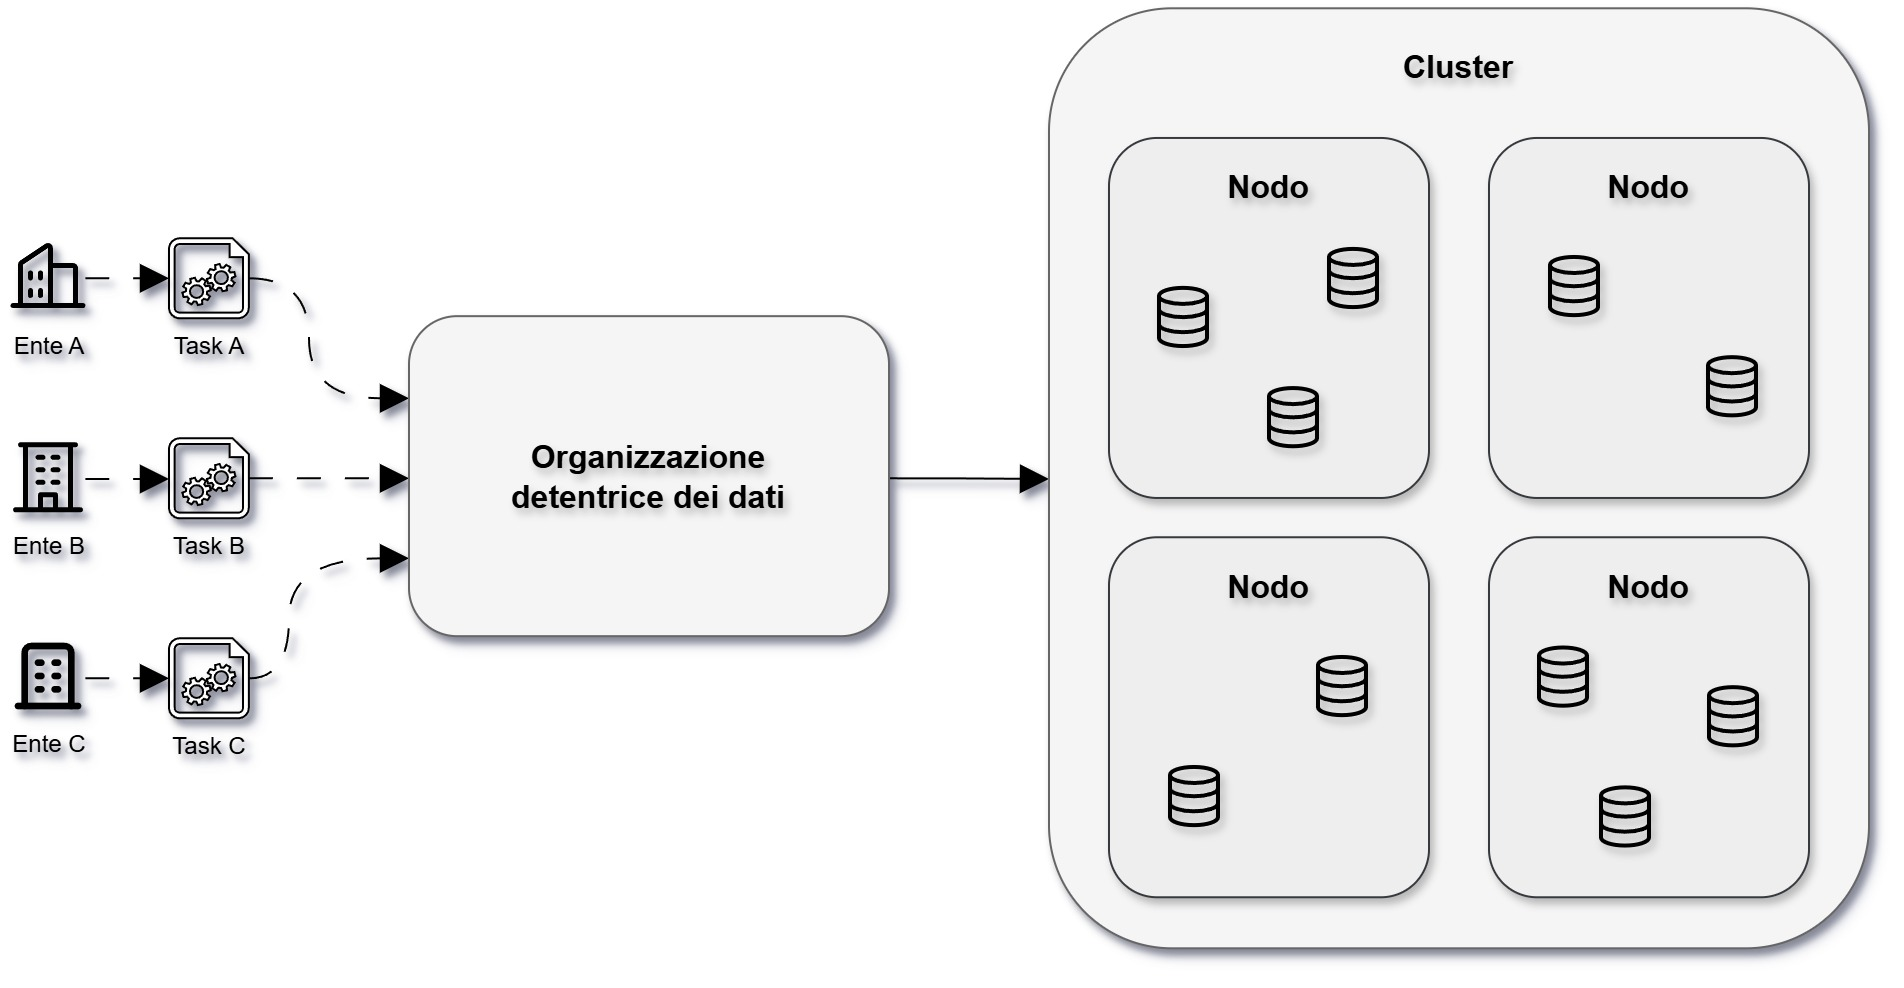
\includegraphics[width=\textwidth]{immagini/esempio.jpg}
    \caption{Enti esterni sottomettono task a un'organizzazione che detiene i dati, distribuiti sui nodi di un cluster.}
    \label{fig:esempio_contesto}
\end{figure}

A prima vista il compito dell'organizzazione potrebbe sembrare semplice, ovvero ricevere un task e mandarlo in esecuzione su un nodo che disponga dei dati richiesti e delle risorse necessarie, ma in realtà ogni richiesta porta con sé un insieme di vincoli che vanno ben oltre la semplice disponibilità di dati e risorse, e che nascono piuttosto dalla natura dei dati coinvolti. Alcuni dataset potrebbero contenere informazioni personali o comunque sensibili, sottoposte a normative come il GDPR che regolano in quali territori possano essere conservate ed elaborate, e un task che li utilizza non potrebbe quindi essere eseguito ovunque; altri, invece, potrebbero richiedere che il nodo su cui vengono trattati offra garanzie di sicurezza adeguate. Quando poi i dati necessari non si trovano già sul nodo scelto, occorre chiedersi se sia lecito farli trasferire e quanto costi farlo, tenendo presente che per alcuni di essi lo spostamento potrebbe essere del tutto escluso.

C'è infine un aspetto meno evidente, legato a ciò che accade una volta terminata l'esecuzione di un task. Un'elaborazione non scompare del tutto alla sua conclusione, ma può lasciare sul nodo che l'ha ospitata delle tracce residue dei dati utilizzati, le quali assumono particolare importanza quando i soggetti che si alternano su quel nodo sono in concorrenza tra loro. Se, ad esempio, l'ente A e l'ente B operano nello stesso settore e un task di A viene eseguito su un nodo che ha appena trattato dati riservati di B, si apre un potenziale canale di esposizione tra i due, anche in assenza di qualunque errore o comportamento scorretto da parte dell'organizzazione. Ne segue che la scelta del nodo non può basarsi soltanto su come quel nodo è fatto, ma deve tenere conto anche di ciò che vi è stato eseguito in precedenza.

Lo scenario appena descritto non è legato a un caso particolare, e le stesse esigenze si potrebbero ritrovare in contesti molto diversi tra loro. Ad esempio, un consorzio di ospedali che raccoglie e conserva i dati clinici dei propri pazienti può metterli a disposizione di gruppi di ricerca esterni che sottomettono analisi, con il vincolo che i dati non lascino l'istituto o il paese di origine; oppure un istituto finanziario che raccoglie informazioni di mercato e dati sui propri clienti può renderle disponibili a più società di consulenza esterne, alcune delle quali in concorrenza tra loro, e deve allora garantire che le informazioni di clienti concorrenti restino separate; oppure ancora un'infrastruttura di ricerca scientifica su larga scala, che raccoglie dati da più osservatori o strumenti, può dover rispettare sia vincoli di riservatezza legati a chi li finanzia sia l'impossibilità pratica di spostare i volumi più ingenti, per cui i gruppi di ricerca esterni sottomettono le proprie computazioni, che vengono eseguite direttamente dove i dati già si trovano. 

In tutti questi casi cambiano i dati, gli attori e le normative di riferimento, ma il problema di fondo resta lo stesso, rimanendo indipendente dal dominio applicativo: decidere su quale nodo distribuire una computazione che richiede determinati dati, rispettando l'insieme di vincoli che li riguardano. Per questo motivo, la soluzione sviluppata in questa tesi non è pensata per un singolo caso d'uso, ma per poter essere adattata a ciascuno di questi contesti definendo di volta in volta le regole che lo governano.

Tuttavia, una decisione come quella appena descritta non può essere lasciata a chi sottomette la richiesta. Gli enti esterni non hanno visibilità sull'infrastruttura, non sanno dove si trovino i dataset né quali nodi siano adatti ad accogliere la loro computazione, e non sarebbe nemmeno opportuno che potessero influenzarne la scelta, dato che sono proprio loro i soggetti da cui i dati vanno protetti. Le regole devono quindi essere stabilite da chi detiene i dati e applicate in modo uniforme a ogni richiesta, senza fare affidamento sulla correttezza di chi la invia. Questa tesi affronta il problema proponendo un insieme di politiche definite a livello di sistema, che stabiliscono quali assegnazioni siano ammissibili e quali tra queste siano preferibili, dandone prima una descrizione formale rigorosa, per poi realizzarle concretamente all'interno di un'infrastruttura reale.

% ------------------------------------------------------------ %

\section{Lavori Correlati}
\label{sec:stato_arte}

Il problema affrontato in questa tesi tocca diversi filoni di ricerca, ciascuno dei quali ne coglie un aspetto distinto. Da un lato ci sono vincoli normativi, come quelli legati alla \emph{data sovereignty} e alla geo-localizzazione dei dati, che impongono di tenere conto della posizione dei nodi quando si decide dove eseguire una computazione; dall'altro la \emph{data locality} guarda al problema da un'angolazione opposta, suggerendo di avvicinare il calcolo ai dati per contenerne il costo di trasferimento. A questi si affiancano i modelli formali per la gestione \emph{security-aware} delle risorse in scenari distribuiti, e il fenomeno della \emph{data remanence}, che insieme al modello \emph{Chinese Wall} guida la protezione dalle tracce lasciate dall'elaborazione, isolando tra loro esecuzioni successive in conflitto di interesse. Chiudono il quadro i lavori sullo scheduling \emph{policy-driven} in Kubernetes, che costituiscono il riferimento implementativo più vicino.

Questi aspetti vengono generalmente trattati in modo separato, mentre il contributo di questa tesi si colloca proprio alla loro intersezione. Le sottosezioni seguenti li ripercorrono singolarmente, chiarendo per ciascuno cosa viene ripreso e cosa invece cambia nell'impostazione di questa tesi.

% ------------------------------------------------------------ %

\subsection{Data Sovereignty e Geo-Localizzazione dei Dati}
\label{subsec:sovranita_dati_correlati}

Tra i vincoli che gravano sui dati, quelli legati alla sovranità sono forse i più importanti: il concetto di sovranità del dato, nella maggior parte dei casi, ruota attorno all'idea di un controllo effettivo sul luogo e sulle modalità con cui le informazioni possono essere conservate ed elaborate~\cite{data-sovereignty-review}. Le normative traducono questa esigenza in obblighi sempre più stringenti di localizzazione, che spesso non si limitano a chiedere una copia locale ma vietano il trasferimento all'estero~\cite{oecd-data-localisation}, facendo diventare così la collocazione delle risorse un problema di conformità. Rispetto a ciò, diversi lavori hanno proposto strategie di collocazione dei dati sensibili alla posizione geografica e alle regolamentazioni vigenti~\cite{geolocation-aware-data-placement, location-aware-data-placement}. Però, il focus di queste proposte resta il \emph{dove risiedono} i dati; il problema affrontato in questa tesi riguarda invece il \emph{dove eseguire} le computazioni che utilizzano quei dati, portando gli stessi vincoli dentro il processo di scheduling.

% ------------------------------------------------------------ %

\subsection{Data Locality e Costo di Trasferimento}
\label{subsec:data_locality_correlati}

La \emph{data locality} ribalta invece la prospettiva iniziale: al posto di muovere i dati verso la computazione, si avvicina la computazione ai dati. Lo scheduling nei cluster data-intensive tende a privilegiare i nodi che già ospitano gli input richiesti, accettando anche di ritardare l'avvio di un task pur di eseguirlo vicino ai dati, per poter ridurre il traffico della rete~\cite{delay-scheduling, data-locality-investigation-mapreduce}. Lo stesso principio guida gli approcci di \emph{near-data processing}~\cite{beyond-the-wall-ndp}, che eseguono parte dell'elaborazione direttamente accanto alla memoria in cui i dati risiedono, e più in generale lo scheduling che assegna la computazione al nodo dove i suoi dati sono già presenti, così da non doverli spostare sulla rete~\cite{transfer-cost-aware-edge-scheduling}. In tutti questi casi eseguire vicino ai dati è una scelta che conviene ma non un obbligo, mentre in altri diventa l'unica strada percorribile: quando i volumi rendono impraticabile qualsiasi spostamento~\cite{bringing-computation-moea}, o quando certi dataset non possono in alcun modo lasciare il nodo in cui risiedono, e allora è la computazione a doversi spostare verso i dati, dato che questi ultimi non possono essere trasferiti~\cite{paradigm-non-transferable-dataset}. Rispetto a ciò, questa tesi eredita l'ottimizzazione del costo di trasferimento, mentre la non trasferibilità di alcuni dataset non entra come semplice costo da minimizzare, ma come una condizione che esclude a priori i nodi che non possono ospitarli. 

% ------------------------------------------------------------ %

\subsection{Modelli Formali per la Gestione Security-Aware delle Risorse}
\label{subsec:modelli_formali_correlati}

Più vicini allo spirito di questa tesi sono i modelli formali per la gestione \emph{security-aware} delle risorse in scenari cloud e multicloud. Il riferimento principale, da cui questo lavoro trae la propria impostazione, è un modello per l'allocazione di dati soggetti a requisiti di protezione~\cite{sec-aware-data-alloc-multicloud}, nel quale i servizi cloud disponibili vengono classificati rispetto a proprietà di sicurezza astratte, ciascuna con livelli ordinati definiti da condizioni sugli attributi concreti del servizio, mentre ogni risorsa da collocare dichiara la classe minima che il servizio deve garantire per poterla ospitare. Il modello proposto in questa tesi riprende questa struttura e la adatta a un altro contesto: a essere classificati per proprietà astratte sono i nodi del cluster, e a dichiarare requisiti su di essi sono sia i task da eseguire sia i dataset che questi consumano, così che l'ammissibilità di un nodo nell'ospitare un task diventa un confronto tra livelli nello stesso spazio in cui i nodi sono classificati. Nella stessa direzione si colloca anche il lavoro sul supporto ai requisiti di sicurezza nella gestione delle risorse cloud~\cite{supp-sec-req-res-management-cloud}, dove le esigenze di protezione espresse dalle parti coinvolte si traducono in vincoli sull'allocazione. 

Un'ulteriore fonte di ispirazione sono le metodologie per la selezione dei piani cloud~\cite{supporting-user-requirement-pref-cloud, cloud-plan-selection-req-multiple-app}, che valutano e classificano le alternative disponibili sulla base di molteplici requisiti e delle preferenze espresse dagli utenti; ne deriva l'idea che, tra le opzioni ammissibili, la scelta finale combini più criteri di valutazione. Da tutto questo, il modello proposto eredita due idee: descrivere i nodi per proprietà astratte su cui le entità esprimono i propri requisiti, e valutare le alternative ammissibili secondo criteri multipli. Cambia però l'oggetto della decisione, perché nei casi citati si stabilisce dove collocare i dati o quale piano scegliere, mentre qui si stabilisce a quale nodo affidare la computazione, portando gli stessi strumenti formali dentro il processo di scheduling, dove l'ammissibilità del nodo e il costo di accesso ai dati richiesti entrano nella decisione stessa e non a valle di essa.

% ------------------------------------------------------------ %

\subsection{Data Remanence e Isolamento tra Elaborazioni}
\label{subsec:chinese_wall_correlati}

Finora i vincoli considerati riguardano principalmente il luogo in cui i dati possono essere conservati o raggiunti dalla computazione. Però, come anticipato nella Sezione~\ref{sec:contesto}, anche ciò che accade dopo l'elaborazione è rilevante, dato che l'esecuzione di un task può lasciare sul nodo tracce dei dati utilizzati. Il fenomeno prende il nome di \emph{data remanence}, ed è documentato sia come problema generale in ambito cloud~\cite{survey-data-remanence-cloud}, sia a livello dei supporti fisici di memorizzazione~\cite{data-remanence-flash-memory}, dove frammenti dei dati o della loro elaborazione possono sopravvivere in memoria, nello storage effimero o nelle cache anche dopo la fine dell'esecuzione. In un nodo condiviso tra soggetti in concorrenza, questo residuo diventa il punto in cui potrebbe nascere un conflitto di interesse.

Il riferimento naturale per questo tipo di problema è il modello \emph{Chinese Wall} di Brewer e Nash~\cite{chinese-wall-brewer-nash}, nato in ambito finanziario per impedire che un soggetto acceda a informazioni di aziende in conflitto tra loro, erigendo un muro che gli vieta ogni accesso ulteriore ai concorrenti di chi ha già consultato. Dal modello originale sono poi nate diverse varianti che ne approfondiscono la memoria del soggetto e ne modificano la logica, rimettendo in discussione, ad esempio, la transitività della relazione di conflitto~\cite{chinese-wall-aggressive-lin}. Proprio tra queste osservazioni emerge un limite noto del modello classico: una volta costruito, un muro non viene mai rimosso, e l'assenza di un meccanismo che ne preveda il decadimento prima o poi porta inevitabilmente ogni soggetto a restare bloccato dai propri accessi passati~\cite{chinese-wall-kessler}. Questa tesi adotta questo principio di isolamento sull'asse nodo-task, applicandolo alla relazione tra un nodo condiviso e le esecuzioni di task che vi si susseguono, così come è già stato fatto ad esempio per l'isolamento fisico tra macchine virtuali in conflitto ospitate sullo stesso nodo di un'infrastruttura cloud~\cite{chinese-wall-cloud-nodes-data}, con un'inversione di prospettiva rispetto alla memoria di cui parla il modello classico, che per una persona fisica è la rappresentazione della sua conoscenza accumulata, mentre per un nodo di calcolo è un componente fisico concreto. Lo stato lasciato dalle elaborazioni passate entra così a pieno titolo nelle politiche di isolamento tra nodi e task, offrendo allo stesso tempo una via d'uscita dalla \emph{starvation} che nel modello originale restava un problema aperto; questo perché, a differenza della memoria di una persona, quella di un nodo può essere ripulita, rimuovendo materialmente le tracce delle elaborazioni precedenti e facendo così decadere il muro che esse avevano imposto.

% ------------------------------------------------------------ %

\subsection{Scheduling Policy-Driven in Kubernetes}
\label{subsec:k8s_correlati}

Passando alla parte implementativa, il riferimento più diretto è dato da due lavori sullo scheduling \emph{policy-driven} in Kubernetes~\cite{policy-driven-sec-aware-scheduling-k8s, secure-k8s-workload-deployment}. Il problema da cui partono è che i vincoli di selezione del nodo vanno scritti a mano nella specifica di ogni singolo \texttt{Pod}, con il rischio di configurazioni fragili e soggette a errori; la loro proposta consiste nel definire le politiche una volta sola a livello di cluster e affidarne l'applicazione automatica a OPA Gatekeeper, che in fase di ammissione traduce etichette di alto livello nei vincoli di scheduling corrispondenti e rifiuta le richieste che violano le politiche stabilite, con un impatto trascurabile sulle prestazioni. Con questi lavori la tesi condivide l'impostazione di fondo, ovvero governare lo scheduling tramite politiche definite centralmente e realizzarlo sui meccanismi di estensione di Kubernetes, riprendendone l'uso di OPA Gatekeeper per la validazione delle richieste. Però, il loro intervento si limita alla fase di ammissione, dopo la quale la scelta del nodo resta allo scheduler nativo, che si basa su vincoli fissati una volta per tutte al momento della creazione del \texttt{Pod}~\cite{k8s-scheduler}. Per il problema affrontato qui questo non basta, perché assieme alle politiche statiche di questo tipo servono anche politiche dinamiche, come quella di isolamento ispirata alla Chinese Wall precedentemente discussa, che dipendono dallo stato che un nodo ha accumulato nel tempo, oltre ad altri criteri come il costo di accesso ai dati richiesti: condizioni dinamiche di questo genere non possono essere fissate in ammissione e vanno valutate nel momento stesso in cui un nodo viene scelto. Ne consegue la necessità di estendere anche lo scheduler nativo di Kubernetes, portando la logica delle politiche fino alla fase di scheduling vera e propria~\cite{k8s-scheduler-framework}.

% ------------------------------------------------------------ %

\section{Obiettivi e Contributi}
\label{sec:obiettivi}

Il problema delineato nella Sezione~\ref{sec:contesto} potrebbe apparire come una semplice variante dello scheduling tradizionale, ma diversi elementi lo rendono tutt'altro che banale. Il primo è che i vincoli provengono da fonti diverse e vanno soddisfatti simultaneamente, senza che esista un ordine naturale in cui valutarli; le caratteristiche richieste dal task, i requisiti di protezione di ciascun dataset, i limiti geografici imposti dalle normative e l'ammissibilità di un eventuale trasferimento si combinano tra loro, e talvolta spingono in direzioni opposte, come accade quando la convenienza di eseguire un task vicino ai propri dati si scontra con un nodo che, pur ospitandoli, non offre le garanzie richieste. Il secondo è che una parte di questi vincoli non dipende soltanto da come un nodo è fatto, ma da ciò che è accaduto in passato, vincolando quindi la decisione a uno stato che evolve a ogni assegnazione e che va periodicamente ripristinato, per evitare che i nodi finiscano per diventare inutilizzabili. Il terzo riguarda la separazione delle responsabilità precedentemente discussa, secondo cui chi sottomette un task è proprio il soggetto da cui i dati vanno protetti, e per questo non ci si può affidare allo stesso per indicare i vincoli da rispettare, ma è il sistema a doverli applicare uniformemente a ogni richiesta. L'ultimo, non per importanza, è che tutto questo deve poter essere realizzato all'interno di un orchestratore reale, i cui meccanismi nativi non prevedono né vincoli legati alla protezione dei dati né decisioni che dipendano dallo stato accumulato dai nodi.

L'obiettivo del lavoro è quindi progettare e realizzare un sistema di scheduling \emph{policy-driven} per task che consumano dataset soggetti a vincoli di protezione, con due contributi principali. Da una parte un modello formale che descrive matematicamente le entità coinvolte, le politiche che ne governano i vincoli e il criterio con cui individuare il nodo migliore tra quelli ammissibili, riprendendo dalla letteratura le idee usate per la distribuzione dei dati e la selezione delle risorse e adattandole alla distribuzione della computazione, con l'aggiunta di una politica di isolamento ispirata al modello \emph{Chinese Wall}, che tiene conto della storia delle elaborazioni su ciascun nodo. Dall'altra l'implementazione del modello in ambiente Kubernetes, sfruttando i meccanismi di estensione nativi per portare la valutazione delle politiche dalla fase di ammissione delle richieste fino alla scelta effettiva del nodo.

% ------------------------------------------------------------ %

\section{Organizzazione della Tesi}
\label{sec:organizzazione}

Il resto dei capitoli di questa tesi va dalla definizione del problema alla sua realizzazione concreta. Il Capitolo~\ref{cap:definizione} inquadra lo scenario applicativo e gli attori coinvolti, fissa le assunzioni entro cui il sistema opera e introduce la formalizzazione dei concetti di base, per poi enunciare le proprietà che il sistema garantisce per costruzione. Il Capitolo~\ref{cap:modello} costituisce il nucleo teorico della tesi, dove si sviluppa il modello di scheduling policy-driven, dalla classificazione dei nodi per proprietà astratte alla compatibilità tra requisiti delle entità e caratteristiche dei nodi, passando per i vincoli geografici, la staticità dei dataset e il costo del loro trasferimento, fino al trattamento dei conflitti di interesse tra contesti e all'isolamento dei nodi rispetto ai task, chiudendo con un esempio applicativo completo che mostra il modello all'opera. Il Capitolo~\ref{cap:implementazione} descrive come questo modello venga tradotto in un sistema funzionante in ambiente Kubernetes, sfruttando i meccanismi di estensione nativi della piattaforma per realizzare la validazione delle richieste, la loro traduzione in unità schedulabili e lo scheduler personalizzato che ne implementa filtraggio e ottimizzazione. Il Capitolo~\ref{cap:valutazione} raccoglie la valutazione sperimentale del sistema, concentrandosi sulla componente dinamica il cui comportamento dipende dallo stato del cluster, e ne analizza l'impatto sulla latenza di scheduling al variare del grado di conflitto e della frequenza di sanificazione dei nodi. Infine, il Capitolo~\ref{cap:conclusioni} trae le conclusioni del lavoro svolto alla luce di quanto emerso lungo l'intero elaborato, discutendone le possibili direzioni di sviluppo future.
\chapter{Definizione del Problema}
\label{cap:definizione}

In questo capitolo viene presentata la definizione del problema affrontato nella tesi, con l'obiettivo di chiarire il contesto, gli attori coinvolti e i vincoli che caratterizzano il sistema. Dopo una prima descrizione generale dello scenario applicativo, verranno introdotte le principali assunzioni adottate, seguite dalla formalizzazione dei concetti base, dalla formulazione del problema e dalle proprietà che il sistema garantisce.

% ------------------------------------------------------------ %

\section{Scenario e Architettura di Riferimento}
\label{sec:scenario_applicativo}

Il sistema oggetto di questa tesi affronta il problema della distribuzione e schedulazione di task computazionali in un insieme di nodi di un cluster distribuito, nel rispetto di un insieme di politiche volte a governare le proprietà dei nodi di esecuzione, la gestione dei dati necessari all'elaborazione e i vincoli associati ai task stessi.

Un insieme di utenti esterni sottomette richieste di esecuzione di task al sistema, in cui ogni task sarà caratterizzato dalle proprie proprietà e dai propri requisiti, primi fra tutti i dataset su cui la computazione si basa, oltre a ulteriori vincoli relativi, ad esempio, alle caratteristiche del nodo di esecuzione o a vincoli di sovranità geografica dei dati. Inoltre, la semantica interna dei task sarà considerata irrilevante ai fini della distribuzione e schedulazione sul cluster: ciò che conta sono esclusivamente le caratteristiche e i vincoli associati che li compongono.

Ogni nodo del cluster è caratterizzato da un insieme di proprietà, tra le quali ad esempio la localizzazione geografica o il livello di sicurezza offerto, e ospita localmente un sottoinsieme dei dataset disponibili nel sistema. Inoltre, i suddetti dataset non sono risorse omogenee, ma ciascuno è associato a un proprio insieme di requisiti di protezione che ne vincolano la collocazione e l'eventuale trasferimento verso altri nodi del cluster. Facendo un esempio di un ipotetico scenario reale, un dataset soggetto a normative di sovranità geografica dei dati non può essere trasferito o acceduto in remoto da nodi situati al di fuori di una determinata area di competenza, oppure un dataset con requisiti di confidenzialità elevati non può risiedere su nodi il cui livello di sicurezza risulti insufficiente.

Di conseguenza, quando un task viene sottomesso al sistema, è necessario determinare su quale nodo del cluster debba essere eseguito. Questa decisione deve rispettare un insieme di politiche che operano principalmente su tre livelli distinti:
\begin{itemize}
    \item Al primo livello, è necessario verificare che il task stesso sia ammissibile nel sistema, indipendentemente da qualunque nodo candidato: alcune politiche possono infatti determinarne l'ammissibilità esclusivamente sulla base delle sue proprietà o dei suoi requisiti, senza alcun riferimento alla compatibilità con un nodo specifico;
    \item Al secondo livello, le politiche valutano la compatibilità tra le proprietà e i requisiti del task sottomesso da un utente e le caratteristiche dei nodi candidati;
    \item Al terzo livello, è necessario verificare che l'eventuale trasferimento o accesso remoto dei dataset richiesti dal task verso il nodo candidato sia ammissibile rispetto alle politiche di protezione ad essi associate.
\end{itemize}

Qualora il task non risulti ammissibile rispetto al primo livello, oppure nessun nodo dovesse soddisfare gli altri due livelli di vincolo, il task dell'utente non sarà schedulato nel sistema. Altrimenti, tra i nodi validi che rispettano tutti i vincoli delle politiche, il sistema seleziona quello ottimale secondo un criterio che terrà in considerazione più fattori, tra i quali, ad esempio, il costo associato al trasferimento o all'accesso dei dataset remoti oppure le risorse attualmente disponibili sui nodi candidati.

Il processo di distribuzione dei task è quindi, come illustrato nella Figura~\ref{fig:scenario}, strutturato in due fasi logiche. Una prima fase di \emph{policy evaluation}, in cui il task viene prima validato rispetto alle politiche di ammissibilità e, se ammesso, vengono filtrati i nodi non compatibili con i vincoli e i requisiti del task e dei dataset richiesti; e una seconda fase di \emph{optimal scheduling}, nella quale, tra i nodi ammissibili, viene selezionato quello ottimale.

\begin{figure}[htb]
    \centering
    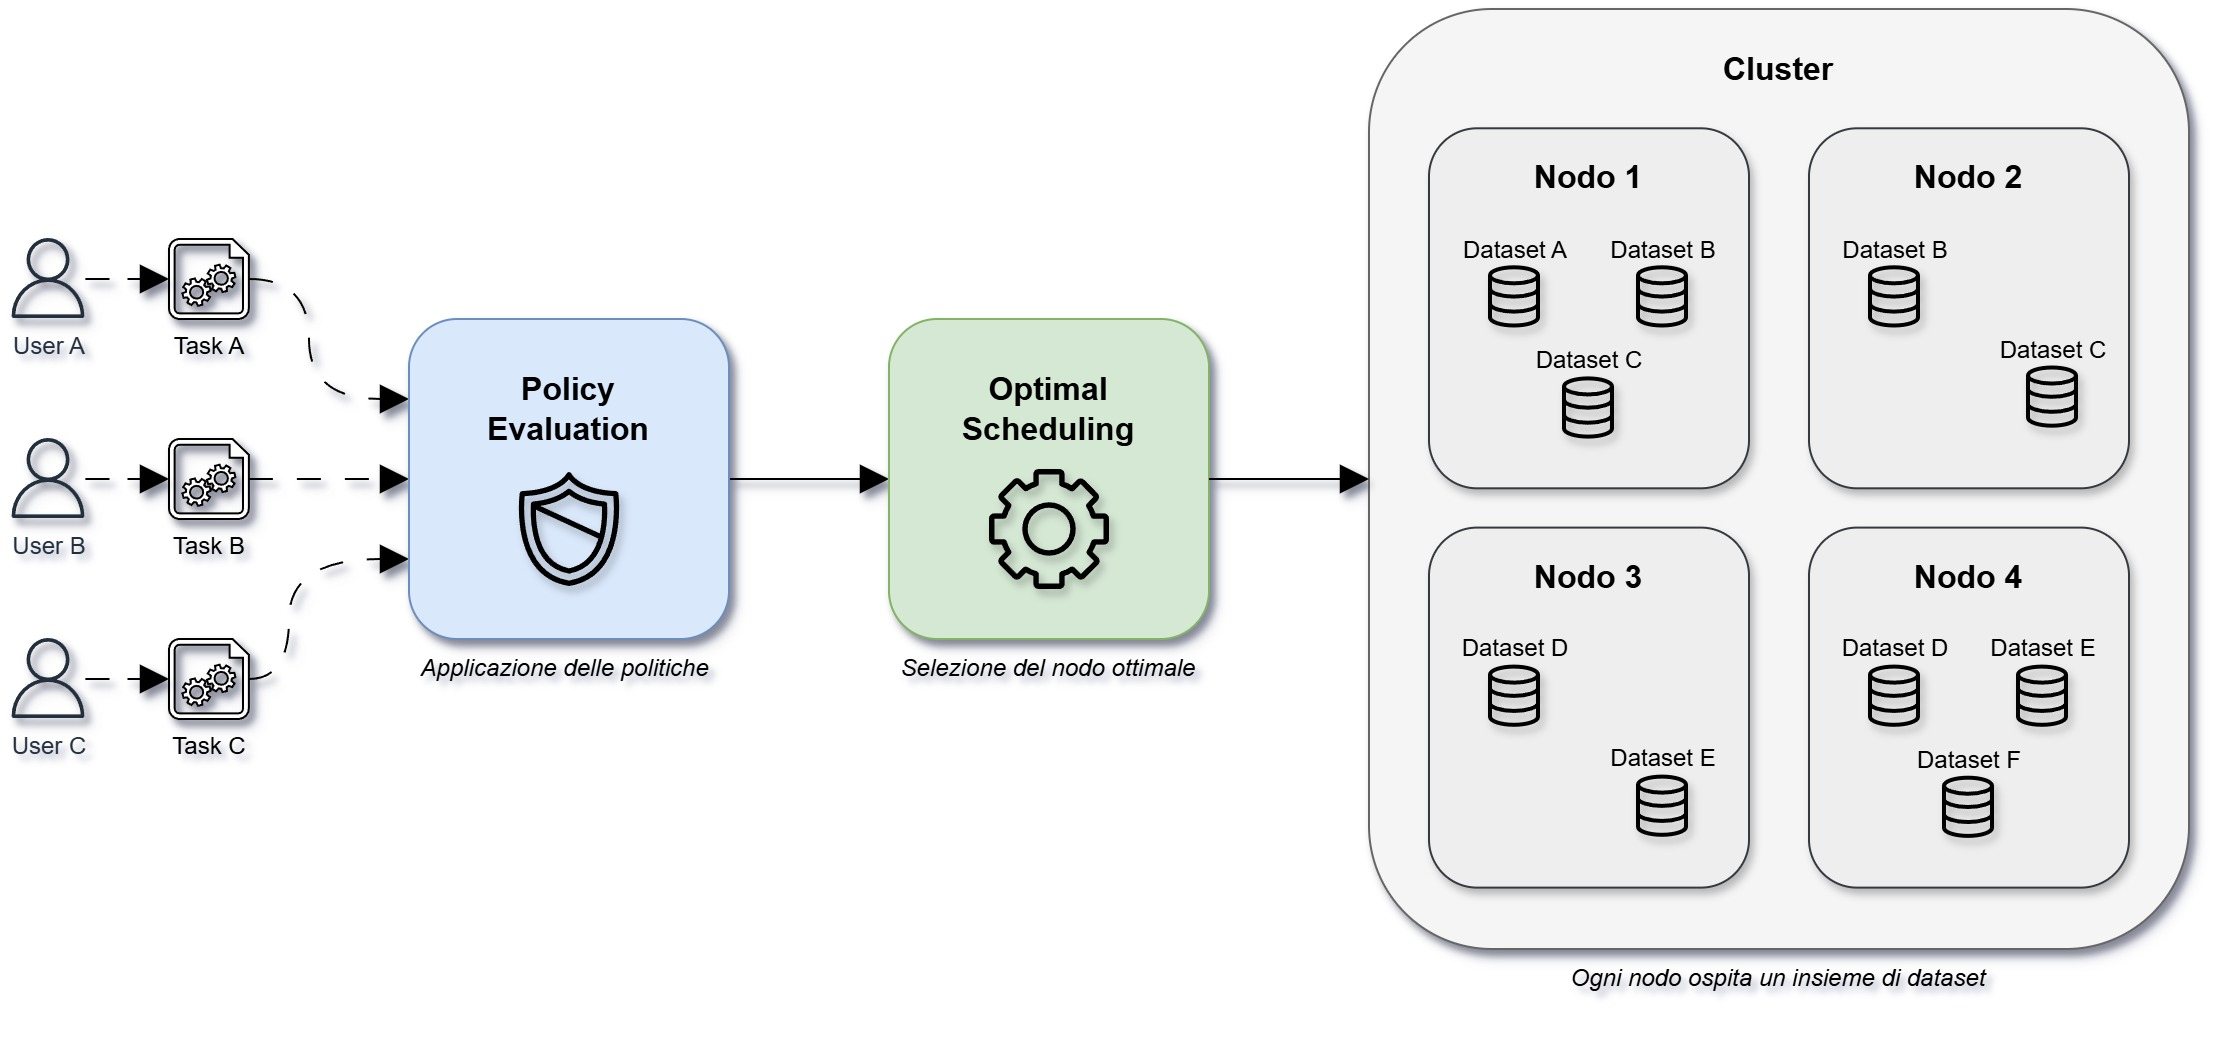
\includegraphics[width=\textwidth]{immagini/scenario.jpg}
    \caption{Architettura di riferimento del sistema.}
    \label{fig:scenario}
\end{figure}

L'aspetto più importante del problema riguarda la separazione delle responsabilità tra gli attori del sistema. Gli utenti esterni al sistema richiederanno l'esecuzione di task senza avere visibilità né controllo diretto sulla struttura interna del cluster o sulla distribuzione dei dataset: la loro interazione con il sistema si limita alla specifica dei requisiti del task. Invece, le politiche che governano la distribuzione sono definite a livello di sistema e hanno come obiettivo la protezione delle risorse rispetto agli utenti che le richiedono, garantendo che l'esecuzione avvenga soltanto in condizioni di compatibilità con il modello delle politiche.

Il problema affrontato in questa tesi consiste quindi nel progettare e realizzare un sistema \emph{policy-driven}, implementato in ambiente Kubernetes, in grado di ricevere richieste di esecuzione di task da parte di utenti esterni, valutarne i requisiti rispetto alle politiche associate alle risorse del cluster (definite secondo il modello che verrà introdotto nei capitoli successivi) e determinare, quando possibile, il nodo di esecuzione ottimale tra quelli che soddisfano tali vincoli. 

I lavori correlati che affrontano il problema dello scheduling \emph{policy-driven} in Kubernetes presentati in~\cite{policy-driven-sec-aware-scheduling-k8s, secure-k8s-workload-deployment} costituiscono un riferimento per il presente lavoro. Tuttavia, questa tesi si differenzia da tale approccio per l'introduzione esplicita di un modello formale dei vincoli tra le entità del sistema, seguendo un approccio simile a quanto già proposto in letteratura per la gestione e la classificazione delle risorse cloud in~\cite{sec-aware-data-alloc-multicloud, supp-sec-req-res-management-cloud, model-decision-data-storage-cloud}.

% ------------------------------------------------------------ %

\section{Assunzioni Preliminari}
\label{sec:assunzioni_preliminari}

Per descrivere il problema in modo più chiaro, è utile introdurre alcune assunzioni preliminari che ne delimitano il contesto e rendono il modello più gestibile. Queste assunzioni nascono dall'esigenza di mantenere il problema ben definito e affrontabile nell'ambito della tesi.

\paragraph{Distribuzione dei dataset}
\label{ass:dataset_distribuzione}

Ogni dataset è memorizzato localmente su uno o più nodi del cluster e, all'inizializzazione del sistema, si assume che la distribuzione iniziale dei dataset sia corretta, ovvero che non violi alcun vincolo associato ai dataset stessi. L'obiettivo del sistema non è quindi gestire la collocazione persistente dei dataset all'interno del cluster, ma valutare l'eventuale trasferimento logico o l'accesso remoto di un dataset verso il nodo selezionato per l'esecuzione di un task, nei casi in cui non sia già disponibile localmente su quel nodo. A tale operazione è associato un costo proporzionale alla dimensione del dataset, nota a priori, e la sua ammissibilità è subordinata al rispetto delle politiche di protezione associate al dataset. Questa scelta separa dunque il problema della collocazione persistente dei dataset, incluso lo spostamento fisico e la gestione della consistenza nel cluster, dal problema principale affrontato dal sistema, ovvero l'assegnazione dei task ai nodi e la valutazione del costo e dei vincoli dell'accesso remoto ai dati. In questo modo, il sistema integra costo e vincoli del trasferimento direttamente nel processo di selezione del nodo ottimale basandosi unicamente sui metadati necessari alla valutazione, senza dover realizzare un sottosistema dedicato allo spostamento fisico dei dati. Considerare anche il problema della distribuzione persistente dei dati introdurrebbe infatti una complessità aggiuntiva indipendente dagli obiettivi principali del lavoro. Il problema dell'allocazione fisica dei dati in un cluster o in ambiente cloud è comunque un aspetto ampiamente approfondito, ad esempio, nei lavori presentati in~\cite{sec-aware-data-alloc-multicloud, model-decision-data-storage-cloud}.

\paragraph{Visione globale del cluster}
\label{ass:visione_globale}

Al momento della sottomissione di un task da parte di un utente, il sistema dispone di una visione globale dello stato del cluster, che comprenderà sia le caratteristiche dei nodi sia la distribuzione corrente dei dataset su di essi. Questa assunzione è necessaria affinché il processo decisionale possa operare su informazioni complete e coerenti. Nel contesto di questa tesi tale aspetto è considerato risolto a livello infrastrutturale, in quanto Kubernetes espone nativamente un'interfaccia centralizzata per l'osservazione dello stato del cluster~\cite{k8s-comunication-nodes-control-plane, k8s-api}.

\paragraph{Esecuzione atomica dei task}
\label{ass:task_atomicita}

Ogni task viene eseguito interamente su un singolo nodo del cluster e non è prevista né la suddivisione di esso tra più nodi né la sua migrazione verso un nodo diverso dopo la sua assegnazione: la decisione di scheduling è quindi considerata definitiva al momento dell'assegnazione del task su un nodo. Questa ipotesi è coerente con il modello adottato da Kubernetes, che garantisce nativamente che ogni \texttt{Pod}, ossia la più piccola unità di lavoro che in questo contesto rappresenta il task, venga assegnato ed eseguito su un unico nodo, come descritto in~\cite{k8s-pods-atomic-node}.

\paragraph{Indipendenza dalla semantica dei task}
\label{ass:task_black_box}

Il sistema è indipendente dalla semantica interna dei task, che sono trattati come \emph{black-box} e considerati esclusivamente in termini delle loro proprietà, dei requisiti dichiarati e degli eventuali vincoli aggiuntivi rilevanti per il processo di assegnazione. Questa astrazione è necessaria per garantire la generalità del modello: un sistema dipendente dalla logica interna dei task risulterebbe infatti applicabile solo a domini di lavoro specifici, mentre l'obiettivo della tesi è definire un approccio di schedulazione generale indipendente dal tipo di operazioni che verranno eseguite.

\paragraph{Presenza di almeno un dataset richiesto}
\label{ass:dataset_minimo}

Ogni task richiede per la propria esecuzione almeno un dataset, coerentemente con il fatto che la computazione si fonda su di esso. Questa assunzione delimita il campo di applicazione del modello all'obiettivo della tesi, ovvero la distribuzione di task che utilizzano dataset soggetti a vincoli di protezione: un task privo di dataset richiesti non attiverebbe nessuna politica di protezione dei dati, ricadendo in un problema basilare di puro scheduling task-nodo.

% ------------------------------------------------------------ %

\section{Formalizzazione dei Concetti Base}
\label{sec:formalizzazione_base}

In questa sezione si introduce la formalizzazione del problema della tesi descritto nella Sezione~\ref{sec:scenario_applicativo}. L'obiettivo è rendere precisi i concetti di nodo, dataset, task e politica, e formulare il problema di assegnazione dei task in termini matematici. Le strutture introdotte in seguito saranno volutamente astratte e non approfondite: la loro descrizione concreta, ossia la definizione delle proprietà specifiche, dei vincoli delle entità e del contenuto delle politiche, è rimandata al Capitolo~\ref{cap:modello}.

% ------------------------------------------------------------ %

\subsection{Entità del Sistema e Distribuzione dei Dataset}
\label{subsec:entita_sistema}

Il sistema è definito da quattro insiemi fondamentali: l'insieme dei nodi $\mathcal{N}$, inteso come l'insieme dei nodi del cluster attivi e raggiungibili al momento della valutazione, l'insieme dei dataset disponibili nel sistema $\mathcal{D}$, l'insieme dei task $\mathcal{T}$ e l'insieme degli emittenti $\mathcal{I}$ (detti \emph{issuer}), che corrispondono ai soggetti che sottomettono i task nel sistema. A ogni task $t \in \mathcal{T}$ è associato il proprio emittente mediante la funzione:
\begin{equation}
    iss: \mathcal{T} \rightarrow \mathcal{I}
\end{equation}
tale che $iss(t)$ identifica l'issuer del task $t$. Inoltre, a ciascun task è associato l'insieme dei dataset necessari alla sua esecuzione, definito da:
\begin{equation}
    req: \mathcal{T} \rightarrow 2^\mathcal{D}
\end{equation}
ottenendo quindi $req(t) \subseteq \mathcal{D}$. Ad esempio, un task che per la sua esecuzione richiede due dataset $d_1$ e $d_2$ avrà $req(t) = \left\{ d_1,\, d_2 \right\}$.

Il primo elemento da formalizzare è la distribuzione dei dataset sui nodi del cluster. Poiché ogni dataset può essere disponibile su più nodi contemporaneamente, la collocazione dei dataset è definita dalla funzione descritta nella seguente Definizione~\ref{def:allocazione_dataset}. Un approccio simile è adottato in~\cite{sec-aware-data-alloc-multicloud}, dove la distribuzione di dati in scenari multicloud è modellata tenendo conto di requisiti di protezione associati a ciascuna risorsa.

\begin{definition}[Allocazione dei dataset]
    \label{def:allocazione_dataset}
    Lo stato di allocazione dei dataset nei nodi del cluster è definito dalla funzione:
    \begin{equation}
        \lambda: \mathcal{D} \rightarrow 2^\mathcal{N}
    \end{equation}
    dove $\lambda(d)$ indica l'insieme dei nodi in cui il dataset $d \in \mathcal{D}$ è disponibile localmente al momento della chiamata di funzione.
\end{definition}

Ad esempio, se attualmente i dataset $d_1$ e $d_2$ sono presenti localmente sui nodi $n_1$ e $n_2$, si avrà $\lambda(d_1) = \lambda(d_2) = \{n_1,\, n_2\}$. 
% La questione della dipendenza di $\lambda$ dal tempo, rilevante nei casi in cui l'allocazione evolve a seguito di trasferimenti tra nodi, sarà discussa nel Capitolo~\ref{cap:modello}, dove verrà chiarito in quale momento del processo di schedulazione lo stato di allocazione viene osservato dal sistema.

% ------------------------------------------------------------ %

\subsection{Famiglie di Politiche e Soddisfacibilità}
\label{subsec:famiglie_politiche}

Il cuore del sistema è costituito dall'insieme delle politiche, indicato con $\mathcal{C}$, che governano l'assegnazione dei task e l'eventuale trasferimento dei dati richiesti. Una politica esprime un vincolo che dovrà essere soddisfatto affinché un nodo possa essere considerato un candidato valido per l'esecuzione di un task. 

Le politiche in $\mathcal{C}$ operano a tre livelli distinti e coprono tre aspetti complementari del processo di assegnazione. Il primo sottoinsieme, denotato da $\mathcal{C_A} \subseteq \mathcal{C}$, raccoglie le politiche che determinano l'ammissibilità di un task $t$ nel sistema indipendentemente da qualunque nodo candidato: a differenza dei successivi sottoinsiemi, una politica in $\mathcal{C_A}$ non valuta la compatibilità tra il task e un nodo, ma stabilisce se il task possa essere preso in carico dal sistema solamente sulla base delle proprie proprietà, del proprio emittente, o dello stato corrente del sistema. Il secondo sottoinsieme, denotato da $\mathcal{C_T} \subseteq \mathcal{C}$, raccoglie le politiche che valutano la compatibilità diretta tra i requisiti del task $t$ e le caratteristiche del nodo candidato $n$: ad esempio, verificando che il nodo offra un certo livello di sicurezza o disponga delle risorse computazionali richieste. Il terzo sottoinsieme, denotato da $\mathcal{C_D} \subseteq \mathcal{C}$, regola invece il possibile trasferimento o accesso remoto dei dataset in $req(t)$ sul nodo candidato $n$: ad esempio, imponendo che il trasferimento di un dataset avvenga soltanto verso nodi situati in una determinata area geografica di riferimento, oppure che certi dataset non vengano trasferiti affatto.

I tre sottoinsiemi non sono necessariamente disgiunti tra loro: una politica che impone requisiti di sicurezza su un nodo può regolare contemporaneamente il trasferimento di dati verso di esso, appartenendo quindi sia a $\mathcal{C_T}$ sia a $\mathcal{C_D}$. Tuttavia, la loro unione copre l'intero insieme delle politiche:
\begin{equation}
    \mathcal{C} = \mathcal{C_A} \cup \mathcal{C_T} \cup \mathcal{C_D}
\end{equation}

Poiché le politiche operano su entità distinte, ovvero coppie nodo-task, coppie nodo-dataset e il task considerato indipendentemente da un nodo, si introduce una notazione di soddisfacibilità che copre tutti i casi. Per una politica $c \in \mathcal{C_T} \cup \mathcal{C_D}$, il vincolo riguarda la compatibilità tra un nodo candidato e il task o un dataset richiesto: scriviamo $n \models_t c$ per indicare che il nodo $n \in \mathcal{N}$ soddisfa la politica $c$ rispetto al task $t \in \mathcal{T}$, e $n \models_d c$ per indicare che il nodo $n$ soddisfa la politica $c$ rispetto al dataset $d \in \mathcal{D}$, ovvero che il possibile trasferimento di $d$ su $n$ è ammissibile secondo $c$. Invece, per una politica $c \in \mathcal{C_A}$ il vincolo riguarda esclusivamente il task, indipendentemente da qualunque nodo candidato: scriviamo $t \models c$ per indicare che il task $t \in \mathcal{T}$ soddisfa la politica $c$ rispetto al sistema, ovvero che $t$ è ammissibile nel sistema secondo $c$.

La stessa notazione si estende in modo naturale a un'intera famiglia di politiche, intendendo che ciascuna delle politiche che la compongono sia soddisfatta:
\begin{align}
    t \models \mathcal{C_A} &\iff \forall\, c \in \mathcal{C_A} :\; t \models c \\
    n \models_t \mathcal{C_T} &\iff \forall\, c \in \mathcal{C_T} :\; n \models_t c \\
    n \models_d \mathcal{C_D} &\iff \forall\, c \in \mathcal{C_D} :\; n \models_d c
\end{align}
Si tratta di semplici abbreviazioni, che verranno usate nel seguito quando non serve distinguere le singole politiche di una famiglia.

\begin{definition}[Soddisfacibilità delle politiche]
    \label{def:politiche}
    Sia $\mathcal{C}$ un insieme di politiche che il sistema deve rispettare durante la fase di assegnazione di un task. Ogni politica $c \in \mathcal{C}$ è un predicato che definisce un vincolo sul processo di assegnazione. La soddisfacibilità globale di tutte le politiche $\mathcal{C}$ rispetto a un task $t \in \mathcal{T}$ per un nodo candidato $n \in \mathcal{N}$ è definita come:
    \begin{equation}
        n \models_t \mathcal{C}
        \iff
        \left( \bigwedge_{c \in \mathcal{C_A}} t \models c \right)
        \land
        \left( \bigwedge_{c \in \mathcal{C_T}} n \models_t c \right)
        \land
        \left( \bigwedge_{\substack{c \in \mathcal{C_D}\\ d \in req(t)}} n \models_d c \right)
    \end{equation}
    Tale condizione equivale a richiedere $t \models \mathcal{C_A}$, $n \models_t \mathcal{C_T}$ e $n \models_d \mathcal{C_D}$ per ogni $d \in req(t)$.
\end{definition}

La condizione $n \models_t \mathcal{C}$ stabilisce quindi che il nodo $n$ può ammettere l'esecuzione del task $t$ se e solo se sono soddisfatte contemporaneamente tutte le condizioni definite dalle diverse famiglie di politiche discusse. In particolare, il task deve essere prima di tutto ammissibile nel sistema rispetto alle politiche indipendenti dal nodo $\mathcal{C_A}$, il nodo deve soddisfare i vincoli di compatibilità task-nodo definiti in $\mathcal{C_T}$, e, per ogni dataset $d \in req(t)$ richiesto, deve risultare ammissibile il suo possibile trasferimento o accesso remoto su $n$ secondo tutte le politiche nodo-dataset appartenenti a $\mathcal{C_D}$.

Da questa struttura, combinandola con l'assunzione di distribuzione iniziale corretta dei dataset, segue un risultato immediato riguardo i dataset già disponibili localmente su un nodo candidato.

\begin{theorem}[Correttezza dei dataset locali rispetto a $\mathcal{C_D}$]
    \label{teo:correttezza_locale}
    Per ogni dataset $d \in \mathcal{D}$ e per ogni nodo $n \in \mathcal{N}$, se $d$ è disponibile localmente su $n$, allora $n$ soddisfa tutte le politiche in $\mathcal{C_D}$ rispetto a $d$:
    \begin{equation}
        n \in \lambda(d) \implies n \models_d \mathcal{C_D}
        \qquad
        \forall\, d \in \mathcal{D},\, \forall\, n \in \mathcal{N}
    \end{equation}
    \begin{proof}
        Si dimostra per induzione sul numero $k$ di trasferimenti di dataset avvenuti nel sistema. 
        
        \paragraph{Caso base ($k = 0$)} All'inizializzazione del sistema, per assunzione, la distribuzione iniziale dei dataset è corretta: per ogni $d \in \mathcal{D}$ e ogni $n \in \lambda(d)$, vale $n \models_d \mathcal{C_D}$.
        
        \paragraph{Passo induttivo ($k > 0$)} Si supponga che la proprietà valga dopo $k$ trasferimenti, ovvero che per ogni $d \in \mathcal{D}$ e ogni $n \in \lambda(d)$ valga $n \models_d \mathcal{C_D}$. Sia ora $n' \notin \lambda(d')$ un nodo verso cui viene richiesto il $(k+1)$-esimo trasferimento di un dataset $d' \in \mathcal{D}$. Il trasferimento è ammesso dal sistema se e solo se $n' \models_{d'} \mathcal{C_D}$. Si distinguono ora due casi:
        \begin{itemize}
            \item  Se la condizione non è soddisfatta, il trasferimento viene rifiutato e $\lambda(d')$ rimane invariato. La proprietà continua a valere per ipotesi induttiva;
            \item Se la condizione è soddisfatta, il trasferimento viene eseguito e $\lambda(d')$ viene aggiornato con:
            \begin{equation}
                \lambda(d') \leftarrow \lambda(d') \cup \{n'\}
            \end{equation}
            Per i nodi già appartenenti a $\lambda(d')$ la proprietà continua a valere per ipotesi induttiva, mentre per $n'$ siamo nel caso in cui $n' \models_{d'} \mathcal{C_D}$ è soddisfatta. Di conseguenza, la validità della proprietà si estende al nuovo insieme $\lambda(d')$.
        \end{itemize}
        Dato che la proprietà è preservata in entrambi i casi, è dimostrato per induzione che:
        \begin{equation}
            n \in \lambda(d) \implies n \models_d \mathcal{C_D}
            \qquad 
            \forall d \in \mathcal{D}, \; \forall n \in \mathcal{N}
        \end{equation}
        è valida in ogni stato raggiungibile del sistema.
    \end{proof}
\end{theorem}

% ------------------------------------------------------------ %

\subsection{Nodi Ammissibili e Funzione di Ottimizzazione}
\label{subsec:nodi_ammissibili_score}

Ora, a partire dalla nozione di soddisfacibilità delle politiche, è possibile definire formalmente l'insieme dei nodi che sono candidati validi per l'esecuzione di un dato task rispetto ad un insieme di politiche di riferimento.

\begin{definition}[Nodi ammissibili]
    \label{def:nodi_ammissibili}
    Dato un task $t \in \mathcal{T}$ e un insieme di politiche $\mathcal{C}$, l'insieme dei nodi ammissibili (detti anche nodi candidati) per la sua assegnazione è definito come:
    \begin{equation}
        \mathcal{F_C}(t) = \left\{n \in \mathcal{N} \mid n \models_t \mathcal{C} \right\}
    \end{equation}
    ovvero l'insieme dei nodi che soddisfano tutte le politiche in $\mathcal{C}$ rispetto al task $t$.
\end{definition}

Con un leggero abuso di notazione, per una singola politica $c \in \mathcal{C}$ si scriverà $\mathcal{F}_c(t)$ al posto di $\mathcal{F}_{\{c\}}(t)$. Si noti che $\mathcal{F_C}(t)$ può essere vuoto per due motivi distinti. Il primo si verifica quando il task $t$ non risulta ammissibile rispetto a qualche politica in $\mathcal{C_A}$: in tal caso nessun nodo del cluster può soddisfare $n \models_t \mathcal{C}$, indipendentemente dalle caratteristiche dei nodi o dalla distribuzione dei dataset. Il secondo motivo si verifica invece quando, pur essendo $t$ ammissibile rispetto a $\mathcal{C_A}$, nessun nodo soddisfa contemporaneamente tutti i vincoli imposti dalle politiche in $\mathcal{C_T} \cup \mathcal{C_D}$.

Infine, tra i nodi ammissibili, il sistema dovrà selezionare quello ottimale. La qualità di un'assegnazione sarà quantificata da una funzione di ottimizzazione che combina un insieme di criteri di ottimizzazione, detti indicatori, seguendo un approccio simile a quello proposto in letteratura per la valutazione e classificazione di risorse sulla base di molteplici requisiti~\cite{cloud-plan-selection-req-multiple-app, supporting-user-requirement-pref-cloud}. La struttura della funzione riflette inoltre il modello di scoring adottato da Kubernetes, in cui ciascun plugin registrato nello scheduler contribuisce al punteggio complessivo con un peso configurabile~\cite{k8s-scheduler, k8s-scheduler-framework, k8s-scheduler-config}.

\begin{definition}[Funzione di ottimizzazione]
    \label{def:funzione_score}
    Sia $\Phi$ un insieme di indicatori, in cui ciascun $\phi \in \Phi$ è una funzione $\phi: \mathcal{N} \times \mathcal{T} \rightarrow [0,\, 1]$ che cattura un aspetto rilevante della qualità dell'assegnazione del task $t$ sul nodo $n$, e sia $w_\phi > 0$ il peso associato all'indicatore $\phi$. Dato un task $t \in \mathcal{T}$ e un insieme di politiche $\mathcal{C}$, per ogni nodo $n \in \mathcal{F_C}(t)$ la qualità dell'assegnazione è quantificata da una funzione di ottimizzazione definita come combinazione lineare pesata degli indicatori in $\Phi$:
    \begin{equation}
        \mathcal{S}_\Phi(n,\, t) = \sum_{\phi \in \Phi} w_\phi\, \phi(n,\, t)
    \end{equation}
\end{definition}

Come da definizione, ogni indicatore in $\Phi$ assume valori normalizzati nell'intervallo chiuso $[0,\, 1]$, al fine di garantire coerenza e uniformità tra le diverse metriche. Così come accade per le politiche in $\mathcal{C}$, il contenuto concreto dell'insieme $\Phi$ sarà definito nel successivo Capitolo~\ref{cap:modello}. 

% ------------------------------------------------------------ %

\subsection{Formulazione del Problema}
\label{subsec:formulazione_problema}

A questo punto, avendo introdotto tutti i concetti necessari alla descrizione del sistema, è possibile formulare in modo completo il problema di assegnazione.

\begin{problem}[Formulazione del problema]
    \label{def:formulazione_problema}
    Il problema consiste nel definire una funzione di assegnazione:
    \begin{equation}
        f: \mathcal{T} \rightarrow \mathcal{N} \cup \{\bot\}
    \end{equation}
    tale che, dati un task $t \in \mathcal{T}$, l'insieme globale delle politiche del sistema $\mathcal{C}$ e l'insieme degli indicatori $\Phi$, valga:
    \begin{equation}
        f(t) =
        \begin{cases}
            \arg\max_{n \in \mathcal{F_C}(t)}\, \mathcal{S}_\Phi(n,\, t)
                & \text{se } \mathcal{F_C}(t) \neq \emptyset \\
            \bot
                & \text{se } \mathcal{F_C}(t) = \emptyset
        \end{cases}
    \end{equation}
    Il caso in cui $f(t) = \bot$ indica che il task $t$ non potrà essere assegnato, in quanto nessun nodo del cluster soddisfa contemporaneamente tutte le politiche in $\mathcal{C}$ rispetto al task $t$:
    \begin{equation}
        f(t) = \bot \iff \nexists\, n \in \mathcal{N} :\; n \models_t \mathcal{C}
    \end{equation}
\end{problem}

Si osservi che il massimo di $\mathcal{S}_\Phi(n,\, t)$ su $\mathcal{F_C}(t)$ può essere raggiunto da più nodi. In tal caso, con $\arg\max$ si intende un qualunque elemento dell'insieme dei nodi di punteggio massimo, scelto secondo un criterio di spareggio arbitrario che il modello non vincola. 

Dunque, il processo di assegnazione di un task $t \in \mathcal{T}$ seguirà una pipeline composta dalle due fasi sequenziali di \emph{policy evaluation} e di \emph{optimal scheduling}, illustrata nella Figura~\ref{fig:flusso_schedulazione}. Il colore di ciascun riquadro indica la fase della pipeline a cui l'operazione appartiene: i riquadri grigi rappresentano passaggi non legati a una fase specifica; i riquadri blu corrispondono alla fase di \emph{policy evaluation}, dedicata alla valutazione delle politiche; i riquadri verdi corrispondono alla fase di \emph{optimal scheduling}, dedicata al calcolo della funzione di ottimizzazione sui nodi ammissibili; il riquadro rosso indica infine l'esito di rifiuto del task, $f(t) = \bot$. Questa convenzione cromatica viene mantenuta in tutte le figure analoghe presentate nei capitoli successivi.

\begin{figure}[htb]
    \centering
    \begin{tikzpicture}[
        node distance = 0.5cm,
        box/.style = {
            rectangle, rounded corners=3pt,
            minimum width=3cm, minimum height=1cm,
            text centered, draw=black, thick,
            font=\footnotesize, align=center
        },
        decision/.style = {
            diamond, aspect=2,
            minimum width=3cm, minimum height=1cm,
            text centered, draw=black, thick,
            font=\footnotesize, align=center
        },
        terminal/.style = {
            rectangle, rounded corners=6pt,
            minimum width=3cm, minimum height=1cm,
            text centered, draw=black, thick,
            font=\footnotesize, align=center
        },
        arrow/.style  = {-{Stealth[length=6pt]}, thick},
        label/.style  = {font=\scriptsize}
    ]
    
    \node[terminal, fill=gray!10] (task)
        {$t \in \mathcal{T}$};
    
    \node[decision, fill=dioblue, below=of task] (CA)
        {$t \models \mathcal{C_A}$};
    
    \node[box, fill=dioblue, below=of CA] (CT)
        {Valutazione $\mathcal{C_T}$\\
         \scriptsize $\forall\, n \in \mathcal{N}$};
    
    \node[box, fill=dioblue, below=of CT] (CD)
        {Valutazione $\mathcal{C_D}$\\
         \scriptsize $\forall\, d \in req(t),\, \forall\, n \in \mathcal{N}$};
    
    \node[decision, fill=gray!10, below=of CD] (dec)
        {$\mathcal{F_C}(t) \neq \emptyset$};
    
    \node[box, fill=diogreen, below=of dec] (score)
        {Calcolo $\mathcal{S}_\Phi(n,\,t)$\\[2pt]
         \scriptsize $\forall\, n \in \mathcal{F_C}(t)$};
    
    \node[terminal, fill=gray!10, below=of score] (ok)
        {$f(t) = \arg\max_{n \in \mathcal{F_C}(t)}\,\mathcal{S}_\Phi(n,\,t)$};
        
    \node[terminal, fill=diored, right=0.5cm of ok] (fail)
        {$f(t) = \bot$};
    
    \draw[arrow] (task)         -- (CA);
    \draw[arrow] (CA)           -- node[label, left]{sì} (CT);
    \draw[arrow] (CT)           -- (CD);
    \draw[arrow] (CD)           -- (dec);
    \draw[arrow] (dec)          -- node[label, left]{sì} (score);
    \draw[arrow] (score)        -- (ok);
    \draw[arrow] (CA.east)      -| node[label, above, near start]{no} (fail.north);
    \draw[arrow] (dec.east)     -| node[label, above, near start]{no} (fail.north);
    
    \end{tikzpicture}
    \caption{Pipeline di assegnazione di un task, articolata in una fase di filtraggio (riquadri blu) e una di ottimizzazione (riquadri verdi).}
    \label{fig:flusso_schedulazione}
\end{figure}

Dato l'insieme dei nodi del cluster $\mathcal{N}$, la pipeline esegue un filtraggio su tre livelli. Il primo livello verifica l'ammissibilità del task $t$ rispetto a $\mathcal{C_A}$, e nel caso in cui:
\begin{equation}
    \exists\, c \in \mathcal{C_A} :\; t \not\models c
\end{equation}
il task viene rifiutato immediatamente con $f(t) = \bot$, senza necessità di considerare alcun nodo del cluster. Superato questo primo livello, il sistema prosegue con il filtraggio dei nodi basato sulle politiche in $\mathcal{C_T} \cup \mathcal{C_D}$. Durante questo passaggio, un nodo $n$ viene escluso se vale:
\begin{equation} 
    \Bigl( \exists\, c \in \mathcal{C_T} :\; n \not\models_t c \Bigr) 
    \lor 
    \Bigl( \exists\, c \in \mathcal{C_D},\, \exists\, d \in req(t) :\; n \not\models_d c \Bigr) 
\end{equation}
Al termine di questa prima fase di filtraggio, l'insieme dei nodi ammissibili $\mathcal{F_C}(t)$ è completamente determinato: se risulta vuoto, il task non può essere assegnato e $f(t) = \bot$. Altrimenti, il sistema passa alla seconda fase di ottimizzazione in cui calcola $\mathcal{S}_\Phi(n,\, t)$ per ciascun $n \in \mathcal{F_C}(t)$ e seleziona il nodo con valore massimo come assegnazione finale $f(t)$.

% ------------------------------------------------------------ %

\section{Proprietà Desiderate del Sistema}
\label{sec:proprieta_desiderate}

A partire dalla definizione formale del problema, è possibile enunciare le principali garanzie che il modello soddisfa per costruzione. Si tratta di conseguenze dirette della funzione di assegnazione $f$, utili a chiarirne in modo rigoroso il comportamento e a servire come riferimento per la progettazione del sistema.

La prima e più fondamentale proprietà riguarda la correttezza dell'assegnazione: ogni volta che il sistema assegna un task a un nodo $n \in \mathcal{N}$, quell'assegnazione deve rispettare tutte le politiche definite in $\mathcal{C}$.

\begin{property}[Correttezza] 
    \label{prop:correttezza}
    Per ogni task $t \in \mathcal{T}$ tale che $f(t) \neq \bot$, il nodo assegnato deve soddisfare tutte le politiche in $\mathcal{C}$ rispetto al task $t$:
    \begin{equation}
        f(t) \neq \bot \implies f(t) \models_t \mathcal{C}
    \end{equation}
\end{property}

La funzione $f$ seleziona esclusivamente nodi in $\mathcal{F_C}(t)$, ovvero nodi che già soddisfano tutte le politiche in $\mathcal{C}$: non è quindi possibile che $f$ restituisca un nodo non ammissibile. La seconda proprietà riguarda la capacità del sistema di trovare sempre una soluzione quando essa esiste, definita come proprietà di completezza.

\begin{property}[Completezza] 
    \label{prop:completezza}
    Se esiste almeno un nodo ammissibile per il task $t$ per l'insieme di politiche $\mathcal{C}$ nel momento della sua sottomissione, il sistema è in grado di individuarlo e associarlo a $t$:
    \begin{equation}
        \mathcal{F_C}(t) \neq \emptyset \implies f(t) \neq \bot
    \end{equation}
\end{property}

Se $\mathcal{F_C}(t) \neq \emptyset$, la definizione di $f$ ne impone il calcolo dell'$\arg\max$ su tale insieme, che non può quindi restituire $\bot$. Viceversa, $f(t) = \bot$ si verifica soltanto quando $\mathcal{F_C}(t) = \emptyset$, ovvero quando nessun nodo soddisfa le politiche in $\mathcal{C}$. La terza proprietà riguarda la qualità della soluzione selezionata tra quelle ammissibili.

\begin{property}[Ottimalità] 
    \label{prop:ottimalita}
    Tra tutti i nodi ammissibili per il task $t$, il sistema seleziona quello con punteggio massimo rispetto alla funzione di ottimizzazione della Definizione~\ref{def:funzione_score}:
    \begin{equation}
        f(t) \neq \bot \implies f(t) = \arg\max_{n \in \mathcal{F_C}(t)}\,\mathcal{S}_\Phi(n,\,t)
    \end{equation}
\end{property}

Anche in questo caso, l'$\arg\max$ della definizione di $f$ seleziona per costruzione il nodo di punteggio massimo tra quelli ammissibili quando esistono.

Inoltre, la minimizzazione del trasferimento di dati remoti è una conseguenza diretta della Proprietà~\ref{prop:ottimalita} nel momento in cui il costo di trasferimento è catturato da uno o più indicatori in $\Phi$ che crescono al diminuire del volume di dati remoti. Perciò, stando alla struttura della funzione di ottimizzazione, a parità di punteggio rispetto a tutti gli altri criteri di ottimizzazione, il sistema privilegia i nodi che minimizzano il trasferimento o l'accesso a dataset remoti.
\chapter{Modello di Scheduling Policy-Driven}
\label{cap:modello}

Il capitolo precedente ha introdotto la struttura astratta del problema, definendo le entità del sistema, le famiglie di politiche $\mathcal{C_A}$, $\mathcal{C_T}$ e $\mathcal{C_D}$, l'insieme degli indicatori $\Phi$ e la funzione di assegnazione $f$, che seleziona il nodo ottimale tra quelli ammissibili mediante la funzione di ottimizzazione $\mathcal{S}_\Phi$. Questi elementi sono stati volutamente presentati in forma generale, rimandandone il contenuto concreto a questo capitolo.

L'obiettivo ora è approfondire ciascuna delle componenti finora introdotte. Si analizza innanzitutto la classificazione dei nodi in base a proprietà astratte, sulla quale si fondano la politica di compatibilità $c_{prop}$ e il relativo indicatore $\phi_{prop}$. Successivamente viene descritto il raggruppamento geografico dei nodi, che costituisce la base della politica di co-locazione $c_{geo}$, seguito dall'introduzione del vincolo di staticità di alcuni dataset, da cui deriva la politica $c_{static}$. Si presenta poi l'indicatore $\phi_{transfer}$ per l'ottimizzazione del trasferimento dei dati remoti. Infine, viene illustrato il modello dei contesti e dei conflitti di interesse, che porta alla definizione della politica di autorizzazione $c_{auth}$ e della politica di isolamento $c_{wall}$ a protezione delle tracce che i dati lasciano sul nodo dopo la loro elaborazione.

% ------------------------------------------------------------ %

\section{Classificazione e Compatibilità delle Proprietà}
\label{sec:classificazione_compatibilita}

Il primo aspetto da approfondire riguarda le proprietà astratte dei nodi e la loro compatibilità con i requisiti dichiarati dalle entità del sistema. Si introduce quindi un meccanismo di classificazione dei nodi rispetto a un insieme di proprietà di alto livello, per poi definire, a partire da questa classificazione, la politica $c_{prop}$ che ne verifica la compatibilità con i requisiti di task e dataset, e l'indicatore $\phi_{prop}$ che ne quantifica la qualità dell'assegnazione.

% ------------------------------------------------------------ %

\subsection{Classificazione dei Nodi}
\label{subsec:classificazione_nodi}

In questa sezione viene introdotto il modello per la classificazione dei nodi del cluster. L'approccio adottato si ispira al modello proposto in~\cite{sec-aware-data-alloc-multicloud} per la classificazione dei servizi cloud in scenari multicloud, adattandolo al contesto di un cluster distribuito in cui i nodi rappresentano le unità di elaborazione dei task. L'idea di fondo è separare le proprietà astratte dei nodi dalla loro descrizione concreta in termini di attributi tecnici: questa separazione consente alle politiche del sistema di fare riferimento a concetti di alto livello, senza dipendere dai dettagli delle configurazioni di ciascun nodo, e permette di definire la corrispondenza tra proprietà e attributi una volta sola in modo centralizzato.

I nodi del cluster sono entità eterogenee: alcuni potrebbero offrire garanzie di sicurezza elevate grazie a specifiche certificazioni e configurazioni di rete, altri si potrebbero distinguere per la capacità di elaborazione disponibile. Un sistema che vuole assegnare i task e gestire i dataset in modo corretto deve poter ragionare su queste differenze in modo sistematico e uniforme. Se si ragionasse direttamente sugli attributi concreti di ciascun nodo all'interno delle politiche ci si scontrerebbe con un approccio meno estendibile e meno flessibile.

Per questo motivo si introduce un livello di astrazione: ogni nodo viene classificato rispetto a un insieme di proprietà astratte, ciascuna delle quali cattura una caratteristica rilevante rispetto alla sua assegnazione, indipendentemente dai dettagli tecnici sottostanti. Le politiche e i requisiti dei task si esprimono quindi in termini di queste proprietà, mentre la corrispondenza con gli attributi concreti resta separata da esse.

Ogni nodo $n \in \mathcal{N}$ del cluster è descritto da un insieme $\mathcal{A}$ di attributi, dove si indica con $n[a]$ il valore dell'attributo $a \in \mathcal{A}$ per il nodo $n$ e con $Dom(a)$ il dominio dei suoi valori. Nella Tabella~\ref{tab:attributi_nodi} è rappresentato un esempio concreto di una possibile struttura dei nodi di un cluster con $\lvert \mathcal{N} \rvert = 5$ e $\mathcal{A} = \{\mathtt{cert},\, \mathtt{isolation},\, \mathtt{gpu},\, \mathtt{cpu\_core}\}$.

\begin{table}[ht]
    \centering
    \begin{tabular}{ccccc}
        \toprule
        \textbf{Nodo} & \texttt{cert} & \texttt{isolation} & \texttt{gpu} & \texttt{cpu\_core} \\
        \midrule
        $n_1$ & \texttt{certA} & \texttt{strict}   & \texttt{a100} & 16 \\
        $n_2$ & \texttt{certB} & \texttt{standard} & \texttt{t4}   & 8  \\
        $n_3$ & \texttt{certC} & \texttt{standard} & \texttt{-}    & 4  \\
        $n_4$ & \texttt{certC} & \texttt{strict}   & \texttt{a100} & 24 \\
        $n_5$ & \texttt{certA} & \texttt{strict}   & \texttt{-}    & 4  \\
        \bottomrule
    \end{tabular}
    \caption{Nodi del cluster nell'esempio ricorrente con i relativi attributi.}
    \label{tab:attributi_nodi}
\end{table}

Adottando la strategia proposta in~\cite{sec-aware-data-alloc-multicloud}, la classificazione dei nodi è definita a partire da un insieme $\mathcal{P}$ di proprietà astratte. A ciascuna proprietà è associato un insieme ordinato di livelli e a ogni livello corrisponde un'espressione booleana sugli attributi del nodo che ne determinerà l'appartenenza. Formalmente:

\begin{definition}[Proprietà astratte dei nodi]
\label{def:proprieta_astratta}
    Dato un insieme $\mathcal{A}$ di attributi, un insieme $\mathcal{P}$ di proprietà astratte è un insieme in cui ogni elemento $p \in \mathcal{P}$ è una coppia $\langle \mathcal{L}_p,\, e_p \rangle$ dove:
    \begin{itemize}
        \item $\mathcal{L}_p = \{0,1,\ldots,l\} \subset \mathbb{N}_0$ è l'insieme dei livelli della proprietà $p$, un intervallo di $\mathbb{N}_0$ che va da $0$ a $l$, estremi inclusi e senza salti, totalmente ordinato dalla relazione $<$;
        \item $e_p : \mathcal{L}_p \rightarrow \mathcal{E}$ è una funzione che associa a ogni livello $l' \in \mathcal{L}_p$ un'espressione booleana base $e_p(l') \in \mathcal{E}$ sugli attributi in $\mathcal{A}$, con $e_p(0) = \mathtt{true}$ per ogni $p \in \mathcal{P}$.
    \end{itemize}
\end{definition}

Il livello $0$ funge da livello di default: la sua espressione è sempre vera e rappresenta l'assenza di requisiti sulla proprietà associata. Livelli superiori corrispondono a condizioni via via sempre più restrittive. 

Nell'esempio ricorrente si considerano due proprietà astratte con $\mathcal{P} = \{S,\, C\}$ e $\mathcal{L}_S = \mathcal{L}_C = \{0,\, 1,\, 2,\, 3\}$: la sicurezza $S$ cattura le garanzie di sicurezza generali offerte dal nodo, mentre la computazione $C$ ne definisce la capacità elaborativa. Le espressioni associate a ciascun livello sono riportate nella Tabella~\ref{tab:proprieta_nodi}.

\begin{table}[ht]
    \centering
    \begin{tabular}{ccp{10cm}}
        \toprule
        \textbf{Proprietà} & \textbf{Livello} & \textbf{Espressione} \\
        \midrule
        \multirow{4}{*}{$S$}
          & $3$ & $(\mathtt{cert=certA} \lor \mathtt{cert=certB}) \land \mathtt{isolation=strict}$ \\
          & $2$ & $\mathtt{cert=certB} \lor \mathtt{isolation=strict}$ \\
          & $1$ & $\mathtt{cert=certC}$ \\
          & $0$ & $\mathtt{true}$ \\
        \midrule
        \multirow{4}{*}{$C$}
          & $3$ & $(\mathtt{gpu=a100} \lor \mathtt{gpu=h100}) \land \mathtt{cpu\_core \geq 16}$ \\
          & $2$ & $\mathtt{gpu=t4} \lor \mathtt{cpu\_core \geq 8}$ \\
          & $1$ & $\mathtt{cpu\_core \geq 4}$ \\
          & $0$ & $\mathtt{true}$ \\
        \bottomrule
    \end{tabular}
    \caption{Proprietà astratte $S$ e $C$ nell'esempio ricorrente, con le espressioni booleane associate a ciascun livello.}
    \label{tab:proprieta_nodi}
\end{table}

Per la proprietà $S$, il livello 3 richiede isolamento \texttt{strict} e una certificazione elevata, ovvero \texttt{certA} oppure \texttt{certB}. Il livello 2 include invece i nodi che soddisfano almeno una tra la presenza di certificazione \texttt{certB} e l'isolamento \texttt{strict}. Il livello 1 cattura i nodi con certificazione \texttt{certC}. Per la proprietà $C$ invece, il livello 3 è raggiunto dai nodi dotati di acceleratori di fascia alta (come \texttt{a100} o \texttt{h100}) e con almeno 16 core CPU. Il livello 2 include nodi con GPU di fascia intermedia (ad esempio \texttt{t4}) oppure con almeno 8 core CPU. Il livello 1 cattura i nodi con almeno 4 core CPU, indipendentemente dalla presenza di GPU. In entrambi i casi, il livello $0$, come accennato sopra, rappresenta l'assenza di vincoli.

Inoltre, è utile osservare che le espressioni $e_p(l)$ dei livelli $l \in \mathcal{L}_p$ possono teoricamente assumere qualsiasi forma della logica proposizionale sugli attributi, ma adottare una rappresentazione uniforme ne semplificherebbe la specifica e la valutazione nell'implementazione concreta del sistema che sarà discussa al Capitolo~\ref{cap:implementazione}.

Poiché è dimostrato che ogni formula della logica proposizionale può essere riscritta in una forma normale disgiuntiva (DNF, \emph{Disjunctive Normal Form}) equivalente~\cite{prop-logic-dnf}, ogni espressione $e_p(l)$ con $l \in \mathcal{L}_p$ può essere rappresentata senza perdita di generalità come disgiunzione di congiunzioni di condizioni sugli attributi $\mathcal{A}$ di un nodo $n \in \mathcal{N}$:
\begin{equation}
    e_p(l) \equiv \bigvee_{i=1}^{m} \left( \bigwedge_{j=1}^{k_i} \varphi_{i,\,j} \right)
\end{equation}
dove ciascun $\varphi_{i,\,j}$ è una condizione elementare di uno dei seguenti tipi: una condizione di confronto $n[a] \odot v$, con $a \in \mathcal{A}$, $v \in Dom(a)$ e $\odot \in \{=,\, \neq,\, \leq,\, \geq,\, \in,\, \notin,\, \ldots\}$, oppure una condizione di esistenza $\exists\, n[a]$ o di assenza $\nexists\, n[a]$, che verificano rispettivamente la presenza o l'assenza dell'attributo $a$ nel nodo $n$, indipendentemente dal suo valore.

Questa struttura ha un'interpretazione pratica naturale: ogni clausola $\bigwedge_{j} \varphi_{i,\,j}$ della disgiunzione rappresenta una configurazione di attributi sufficiente a qualificare il nodo per un certo livello, e il nodo soddisfa l'espressione se corrisponde ad almeno una di queste configurazioni. Ad esempio, l'espressione del livello 3 della proprietà $C$ dell'esempio ricorrente in forma normale disgiuntiva diventerebbe: 
\begin{equation}
    (\mathtt{gpu=a100} \land \mathtt{cpu\_core} \geq 16) \lor (\mathtt{gpu=h100} \land \mathtt{cpu\_core} \geq 16)
\end{equation}

È immediato osservare che la disgiunzione di un numero finito di formule in DNF produce ancora una formula in DNF. Infatti, date due formule in forma DNF:
\begin{equation}
    e_1 = \bigvee_{i=1}^{m} A_i \qquad e_2 = \bigvee_{j=1}^{h} B_j
\end{equation}
dove ogni $A_i$ e $B_j$ è una congiunzione di condizioni elementari, la loro disgiunzione:
\begin{equation}
    e_1 \lor e_2 
    = \left( \bigvee_{i=1}^{m} A_i \right) \lor \left( \bigvee_{j=1}^{h} B_j \right)
    = \bigvee_{k=1}^{m+h} C_k
\end{equation}
risulta essere sempre in forma DNF, dove $\{C_k\}_{1 \leq k \leq m + h}$ è la famiglia di tutte le clausole di $e_1$ e di $e_2$, ciascuna ancora una congiunzione di condizioni elementari.

Questo risultato consente di definire le espressioni associate a ciascun livello in modo che sia garantita la monotonia dei livelli. L'idea è che l'espressione effettiva al livello $l$ incorpori, in disgiunzione, le espressioni di tutti i livelli superiori. Così se un nodo soddisfa l'espressione di un qualsiasi livello $l' \geq l$, soddisferà automaticamente anche quella del livello $l$.

\begin{definition}[Espressioni effettive dei livelli]
    \label{def:espressioni_effettive}
    Dato un insieme $\mathcal{P}$ di proprietà e, per ogni $p \in \mathcal{P}$, l'insieme di espressioni base $\{e_p(l)\}_{l \in \mathcal{L}_p}$, si definiscono le espressioni effettive $\hat{e}_p : \mathcal{L}_p \rightarrow \mathcal{E}$ come:
    \begin{equation}
        \hat{e}_p(l) = \bigvee_{i = l}^{\max \mathcal{L}_p} e_p(i) 
        \qquad 
        \forall\, l \in \mathcal{L}_p
    \end{equation}
    dove $\max \mathcal{L}_p$ è il livello massimo raggiungibile in $\mathcal{L}_p$. Poiché ciascuna espressione base $e_p(l)$ è in forma DNF, anche ogni espressione effettiva $\hat{e}_p(l)$ risulta espressa in forma DNF.
\end{definition}

Questa risulta essere una scelta di progettazione logica: un nodo che come da esempio soddisfa un certo livello di sicurezza o di computazione, è ragionevole che soddisfi anche i livelli inferiori in una relazione d'ordine totale, i quali esprimono requisiti meno stringenti.

Riprendendo l'esempio ricorrente, le espressioni effettive della proprietà $C$ 
risulteranno quindi:
\begin{align}
    \hat{e}_C(3) &= (\mathtt{gpu=a100} \land \mathtt{cpu\_core} \geq 16) \\
                 \notag &\quad \lor (\mathtt{gpu=h100} \land \mathtt{cpu\_core} \geq 16) \\[1ex]
    \hat{e}_C(2) &= (\mathtt{gpu=t4}) \lor (\mathtt{cpu\_core} \geq 8) \\
                 \notag &\quad \lor (\mathtt{gpu=a100} \land \mathtt{cpu\_core} \geq 16) \\
                 \notag &\quad \lor (\mathtt{gpu=h100} \land \mathtt{cpu\_core} \geq 16) \\[1ex]
    \hat{e}_C(1) &= (\mathtt{cpu\_core} \geq 4) \\
                 \notag &\quad \lor (\mathtt{gpu=t4}) \lor (\mathtt{cpu\_core} \geq 8) \\
                 \notag &\quad \lor (\mathtt{gpu=a100} \land \mathtt{cpu\_core} \geq 16) \\
                 \notag &\quad \lor (\mathtt{gpu=h100} \land \mathtt{cpu\_core} \geq 16)
\end{align}
Si può facilmente verificare che un nodo con $\mathtt{gpu=a100}$ e $\mathtt{cpu\_core} = 16$ soddisfa $\hat{e}_C(3)$, e per costruzione soddisfa anche $\hat{e}_C(2)$ e $\hat{e}_C(1)$, poiché le clausole di $\hat{e}_C(3)$ sono incluse in entrambe.

Per semplicità, d'ora in avanti verrà indicato con $n \models e$ il fatto che un nodo $n \in \mathcal{N}$ soddisfi l'espressione $e \in \mathcal{E}$. Dunque, la monotonia dei livelli non sarà un'assunzione da imporre esternamente, ma una conseguenza diretta della costruzione delle espressioni effettive.

\begin{theorem}[Monotonia dei livelli delle proprietà]
    \label{teo:monotonia_livelli}
    Per ogni proprietà $p \in \mathcal{P}$, gli insiemi dei nodi che soddisfano i livelli sono annidati rispetto al loro ordine. In particolare, per ogni coppia di livelli $l,\, l' \in \mathcal{L}_p$ tali che $l \geq l'$ vale:
    \begin{equation}
        \left\{ n \in \mathcal{N} \mid n \models \hat{e}_p(l) \right\} 
        \subseteq 
        \left\{ n \in \mathcal{N} \mid n \models \hat{e}_p(l') \right\}
    \end{equation}
    In altre parole, definendo $\mathcal{N}_{p,\,l} = \left\{n \in \mathcal{N} \mid n \models \hat{e}_p(l) \right\}$, la famiglia $\left\{\mathcal{N}_{p,\,l}\right\}_{l \in \mathcal{L}_p}$ forma una catena rispetto ai livelli della proprietà $p$, ossia: 
    \begin{equation}
        \mathcal{N}_{p,\,l} \subseteq \mathcal{N}_{p,\,l-1} 
        \qquad 
        \forall\, l \in \mathcal{L}_p,\; l \geq 1
    \end{equation}
    \begin{proof}
        Siano $l,\, l' \in \mathcal{L}_p$ due livelli tali che $l \geq l'$. Dalla Definizione~\ref{def:espressioni_effettive}, l'espressione effettiva $\hat{e}_p(l)$ si ottiene unendo in disgiunzione i livelli di $p$ da $l$ a $\max \mathcal{L}_p$. Possiamo quindi riscrivere $\hat{e}_p(l')$ come segue:
        \begin{equation}
            \hat{e}_p(l') = \left( \bigvee_{i=l'}^{l-1} e_p(i) \right) \lor \hat{e}_p(l)
        \end{equation}
        Per le regole elementari della logica proposizionale si ha $\hat{e}_p(l) \implies \hat{e}_p(l')$, di conseguenza $n \models \hat{e}_p(l) \implies n \models \hat{e}_p(l')$, da cui segue immediatamente:
        \begin{equation}
            \left\{ n \in \mathcal{N} \mid n \models \hat{e}_p(l) \right\} \subseteq \left\{ n \in \mathcal{N} \mid n \models \hat{e}_p(l') \right\}
        \end{equation}
    \end{proof}
\end{theorem}

Questo significa che, data una proprietà $p \in \mathcal{P}$, se un nodo soddisfa il livello $l \in \mathcal{L}_p$, allora di conseguenza soddisferà tutti i suoi livelli inferiori $l' \in \mathcal{L}_p$ con $l \geq l'$.

\begin{corollary}[Implicazione per soddisfacibilità]
    \label{cor:implicazione_livelli}
    Per ogni nodo $n \in \mathcal{N}$, proprietà $p \in \mathcal{P}$ e livelli $l \geq l'$ in $\mathcal{L}_p$:
    \begin{equation}
        n \models \hat{e}_p(l) \implies n \models \hat{e}_p(l')
    \end{equation}
\end{corollary}

Ai fini della classificazione, il livello di un nodo rispetto a una determinata proprietà sarà dunque definito prendendo in considerazione il massimo tra i livelli soddisfatti.

\begin{definition}[Livello di un nodo rispetto a una proprietà]
    \label{def:livello_nodo}
    Dato un nodo $n \in \mathcal{N}$ e una proprietà $p \in \mathcal{P}$, il livello di $n$ rispetto alla proprietà $p$ è definito da $\alpha_p : \mathcal{N} \rightarrow \mathcal{L}_p$ tale che:
    \begin{equation}
        \alpha_p(n) = \max \left\{ l \in \mathcal{L}_p \mid n \models \hat{e}_p(l) \right\}
    \end{equation}
\end{definition}

È banale dimostrare che il massimo è sempre definito e unico, poiché $e_p(0) = \mathtt{true}$ per ogni proprietà $p \in \mathcal{P}$ garantisce che il livello $0$ appartenga sempre all'insieme dei livelli soddisfatti dal nodo, che risulta quindi non vuoto e, essendo un sottoinsieme finito di $\mathcal{L}_p$, ammette massimo. 

Da questa definizione e dal Teorema~\ref{teo:monotonia_livelli} della monotonia dei livelli delle proprietà segue immediatamente un fatto che semplificherà la verifica delle politiche inerenti alle proprietà dei nodi.

\begin{theorem}[Soddisfacibilità tramite livelli]
    \label{teo:soddisfacibilita_livelli}
    Per ogni nodo $n \in \mathcal{N}$, proprietà $p \in \mathcal{P}$ e livello $l \in \mathcal{L}_p$, sia $\mathcal{N}_{p,\,l} = \{ n \in \mathcal{N} \mid n \models \hat{e}_p(l) \}$ l'insieme dei nodi che soddisfano il livello $l$. Allora vale:
    \begin{equation}
        \alpha_p(n) \geq l \iff n \in \mathcal{N}_{p,\,l}
    \end{equation}

    \begin{proof}
        ($\Rightarrow$) Se $\alpha_p(n) \geq l$, allora per la Definizione~\ref{def:livello_nodo} di $\alpha_p(n)$ esiste un livello $l^* \geq l$ tale che $n \in \mathcal{N}_{p,l^*}$. Dal Teorema~\ref{teo:monotonia_livelli} segue che $\mathcal{N}_{p,l^*} \subseteq \mathcal{N}_{p,l}$, quindi $n \in \mathcal{N}_{p,l}$.
        
        ($\Leftarrow$) Se $n \in \mathcal{N}_{p,l}$, per la Definizione~\ref{def:livello_nodo} di $\alpha_p(n)$ come massimo livello soddisfatto, segue che $\alpha_p(n) \geq l$.
    \end{proof}
\end{theorem}

Il Teorema~\ref{teo:soddisfacibilita_livelli} mostra che il valore $\alpha_p(n)$ rappresenta in modo completo la soddisfacibilità dei livelli associati alla proprietà $p$. In particolare, un nodo soddisfa esattamente tutti e soli i livelli minori o uguali al valore $\alpha_p(n)$. 

Ad esempio, si consideri il nodo $n_1$ della Tabella~\ref{tab:attributi_nodi}. Per la proprietà di sicurezza $S$, il nodo soddisfa il livello massimo $3$, quindi $\alpha_S(n_1) = 3$ e dunque $n_1 \in \mathcal{N}_{S,3}$. Inoltre, per il teorema appena enunciato, segue immediatamente che $n_1 \in \mathcal{N}_{S,\,i}$ con $i \in \{0,\, 1,\, 2\}$. Quindi, invece di rivalutare le espressioni booleane sugli attributi per ogni livello, è sufficiente conoscere il singolo valore $\alpha_S(n_1)$.

In questo modo, un problema inizialmente espresso in termini di condizioni logiche sugli attributi dei nodi viene ricondotto a un confronto tra livelli ordinati. Questo rende la valutazione delle politiche inerenti alle proprietà dei nodi non solo più efficiente, ma anche più semplice da interpretare e implementare. Ora è utile raccogliere in un'unica struttura il livello raggiunto da un nodo per ciascuna proprietà, ovvero la sua classe di proprietà.

\begin{definition}[Classe di proprietà di un nodo]
    \label{def:classe_nodo}
    Dato un insieme di proprietà astratte $\mathcal{P} = \{p_1,\, \ldots,\, p_m\}$, sia $\Gamma = \mathcal{L}_{p_1} \times \ldots \times \mathcal{L}_{p_m}$. La classe di proprietà di un nodo $n \in \mathcal{N}$ è il vettore dato da $\alpha : \mathcal{N} \rightarrow \Gamma$ tale che:
    \begin{equation}
        \alpha(n) = \left[ \alpha_p(n) \right]_{p \in \mathcal{P}}
    \end{equation}
\end{definition}

Applicando le definizioni dei livelli e delle classi di proprietà appena enunciate ai nodi di esempio della Tabella~\ref{tab:attributi_nodi}, con l'insieme di proprietà $\mathcal{P} = \{S,\, C\}$ dell'esempio ricorrente, si ottengono le classi riportate nella Tabella~\ref{tab:classi_nodi}.

\begin{table}[ht]
    \centering
    \begin{tabular}{cccc}
        \toprule
        \textbf{Nodo} & $\alpha_S(n)$ & $\alpha_C(n)$ & $\alpha(n)$ \\
        \midrule
        $n_1$ & 3 & 3 & $[3,\,3]$ \\
        $n_2$ & 2 & 2 & $[2,\,2]$ \\
        $n_3$ & 1 & 1 & $[1,\,1]$ \\
        $n_4$ & 2 & 3 & $[2,\,3]$ \\
        $n_5$ & 3 & 1 & $[3,\,1]$ \\
        \bottomrule
    \end{tabular}
    \caption{Classi di proprietà dei nodi dell'esempio ricorrente.}
    \label{tab:classi_nodi}
\end{table}

Soffermandosi su $n_4$ e $n_5$, il nodo $n_4$ ha certificazione \texttt{certC}: non soddisfa $e_S(3)$, ma l'isolamento \texttt{strict} è sufficiente a soddisfare $e_S(2)$, mentre la presenza di \texttt{a100} e un numero di core CPU pari a $24$ lo porta al massimo livello computazionale, da cui $\alpha(n_4) = [2,\,3]$. Invece, il nodo $n_5$ soddisfa entrambe le condizioni di $e_S(3)$ e raggiunge il livello massimo di sicurezza, ma l'assenza di acceleratori grafici e un numero di core CPU pari a $4$ lo limita al livello 1 per $C$, da cui $\alpha(n_5) = [3,1]$. 

Si può anche notare che $n_2$ e $n_4$ condividono il livello di proprietà $\alpha_S(n_2) = \alpha_S(n_4) = 2$ pur soddisfacendolo per ragioni diverse: il primo tramite $\mathtt{cert=certB}$, il secondo tramite $\mathtt{isolation=strict}$. 

È importante osservare che il codominio $\Gamma$ della funzione $\alpha : \mathcal{N} \rightarrow \Gamma$, essendo definito come prodotto cartesiano di insiemi totalmente ordinati, ammette naturalmente una relazione d'ordine parziale definita componente per componente a partire dagli ordini totali associati a ciascuna proprietà astratta. Ogni elemento $\gamma \in \Gamma$ è dunque un vettore $\gamma = [\gamma_p]_{p \in \mathcal{P}}$ con $\gamma_p \in \mathcal{L}_{p}$ per ogni $p \in \mathcal{P}$. Ora, dati due elementi $\gamma,\, \gamma' \in \Gamma$, vale:
\begin{equation}
    \gamma \succeq \gamma' \iff \gamma_p \geq \gamma'_p 
    \qquad 
    \forall p \in \mathcal{P}
\end{equation}
La relazione di dominio $\succeq$ induce su $\Gamma$ la struttura a reticolo $\mathcal{H} = \langle \Gamma,\, \succeq \rangle$, fondata su un approccio noto in letteratura sulla sicurezza informatica che adotta i reticoli per descrivere classi di sicurezza multidimensionali ordinate componente per componente~\cite{lattice-based-access-control}, ed è analoga al modello a reticolo adottato in~\cite{sec-aware-data-alloc-multicloud} per le classi di sicurezza dei servizi cloud, da cui la nostra classificazione dei nodi prende spunto. In particolare, due classi risultano confrontabili solo quando una domina l'altra rispetto a tutte le proprietà considerate; altrimenti, rappresenterebbero profili di proprietà alternativi non ordinabili globalmente.

In Figura~\ref{fig:reticolo_nodi} è illustrato il reticolo $\mathcal{H} = \langle \Gamma,\, \succeq \rangle$ per l'insieme di proprietà $\mathcal{P} = \{S,\, C\}$ dell'esempio ricorrente, con i cinque nodi discussi precedentemente posizionati nelle rispettive classi di proprietà.

\begin{figure}[ht]
    \centering
    \begin{tikzpicture}[
      xscale=1.15, yscale=1.1,
      lnode/.style={
        rectangle, draw=black, thin,
        inner sep=3pt, font=\scriptsize, fill=white
      },
      enode/.style={
        rectangle, draw=black, very thick,
        inner sep=3pt, font=\scriptsize, fill=white
      },
      edge/.style={thin, black}
    ]
    
    % --- EDGES ---
    \draw[edge] (0,0) -- (-1,1);
    \draw[edge] (0,0) -- (1,1);
    \draw[edge] (-1,1) -- (-2,2);
    \draw[edge] (-1,1) -- (0,2);
    \draw[edge] (1,1)  -- (0,2);
    \draw[edge] (1,1)  -- (2,2);
    \draw[edge] (-2,2) -- (-3,3);
    \draw[edge] (-2,2) -- (-1,3);
    \draw[edge] (0,2)  -- (-1,3);
    \draw[edge] (0,2)  -- (1,3);
    \draw[edge] (2,2)  -- (1,3);
    \draw[edge] (2,2)  -- (3,3);
    \draw[edge] (-3,3) -- (-2,4);
    \draw[edge] (-1,3) -- (-2,4);
    \draw[edge] (-1,3) -- (0,4);
    \draw[edge] (1,3)  -- (0,4);
    \draw[edge] (1,3)  -- (2,4);
    \draw[edge] (3,3)  -- (2,4);
    \draw[edge] (-2,4) -- (-1,5);
    \draw[edge] (0,4)  -- (-1,5);
    \draw[edge] (0,4)  -- (1,5);
    \draw[edge] (2,4)  -- (1,5);
    \draw[edge] (-1,5) -- (0,6);
    \draw[edge] (1,5)  -- (0,6);
    
    % --- NODI REGOLARI ---
    \node[lnode] at (0,0)  {$[0,0]$};
    \node[lnode] at (-1,1) {$[1,0]$};
    \node[lnode] at (1,1)  {$[0,1]$};
    \node[lnode] at (-2,2) {$[2,0]$};
    \node[lnode] at (2,2)  {$[0,2]$};
    \node[lnode] at (-3,3) {$[3,0]$};
    \node[lnode] at (-1,3) {$[2,1]$};
    \node[lnode] at (1,3)  {$[1,2]$};
    \node[lnode] at (3,3)  {$[0,3]$};
    \node[lnode] at (2,4)  {$[1,3]$};
    \node[lnode] at (-1,5) {$[3,2]$};
    
    % --- NODI ESEMPIO (bordo spesso) ---
    \node[enode] at (0,2)  {$[1,1]\ n_3$};
    \node[enode] at (-2,4) {$[3,1]\ n_5$};
    \node[enode] at (0,4)  {$[2,2]\ n_2$};
    \node[enode] at (1,5)  {$[2,3]\ n_4$};
    \node[enode] at (0,6)  {$[3,3]\ n_1$};
    
    \end{tikzpicture}
    \caption{Reticolo $\mathcal{H} = \langle \Gamma,\, \succeq \rangle$ per $\mathcal{P} = \{S,\, C\}$, dove il primo componente di ogni classe indica il livello di $S$ e il secondo il livello di $C$, con i nodi relativi all'esempio ricorrente evidenziati con bordo spesso.}
    \label{fig:reticolo_nodi}
\end{figure}

Il reticolo consente di confrontare i profili dei nodi in modo diretto. Come si può notare subito, il nodo $n_1$, con classe $[3,\,3]$, domina tutti gli altri nodi dell'esempio. Scendendo nel reticolo, $n_4 = [2,\,3]$ domina $n_2 = [2,\,2]$ e $n_3 = [1,\,1]$: rispetto a $n_2$ offre lo stesso livello di sicurezza ma una capacità computazionale superiore, mentre domina completamente $n_3$ avendo entrambi i livelli superiori. Analogamente, $n_5 = [3,\,1]$ domina $n_3 = [1,\,1]$, avendo sicurezza massima a parità di capacità computazionale.

Però come già accennato, non tutte le coppie di nodi sono confrontabili, e i nodi $n_5 = [3,\,1]$ e $n_2 = [2,\,2]$ ne sono un esempio: $n_5$ è superiore per sicurezza ($3 > 2$) ma inferiore per computazione ($1 < 2$) rispetto a $n_2$, e dunque nessuno dei due domina l'altro. Lo stesso vale per la coppia $n_4 = [2,\,3]$ e $n_5 = [3,\,1]$: $n_5$ offre una sicurezza più alta, ma una capacità computazionale inferiore. In questi casi quindi, il reticolo non impone un ordine globale, e la scelta tra i due nodi dipenderà esclusivamente dai requisiti richiesti.

% ------------------------------------------------------------ %

\subsection{Compatibilità tra Requisiti delle Entità e Nodi}
\label{subsec:compatibilita_task_nodi}

Stabilita la classificazione dei nodi alla Sezione~\ref{subsec:classificazione_nodi} tramite le classi di proprietà $\alpha(n) \in \Gamma$, è ora possibile introdurre la controparte per i task e i dataset da essi richiesti. Come introdotto al capitolo precedente nella Sezione~\ref{sec:formalizzazione_base}, a ogni task $t \in \mathcal{T}$ è associato l'insieme $req(t) \subseteq \mathcal{D}$ dei dataset necessari alla sua esecuzione, e ogni task porta con sé un insieme di requisiti che esprimono le condizioni minime che il nodo di esecuzione deve soddisfare rispetto alle proprietà astratte in $\mathcal{P}$. Analogamente, ogni dataset $d \in \mathcal{D}$ dichiara requisiti di protezione propri, che vincolano qualsiasi nodo lo ospiti o lo elabori da remoto. Poiché entrambi i tipi di requisiti si esprimono nello stesso spazio $\Gamma = \mathcal{L}_{p_1} \times \ldots \times \mathcal{L}_{p_m}$ in cui i nodi sono classificati, la verifica di compatibilità si riduce a un confronto diretto tra livelli nel reticolo $\mathcal{H} = \langle \Gamma,\, \succeq \rangle$.

Definiamo ora quindi la controparte di $\alpha(n)$ per le classi di proprietà richieste dalle entità dei task e dei dataset.

\begin{definition}[Classe di proprietà richiesta da un'entità]
    \label{def:classe_richiesta}
    Dato un insieme di proprietà astratte $\mathcal{P} = \{p_1,\, \ldots,\, p_m\}$, la classe di proprietà richiesta di un'entità $x \in \mathcal{T} \cup \mathcal{D}$ è il vettore dato dalla funzione $\beta : \mathcal{T} \cup \mathcal{D} \rightarrow \Gamma$ tale che:
    \begin{equation}
        \beta(x) = \left[ \beta_p(x) \right]_{p \in \mathcal{P}}
    \end{equation}
    dove $\beta_p(x) \in \mathcal{L}_p$ è il livello minimo richiesto da $x$ per la proprietà $p$.
\end{definition}

La funzione $\beta$ è definita in modo uniforme su task e dataset, ma la sua semantica differisce a seconda del tipo di entità. Per un task $t \in \mathcal{T}$, il valore $\beta_p(t)$ esprime il livello minimo che il nodo di esecuzione deve possedere per la proprietà $p \in \mathcal{P}$ affinché il task possa essere eseguito correttamente. Per un dataset $d \in \mathcal{D}$, il valore $\beta_p(d)$ rappresenta invece il livello minimo di protezione che qualsiasi nodo deve garantire per ospitare o elaborare da remoto quel dataset, indipendentemente dalle dichiarazioni del task che lo richiede.

Riprendendo l'esempio ricorrente, supponiamo di voler sottomettere un task $t_1$ con classe di proprietà richiesta $\beta(t_1) = [1,\, 2]$, che necessita dei dataset $d_1$ e $d_2$, ossia $req(t_1) = \{d_1,\, d_2\}$. Il dataset $d_1$, che richiede determinate garanzie di sicurezza, ha $\beta(d_1) = [2,\, 1]$, mentre il dataset $d_2$, che richiede invece capacità computazionale elevata per essere elaborato correttamente, ha $\beta(d_2) = [1,\, 3]$.

Quindi, il task $t_1$ dichiara esplicitamente di necessitare di un nodo con $\beta_S(t_1) = 1$ per la sicurezza e $\beta_C(t_1) = 2$ per la computazione. Tuttavia, $d_1$ impone un requisito di sicurezza $\beta_S(d_1) = 2$ superiore a quanto dichiarato dal task stesso, mentre $d_2$ richiede un livello computazionale $\beta_C(d_2) = 3$ più elevato.

Dunque, il nodo di esecuzione dovrà soddisfare tutti questi vincoli contemporaneamente: non è sufficiente rispettare i soli requisiti del task né quelli di un singolo dataset, ma è necessario rispettarli tutti. Per catturare questo vincolo, si introduce la classe di proprietà effettiva richiesta da un task come il \emph{least upper bound} nel reticolo $\mathcal{H}$ tra la classe del task e quelle di tutti i dataset richiesti.

\begin{definition}[Classe di proprietà effettiva richiesta da un task]
    \label{def:classe_effettiva}
    Dato un task $t \in \mathcal{T}$ con $req(t) \subseteq \mathcal{D}$, la classe di proprietà effettiva $\beta^* : \mathcal{T} \rightarrow \Gamma$ è definita come il \emph{least upper bound} nel reticolo $\mathcal{H} = \langle \Gamma,\, \succeq \rangle$ tra la classe richiesta del task e quelle di tutti i dataset richiesti:
    \begin{equation}
        \beta^*(t) = \beta(t) \sqcup \left( \bigsqcup_{d \in req(t)} \beta(d) \right)
    \end{equation}
    Equivalentemente, poiché l'operatore $\sqcup$ è definito componente per componente come il massimo nei relativi insiemi totalmente ordinati $\mathcal{L}_p$, si ottiene:
    \begin{equation}
        \beta^*(t) = \left[ \max 
            \left( \beta_p(t),\, \max_{d \in req(t)} \beta_p(d) \right) 
        \right]_{p \in \mathcal{P}}
    \end{equation}
\end{definition}

Per costruzione quindi, $\beta^*(t) \succeq \beta(t)$ e $\beta^*(t) \succeq \beta(d)$ per ogni $d \in req(t)$: la classe di proprietà effettiva domina componente per componente tutti i singoli requisiti che la compongono. Nell'esempio, la classe effettiva di $t_1$ si ottiene calcolando il \emph{least upper bound} tra $\beta(t_1)$, $\beta(d_1)$ e $\beta(d_2)$:
\begin{equation}
    \beta^*(t_1)
    = \bigl[ \max(1,\,2,\,1),\;\max(2,\,1,\,3) \bigr]
    = [2,\,3]
\end{equation}
Come atteso, $\beta^*(t_1) = [2,\, 3]$ domina nel reticolo $\mathcal{H}$ sia $\beta(t_1) = [1,\, 2]$ sia $\beta(d_1) = [2,\, 1]$ sia $\beta(d_2) = [1,\, 3]$.

È ora possibile definire la prima politica concreta che formalizza la condizione di ammissibilità di un nodo rispetto ai requisiti effettivi di un task.

\begin{policy}[Politica di compatibilità delle proprietà $c_{prop}$]
    \label{pol:cprop}
    Dato un task $t \in \mathcal{T}$ e un nodo $n \in \mathcal{N}$, la politica $c_{prop} \in \mathcal{C_T} \cap \mathcal{C_D}$ è soddisfatta se e solo se la classe di proprietà del nodo domina la classe di proprietà effettiva del task nel reticolo $\mathcal{H} = \langle \Gamma,\, \succeq \rangle$:
    \begin{equation}
        n \models_t c_{prop}
        \iff
        \alpha(n) \succeq \beta^*(t)
        \iff
        \forall\, p \in \mathcal{P}:\; \alpha_p(n) \geq \beta^*_p(t)
    \end{equation}
\end{policy}

Grazie al Teorema~\ref{teo:soddisfacibilita_livelli}, la verifica di $\alpha_p(n) \geq \beta^*_p(t)$ per ogni $p \in \mathcal{P}$ si riduce a un confronto tra i valori interi delle classi, senza necessità di rivalutare le espressioni booleane sugli attributi dei nodi a ogni sottomissione di task.

Si osservi inoltre che la condizione $\alpha(n) \succeq \beta^*(t)$, per costruzione di $\beta^*(t)$ come \emph{least upper bound}, incorpora già i requisiti di protezione $\beta(d)$ di ogni $d \in req(t)$: un nodo che supera il filtro di $c_{prop}$ soddisfa automaticamente le condizioni minime richieste da ciascun dataset, risultando quindi candidato ammissibile per il loro eventuale trasferimento o accesso remoto. Ne consegue infatti che $c_{prop}$ appartiene sia all'insieme di politiche $\mathcal{C_T}$ che a $\mathcal{C_D}$. 

Questa proprietà sarà approfondita nel Teorema~\ref{teo:sussunzione_prop}, dopo aver introdotto la politica $c_{prop}^{\mathcal{D}} \in \mathcal{C_D}$ che esprime il vincolo di compatibilità delle proprietà a livello di singolo dataset: il teorema dimostrerà che la soddisfacibilità di $c_{prop}$ implica automaticamente anche quella di $c_{prop}^{\mathcal{D}}$ per ogni $d \in req(t)$. Applicando $c_{prop}$ all'esempio ricorrente con $\beta^*(t_1) = [2,\, 3]$, si confronta la classe di ciascun nodo della Tabella~\ref{tab:classi_nodi} componente per componente.

\begin{table}[ht]
    \centering
    \begin{tabular}{cc|cc|cc|c}
        \toprule
        \textbf{Nodo} & $\alpha(n)$ & $\alpha_S(n)$ & $\alpha_C(n)$ & $\alpha_S(n) \geq 2$ & $\alpha_C(n) \geq 3$ & Ammesso \\
        \midrule
        $n_1$ & $[3,\,3]$ & 3 & 3 & \checkmark & \checkmark & \checkmark \\
        $n_2$ & $[2,\,2]$ & 2 & 2 & \checkmark & \ding{55}  & \ding{55}  \\
        $n_3$ & $[1,\,1]$ & 1 & 1 & \ding{55}  & \ding{55}  & \ding{55}  \\
        $n_4$ & $[2,\,3]$ & 2 & 3 & \checkmark & \checkmark & \checkmark \\
        $n_5$ & $[3,\,1]$ & 3 & 1 & \checkmark & \ding{55}  & \ding{55}  \\
        \bottomrule
    \end{tabular}
    \caption{Applicazione di $c_{prop}$ sui nodi dell'esempio ricorrente dato il task $t_1$ con $\beta^*(t_1) = [2,\, 3]$.}
    \label{tab:cprop_t1}
\end{table}

Come si osserva dai risultati della Tabella~\ref{tab:cprop_t1}, l'insieme dei nodi ammissibili risulta essere $\mathcal{F}_{c_{prop}}(t_1) = \{n_1,\, n_4\}$. Tra questi, $n_4$ con classe $[2,\, 3]$ coincide esattamente con $\beta^*(t_1)$, senza alcun eccesso su nessuna proprietà, mentre $n_1$ con classe $[3,\, 3]$ offre un livello di sicurezza superiore al necessario. 

La scelta finale tra i due nodi sarà demandata all'indicatore dell'eccesso $\phi_{prop}$, introdotto nel seguito di questa sezione all'Indicatore~\ref{def:indicatore_eccesso}, che ottimizza la selezione verso il nodo ammissibile la cui classe è più vicina a $\beta^*(t)$ nel reticolo $\mathcal{H}$, minimizzando le risorse in eccesso rispetto a quanto strettamente necessario.

Si introduce ora la politica $c_{prop}^{\mathcal{D}} \in \mathcal{C_D}$, che esprime la condizione di compatibilità delle proprietà a livello di singolo dataset: il nodo candidato deve soddisfare i requisiti di protezione dichiarati dal dataset, indipendentemente dal task che lo richiede.

\begin{policy}[Politica di compatibilità delle proprietà dei dataset $c_{prop}^{\mathcal{D}}$]
    \label{pol:cprop_D}
    Dato un dataset $d \in \mathcal{D}$ e un nodo $n \in \mathcal{N}$, la politica $c_{prop}^{\mathcal{D}} \in \mathcal{C_D}$ è soddisfatta se e solo se la classe di proprietà del nodo domina la classe di proprietà richiesta dal dataset nel reticolo $\mathcal{H} = \langle \Gamma,\, \succeq \rangle$:
    \begin{equation}
        n \models_d c_{prop}^{\mathcal{D}}
        \iff
        \alpha(n) \succeq \beta(d)
        \iff
        \forall\, p \in \mathcal{P}:\; \alpha_p(n) \geq \beta_p(d)
    \end{equation}
\end{policy}

Ora, come anticipato, si dimostra formalmente che la soddisfacibilità di $c_{prop}$ di un task $t \in \mathcal{T}$ implica automaticamente la soddisfacibilità di $c_{prop}^{\mathcal{D}}$ per ogni dataset $d \in req(t)$ grazie alla costruzione di $\beta^*(t)$.

\begin{theorem}[Sussunzione di $c_{prop}^{\mathcal{D}}$ da parte di $c_{prop}$]
    \label{teo:sussunzione_prop}
    Per ogni task $t \in \mathcal{T}$ e ogni nodo $n \in \mathcal{N}$, se $n$ soddisfa $c_{prop}$ rispetto a $t$, allora soddisfa anche $c_{prop}^{\mathcal{D}}$ rispetto a ogni dataset richiesto da $t$:
    \begin{equation}
        n \models_t c_{prop}
        \implies
        \forall\, d \in req(t) :\; n \models_d c_{prop}^{\mathcal{D}}
        \qquad
        \forall\, t \in \mathcal{T},\, \forall\, n \in \mathcal{N}
    \end{equation}
    \begin{proof}
        Sia $n \models_t c_{prop}$, dunque $\alpha(n) \succeq \beta^*(t)$, il che significa $\alpha_p(n) \geq \beta^*_p(t)$ per ogni $p \in \mathcal{P}$. Dalla Definizione~\ref{def:classe_effettiva}, per ogni $d \in req(t)$ vale:
        \begin{equation}
            \beta^*_p(t)
            = \max\Bigl(\beta_p(t),\, \max_{d' \in req(t)} \beta_p(d')\Bigr)
            \geq \beta_p(d)
            \qquad
            \forall\, p \in \mathcal{P}
        \end{equation} 
        
        Quindi $\alpha_p(n) \geq \beta^*_p(t) \geq \beta_p(d)$ per ogni $d \in req(t)$ e ogni $p \in \mathcal{P}$, ovvero $\alpha(n) \succeq \beta(d)$, da cui $n \models_d c_{prop}^{\mathcal{D}}$ per ogni $d \in req(t)$.
    \end{proof}
\end{theorem}

È quindi dimostrato che $c_{prop}$ implica $c_{prop}^{\mathcal{D}}$ per tutti i dataset richiesti, giustificando formalmente l'appartenenza di $c_{prop}$ a $\mathcal{C_D}$. Di conseguenza, non è richiesta una verifica separata di $c_{prop}^{\mathcal{D}}$ quando $c_{prop}$ risulta già soddisfatta. Come si può notare dall'esempio ricorrente, i nodi ammissibili $\{n_1,\, n_4\}$ soddisfano entrambi $\alpha(n) \succeq [2,\, 3] = \beta^*(t_1)$, e per il Teorema~\ref{teo:sussunzione_prop}, soddisfano automaticamente $c_{prop}^{\mathcal{D}}$ sia per $d_1$, con $\beta(d_1) = [2,\, 1]$, sia per $d_2$, con $\beta(d_2) = [1,\, 3]$.

Dunque, la politica $c_{prop}$ opera come filtro, escludendo tutti i nodi per cui $\alpha(n) \not\succeq \beta^*(t)$, senza distinguere tra i nodi ammissibili rimasti. Tuttavia, come anticipato nell'esempio, tra i nodi che superano il filtro possono esistere differenze significative: un nodo con $\alpha(n) = \beta^*(t)$ utilizza esattamente le risorse richieste, mentre un nodo con $\alpha(n) \succ \beta^*(t)$ offre capacità in eccesso rispetto ai requisiti. Perciò, a parità di ammissibilità, è preferibile evitare sprechi assegnando il task al nodo la cui classe di proprietà è più vicina a $\beta^*(t)$ nel reticolo $\mathcal{H}$: si vuole, in altri termini, il nodo che soddisfa i requisiti con il minore eccesso possibile.

Un nodo $n \models_t c_{prop}$ la cui classe di proprietà coincide esattamente con la classe effettiva richiesta dal task, ossia $\alpha(n) = \beta^*(t)$, rappresenta quindi il caso ottimo, definendo $n$ come nodo ideale per $t$. Un nodo di questo tipo, quando esiste, è la scelta migliore rispetto al principio del minimo privilegio~\cite{least-privilege}, dato che consente l'esecuzione del task senza sprecare risorse per nessuna proprietà. Tale principio, fondamentale per la sicurezza dei sistemi informatici, impone infatti che un'entità operi strettamente con il livello di autorizzazione e di risorse necessario al suo funzionamento, al fine di ridurre la superficie di attacco e mantenere il corretto isolamento.

Va osservato, tuttavia, che un nodo ideale potrebbe non essere sempre presente o disponibile nel cluster nel momento del bisogno. In questo caso, nessun nodo raggiungerebbe il minimo teorico ottimo e la selezione dovrebbe orientarsi verso il nodo ammissibile ottimale più vicino a $\beta^*(t)$. Questo criterio di ottimalità sarà catturato dall'indicatore dell'eccesso di proprietà $\phi_{prop}$, che quantifica lo scarto componente per componente tra la classe del nodo e la classe effettiva richiesta.

Ora, considerando lo scarto tra le classi di proprietà come la distanza di Manhattan nel reticolo $\mathcal{H}$ tra $\alpha(n)$ e $\beta^*(t)$, ossia: 
\begin{equation}
    \sum_{p \in \mathcal{P}}\left(\alpha_p(n) - \beta^*_p(t)\right)
\end{equation}
si avrà, per costruzione di $c_{prop}$, un valore sempre non negativo per ogni nodo ammissibile $n \models_t c_{prop}$, con valore nullo se e solo se $n$ è un nodo ideale per $t$, ovvero $\alpha(n) = \beta^*(t)$. 

Tuttavia, questa misura grezza tratterebbe tutte le proprietà in modo uniforme e non permetterebbe la distinzione tra proprietà con livelli differenti: uno scarto di $2$ livelli su una proprietà con $3$ livelli totali è ben più significativo dello stesso scarto su una proprietà con $10$ livelli. Sarebbe quindi opportuno normalizzare il contributo di ciascuna proprietà rispetto al massimo scarto possibile, riportandolo in un intervallo standard $[0,\, 1]$. 

Inoltre, poiché non tutte le proprietà hanno necessariamente la stessa rilevanza nell'economia globale del sistema, si introduce un vettore di pesi:
\begin{equation}
    \overline{w}_{\mathcal{P}} = [w_p]_{p \in \mathcal{P}} \in \mathbb{R}^{|\mathcal{P}|}
\end{equation}
che associa a ciascuna proprietà $p \in \mathcal{P}$ un peso $w_p > 0$. Questo perché, in uno scenario reale, un eccesso sul livello di sicurezza potrebbe avere conseguenze più rilevanti, in termini di risorse dedicate e garanzie offerte, rispetto a un eccesso sulla capacità computazionale.

Con questi presupposti, dato un vettore di pesi $\overline{w}_{\mathcal{P}}$ per un insieme di proprietà $\mathcal{P}$, è ora possibile definire l'eccesso di proprietà normalizzato e pesato tra la classe di un nodo $n \in \mathcal{N}$ e la classe effettiva richiesta da un task $t \in \mathcal{T}$ come:
\begin{equation}
    \label{eq:eccesso_norm}
    \Delta(n,\, t) = \sum_{\substack{p \in \mathcal{P} \\ \beta^*_p(t) < \max \mathcal{L}_p}} 
    w_p \frac{\alpha_p(n) - \beta^*_p(t)}{\max \mathcal{L}_p - \beta^*_p(t)}
\end{equation}
Per convenzione, le proprietà per cui $\beta^*_p(t) = \max \mathcal{L}_p$ non sono incluse nella sommatoria, poiché in tal caso ogni nodo ammissibile avrebbe necessariamente $\alpha_p(n) = \max \mathcal{L}_p$, risultando non discriminante e con contributo nullo all'eccesso. Inoltre, per costruzione di $c_{prop}$, $\Delta(n,\, t) \geq 0$ per ogni nodo $n \models_t c_{prop}$, con $\Delta(n,\, t) = 0$ se e solo se $n$ è un nodo ideale per $t$, ovvero $\alpha(n) = \beta^*(t)$.

Dato che ciascun rapporto normalizzato:
\begin{equation}
    \frac{\alpha_p(n) - \beta^*_p(t)}{\max \mathcal{L}_p - \beta^*_p(t)}
\end{equation}
assume valori nell'intervallo $[0,\,1]$ per ogni nodo ammissibile $n \models_t c_{prop}$, la somma pesata $\Delta(n,\, t)$ risulta limitata superiormente dalla somma dei pesi delle proprietà che contribuiscono alla sommatoria. Questo limite viene indicato con:
\begin{equation}
    \Delta_{max}(t) = \sum_{\substack{p \in \mathcal{P} \\ \beta^*_p(t) < \max \mathcal{L}_p}} w_p
\end{equation}
Il valore $\Delta_{max}(t)$ dipende esclusivamente dal task $t$ e dal vettore di pesi $\overline{w}_{\mathcal{P}}$, non dal nodo candidato, ed è quindi calcolabile una sola volta per ciascun task al momento della sua sottomissione. Per costruzione, vale dunque $0 \leq \Delta(n,\,t) \leq \Delta_{max}(t)$ per ogni nodo ammissibile $n \models_t c_{prop}$.

A partire dall'eccesso così definito e dal suo limite superiore, l'indicatore $\phi_{prop}$ traduce lo scarto in un punteggio normalizzato direttamente integrabile nella funzione di ottimizzazione.

\begin{optimizer}[Indicatore dell'eccesso di proprietà $\phi_{prop}$]
    \label{def:indicatore_eccesso}
    Sia $\mathcal{C}$ l'insieme delle politiche del sistema. Dato un task $t \in \mathcal{T}$, un nodo candidato $n \in \mathcal{N}$ tale per cui $n \in \mathcal{F_C}(t)$ e un vettore di pesi $\overline{w}_{\mathcal{P}}$ per un insieme di proprietà $\mathcal{P}$, l'indicatore dell'eccesso di proprietà $\phi_{prop} \in \Phi$ è definito
    come:
    \begin{equation}
        \phi_{prop}(n,\, t) = 
        \begin{cases} 
            1 - \dfrac{\Delta(n,\, t)}{\Delta_{max}(t)} & \text{se } \Delta_{max}(t) > 0 \\[2ex]
            1 & \text{se } \Delta_{max}(t) = 0
       \end{cases}
    \end{equation}
    Per convenzione, nel caso in cui nessuna proprietà contribuisca alla sommatoria dell'eccesso avendo $\Delta_{max}(t) = 0$, si ha $\phi_{prop}(n,\, t) = 1$.
\end{optimizer}

L'indicatore $\phi_{prop}$ raggiunge il valore massimo $1$ se e solo se $n$ è un nodo ideale per $t$, cioè quando $\Delta(n,\, t) = 0$, e raggiunge il valore minimo $0$ quando $\Delta(n,\, t) = \Delta_{max}(t)$, ovvero quando il nodo satura al proprio massimo livello $\max \mathcal{L}_p$ ogni proprietà $p$ che contribuisce alla sommatoria dell'eccesso. Tra questi due estremi, $\phi_{prop}$ decresce linearmente al crescere dell'eccesso di proprietà: a incrementi uguali di $\Delta(n,\, t)$ corrispondono decrementi uguali nel punteggio, garantendo una penalizzazione proporzionale. Questa decrescita garantisce che nodi con un eccesso $\Delta(n,\, t)$ maggiore ricevano sempre un punteggio inferiore rispetto a nodi con eccesso minore, producendo un ordinamento dei candidati coerente con il principio del minimo privilegio. 

Dall'esempio ricorrente, con $\beta^*(t_1) = [2,\, 3]$ e $\mathcal{L}_S = \mathcal{L}_C = \{0,\, 1,\, 2,\, 3\}$, la proprietà $C$ risulta esclusa dalla sommatoria dell'eccesso dato che $\beta^*_C(t_1) = \max \mathcal{L}_C = 3$: nessun nodo ammissibile può eccedere per $C$. L'unica proprietà rilevante rimane quindi $S$. Adottando $w_S = 1$, si ha $\Delta_{max}(t_1) = w_S = 1$, e i due nodi ammissibili producono:
\begin{align}
    &\Delta(n_4,\, t_1) = \frac{2 - 2}{3 - 2} = 0
    \implies \phi_{prop}(n_4,\, t_1) = 1 - \frac{0}{1} = 1 \\
    &\Delta(n_1,\, t_1) = \frac{3 - 2}{3 - 2} = 1
    \implies \phi_{prop}(n_1,\, t_1) = 1 - \frac{1}{1} = 0
\end{align}
Come previsto, il nodo $n_4$, la cui classe $[2,\, 3]$ coincide esattamente con $\beta^*(t_1)$, risulta essere il nodo ideale per $t_1$ ottenendo il punteggio massimo. Il nodo $n_1$ invece, con classe $[3,\, 3]$, satura l'eccesso dell'unica proprietà rilevante $S$ al proprio massimo livello, ottenendo il punteggio minimo tra i candidati ammissibili. In assenza di altri indicatori nella funzione di ottimizzazione, il sistema selezionerebbe $n_4$ come nodo ottimale, confermando che il nodo ideale, quando presente nel cluster, è la scelta ottima.

% ------------------------------------------------------------ %

\section{Localizzazione Geografica dei Nodi e delle Entità}
\label{sec:localizzazione_geografica}

Un secondo aspetto riguarda la collocazione fisica dei nodi e i vincoli di sovranità geografica che ne derivano. Si definisce prima un modello di raggruppamento gerarchico delle località del cluster, per poi introdurre la politica $c_{geo}$ che vincola l'assegnazione dei task e il trasferimento dei dataset ai soli nodi collocati in aree geografiche autorizzate.

% ------------------------------------------------------------ %

\subsection{Raggruppamento Geografico dei Nodi}
\label{subsec:raggruppamento_geografico}

La classificazione per proprietà astratte introdotta precedentemente alla Sezione~\ref{subsec:classificazione_nodi} classifica i nodi del cluster rispetto a dimensioni derivate dalle loro caratteristiche tecniche, senza però tenere conto della loro collocazione fisica. Tuttavia, in molti contesti applicativi la posizione geografica di un nodo è un elemento vincolante tanto quanto le sue proprietà tecniche. Il concetto di \emph{data sovereignty}, inteso come il controllo esercitabile su un dato in base alle leggi e alla giurisdizione del territorio in cui esso viene trattato o archiviato~\cite{data-sovereignty-review}, si traduce concretamente in normative sulla residenza dei dati, come il Regolamento Generale sulla Protezione dei Dati (GDPR) in ambito europeo, o accordi internazionali che limitano il trattamento di determinate informazioni a specifici territori; ad oggi, provvedimenti di questo tipo sono adottati da un numero sempre maggiore di giurisdizioni a livello globale~\cite{oecd-data-localisation}. Questi vincoli potrebbero imporre che certi task vengano eseguiti soltanto su nodi situati in aree geografiche espressamente autorizzate. Analogamente, un dataset soggetto a requisiti di sovranità potrebbe non essere trasferito né elaborato su nodi che si trovino al di fuori dell'area di competenza dichiarata.

Per catturare questi vincoli, coerentemente con soluzioni già note per il controllo della collocazione fisica dei dati su infrastrutture cloud~\cite{geolocation-aware-data-placement}, si introduce un modello di raggruppamento geografico dei nodi complementare alla classificazione per proprietà. L'idea fondamentale è separare la posizione concreta di ciascun nodo, espressa come una singola località, dalla nozione più astratta di gruppo geografico, ovvero un insieme di località che condividono uno spazio comune dal punto di vista normativo o organizzativo. I vincoli di un task o di un dataset si esprimeranno in termini di gruppi geografici, mentre i nodi dichiareranno la propria località individuale. La verifica di compatibilità si riduce quindi a stabilire se la località di un nodo appartenga all'insieme di località che compone il gruppo richiesto.

Per iniziare, si introduce l'insieme di tutte le località geografiche possibili dei nodi del cluster con $\Omega$. Inoltre, ogni nodo $n \in \mathcal{N}$ sarà associato a una singola località tramite la funzione:
\begin{equation}
    loc: \mathcal{N} \rightarrow \Omega
\end{equation}
dove $loc(n)$ indica la località geografica del nodo $n$, ovvero la sua regione di appartenenza.
 
Considerando il seguente insieme universale delle località: 
\begin{equation}
    \Omega = \left\{ 
    \begin{aligned}
        &\mathtt{eu\text{-}north},\, \mathtt{eu\text{-}south},\, \mathtt{eu\text{-}east},\, \mathtt{eu\text{-}west},
        \\
        &\mathtt{us\text{-}north},\, \mathtt{us\text{-}south},\, \mathtt{us\text{-}east},\, \mathtt{us\text{-}west},
        \\
        &\mathtt{apac\text{-}east}
    \end{aligned}
    \right\}
\end{equation} 

si estende la descrizione dei nodi di esempio della Tabella~\ref{tab:attributi_nodi} con l'attributo $loc$, assegnando a ciascun nodo una località geografica come riportato nella Tabella~\ref{tab:localita_nodi}.

\begin{table}[ht]
    \centering
    \begin{tabular}{cc}
        \toprule
        \textbf{Nodo} & $loc(n)$ \\
        \midrule
        $n_1$ & \texttt{eu-west}  \\
        $n_2$ & \texttt{eu-north} \\
        $n_3$ & \texttt{us-west} \\
        $n_4$ & \texttt{eu-south} \\
        $n_5$ & \texttt{apac-east} \\
        \bottomrule
    \end{tabular}
    \caption{Località geografiche dei nodi nell'esempio ricorrente.}
    \label{tab:localita_nodi}
\end{table}

I gruppi geografici invece sono insiemi di località che condividono una normativa o organizzazione comune. Un nodo apparterrà implicitamente a tutti i gruppi che contengono la sua località: non c'è una relazione di appartenenza esplicita tra nodi e gruppi, ma deriva direttamente dall'inclusione di $loc(n)$ nell'insieme di località che definirà ciascun gruppo.

\begin{definition}[Gruppi geografici]
    \label{def:gruppi_geografici}
    Sia $\Omega$ l'insieme delle località considerate. Un insieme di gruppi geografici è una famiglia $\mathcal{G} \subseteq 2^{\Omega}$ i cui elementi $g \in \mathcal{G}$ rappresentano sottoinsiemi di località geograficamente o normativamente affini. Si assume che $\Omega \in \mathcal{G}$, ossia che il gruppo universale sia sempre incluso nella famiglia e rappresenti l'assenza di qualsiasi vincolo geografico specifico. 
\end{definition}

La famiglia $\mathcal{G}$ non è necessariamente una partizione di $\Omega$: i gruppi possono sovrapporsi e generare relazioni gerarchiche. Sono quindi ammessi gruppi composti $g \in \mathcal{G}$ tali che:
\begin{equation}
    g = \left( \bigcup_{i=1}^{m} g_i \right) \cup G
\end{equation}
dove $g_i \in \mathcal{G}$ per ogni $i \in \{1,\dots,m\}$ e $G \subseteq \Omega$ indica l'eventuale parte del gruppo non inclusa in ulteriori sottogruppi di $\mathcal{G}$. Questi gruppi composti permettono di modellare aggregazioni geografiche o normative non banali, ottenute dalla combinazione di aree già definite all'interno della struttura gerarchica di $\mathcal{G}$. 

Riprendendo l'esempio ricorrente, i gruppi geografici definiti sono riportati nella Tabella~\ref{tab:gruppi_geografici}, dove $\mathtt{OECD}$ è un esempio di gruppo composto. Si ottiene così la famiglia $\mathcal{G} = \left\{ \mathtt{EU},\, \mathtt{US},\, \mathtt{OECD},\, \Omega \right\}$.
 
\begin{table}[ht]
    \centering
    \begin{tabular}{cl}
        \toprule
        \textbf{Gruppo} & \textbf{Località} \\
        \midrule
        $\mathtt{EU}$ & 
        $\left\{ \mathtt{eu\text{-}north},\, \mathtt{eu\text{-}south},\, \mathtt{eu\text{-}east},\, \mathtt{eu\text{-}west} \right\}$ 
        \\
        $\mathtt{US}$ & 
        $\left\{ \mathtt{us\text{-}north},\, \mathtt{us\text{-}south},\, \mathtt{us\text{-}east},\, \mathtt{us\text{-}west} \right\}$ 
        \\
        $\mathtt{OECD}$ & 
        $\mathtt{EU} \cup \mathtt{US}$ 
        \\
        \bottomrule
    \end{tabular}
    \caption{Gruppi geografici $\mathcal{G}$ nell'esempio ricorrente, dove per semplicità è omesso il gruppo $\Omega$.}
    \label{tab:gruppi_geografici}
\end{table}

La Figura~\ref{fig:gruppi_geografici} illustra graficamente la struttura di annidamento dei gruppi e la relativa distribuzione delle località.

\begin{figure}[ht]
    \centering
    \begin{tikzpicture}[
        every node/.style={font=\small},
        % Stile per le etichette dei gruppi (EU, US, OECD, Omega)
        group label/.style={font=\large\bfseries, text depth=0pt},
        % Stile per i pallini delle località
        loc/.style={circle, fill=black!80, draw=white, thick, inner sep=1.5pt},
        % Stili per le forme degli insiemi
        omega box/.style={thick, rounded corners=8pt, fill=black!2, draw=black!70},
        oecd box/.style={thick, rounded corners=12pt, fill=diogreen!60, draw=diogreenborder},
        eu ellipse/.style={thick, fill=dioblue, draw=dioblueborder},
        us ellipse/.style={thick, fill=diored!70, draw=dioredborder},
        % Stile per il testo delle località
        loc lab/.style={font=\ttfamily\footnotesize, text=black}
    ]

    % --- Insieme Universale Omega (ridotto per stare nei margini) ---
    \draw[omega box] (-7.2,-3.8) rectangle (7.2,3.8);
    \node[group label, text=black!80] at (6.6, 3.2) {$\Omega$};

    % --- OECD (ridotto e adattato) ---
    \draw[oecd box] (-5.8,-2.8) rectangle (5.8,2.8);
    \node[group label, text=diogreenborder!80!black] at (-4.8, 2.2) {$\mathtt{OECD}$};

    % --- EU ed US (avvicinati al centro) ---
    \draw[eu ellipse] (-2.8,0) ellipse (2.25cm and 2.25cm);
    \node[group label, text=dioblueborder!80!black] at (-2.8, 1.5) {$\mathtt{EU}$};

    \draw[us ellipse] (2.8,0) ellipse (2.25cm and 2.25cm);
    \node[group label, text=dioredborder] at (2.8, 1.5) {$\mathtt{US}$};
    
    % --- LOCALITÀ EU ---
    % Etichette disposte a croce verso l'esterno
    \node[loc, label={[loc lab]below:eu-west}]  at (-4.0,  0.0) {};
    \node[loc, label={[loc lab]below:eu-east}]  at (-1.6,  0.0) {};
    \node[loc, label={[loc lab]below:eu-north}] at (-2.8,  0.8) {};
    \node[loc, label={[loc lab]below:eu-south}] at (-2.8, -0.8) {};

    % --- LOCALITÀ US ---
    \node[loc, label={[loc lab]below:us-west}]  at (1.6,  0.0) {};
    \node[loc, label={[loc lab]below:us-east}]  at (4.0,  0.0) {};
    \node[loc, label={[loc lab]below:us-north}] at (2.8,  0.8) {};
    \node[loc, label={[loc lab]below:us-south}] at (2.8, -0.8) {};

    % --- LOCALITÀ APAC ---
    % Riposizionata in basso a destra, con testo verso l'alto per non toccare il bordo
    \node[loc, label={[loc lab]left:apac-east}] at (6.5, -3.2) {};

    \end{tikzpicture}
    \caption{Struttura dei gruppi geografici $\mathcal{G}$ e distribuzione di tutte le località $\Omega$ nell'esempio ricorrente.}
    \label{fig:gruppi_geografici}
\end{figure}

Volendo verificare l'appartenenza dei nodi dell'esempio ricorrente relativi alla Tabella~\ref{tab:localita_nodi} ai gruppi geografici definiti in $\mathcal{G}$, si osserva che i nodi $n_1$, $n_2$ e $n_4$, tutti situati in località europee, appartengono simultaneamente a $\mathtt{EU}$, $\mathtt{OECD}$ e $\Omega$; il nodo $n_3$, situato negli Stati Uniti, appartiene a $\mathtt{US}$, $\mathtt{OECD}$ e $\Omega$; mentre il nodo $n_5$, la cui località non rientra in nessun gruppo definito al di fuori di quello universale, appartiene semplicemente a $\Omega$.

% ------------------------------------------------------------ %

\subsection{Co-locazione Geografica delle Entità nei Nodi}
\label{subsec:politica_geo}

Il raggruppamento geografico introdotto nella Sezione~\ref{subsec:raggruppamento_geografico} a questo punto offre gli strumenti necessari per esprimere vincoli di residenza geografica su task e dataset. In questa sezione si definirà la politica $c_{geo}$, che restringe l'insieme dei nodi candidati a quelli la cui località soddisfa simultaneamente i requisiti geografici dichiarati da un task $t \in \mathcal{T}$ e da tutti i suoi dataset richiesti $req(t) \subseteq \mathcal{D}$. Un approccio analogo, che tratta i vincoli normativi sulla collocazione dei dati come vincoli formali nel posizionamento dei processi su infrastrutture cloud distribuite geograficamente, è adottato in~\cite{privacy-regulation-aware-process-mapping}.

La struttura di questa politica ricalcherà quella già adottata precedentemente con la politica $c_{prop}$: a ciascuna entità è associato un requisito espresso nei termini del modello di raggruppamento geografico illustrato alla Sezione~\ref{subsec:raggruppamento_geografico}, da questi requisiti si deriva un raggruppamento effettivo univoco per il task che include anche i requisiti dei dataset, infine la politica filtra i nodi controllando che il raggruppamento effettivo ottenuto contenga la località geografica del nodo che si sta considerando.

\begin{definition}[Gruppo geografico richiesto da un'entità]
    \label{def:requisito_geografico}
    Dato un insieme di gruppi geografici $\mathcal{G}$, il gruppo geografico richiesto di un'entità $x \in \mathcal{T} \cup \mathcal{D}$ è dato da:
    \begin{equation}
        geo : \mathcal{T} \cup \mathcal{D} \rightarrow \mathcal{G}
    \end{equation}
    dove $geo(x)$ è il gruppo geografico al quale deve appartenere la località del nodo che esegue o elabora $x$. In particolare, un'entità senza vincoli di localizzazione viene indicata con $geo(x) = \Omega$, ovvero il gruppo universale. 
\end{definition}

Per un task $t \in \mathcal{T}$, $geo(t)$ esprime quindi il vincolo geografico richiesto dall'utente per l'esecuzione, ad esempio per rispettare normative di compliance o politiche aziendali. Per un dataset $d \in \mathcal{D}$ invece, $geo(d)$ rappresenta il vincolo di residenza dichiarato dal dataset stesso: qualsiasi nodo che lo ospiti dovrà trovarsi in una località appartenente a $geo(d)$, indipendentemente dal task che lo richiede.

Riprendendo l'esempio ricorrente con $req(t_1) = \left\{ d_1,\, d_2 \right\}$, si assegnano i requisiti geografici $geo(t_1) = \mathtt{EU}$, $geo(d_1) = \mathtt{OECD}$ e $geo(d_2) = \Omega$: il task $t_1$ richiede di essere eseguito su un nodo collocato in area europea, il dataset $d_1$ richiede un nodo collocato in un paese \texttt{OECD}, mentre il dataset $d_2$ non impone alcun vincolo geografico. Si osservi che, presi singolarmente, i tre requisiti non sono in conflitto tra loro: ogni località in $\mathtt{EU}$ appartiene anche a $\mathtt{OECD}$ e a $\Omega$, dunque un nodo con $loc(n) \in \mathtt{EU}$ soddisferebbe contemporaneamente tutti e tre i vincoli. 

Per stabilire questo formalmente senza confrontare i requisiti uno a uno, si definisce un unico raggruppamento effettivo che li includa tutti.

\begin{definition}[Gruppo geografico effettivo richiesto da un task]
    \label{def:localita_effettiva}
    Dato un task $t \in \mathcal{T}$ con $req(t) \subseteq \mathcal{D}$, si definisce l'insieme delle località effettivamente ammissibili per $t$ con $geo^* : \mathcal{T} \rightarrow 2^\Omega$, ovvero l'intersezione tra le località del gruppo geografico richiesto dal task e quelle di tutti i dataset richiesti:
    \begin{equation}
        geo^*(t) = geo(t) \cap \left( \bigcap_{d \in req(t)} geo(d) \right)
    \end{equation}
\end{definition}

L'insieme $geo^*(t)$ raccoglie ora tutte le località che soddisfano simultaneamente il vincolo del task e quelli di tutti i dataset richiesti. Si noti che, essendo $geo(x) \subseteq \Omega$ per ogni $x \in \mathcal{T} \cup \mathcal{D}$, anche $geo^*(t) \subseteq \Omega$, in particolare $geo^*(t)$ potrebbe risultare vuoto qualora i gruppi coinvolti siano in conflitto tra loro non avendo alcuna intersezione comune. 

Nell'esempio, la località effettiva di $t_1$ si ottiene calcolando l'intersezione tra $geo(t_1)$, $geo(d_1)$ e $geo(d_2)$, risultando:
\begin{equation}
    geo^*(t_1) = \mathtt{EU} \cap \mathtt{OECD} \cap \Omega = \mathtt{EU}
\end{equation}
poiché $\mathtt{EU} \subseteq \mathtt{OECD} \subseteq \Omega$, ottenendo come ci si aspettava dall'osservazione precedente il requisito più stringente tra i tre.

Da queste premesse, possiamo definire la politica di co-locazione geografica $c_{geo}$.

\begin{policy}[Politica di co-locazione geografica $c_{geo}$]
\label{pol:c_geo}
    Dato un task $t \in \mathcal{T}$ e un nodo $n \in \mathcal{N}$, la politica $c_{geo} \in \mathcal{C_T} \cap \mathcal{C_D}$ è soddisfatta se e solo se la località del nodo appartiene al raggruppamento geografico effettivo del task:
    \begin{equation}
        n \models_t c_{geo}
        \iff
        loc(n) \in geo^*(t)
    \end{equation}
\end{policy}

Nel caso in cui dovesse risultare $geo^*(t) = \emptyset$, nessun nodo per costruzione potrebbe soddisfare $c_{geo}$, e dunque il task non potrebbe essere assegnato a nessun nodo avendo $\mathcal{F}_{c_{geo}}(t) = \emptyset$. Applicando $c_{geo}$ all'esempio ricorrente con: 
\begin{equation}
    geo^*(t_1) = \mathtt{EU} = \{\mathtt{eu\text{-}north},\, \mathtt{eu\text{-}south},\, \mathtt{eu\text{-}east},\, \mathtt{eu\text{-}west}\}
\end{equation}
si verifica $loc(n) \in geo^*(t_1)$ per ciascun nodo della Tabella~\ref{tab:localita_nodi}. I nodi $n_1$, $n_2$ e $n_4$, con:
\begin{equation}
    loc(n) \in \{\mathtt{eu\text{-}west},\, \mathtt{eu\text{-}north},\, \mathtt{eu\text{-}south}\}  \subseteq geo^*(t_1) 
    \qquad
    n \in \left\{ n_1,\, n_2,\, n_4 \right\}
\end{equation}
soddisfano $c_{geo}$, mentre $n_3$ con $loc(n_3) = \mathtt{us\text{-}west} \notin \mathtt{EU}$, e $n_5$ con $loc(n_5) = \mathtt{apac\text{-}east} \notin \mathtt{EU}$, non lo soddisfano. L'insieme dei nodi ammissibili rispetto a $c_{geo}$ risulta essere quindi $\mathcal{F}_{c_{geo}}(t_1) = \left\{ n_1,\, n_2,\, n_4 \right\}$.
 
Si consideri ora la variante in cui $req(t_1) = \left\{ d_1,\, d_3 \right\}$ con $geo(d_3) = \mathtt{US}$. Il raggruppamento effettivo diventerebbe:
\begin{equation}
    geo^*(t_1) = \mathtt{EU} \cap \mathtt{OECD} \cap \mathtt{US} = \emptyset
\end{equation}
poiché $\mathtt{EU} \cap \mathtt{US} = \emptyset$, nessuna località appartiene contemporaneamente all'area europea e a quella statunitense. Come già accennato, $geo^*(t_1) = \emptyset$ implica che nessun nodo del cluster, indipendentemente dalle sue proprietà o dalla sua disponibilità, possa soddisfare $c_{geo}$, e dunque il task $t_1$ non sarebbe assegnato a nessun nodo. Questo è un classico caso di conflitto tra i requisiti di $t_1$ e $d_3$, rilevabile immediatamente al momento della sottomissione del task.

Si osservi inoltre che, analogamente a quanto mostrato per $c_{prop}$ alla Sezione~\ref{subsec:compatibilita_task_nodi}, anche $c_{geo}$ appartiene sia all'insieme di politiche $\mathcal{C_T}$ sia a $\mathcal{C_D}$, dato che la struttura di $geo^*$ rappresenta l'intersezione tra il gruppo geografico richiesto dal task e quelli associati a tutti i dataset richiesti. Questa proprietà sarà dimostrata formalmente nel Teorema~\ref{teo:sussunzione_geo}.

Si introduce ora la politica $c_{geo}^{\mathcal{D}} \in \mathcal{C_D}$ che considera esclusivamente i vincoli di co-locazione geografica a livello di singolo dataset.

\begin{policy}[Politica di co-locazione geografica dei dataset $c_{geo}^{\mathcal{D}}$]
    \label{pol:c_geo_dataset}
    Dato un dataset $d \in \mathcal{D}$ e un nodo $n \in \mathcal{N}$, la politica $c_{geo}^{\mathcal{D}} \in \mathcal{C_D}$ è soddisfatta se e solo se la località del nodo appartiene al gruppo geografico richiesto dal dataset:
    \begin{equation}
        n \models_d c_{geo}^{\mathcal{D}}
        \iff
        loc(n) \in geo(d)
    \end{equation}
\end{policy}

Anche in questo caso, dato un task $t \in \mathcal{T}$, la politica $c_{geo}^{\mathcal{D}}$ risulta automaticamente soddisfatta per ogni dataset $d \in req(t)$ se viene soddisfatta a priori $c_{geo}$, questo grazie alla struttura di $geo^*$.

\begin{theorem}[Sussunzione di $c_{geo}^{\mathcal{D}}$ da parte di $c_{geo}$]
\label{teo:sussunzione_geo}
    Per ogni task $t \in \mathcal{T}$ e nodo $n \in \mathcal{N}$, se $n$ soddisfa $c_{geo}$ rispetto a $t$, allora soddisfa anche $c_{geo}^{\mathcal{D}}$ rispetto a ogni dataset richiesto da $t$:
    \begin{equation}
        n \models_t c_{geo}
        \implies
        \forall\, d \in req(t) :\; n \models_d c_{geo}^{\mathcal{D}}
        \qquad
        \forall\, t \in \mathcal{T},\, \forall\, n \in \mathcal{N}
    \end{equation}
    \begin{proof}
        Sia $n \models_t c_{geo}$, il che implica $loc(n) \in geo^*(t)$. Dalla Definizione~\ref{def:localita_effettiva} per ogni $d \in req(t)$ si osserva che:
        \begin{equation}
            geo^*(t) = geo(t) \cap \left( \bigcap_{d' \in req(t)} geo(d') \right) \subseteq geo(d)
        \end{equation}
        essendo $geo^*(t)$ un'intersezione che include $geo(d)$ per ogni $d \in req(t)$ come operando. 
        
        Quindi $loc(n) \in geo^*(t)$ implica $loc(n) \in geo(d)$ per ogni $d \in req(t)$, da cui $n \models_d c_{geo}^{\mathcal{D}}$ per ogni $d \in req(t)$.
    \end{proof}
\end{theorem}

Questo risultato giustifica formalmente l'appartenenza di $c_{geo}$ anche alla famiglia di politiche $\mathcal{C_D}$, in quanto ingloba implicitamente il vincolo $c_{geo}^{\mathcal{D}}$ per ciascun dataset richiesto, evitando di conseguenza la verifica caso per caso di $c_{geo}^{\mathcal{D}}$.

Per finire, rifacendosi all'esempio, i nodi ammissibili per il task $t_1$ risultano $\left\{ n_1,\, n_2,\, n_4 \right\}$ rispetto a $c_{geo}$, e per il Teorema~\ref{teo:sussunzione_geo}, come dimostrato e facilmente verificabile, soddisfano automaticamente anche $c_{geo}^{\mathcal{D}}$ sia per $d_1$, con $geo(d_1) = \mathtt{OECD} \supseteq \mathtt{EU}$, sia per $d_2$, con $geo(d_2) = \Omega \supseteq \mathtt{EU}$.

% ------------------------------------------------------------ %
 
\section{Trasferimento e Località dei Dataset}
\label{sec:trasferimento_localita_dataset}

Il terzo aspetto riguarda la gestione dei dataset rispetto alla loro possibilità di essere trasferiti tra nodi. Si distingue innanzitutto la categoria dei dataset statici, per i quali il trasferimento non è mai ammesso, per poi introdurre l'indicatore $\phi_{transfer}$ che ottimizza, tra i restanti casi, la scelta del nodo minimizzando l'accesso remoto ai dati richiesti.

% ------------------------------------------------------------ %

\subsection{Staticità dei Dataset}
\label{subsec:residenza_dataset}
 
Nelle sezioni precedenti si è considerato il trasferimento o l'accesso remoto ai dataset come un'operazione ammissibile, determinata dal rispetto di determinate condizioni: il nodo destinatario deve soddisfare i requisiti di protezione del dataset e trovarsi nell'area geografica autorizzata. Tuttavia, ci sono situazioni in cui questa ammissibilità condizionata non è sufficiente per il trasferimento. Certi dataset potrebbero essere talmente sensibili da non poter essere trasferiti o acceduti in remoto in nessuna circostanza, indipendentemente dalle proprietà del nodo di destinazione o dalla sua collocazione geografica, oppure potrebbero essere soggetti a impossibilità tecniche di trasferimento, ad esempio a causa dei vincoli infrastrutturali del sistema su cui risiedono~\cite{bringing-computation-moea}. Per questi dataset, l'unica garanzia accettabile è che il task che li richiede venga eseguito su un nodo che li ospiti già localmente, eliminando alla radice la necessità di qualsiasi trasferimento sulla rete. Questa inversione di paradigma, che vincola la computazione verso l'infrastruttura che ospita i dati, è una soluzione nota in letteratura per operare su dataset impossibili o difficili da trasferire~\cite{paradigm-non-transferable-dataset, beyond-the-wall-ndp}.

Per modellare questo vincolo, si indica con $\mathcal{D}_{static} \subseteq \mathcal{D}$ l'insieme dei dataset statici, ovvero quei dataset per cui il trasferimento o l'accesso remoto (richiesto da un task) verso un nodo candidato che non li ospita già localmente non è mai ammissibile, indipendentemente dalle proprietà o dalle caratteristiche del nodo stesso. La politica che formalizza questo vincolo appartiene alla famiglia $\mathcal{C_D}$: è una condizione che riguarda unicamente il trasferimento dei dataset tra i nodi del cluster e non la compatibilità tra i requisiti dei task e i nodi.

\begin{policy}[Politica di staticità dei dataset $c_{static}$]
    \label{pol:c_static}
    Dato un dataset $d \in \mathcal{D}$ e un nodo $n \in \mathcal{N}$, la politica $c_{static} \in \mathcal{C_D}$ è soddisfatta se e solo se il dataset non è statico oppure è già disponibile localmente su $n$:
    \begin{equation}
        n \models_d c_{static}
        \iff
        d \notin \mathcal{D}_{static} \lor n \in \lambda(d)
    \end{equation}
    Equivalentemente, $c_{static}$ è violata se e solo se $d \in \mathcal{D}_{static}$ e $n \notin \lambda(d)$: il dataset è statico ma non è disponibile localmente sul nodo candidato.
\end{policy}

La politica $c_{static}$ agisce quindi come un filtro che, per ogni dataset statico di un dato task $d \in \mathcal{D}_{static} \cap req(t)$, esclude tutti i nodi che non ospitano già localmente $d$. Di conseguenza, l'insieme dei nodi ammissibili rispetto a $c_{static}$ dato un task $t \in \mathcal{T}$ è:
\begin{equation}
    \mathcal{F}_{c_{static}}(t)
    = \bigcap_{d \in \mathcal{D}_{static} \cap req(t)} \lambda(d)
\end{equation}
con la convenzione $\mathcal{F}_{c_{static}}(t) = \mathcal{N}$ quando $\mathcal{D}_{static} \cap req(t) = \emptyset$, ovvero quando il task non richiede alcun dataset statico. Nel caso in cui due o più dataset statici richiesti dallo stesso task siano allocati su insiemi di nodi disgiunti, questa intersezione risulterà vuota e come definito nel Problema~\ref{def:formulazione_problema} il task non potrà essere assegnato ad alcun nodo, indipendentemente dalla soddisfacibilità delle altre politiche.

Facendo un esempio di applicazione di questa politica, riprendendo il task $t_1$ con $req(t_1) = \left\{ d_1,\, d_2 \right\}$, si supponga che sia $d_1$ che $d_2$ siano statici, ovvero $d_1, d_2 \in \mathcal{D}_{static}$, ipotizzando la seguente allocazione:
\begin{equation}
    \lambda(d_1) = \{n_1,\, n_2,\, n_4\} \qquad \lambda(d_2) = \{n_1,\, n_4\} 
\end{equation}
Applicando $c_{static}$ sul task $t_1$, dunque sui dataset $req(t_1) = \left\{ d_1,\, d_2 \right\}$, otterremmo l'insieme dei nodi ammissibili $\mathcal{F}_{c_{static}}(t_1) = \{n_1,\, n_2,\, n_4\} \cap \{n_1,\, n_4\} = \{n_1,\, n_4\}$. Il nodo $n_2$ per cui $n_2 \notin \lambda(d_2)$ viola $c_{static}$ venendo escluso, mentre i nodi $n_1$ ed $n_4$ rimarrebbero gli unici candidati ammissibili per questa politica. Nel caso in cui si fosse avuto $req(t_1) = \left\{ d_1,\, d_2,\, d_3 \right\}$ con $d_3 \in \mathcal{D}_{static}$ e $\lambda(d_3) = \{n_3\}$, si sarebbe ottenuto $\mathcal{F}_{c_{static}}(t_1) = \{n_1,\, n_2,\, n_4\} \cap \{n_1,\, n_4\} \cap \{n_3\} = \emptyset$, con la conseguente non assegnazione ad alcun nodo del task $t_1$.
 
% ------------------------------------------------------------ %

\subsection{Ottimizzazione del Trasferimento o Accesso ai Dati Remoti}
\label{subsec:indicatore_transfer}

Nelle precedenti sezioni si è fatto più volte riferimento alla possibilità che un nodo candidato per l'esecuzione di un task non disponga di tutti i dataset richiesti localmente, e che debbano quindi essere trasferiti o acceduti in remoto da altri nodi del cluster. Come anticipato nella Sezione~\ref{sec:proprieta_desiderate} alla Proprietà~\ref{prop:ottimalita} di ottimalità, al termine della fase di filtraggio da tutte le politiche in $\mathcal{C}$, tra i nodi ammissibili in $\mathcal{F_C}(t)$ potrebbe essercene uno che ospita già localmente tutti i dataset necessari e un altro che invece ne richiede il trasferimento parziale o totale. In uno scenario del genere, il primo nodo sarebbe da preferire al secondo, dato che consente di evitare il costo associato al trasferimento dei dati. Questo principio, noto come \emph{data locality}, è un'ottimizzazione ampiamente studiata nell'ambito degli scheduler per sistemi distribuiti data-intensive, in cui posizionare la computazione il più vicino possibile ai dati riduce il traffico di rete e i tempi di completamento dei task~\cite{data-locality-investigation-mapreduce, delay-scheduling}.

Serve quindi definire un indicatore di ottimizzazione per il trasferimento o accesso ai dataset remoti da tenere in considerazione nella funzione di ottimizzazione. Come già accennato, le motivazioni per l'introduzione di questo componente sono molteplici: il trasferimento di dati tra nodi introduce latenza aggiuntiva prima dell'esecuzione del task, consuma inutilmente banda di rete ed espone i dataset in una finestra di vulnerabilità durante il transito. Dunque, minimizzare il volume di dati trasferiti non è soltanto una scelta orientata all'efficienza, ma anche un miglioramento della sicurezza complessiva del sistema.

Per costruire questo indicatore, il primo elemento necessario è una misura della quantità di dati coinvolti in un eventuale trasferimento. Si indica con $size: \mathcal{D} \rightarrow \mathbb{R}^+$ la funzione che associa a ciascun dataset $d \in \mathcal{D}$ la sua dimensione, espressa secondo un'unità di misura fissata (es. megabyte) e nota a priori al sistema, come già assunto nella Sezione~\ref{sec:assunzioni_preliminari}. Inoltre, la funzione $size$ si estende in $2^\mathcal{D} \rightarrow \mathbb{R}_0^+$ agli insiemi di dataset, definendola come la somma delle dimensioni dei loro elementi:
\begin{equation}
    size(D) = \sum_{d \,\in\, D} size(d)
    \qquad
    D \subseteq \mathcal{D}
\end{equation}
Questa estensione consentirà più avanti di esprimere in modo formale sia il volume complessivo dei dataset richiesti da un task, sia quello della porzione degli stessi che dovrebbe essere trasferita verso un nodo candidato.

A partire dalla funzione di allocazione $\lambda$ introdotta nella Definizione~\ref{def:allocazione_dataset}, è possibile definire ora l'insieme $remote(n,\, t)$ che, dati un nodo candidato $n \in \mathcal{N}$ per l'assegnazione di un task $t \in \mathcal{T}$, indica l'insieme dei dataset remoti richiesti da $t$ che non sono disponibili localmente sul nodo $n$: 
\begin{equation}
    remote(n,\, t) = \left\{ d \in req(t) \mid n \notin \lambda(d) \right\}
\end{equation}
Per costruzione, $remote(n,\, t) = \emptyset$ se e solo se tutti i dataset richiesti sono già presenti su $n$, mentre $remote(n,\, t) = req(t)$ indica che nessun dataset è disponibile localmente.

Combinando queste due nozioni appena introdotte, il volume totale dei dataset richiesti da un task $t$ corrisponde a $size(req(t))$, mentre il volume dei soli dataset remoti rispetto a un nodo candidato $n$ sarà $size(remote(n,\, t))$. Il rapporto tra questi due valori rappresenta la frazione del volume di dati complessivo che dovrebbe essere trasferita in rete qualora il task venisse assegnato ad $n$: è su questa metrica che si basa l'indicatore $\phi_{transfer}$, che andrà a penalizzare i nodi con un volume di dati remoti maggiore.

\begin{optimizer}[Indicatore del costo di trasferimento $\phi_{transfer}$]
    \label{def:indicatore_transfer}
    Sia $\mathcal{C}$ l'insieme delle politiche del sistema. Dato un task $t \in \mathcal{T}$ e un nodo candidato $n \in \mathcal{N}$ tale per cui $n \in \mathcal{F_C}(t)$, l'indicatore del costo di trasferimento $\phi_{transfer} \in \Phi$ è definito come:
    \begin{equation}
        \phi_{transfer}(n,\, t) = 1 - \dfrac{size\bigl(remote(n,\, t)\bigr)}{size\bigl(req(t)\bigr)}
    \end{equation}
    dove $size(req(t)) > 0$ per l'assunzione che ogni task richieda almeno un dataset.
\end{optimizer}

L'indicatore $\phi_{transfer}$ raggiunge il valore massimo $1$ quando $remote(n,\, t) = \emptyset$, cioè quando tutti i dataset richiesti sono già disponibili localmente su $n$ e non è richiesto alcun trasferimento, e il valore minimo $0$ quando $remote(n,\, t) = req(t)$, ovvero quando nessun dataset è presente localmente e l'intero volume di dati richiesto dovrebbe essere trasferito in rete. Valori intermedi indicano situazioni in cui soltanto una parte dei dataset richiede il trasferimento, penalizzando così l'assegnazione di un task su un nodo in proporzione al volume di dati remoti da trasferire, un approccio analogo a quanto proposto anche in un contesto di edge computing in~\cite{transfer-cost-aware-edge-scheduling}.

Per mostrare un plausibile scenario di ottimizzazione tra più indicatori, riprendiamo l'esempio ricorrente illustrato nella Sezione~\ref{subsec:compatibilita_task_nodi} dopo la fase di filtraggio della politica $c_{prop}$ e di calcolo degli indicatori $\phi_{prop}$ per i nodi ammissibili, che per il task $t_1$ e la politica $c_{prop}$ sono $\mathcal{F}_{c_{prop}}(t_1) = \{n_1,\, n_4\}$ con $req(t_1) = \{d_1,\, d_2\}$. Supponiamo di avere le seguenti dimensioni e allocazioni dei dataset, diverse da quelle ipotizzate per $c_{static}$:
\begin{equation}
    size(d_1) = 1024\,\text{MB} \qquad size(d_2) = 2048\,\text{MB}
\end{equation}
\begin{equation}
    \lambda(d_1) = \{n_1,\, n_4\} \qquad \lambda(d_2) = \{n_1\}
\end{equation}
Il peso totale dei dataset richiesti da $t_1$ risulta essere $size\left(req(t_1)\right) = 3072\,\text{MB}$. Il dataset $d_1$ è disponibile su entrambi i nodi ammissibili, mentre $d_2$, il più pesante, è presente soltanto su $n_1$. Gli insiemi dei dataset remoti per ciascun nodo candidato sono quindi:
\begin{equation}
    remote(n_1,\, t_1) = \emptyset
    \qquad
    remote(n_4,\, t_1) = \{d_2\}
\end{equation}
da cui si ottengono i seguenti valori degli indicatori del costo di trasferimento:
\begin{align}
    &\phi_{transfer}(n_1,\, t_1) = 1 - \frac{size(\emptyset)}{3072} = 1 - \frac{0}{3072} = 1 \\[1ex]
    &\phi_{transfer}(n_4,\, t_1) = 1 - \frac{size(\{d_2\})}{3072} = 1 - \frac{2048}{3072} = \frac{1}{3}
\end{align}
 
Accostando questi valori a quelli di $\phi_{prop}$ calcolati nella sezione di riferimento, emerge una situazione di conflitto tra i due indicatori illustrata nella Tabella~\ref{tab:conflitto_indicatori}.

\begin{table}[ht]
    \centering
    \begin{tabular}{ccc}
        \toprule
        \textbf{Nodo} & $\phi_{prop}$ & $\phi_{transfer}$ \\
        \midrule
        $n_1$ & $0$ & $1$ \\
        $n_4$ & $1$ & $\frac{1}{3}$ \\
        \bottomrule
    \end{tabular}
    \caption{Valori di $\phi_{prop}$ e $\phi_{transfer}$ per i nodi ammissibili di riferimento rispetto a $t_1$ nell'esempio ricorrente.}
    \label{tab:conflitto_indicatori}
\end{table}

Il nodo $n_4$ è ideale dal punto di vista delle proprietà ma richiede il trasferimento dell'intero dataset $d_2$; viceversa, $n_1$ dispone già di tutti i dataset localmente ma satura completamente l'eccesso di proprietà. Supponendo $\Phi = \{\phi_{prop},\, \phi_{transfer}\}$, e quindi una funzione di ottimizzazione della forma:
\begin{equation}
    \mathcal{S}_\Phi(n,\, t) = w_{\phi_{prop}} \cdot \phi_{prop}(n,\, t) + w_{\phi_{transfer}} \cdot \phi_{transfer}(n,\, t)
\end{equation}
e adottando $w_{\phi_{prop}} = 1$ e $w_{\phi_{transfer}} = 2$, per indicare uno scenario in cui la disponibilità locale dei dataset è ritenuta prioritaria rispetto all'eccesso di proprietà, i punteggi risultano:
\begin{align}
    &\mathcal{S}_\Phi(n_1,\, t_1) = 1 \cdot 0 + 2 \cdot 1 = 2 \\[1ex]
    &\mathcal{S}_\Phi(n_4,\, t_1) = 1 \cdot 1 + 2 \cdot \frac{1}{3} = \frac{5}{3} = 1.\overline{6}
\end{align}

Con questa combinazione di pesi il sistema selezionerebbe quindi $n_1$, privilegiando la disponibilità locale dei dati rispetto al principio del minimo privilegio sulle proprietà. Un esempio dettagliato di uno scenario realistico che combina tutti gli elementi del modello, includendo tutte le politiche implementate e gli eventuali indicatori, sarà comunque presentato al termine di questo capitolo.

% ------------------------------------------------------------ %

\section{Conflitti di Interesse e Isolamento dei Nodi}
\label{sec:conflitti_isolamento}

L'ultimo aspetto riguarda la protezione dei dati dai conflitti di interesse tra gli issuer del sistema. Si introduce il modello dei contesti e dei conflitti che li legano, la politica di autorizzazione $c_{auth}$ che ne regola l'accesso da parte di ciascun issuer, e infine la politica di isolamento $c_{wall}$, che estende il principio del Chinese Wall alla memoria residua dei nodi per prevenire fughe di informazioni indirette tra task in conflitto che si susseguono sullo stesso nodo.

% ------------------------------------------------------------ %

\subsection{Contesti e Conflitti di Interesse}
\label{subsec:contesti_conflitto}

Ciascun dataset, ovvero la minima unità da proteggere nel sistema, può essere associato a uno o più ambiti applicativi o organizzazioni che ne caratterizzano il contenuto. Alcuni di questi ambiti possono essere in competizione tra loro: un esempio è il caso di due dataset relativi a due case automobilistiche concorrenti, il cui accesso simultaneo da parte dello stesso soggetto potrebbe generare un conflitto di interesse. Prima di poter esprimere politiche che regolino questo tipo di vincolo, è necessario formalizzare cosa si intende per conflitto di interesse nel nostro contesto, indipendentemente da chi o dove tale vincolo verrà poi applicato.

Il riferimento per questo tipo di struttura è il modello \emph{Chinese Wall}, introdotto originariamente da Brewer e Nash in~\cite{chinese-wall-brewer-nash}, in cui gli oggetti protetti vengono organizzati in \emph{company dataset} raggruppati a loro volta in classi di conflitto di interesse, definite come una relazione di equivalenza: un oggetto appartiene a un'unica azienda, e un'azienda appartiene a un'unica classe, con tutte le aziende della stessa classe implicitamente in conflitto tra loro. Tuttavia, come osservato in~\cite{chinese-wall-aggressive-lin}, il conflitto di interesse nella pratica è una relazione binaria simmetrica, irriflessiva e non transitiva: due contesti possono essere in conflitto con un terzo senza esserlo tra loro. Si adotta quindi una rappresentazione più generale, in cui il conflitto tra ambiti è espresso direttamente come un insieme di coppie.

Si introduce un insieme di contesti $\mathcal{X}$, che rappresentano gli ambiti applicativi o le organizzazioni a cui i dataset del sistema possono fare riferimento, e una funzione:
\begin{equation}
    ctx: \mathcal{D} \rightarrow 2^{\mathcal{X}}
\end{equation}
che associa a ciascun dataset $d \in \mathcal{D}$ l'insieme dei contesti a cui esso fa riferimento. A differenza del modello originale, in cui ciascun oggetto appartiene a un solo dataset aziendale, la funzione $ctx$ ammette che uno stesso dataset appartenga contemporaneamente a più contesti distinti. Coerentemente alla letteratura scientifica~\cite{chinese-wall-brewer-nash, chinese-wall-kessler}, un dataset privo di contesti associati, ovvero con $ctx(d) = \emptyset$, rappresenta un'informazione pubblica o sanificata.

La relazione di conflitto tra contesti dunque, stando a quanto detto precedentemente, è formalizzata come segue.

\begin{definition}[Relazione di conflitto tra contesti]
    \label{def:conflitto_contesti}
    Sia $\mathcal{X}_{conf} \subseteq \mathcal{X} \times \mathcal{X}$ una relazione binaria simmetrica e irriflessiva che rappresenta il conflitto di interesse tra i contesti. Per ogni $x, x' \in \mathcal{X}$ vale:
    \begin{equation}
        x \parallel x'
        \iff
        (x, x') \in \mathcal{X}_{conf},
    \end{equation}
    dove $x \parallel x'$ indica che i contesti $x$ e $x'$ sono in competizione tra loro.
\end{definition}

A titolo di esempio, si supponga di avere tre contesti $\mathtt{Ford}$, $\mathtt{Ferrari}$ e $\mathtt{Finance}$, con:
\begin{equation}
    (\mathtt{Ford},\, \mathtt{Ferrari}) \in \mathcal{X}_{conf}
\end{equation}
a rappresentare la competizione tra due case automobilistiche, mentre $\mathtt{Finance}$, non essendo in conflitto con nessuno dei due, resta liberamente accessibile a prescindere dagli altri contesti coinvolti. Si assegnino inoltre a un insieme di dataset i seguenti contesti:
\begin{align}
    &ctx(d_1) = \{\mathtt{Ford}\} \\[1ex]
    &ctx(d_2) = \{\mathtt{Ford}\} \\[1ex]
    &ctx(d_3) = \{\mathtt{Ferrari},\, \mathtt{Finance}\} \\[1ex]
    &ctx(d_4) = \emptyset 
\end{align}
I dataset $d_1$ e $d_2$ appartengono entrambi al contesto \texttt{Ford}, ad esempio perché potrebbero appartenere a due ambiti applicativi diversi ma della stessa azienda; il dataset $d_3$ appartiene contemporaneamente a due contesti distinti, \texttt{Ferrari} e \texttt{Finance}; il dataset $d_4$ invece, privo di contesti associati, rappresenta un dataset pubblico o comunque privo di informazioni sensibili rispetto al conflitto di interesse globale.

Inoltre, per coerenza, affinché un dataset possa essere considerato ben formato, i suoi contesti non devono generare conflitti interni rispetto a $\mathcal{X}_{conf}$.

\begin{definition}[Buona formazione di un dataset]
    \label{def:buona_formazione_ctx}
    Un dataset $d \in \mathcal{D}$ risulta essere ben formato se e solo se:
    \begin{equation}
        \bigl( ctx(d) \times ctx(d) \bigr) \cap \mathcal{X}_{conf} = \emptyset
    \end{equation}
    ovvero se non appartiene contemporaneamente a due contesti tra loro in conflitto.
\end{definition}

Una configurazione che violasse questa proprietà sarebbe infatti mal definita, poiché descriverebbe un dataset composto da dati di contesti concorrenti, rendendolo automaticamente inaccessibile.

Poiché $\mathcal{X}_{conf}$ può evolvere nel tempo con l'introduzione di nuovi conflitti, un dataset ben formato al momento della sua creazione potrebbe successivamente non esserlo più, qualora un nuovo conflitto coinvolga due dei suoi contesti. Si sceglie quindi di non richiedere che $\mathcal{D}$ contenga in ogni istante esclusivamente dataset ben formati, rinunciando a mantenere questa proprietà come invariante sempre vera nello stato del sistema.

Rimane comunque garantito che un dataset mal formato risulti inutilizzabile da qualunque task che lo richieda, fatto che verrà dimostrato nel Teorema~\ref{teo:buona_formazione_richiesti} nella prossima sezione. Un dataset mal formato è dunque innocuo per costruzione, senza che sia necessaria una sua esclusione esplicita da $\mathcal{D}$ per garantirne l'inutilizzabilità. Può comunque essere adottato un meccanismo di riconciliazione periodica, che individua e corregge alla fonte i dataset mal formati, come misura di pulizia del sistema per evitarne l'accumulo, ma non è necessario ai fini della correttezza del modello.

Ora, a partire dalla relazione tra contesti, è possibile analizzare direttamente quali coppie di dataset dell'esempio ricorrente risultino incompatibili tra loro, verificando per ciascuna se il prodotto cartesiano dei rispettivi insiemi di contesti intersechi $\mathcal{X}_{conf}$. Riprendendo i dataset $d_1$, $d_2$, $d_3$ e $d_4$ con i contesti assegnati in precedenza, la Tabella~\ref{tab:conflitto_dataset} riporta l'esito per ciascuna coppia.

\begin{table}[ht]
    \centering
    \begin{tabular}{ccc}
        \toprule
        \textbf{Coppia} & \textbf{Contesti coinvolti} & \textbf{Conflitti} \\
        \midrule
        $d_1,\, d_2$ & $\{\mathtt{Ford}\} \times \{\mathtt{Ford}\}$ & \texttt{-} \\
        $d_1,\, d_3$ & $\{\mathtt{Ford}\} \times \{\mathtt{Ferrari},\, \mathtt{Finance}\}$ & $(\mathtt{Ford},\, \mathtt{Ferrari})$ \\
        $d_1,\, d_4$ & $\{\mathtt{Ford}\} \times \emptyset$ & \texttt{-} \\
        $d_2,\, d_3$ & $\{\mathtt{Ford}\} \times \{\mathtt{Ferrari},\, \mathtt{Finance}\}$ & $(\mathtt{Ford},\, \mathtt{Ferrari})$ \\
        $d_2,\, d_4$ & $\{\mathtt{Ford}\} \times \emptyset$ & \texttt{-} \\
        $d_3,\, d_4$ & $\{\mathtt{Ferrari},\, \mathtt{Finance}\} \times \emptyset$ & \texttt{-} \\
        \bottomrule
    \end{tabular}
    \caption{Verifica del conflitto tra ciascuna coppia di dataset dell'esempio ricorrente.}
    \label{tab:conflitto_dataset}
\end{table}

La coppia $d_1, d_2$ è compatibile pur condividendo lo stesso contesto \texttt{Ford}: nessuna coppia di contesti generata dal loro prodotto cartesiano appartiene a $\mathcal{X}_{conf}$, poiché \texttt{Ford} non è mai in conflitto con sé stesso. Le coppie $d_1, d_3$ e $d_2, d_3$ risultano invece incompatibili, dato che in entrambi i casi il prodotto cartesiano contiene la coppia $(\mathtt{Ford},\, \mathtt{Ferrari}) \in \mathcal{X}_{conf}$. Infine, ogni coppia che coinvolge $d_4$ risulta sempre compatibile, dato che $ctx(d_4) = \emptyset$ rende il prodotto cartesiano vuoto per costruzione, indipendentemente dai contesti dell'altro dataset.

% ------------------------------------------------------------ %

\subsection{Autorizzazione degli Issuer sui Contesti}
\label{subsec:autorizzazione_issuer}

La struttura introdotta nella sezione precedente permette di descrivere quali dataset risultino in conflitto di interesse tra loro, ma non stabilisce ancora chi abbia l'autorizzazione per accedervi. Infatti, allo stato attuale del modello, un task può richiedere qualunque dataset del sistema, senza alcun vincolo legato al soggetto che lo ha sottomesso. Però, in uno scenario in cui il cluster è condiviso tra più organizzazioni, è naturale che ciascun issuer operi entro un perimetro di competenza ben definito: un soggetto che lavora per conto di una determinata organizzazione è autorizzato ad accedere ai dataset relativi agli ambiti di cui si occupa, e non a quelli di ambiti estranei o, a maggior ragione, concorrenti. Rendere esplicito questo vincolo ha un duplice scopo: da un lato introduce nel modello un controllo di ammissibilità sulle richieste, dall'altro costituisce la premessa necessaria alla politica presentata nella sezione successiva, poiché stabilisce quali contesti un issuer sia legittimato a osservare e, di conseguenza, cosa costituisca una lettura non autorizzata per lo stesso.

A ciascun issuer viene quindi associato l'insieme dei contesti per i quali è autorizzato a richiedere dataset, tramite la funzione:
\begin{equation}
    auth: \mathcal{I} \rightarrow 2^{\mathcal{X}}
\end{equation}
dove $auth(i)$ rappresenta l'insieme dei contesti di competenza dell'issuer $i \in \mathcal{I}$. Inoltre, come osservato per i contesti di un dataset alla Sezione~\ref{subsec:contesti_conflitto}, un issuer autorizzato contemporaneamente su due contesti in competizione tra loro rappresenterebbe una violazione del principio che si vuole garantire.

\begin{definition}[Buona formazione delle autorizzazioni di un issuer]
    \label{def:buona_formazione_auth}
    Un issuer $i \in \mathcal{I}$ risulta essere ben formato se e solo se:
    \begin{equation}
        \bigl( auth(i) \times auth(i) \bigr) \cap \mathcal{X}_{conf} = \emptyset
    \end{equation}
    ovvero se non è autorizzato contemporaneamente su due contesti tra loro in conflitto.
\end{definition}

A differenza della buona formazione dei dataset della Definizione~\ref{def:buona_formazione_ctx}, che si è scelto di non mantenere come invariante sempre vera nello stato del sistema, qui invece si richiede che ogni issuer sia ben formato in ogni istante:
\begin{equation}
    \bigl( auth(i) \times auth(i) \bigr) \cap \mathcal{X}_{conf} = \emptyset
    \qquad
    \forall\, i \in \mathcal{I}
\end{equation}
Questa asimmetria è giustificata dal ruolo che $auth$ ricopre nel modello: la buona formazione delle autorizzazioni non è soltanto una premessa della politica $c_{auth}$ che verrà introdotta a breve, ma verrà richiamata anche nella Sezione~\ref{subsec:chinese_wall} per la relativa politica $c_{wall}$. 

A partire dalla funzione $auth$ è ora possibile definire la politica di autorizzazione, che vincola l'ammissibilità di un task rispetto alle competenze del suo issuer su tutti i contesti dei dataset richiesti.

\begin{policy}[Politica di autorizzazione $c_{auth}$]
    \label{pol:c_auth}
    Dato un task $t \in \mathcal{T}$, la politica $c_{auth} \in \mathcal{C_A}$ è soddisfatta se e solo se ogni dataset richiesto dal task appartiene esclusivamente a contesti per i quali il suo issuer è autorizzato:
    \begin{equation}
        t \models c_{auth}
        \iff
        \forall\, d \in req(t) :\; ctx(d) \subseteq auth(iss(t))
    \end{equation}
\end{policy}

La condizione richiede l'inclusione dell'intero insieme $ctx(d)$ nelle competenze dell'issuer. Si osservi inoltre che i dataset pubblici risultano accessibili da qualunque issuer. In tal caso, essendo $ctx(d) = \emptyset$, l'inclusione $\emptyset \subseteq auth(i)$ è banalmente vera per ogni $i \in \mathcal{I}$, coerentemente con la natura non sensibile di questi dati.

Una conseguenza rilevante di questa politica, in combinazione con la buona formazione delle autorizzazioni, è che un task ammesso non può mai richiedere dataset in conflitto tra loro: tutti i contesti coinvolti nella richiesta sono contenuti in $auth(iss(t))$, che per costruzione non contiene nessuna coppia in conflitto. Inoltre, si dimostra che questo risultato garantisce anche la buona formazione di ogni singolo dataset $d \in req(t)$ al momento della richiesta.

\begin{theorem}[Buona formazione dei dataset richiesti]
    \label{teo:buona_formazione_richiesti}
    Per ogni task $t \in \mathcal{T}$ tale che $t \models c_{auth}$ e ogni dataset $d \in req(t)$, $d$ è ben formato:
    \begin{equation}
        t \models c_{auth}
        \implies
        \forall\, d \in req(t):\;
        \bigl(ctx(d) \times ctx(d)\bigr) \cap \mathcal{X}_{conf} = \emptyset
    \end{equation}
    \begin{proof}
    Sia $t \in \mathcal{T}$ un task tale che $t \models c_{auth}$ e sia $d \in req(t)$ un dataset arbitrario richiesto dal task. Dato che $t$ soddisfa la politica $c_{auth}$, per definizione si ha $ctx(d) \subseteq auth(iss(t))$.
    
    Inoltre, dalla buona formazione delle autorizzazioni, come da Definizione~\ref{def:buona_formazione_auth}, segue che l'insieme delle autorizzazioni dell'issuer non contiene coppie di contesti in conflitto:
    \begin{equation}
        \bigl(auth(iss(t)) \times auth(iss(t))\bigr) \cap \mathcal{X}_{conf} = \emptyset
    \end{equation}
    
    Poiché $ctx(d)$ è un sottoinsieme di $auth(iss(t))$, anche il prodotto cartesiano dei contesti di $d$ è contenuto nel prodotto cartesiano delle autorizzazioni:
    \begin{equation}
        ctx(d) \times ctx(d) \subseteq auth(iss(t)) \times auth(iss(t))
    \end{equation}
    
    Di conseguenza, se esistesse una coppia di contesti di $d$ appartenente a $\mathcal{X}_{conf}$, essa apparterrebbe anche a $auth(iss(t)) \times auth(iss(t))$, contraddicendo la buona formazione delle autorizzazioni. Dunque, avendo scelto $d$ arbitrariamente tra i dataset richiesti da $t$, segue che:
    \begin{equation}
        \bigl(ctx(d) \times ctx(d)\bigr) \cap \mathcal{X}_{conf} = \emptyset
    \end{equation}
    vale per ogni $d \in req(t)$.
    \end{proof}
\end{theorem}

Il Teorema~\ref{teo:buona_formazione_richiesti} dunque giustifica la scelta discussa nella Sezione~\ref{subsec:contesti_conflitto}, in cui si è deciso che non è necessario mantenere la buona formazione dei dataset come invariante sempre vera nello stato del sistema, dato che è comunque garantita dalla politica $c_{auth}$ per ogni dataset richiesto.

Riprendendo l'esempio ricorrente, si consideri un issuer $i_1 \in \mathcal{I}$ con:
\begin{equation}
    auth(i_1) = \{\mathtt{Ford},\, \mathtt{Finance}\}
\end{equation}
insieme ammissibile poiché i due contesti non sono in conflitto tra loro. Un task $t$ con $iss(t) = i_1$ e $req(t) = \{d_1,\, d_2,\, d_4\}$ risulta ammissibile: i contesti di $d_1$ e $d_2$ si riducono a \texttt{Ford}, coperto dall'autorizzazione, mentre $d_4$ è pubblico. Se invece il task richiedesse anche $d_3$, la politica non sarebbe soddisfatta, dato che, pur essendo $i_1$ autorizzato su \texttt{Finance}, il dataset $d_3$ appartiene anche a \texttt{Ferrari}, contesto che non appartiene ad $auth(i_1)$ e che, per la Definizione~\ref{def:buona_formazione_auth} della buona formazione delle autorizzazioni, non potrebbe nemmeno esservi aggiunto.

% ------------------------------------------------------------ %

\subsection{Isolamento dei Nodi da Conflitti di Interesse tra Task}
\label{subsec:chinese_wall}

Le politiche introdotte finora regolano il transito e la collocazione dei dataset tra i nodi del cluster e l'ammissibilità delle richieste rispetto alle autorizzazioni degli issuer. Rimane tuttavia scoperto un livello di rischio più sottile, che non riguarda né il dato in transito né il dato archiviato, bensì ciò che la sua elaborazione lascia sul nodo. Quando un task viene schedulato ed eseguito in un nodo, il suo processo legge i dati richiesti e li elabora: in questa fase il loro contenuto (o una sua elaborazione) viene caricato nella memoria del nodo, in eventuali cache o nel filesystem. L'esecuzione di un task non è quindi un'operazione necessariamente priva di conseguenze osservabili una volta terminata, difatti pagine di memoria non azzerate prima del riutilizzo, file temporanei scritti su storage temporaneo locale e non rimossi o dati ancora vivi nelle cache del sistema possono rimanere sul nodo anche dopo il completamento del task che li ha generati. Un successivo task eseguito sullo stesso nodo potrebbe osservare queste tracce residue e ottenere così informazioni relative a contesti potenzialmente in conflitto di interesse rispetto a quelli per i quali l'issuer dispone delle necessarie autorizzazioni.

Si osservi che questo rischio si presenta anche quando tutte le altre protezioni del sistema funzionano correttamente. Si assume infatti che l'archiviazione persistente dei dataset, il loro trasferimento o accesso remoto tra nodi e il controllo degli accessi alla base di dati locale di ciascun nodo siano tecnicamente sicuri (essendo tali aspetti estranei agli obiettivi primari di questo lavoro). Le politiche in $\mathcal{C_D}$ regolano il transito e la collocazione dei dataset, mentre la politica $c_{auth}$ garantisce che ogni task acceda esclusivamente a dataset di contesti per cui il suo issuer è autorizzato; tuttavia, nessuno di questi meccanismi copre i dati residui post-esecuzione. Nello scenario appena descritto i due task risultano singolarmente legittimi (ciascuno autorizzato ad accedere ai propri dataset) e la fuga di informazioni avviene lateralmente, attraverso l'infrastruttura condivisa del nodo, senza che nessun vincolo di accesso venga violato. Il problema diventa critico soprattutto quando i contesti coinvolti sono in conflitto di interesse tra loro: se un task che elabora dati del contesto $\mathtt{Ford}$ lascia residui su un nodo, e un task successivo di un issuer autorizzato sul contesto concorrente $\mathtt{Ferrari}$ viene schedulato sullo stesso, quest'ultimo potrebbe entrare in possesso di informazioni che la politica di autorizzazione gli preclude esplicitamente, vanificando di fatto il perimetro di competenza discusso nella Sezione~\ref{subsec:autorizzazione_issuer}.

Per prevenire questo scenario si adotta il modello Chinese Wall discusso nella Sezione~\ref{subsec:contesti_conflitto}, con una differenza sostanziale rispetto alla sua formulazione classica, visto che il ruolo di soggetto dotato di memoria qui è svolto dal nodo stesso. Sarà il nodo quindi ad accumulare, attraverso i task che vengono eseguiti, un'esposizione ai contesti dei dataset elaborati, ed è il nodo a dover essere protetto dall'esecuzione di nuovi task il cui issuer e le relative autorizzazioni risultino in conflitto con quanto già depositato. Nella letteratura scientifica~\cite{chinese-wall-kessler} il fatto che un soggetto \enquote{abbia memoria} è una metafora per la sua conoscenza accumulata nel tempo. Invece, nel nostro caso è vero alla lettera: la memoria del nodo è un componente fisico concreto, fatto di celle di memoria, blocchi di storage e linee di cache che conservano materialmente le tracce delle elaborazioni passate. A differenza del modello originario, non si applicano le regole di scrittura volte a impedire flussi indiretti di informazioni tra soggetti distinti; il residuo lasciato da un task è un effetto collaterale passivo dell'esecuzione, non un canale di scrittura verso i dataset, e non esiste alcun issuer nel sistema che abbia l'autorizzazione di scrivere deliberatamente informazioni da un dataset a un altro.

Questa formulazione avvicina il modello all'applicazione proposta in~\cite{chinese-wall-cloud-nodes-data}, dove il Chinese Wall regola l'isolamento fisico tra macchine virtuali in conflitto di interesse ospitate sulla stessa macchina di un'infrastruttura cloud appoggiandosi a un algoritmo di colorazione di un grafo: in entrambi i casi l'asse del conflitto è definito tra la risorsa e il nodo che la ospita. Il modo in cui il vincolo viene fatto rispettare, però, è diverso. Nel nostro caso la politica dipende dal nodo candidato e dallo stato che esso ha accumulato nel tempo, e viene valutata per ogni singola coppia task-nodo durante la fase di filtraggio della pipeline di assegnazione, appartenendo infatti, per costruzione, alla famiglia di politiche $\mathcal{C_T}$ introdotta nel Capitolo~\ref{cap:definizione}.

Il primo concetto da introdurre è quello di impronta contestuale, ossia l'insieme dei contesti che un task rilascia nel nodo su cui viene eseguito. Un task non possiede un contesto proprio indipendente, ma eredita i contesti dei dataset che richiede. Per questo motivo, l'impronta contestuale effettiva di un task è definita come l'unione dei contesti dei dataset da esso richiesti, indicata con:
\begin{equation}
    ctx^*(t) = \bigcup_{d \,\in\, req(t)} ctx(d)
\end{equation}
Si osservi che, per un task ammesso nel sistema, l'insieme $ctx^*(t)$ è necessariamente privo di conflitti interni. Infatti, come osservato nella Sezione~\ref{subsec:autorizzazione_issuer}, la politica $c_{auth}$ garantisce che tutti i contesti richiesti appartengano ad $auth(iss(t))$, che per la buona formazione delle autorizzazioni non può contenere coppie di contesti in conflitto; lo stesso vale inoltre per ciascun dataset $d \in req(t)$ preso singolarmente, che, come visto nel Teorema~\ref{teo:buona_formazione_richiesti}, risulta sempre ben formato.

Il secondo elemento è la memoria del nodo. A ciascun nodo si associa l'insieme dei contesti depositati dai task che vi sono stati eseguiti a partire dall'ultima pulizia.

\begin{definition}[Memoria dei nodi]
    \label{def:memoria_nodi}
    Lo stato di esposizione ai contesti dei nodi del cluster è definito da:
    \begin{equation}
        \Lambda: \mathcal{N} \rightarrow 2^{\mathcal{X}}
    \end{equation}
    dove $\Lambda(n)$ indica l'insieme dei contesti depositati sul nodo $n \in \mathcal{N}$ dai task che vi sono stati eseguiti a partire dall'ultima sanificazione, al momento della chiamata di funzione.
\end{definition}

Il risultato di $\Lambda$ può quindi variare nel tempo in base allo stato del sistema al momento della chiamata di funzione. Quando un task $t$ viene assegnato con successo a un nodo tramite la funzione di assegnazione, ossia $f(t) \neq \bot$, l'impronta contestuale del task viene depositata sul nodo selezionato:
\begin{equation}
    \label{eq:aggiornamento_lambda_wall}
    f(t) \neq \bot \implies \Lambda\bigl(f(t)\bigr) \leftarrow \Lambda\bigl(f(t)\bigr) \cup ctx^*(t)
\end{equation}
È fondamentale osservare che l'aggiornamento riguarda esclusivamente il nodo effettivamente selezionato al termine dell'intera pipeline di assegnazione, e non i nodi candidati valutati durante il filtraggio. La politica verrà dunque verificata su ogni nodo in $\mathcal{N}$, ma soltanto l'unico nodo che ospiterà davvero l'esecuzione accumula l'impronta del task. Inoltre, i task che richiedono esclusivamente dataset pubblici non depositano alcun contesto, essendo $ctx^*(t) = \emptyset$, coerentemente con l'assenza di informazioni sensibili nella loro elaborazione.

Su queste basi è ora possibile definire la politica di isolamento.

\begin{policy}[Politica di Chinese Wall nodo-task sulle autorizzazioni dell'issuer $c_{wall}$]
    \label{pol:c_wall}
    Dato un task $t \in \mathcal{T}$ e un nodo candidato $n \in \mathcal{N}$, la politica $c_{wall} \in \mathcal{C_T}$ è soddisfatta se e solo se nessun contesto per cui l'issuer del task è autorizzato risulta in conflitto con un contesto già depositato sul nodo dall'esecuzione di task precedenti:
    \begin{equation}
        n \models_t c_{wall}
        \iff
        \bigl( auth(iss(t)) \times \Lambda(n) \bigr) \cap \mathcal{X}_{conf} = \emptyset
    \end{equation}
\end{policy}

La condizione è valutata rispetto al perimetro di autorizzazione dell'issuer, e non rispetto ai soli contesti dei dataset richiesti dal task. La scelta riflette la natura del soggetto da proteggere, dato che chi potrebbe beneficiare delle tracce residue presenti sul nodo non è il task in quanto tale, ma l'issuer che lo ha sottomesso. Un issuer autorizzato sul contesto \texttt{Ford} non deve poter eseguire i propri task su un nodo che conserva residui del contesto concorrente \texttt{Ferrari}. La politica non richiede comunque che i contesti per cui l'issuer è autorizzato siano assenti dal nodo, ma soltanto che non siano in conflitto con quelli presenti: un nodo che ha già ospitato elaborazioni del contesto \texttt{Ford} resta un candidato pienamente legittimo per nuovi task di issuer autorizzati sullo stesso contesto.

Si osservi infine che la politica confronta $\Lambda(n)$ con l'intero perimetro $auth(iss(t))$, ma l'aggiornamento~\eqref{eq:aggiornamento_lambda_wall} deposita sul nodo soltanto $ctx^*(t)$, ovvero i contesti dei dataset effettivamente elaborati. Il nodo viene infatti sporcato da ciò che viene concretamente eseguito, non dalle autorizzazioni di chi ha sottomesso il task, che non lasciano di per sé nessuna traccia fisica.

Vale la pena notare che sarebbe possibile adottare un vincolo ancora più restrittivo, imponendo $\Lambda(n) \subseteq auth(iss(t))$, ossia che un task venga eseguito soltanto su nodi le cui tracce residue riguardino esclusivamente contesti per cui il suo issuer è autorizzato. Tuttavia, questa variante non risponderebbe più all'obiettivo di questa politica. Vieterebbe infatti qualunque esposizione non autorizzata, anche tra contesti del tutto compatibili tra loro, non proteggendo più da un conflitto di interesse, ma impedendo a un issuer di trovarsi anche solo vicino a qualcosa per cui non è autorizzato. 

Resta da precisare il perimetro entro cui la politica opera. $c_{wall}$ risponde a un problema specifico, quello delle tracce che un'esecuzione lascia sul nodo e che un task assegnato in seguito potrebbe osservare: per questo viene valutata al momento dell'assegnazione, confrontando le autorizzazioni dell'issuer entrante con quanto il nodo ha già accumulato, ed è in questa direzione che offre la propria garanzia. Un task già in esecuzione, invece, non viene rivalutato quando la memoria del nodo cambia. Rimane esterna a questo perimetro la convivenza tra task contemporaneamente attivi: se un issuer autorizzato su \texttt{Ferrari} e \texttt{Finance} ha in esecuzione un task che elabora soltanto dati \texttt{Finance}, la memoria del nodo riporta quel solo contesto, e un task su dati \texttt{Ford}, contesto in conflitto con \texttt{Ferrari}, può esservi ammesso. Si tratta di un problema distinto da quello dei residui, perché riguarda chi è presente sul nodo e non ciò che vi è stato elaborato, e richiederebbe uno stato diverso: accanto a $\Lambda(n)$, l'insieme delle autorizzazioni degli issuer con task attivi, da confrontare con l'impronta $ctx^*(t)$ del task entrante e da aggiornare al loro completamento. Questa estensione è compatibile con l'impianto attuale e viene lasciata tra gli sviluppi futuri del sistema. 

Riprendendo l'esempio ricorrente, si supponga che sul nodo $n_1$ sia stato eseguito un task $t_1$ con $req(t_1) = \{d_1,\, d_2\}$, cosicché $\Lambda(n_1) = \{\mathtt{Ford}\}$, e che il nodo $n_2$ non abbia ancora ospitato alcuna elaborazione, ovvero $\Lambda(n_2) = \emptyset$. Un issuer $i_2 \in \mathcal{I}$ con $auth(i_2) = \{\mathtt{Ferrari},\, \mathtt{Finance}\}$ sottomette ora un task $t_2$ con $req(t_2) = \{d_3\}$. Di conseguenza, il nodo $n_1$ non soddisfa la politica, poiché il prodotto $auth(i_2) \times \Lambda(n_1)$ contiene la coppia $(\mathtt{Ferrari},\, \mathtt{Ford}) \in \mathcal{X}_{conf}$, venendo quindi escluso durante la fase di filtraggio; il nodo $n_2$ invece la soddisfa e resta un candidato ammissibile rispetto alla sola politica $c_{wall}$. Se $t_2$ venisse assegnato a $n_2$, si aggiornerebbe $\Lambda(n_2)$ con:
\begin{equation}
    \Lambda(n_2) \leftarrow \Lambda(n_2) \cup ctx^*(t_2) = \{\mathtt{Ferrari},\, \mathtt{Finance}\}
\end{equation}
e da quel momento, tra i due nodi considerati, i task di issuer autorizzati sul contesto \texttt{Ford} potranno essere eseguiti soltanto su $n_1$ e quelli di issuer autorizzati su \texttt{Ferrari} soltanto su $n_2$, finché le rispettive impronte non verranno rimosse grazie ad una sanificazione dei nodi.

L'esempio appena illustrato evidenzia il limite strutturale di questo meccanismo qualora le impronte contestuali lasciate dai task non venissero mai rimosse. L'insieme $\Lambda(n)$ cresce, dato che l'aggiornamento~\eqref{eq:aggiornamento_lambda_wall} può soltanto aggiungere contesti, e ogni nodo converge progressivamente verso uno stato in cui le autorizzazioni della quasi totalità degli issuer risultano in conflitto con i contesti già depositati su di esso. Questo fenomeno di \emph{starvation} è un limite noto del modello Chinese Wall classico~\cite{chinese-wall-brewer-nash, chinese-wall-kessler}. Infatti, una volta costruito, un muro di protezione tra contesti in conflitto non viene mai rimosso: nel modello classico non esiste un meccanismo standard per farlo decadere nel tempo, e la sua rimozione resta un problema aperto lasciato alle esigenze specifiche di chi lo implementa. Il motivo è che il soggetto del modello è generalmente una persona, e la conoscenza che ha accumulato non si può cancellare, se non per motivi esterni come ad esempio un'informazione che diventa obsoleta. Invece, nel nostro caso la memoria del soggetto, ovvero il nodo, è un componente fisico di esso, e le tracce che ospita possono essere materialmente rimosse. Ripulire la memoria, lo storage effimero o le cache è infatti un'operazione concretamente eseguibile, che rende praticabile la rimozione definitiva dei muri di protezione che nel modello classico restava solamente un'ipotesi.

Si introduce a questo scopo un meccanismo di sanificazione dei nodi, che concretizza la rimozione dei muri di protezione. Un nodo $n \in \mathcal{N}$ può passare in uno stato di sanificazione, indicato con $sanitizing(n)$, per l'intera durata del quale è escluso dall'insieme dei nodi candidabili: coerentemente con quanto discusso nel Capitolo~\ref{cap:definizione}, dove $\mathcal{N}$ rappresenta i nodi attivi e raggiungibili al momento della valutazione, un nodo in fase di sanificazione non fa parte di $\mathcal{N}$ per l'intera finestra dell'operazione. Questo esclude a priori la possibilità che una valutazione concorrente osservi uno stato intermedio in cui $\Lambda(n)$ risulti parzialmente aggiornato, dato che, se un task $t$ è in fase di valutazione su $n$ nel momento in cui quest'ultimo entra in fase di sanificazione, troverebbe semplicemente il nodo non più candidabile. La procedura che il sistema esegue per un nodo $n$ è riportata nell'Algoritmo~\ref{alg:sanificazione}.

\begin{algorithm}
    \caption{Sanificazione di un nodo}
    \label{alg:sanificazione}
    \begin{algorithmic}
        \Procedure{Sanitize}{$n$}
            \State $sanitizing(n) \leftarrow \mathbf{true}$ \Comment{$n$ esce da $\mathcal{N}$}
            \State \Call{WaitForCompletion}{$n$} \Comment{attesa completamento dei task}
            \State \Call{ClearResidualTraces}{$n$} \Comment{fase di pulizia}
            \State $\Lambda(n) \leftarrow \emptyset$
            \State $sanitizing(n) \leftarrow \mathbf{false}$ \Comment{$n$ rientra in $\mathcal{N}$}
        \EndProcedure
    \end{algorithmic}
\end{algorithm}

L'azzeramento di $\Lambda(n)$ è quindi l'ultimo passo della procedura, non il primo, dato che la procedura è corretta soltanto se avviene dopo che ogni task già in esecuzione è terminato e le tracce fisiche sono state effettivamente rimosse. Invertire questo ordine, dichiarando pulito un nodo su cui la sporcizia è ancora presente o in corso di produzione, reintrodurrebbe il rischio che la politica intende eliminare. Si osservi infine che la sanificazione è un'operazione sempre sicura rispetto a $c_{wall}$, in quanto può soltanto restringere $\Lambda(n)$, e di conseguenza ampliare l'insieme dei contesti che il nodo può accettare, senza mai rendere ammissibile un'assegnazione in conflitto con tracce ancora fisicamente presenti sul nodo.

La scelta di quando avviare la sanificazione viene delegata a una strategia di sistema, di cui il modello richiede solamente l'esistenza, rimandandone l'implementazione tecnica al Capitolo~\ref{cap:implementazione}. Diverse strategie sono possibili: 
\begin{itemize}
    \item Una semplice strategia periodica esegue la sanificazione a intervalli regolari, indipendentemente dallo stato del nodo.
    \item Una strategia opportunistica avvia la sanificazione nei momenti in cui il nodo non ha task in esecuzione, minimizzando l'impatto sulla disponibilità.
    \item Una strategia basata su \emph{threshold} avvia la sanificazione quando la cardinalità di $\Lambda(n)$ supera una determinata soglia, dato che più contesti distinti un nodo accumula, più ampio diventa l'insieme dei contesti futuri che non può accettare.
\end{itemize}
Ovviamente, diverse strategie possono essere combinate tra loro, e la loro scelta rappresenta un compromesso tra la disponibilità del nodo a eseguire nuovi task e il rischio di conflitto con i contesti ancora presenti nella sua traccia.

Oltre alla sanificazione, un'altra strategia concreta per mitigare il rischio di starvation in un contesto reale e distribuito è la scalabilità orizzontale del cluster. Infatti, replicare più nodi con le stesse caratteristiche, in questo caso con la stessa classe di proprietà $\alpha(n)$ nella stessa località $loc(n)$, riduce l'impatto di un blocco dovuto solamente a $c_{wall}$ per un singolo nodo, poiché un task escluso da un nodo sporcato da un contesto in conflitto può comunque trovare ammissibile un altro nodo equivalente che non ha accumulato la stessa impronta contestuale. Se, ad esempio, tre nodi condividono la stessa classe di proprietà e la stessa area geografica, uno stallo dovuto a $c_{wall}$ su uno di essi non escluderebbe l'assegnazione del task a priori, dato che potrebbe ricadere sugli altri due candidati equivalenti. Questa ridondanza non eliminerebbe del tutto il fenomeno, dato che ogni nodo del gruppo potrebbe saturarsi comunque nel tempo, ma ne ridurrebbe la probabilità. Si tratta di una considerazione puramente infrastrutturale, che non richiede estensioni al modello; non è quindi necessario formalizzarla teoricamente, ma è comunque importante evidenziarla in quanto rilevante in un contesto realistico di produzione.

% ------------------------------------------------------------ %

\section{Esempio Applicativo Completo}
\label{sec:sintesi_modello}

Le sezioni precedenti hanno introdotto singolarmente le componenti concrete della funzione di assegnazione $f$ descritta nel Capitolo~\ref{cap:definizione}. Prima di passare all'implementazione, è utile metterle insieme e osservarne il comportamento all'interno della pipeline illustrata nel Capitolo~\ref{cap:definizione}.

Vengono quindi ripresi i nodi del cluster, le proprietà astratte, i gruppi geografici e i contesti con i relativi conflitti già introdotti nel corso del capitolo, applicandoli a un nuovo task e a nuovi dataset per valutare il comportamento complessivo della funzione senza sovrapporre le ipotesi degli esempi precedenti.

La Tabella~\ref{tab:riepilogo_modello} riepiloga ciascuna politica e ciascun indicatore introdotti nel capitolo, indicandone la famiglia o l'insieme di appartenenza e l'oggetto specifico. 

\begin{table}[ht]
    \centering
    \begin{tabular}{lll}
        \toprule
        \textbf{Componente} & \textbf{Famiglia / Insieme} & \textbf{Oggetto} \\
        \midrule
        $c_{auth}$          & $\mathcal{C_A}$                    & ammissibilità del task rispetto all'issuer \\
        $c_{prop}$          & $\mathcal{C_T} \cap \mathcal{C_D}$ & compatibilità di proprietà nodo-task \\
        $c_{geo}$           & $\mathcal{C_T} \cap \mathcal{C_D}$ & co-locazione geografica nodo-task \\
        $c_{static}$        & $\mathcal{C_D}$                    & residenza dei dataset statici \\
        $c_{wall}$          & $\mathcal{C_T}$                    & isolamento nodo-task tra contesti in conflitto \\
        \midrule
        $\phi_{prop}$       & $\Phi$                             & minimizzazione dell'eccesso di proprietà \\
        $\phi_{transfer}$   & $\Phi$                             & minimizzazione del volume di dati remoti \\
        \bottomrule
    \end{tabular}
    \caption{Riepilogo delle politiche e degli indicatori introdotti nel capitolo.}
    \label{tab:riepilogo_modello}
\end{table}

\paragraph{Stato iniziale del cluster} Poiché $c_{wall}$ dipende dallo stato accumulato dei nodi, è necessario fissare a priori la memoria $\Lambda$ dei nodi al momento della sottomissione. Si assume che $n_1$ ed $n_2$ conservino già residui di esecuzioni pregresse, mentre gli altri nodi risultino ancora puliti:
\begin{align}
    \Lambda(n_1) &= \{\mathtt{Ford}\} \\
    \Lambda(n_2) &= \{\mathtt{Ferrari},\, \mathtt{Finance}\} \\
    \Lambda(n_3) &= \Lambda(n_4) = \Lambda(n_5) = \emptyset
\end{align}

\paragraph{Il nuovo task} Si consideri un task $t_3$, sottomesso dall'issuer $i_3 \in \mathcal{I}$ con $auth(i_3) = \{\mathtt{Ford}\}$, che richiede due nuovi dataset $req(t_3) = \{d_5,\, d_6\}$ così definiti:
\begin{alignat}{3}
    \beta(t_3) &= [1,\, 1]      &\qquad \beta(d_5)   &= [2,\, 0]          &\qquad \beta(d_6)   &= [0,\, 2] \\
    geo(t_3)   &= \mathtt{OECD} &       geo(d_5)     &= \mathtt{EU}       &       geo(d_6)     &= \Omega \\
               &                &       ctx(d_5)     &= \{\mathtt{Ford}\} &       ctx(d_6)     &= \emptyset \\
               &                &       size(d_5)    &= 500\,\text{MB}    &       size(d_6)    &= 1500\,\text{MB} \\
               &                &       \lambda(d_5) &= \{n_1,\, n_4\}    &       \lambda(d_6) &= \{n_4\}
\end{alignat}
Si assume inoltre che $d_5 \in \mathcal{D}_{static}$, mentre $d_6$ non è statico.

\paragraph{Ammissibilità del task} Essendo $ctx(d_5) \cup ctx(d_6) = \{\mathtt{Ford}\} \subseteq auth(i_3)$, il task soddisfa banalmente $c_{auth}$ e può procedere alla fase di filtraggio dei nodi.

\paragraph{Filtraggio} La classe effettiva richiesta risulta $\beta^*(t_3) = [2,\, 2]$. Confrontandola con la Tabella~\ref{tab:classi_nodi}, soddisfano $c_{prop}$ i nodi $\{n_1,\, n_2,\, n_4\}$, mentre $n_3 = [1,\,1]$ viene escluso per insufficienza su entrambe le proprietà e $n_5 = [3,\,1]$ per insufficienza su $C$. 

Per la co-locazione geografica, si ha $geo^*(t_3) = \mathtt{OECD} \cap \mathtt{EU} \cap \Omega = \mathtt{EU}$, che ammette nuovamente $\{n_1,\, n_2,\, n_4\}$, tutti situati in territorio europeo. Il dataset statico $d_5$ filtra ulteriormente l'insieme: $\mathcal{F}_{c_{static}}(t_3) = \lambda(d_5) = \{n_1,\, n_4\}$, escludendo $n_2$ per assenza locale di $d_5$. 

Infine, per $c_{wall}$ si verifica $(auth(i_3) \times \Lambda(n)) \cap \mathcal{X}_{conf}$ per ciascun candidato rimasto: su $n_1$, con $\Lambda(n_1) = \{\mathtt{Ford}\}$, il prodotto genera soltanto la coppia $(\mathtt{Ford},\,\mathtt{Ford}) \notin \mathcal{X}_{conf}$, quindi $c_{wall}$ è soddisfatta; mentre su $n_4$, con $\Lambda(n_4) = \emptyset$, la politica è banalmente soddisfatta. L'insieme finale dei nodi ammissibili risulta quindi $\mathcal{F_C}(t_3) = \{n_1,\, n_4\}$.

\paragraph{Scoring} Con $\beta^*(t_3) = [2,\,2]$ entrambe le proprietà contribuiscono all'eccesso, dato che nessuna delle due satura $\max \mathcal{L}_p = 3$. Adottando $w_S = w_C = 1$, si ha $\Delta_{max}(t_3) = 2$ e:
\begin{align}
    \phi_{prop}(n_1,\, t_3) &= 1 - \frac{(3-2) + (3-2)}{2} = 0 \\
    \phi_{prop}(n_4,\, t_3) &= 1 - \frac{(2-2) + (3-2)}{2} = \frac{1}{2}
\end{align}
Per il trasferimento, risulta $size(req(t_3)) = 2000\,\text{MB}$. Il nodo $n_1$ ospita $d_5$ ma non $d_6$, mentre $n_4$ li ospita entrambi:
\begin{align}
    \phi_{transfer}(n_1,\, t_3) &= 1 - \frac{1500}{2000} = \frac{1}{4} \\
    \phi_{transfer}(n_4,\, t_3) &= 1 - \frac{0}{2000} = 1
\end{align}
Adottando $w_{\phi_{prop}} = 1$ e $w_{\phi_{transfer}} = 1$ si hanno:
\begin{align}
    \mathcal{S}_\Phi(n_1,\, t_3) &= 0 + \frac{1}{4} = \frac{1}{4} \\
    \mathcal{S}_\Phi(n_4,\, t_3) &= \frac{1}{2} + 1 = \frac{3}{2}
\end{align}
da cui $f(t_3) = \arg\max_{n \,\in\, \{n_1,\,n_4\}} \mathcal{S}_\Phi(n,\,t_3) = n_4$: il task viene assegnato al nodo $n_4$, che pur non essendo il nodo ideale per le proprietà evita interamente il costo di trasferimento dei dati.

\paragraph{Aggiornamento dello stato} Essendo $f(t_3) = n_4 \neq \bot$, l'impronta contestuale di $t_3$ viene depositata sul nodo selezionato. Con $ctx^*(t_3) = ctx(d_5) \cup ctx(d_6) = \{\mathtt{Ford}\}$, si ottiene:
\begin{equation}
    \Lambda(n_4) \leftarrow \Lambda(n_4) \cup ctx^*(t_3) = \emptyset \cup \{\mathtt{Ford}\} = \{\mathtt{Ford}\}
\end{equation}
Da questo momento, a fronte del conflitto $(\mathtt{Ford},\, \mathtt{Ferrari}) \in \mathcal{X}_{conf}$, un eventuale issuer autorizzato sul contesto concorrente $\mathtt{Ferrari}$ non potrà più eseguire i propri task su $n_4$, finché quest'ultimo non verrà sanificato.
\chapter{Implementazione}
\label{cap:implementazione}

Nel capitolo precedente sono state definite formalmente le componenti del sistema, insieme alle loro caratteristiche e al relativo comportamento. Questo capitolo è invece dedicato alla descrizione dell'implementazione concreta del sistema, approfondendo gli aspetti tecnici e architetturali rilevanti del modello. Il codice sorgente completo del progetto è pubblicamente disponibile nel repository ufficiale della tesi\footnote{Il codice è disponibile su \url{https://github.com/Luca-02/policy-driven-task-scheduling}}.

% ------------------------------------------------------------ %

\section{Premesse Implementative}
\label{sec:premesse_implementative}

Prima di descrivere le singole componenti del sistema, è utile presentare alcune scelte implementative che ne caratterizzano l'architettura complessiva.

\paragraph{Ambiente Kubernetes}
\label{impl:ambiente_k8s}

Come già anticipato nel Capitolo~\ref{cap:definizione}, il sistema è realizzato in ambiente Kubernetes, sfruttando i meccanismi di estensione già previsti dalla piattaforma invece di introdurre un livello di orchestrazione separato. I dettagli di come ciascuna componente del modello viene realizzata concretamente saranno descritti nelle sezioni successive.

\paragraph{Cluster singolo}
\label{impl:cluster_singolo}

Il sistema opera su un singolo cluster Kubernetes, con un unico \emph{control-plane} e più nodi \emph{worker}~\cite{k8s-architecture}. Di conseguenza, con questa configurazione è presente una sola istanza attiva dello scheduler che assegna i \texttt{Pod} in modo sequenziale: due task non vengono mai valutati contemporaneamente nel cluster. Estendere il sistema a scenari multi-cluster o a più scheduler concorrenti introdurrebbe una complessità aggiuntiva legata alla coordinazione dei cluster e alla sincronizzazione dello stato tra gli scheduler, che esula dagli obiettivi della tesi. Quindi, l'insieme dei nodi $\mathcal{N}$ del modello corrisponde direttamente all'insieme dei nodi worker.

\paragraph{Staticità dei metadati delle entità}
\label{impl:staticita_metadati}

La pipeline di assegnazione di un task, come già visto, è composta da più passaggi distinti eseguiti in momenti diversi e non atomici tra loro. Tra le operazioni che possono interessare i metadati di nodi, dataset e issuer rilevanti ai fini della pipeline, creazione e cancellazione non introducono problemi di consistenza, dato che la creazione riguarda sempre un'entità nuova non ancora osservata nei passaggi precedenti, mentre la cancellazione di un'entità già in uso durante l'esecuzione della pipeline viene rilevata dal passaggio successivo che tenta di accedervi, causando semplicemente il fallimento controllato dell'assegnazione del task, in linea con un modello di \emph{eventual consistency}.

Il caso problematico è invece la modifica di metadati già esistenti: se i metadati di nodi, dataset o issuer potessero cambiare tra un passaggio e il successivo, una decisione presa in un passaggio precedente potrebbe risultare non più valida al momento in cui viene effettivamente utilizzata, una condizione nota come \emph{time-of-check to time-of-use}~\cite{tictou-fix, tictou-unix}, tipica dei sistemi in cui la verifica di una condizione e il suo utilizzo sono separati nel tempo.

Per questo motivo si assume che, una volta creati, i metadati di nodi, dataset e issuer rilevanti ai fini della pipeline non vengano mai modificati, lasciando il problema aperto a lavori futuri. Soluzioni note per affrontarlo, come meccanismi di lock distribuito o il versioning delle risorse, non vengono implementate in questa tesi per non introdurre una complessità aggiuntiva non inerente agli obiettivi del lavoro.

% ------------------------------------------------------------ %

\section{Panoramica della Pipeline Implementativa}
\label{sec:architettura_generale}

Il Capitolo~\ref{cap:definizione} ha introdotto la pipeline di assegnazione come un processo strutturato in due fasi logiche, \emph{policy evaluation} e \emph{optimal scheduling}, illustrata nella Figura~\ref{fig:flusso_schedulazione}. Questa sezione descrive come queste fasi vengono realizzate concretamente attraverso una sequenza di componenti architetturali distinte, mostrata in Figura~\ref{fig:architettura_generale}, che collaborano per gestire l'intero ciclo di vita di un task, dalla sua sottomissione iniziale all'assegnazione finale a un nodo del cluster.

Un issuer avvia il processo sottomettendo un task, rappresentato come \emph{Custom Resource} di Kubernetes. Questa richiesta viene innanzitutto intercettata da OPA Gatekeeper (\emph{Open Policy Agent Gatekeeper}), seguendo un approccio già proposto in letteratura per l'enforcement di politiche di scheduling su Kubernetes~\cite{policy-driven-sec-aware-scheduling-k8s}, che ne verifica la validità strutturale e, per quanto riguarda le politiche, l'ammissibilità rispetto a $\mathcal{C_A}$, la famiglia di politiche di ammissibilità dei task indipendenti da qualunque nodo candidato. Se il task viene respinto a questo livello, il processo termina immediatamente senza che alcun nodo del cluster venga mai considerato, coerentemente con quanto stabilito nel Problema~\ref{def:formulazione_problema}.

Superata la validazione, il \emph{task-request-controller} traduce la richiesta in un \texttt{Job}, iniettandone le strutture che la pipeline dovrà confrontare con i nodi candidati, ossia i requisiti di proprietà effettivi $\beta^*(t)$, il vincolo geografico effettivo $geo^*(t)$ e l'impronta contestuale $ctx^*(t)$, oltre alle \emph{nodeAffinity} che codificano dichiarativamente i vincoli da rispettare, ma che saranno poi valutate concretamente dallo scheduler~\cite{k8s-node-affinity}. Questo passaggio non appartiene a nessuna delle due fasi logiche del modello, dato che non valuta né le politiche né i criteri di ottimizzazione, ma è necessario dal punto di vista implementativo per tradurre il task in un elemento schedulabile da Kubernetes, oltre che per calcolare in anticipo i dati che i passaggi successivi utilizzeranno.

Infine, il \texttt{Job} costruito viene preso in carico dallo scheduler, che a partire dalle \emph{nodeAffinity} già iniettate nel \texttt{Job} realizza il secondo e il terzo livello di filtraggio della fase di \emph{policy evaluation}, basati sulle politiche di compatibilità nodo-task e nodo-dataset in $\mathcal{C_T} \cup \mathcal{C_D}$, oltre alla successiva fase di \emph{optimal scheduling} in cui viene calcolata la funzione di ottimizzazione $\mathcal{S}_\Phi$ sui nodi ammissibili. Le due fasi restano concettualmente distinte, ma nell'implementazione vengono eseguite all'interno dello stesso componente, visto che lo scheduler di Kubernetes esegue filtraggio e scoring come fasi consecutive nel ciclo di schedulazione~\cite{k8s-scheduler-framework, k8s-scheduler}. Completate queste due fasi, il nodo finale selezionato ospiterà l'esecuzione del \texttt{Job} relativo al task.

\begin{figure}[htb]
    \centering
    \begin{tikzpicture}[
        node distance = 0.5cm,
        box/.style = {
            rectangle, rounded corners=3pt,
            minimum width=4cm, minimum height=1cm,
            text centered, draw=black, thick,
            font=\footnotesize, align=center
        },
        terminal/.style = {
            rectangle, rounded corners=6pt,
            minimum width=4cm, minimum height=1cm,
            text centered, draw=black, thick,
            font=\footnotesize, align=center
        },
        support/.style = {
            rectangle, rounded corners=3pt,
            minimum width=4cm, minimum height=1cm,
            text centered, draw=black, thick,
            font=\footnotesize, align=center
        },
        arrow/.style  = {-{Stealth[length=6pt]}, thick},
        leaderarrow/.style = {dashed, gray!70, thin, -{Stealth[length=6pt]}}
    ]

    % --- pipeline principale ---
    \node[terminal, fill=gray!10] (req)
        {TaskRequest\\\scriptsize sottomissione Custom Resource};

    \node[box, fill=dioblue, below=of req] (gk)
        {OPA Gatekeeper\\\scriptsize validazione e $\mathcal{C_A}$};

    \node[box, fill=gray!10, below=of gk] (ctrl)
        {task-request-controller\\\scriptsize traduzione e iniezione};

    \node[box, fill=dioblue, below=of ctrl] (filt)
        {Scheduler: filtraggio\\\scriptsize $\mathcal{C_T} \cup \mathcal{C_D}$};

    \node[box, fill=diogreen, below=of filt] (score)
        {Scheduler: scoring\\\scriptsize $\phi_{prop},\, \phi_{transfer}$};

    \node[terminal, fill=gray!10, below=of score] (nodes)
        {Nodi del cluster\\\scriptsize assegnazione completata};

    \draw[arrow] (req)   -- (gk);
    \draw[arrow] (gk)    -- (ctrl);
    \draw[arrow] (ctrl)  -- (filt);
    \draw[arrow] (filt)  -- (score);
    \draw[arrow] (score) -- (nodes);

    % --- servizi esterni, in un unico riquadro ---
    \coordinate (mid1) at ($(gk)!0.5!(ctrl)$);
    \coordinate (mid2) at ($(ctrl)!0.5!(filt)$);

    \node[support, fill=dioorange, xshift=5.2cm] at (mid1) (ds)
        {dataset-service\\\scriptsize data governance};

    \node[support, fill=dioorange, xshift=5.2cm] at (mid2) (cs)
        {context-service\\\scriptsize conflitti e autorizzazioni};

    \begin{scope}[on background layer]
        \node[
            draw=orange!50, dashed, thick, rounded corners=5pt,
            fill=dioorange!40,
            fit=(ds)(cs),
            inner sep=14pt,
            label={[font=\scriptsize]above:Servizi esterni}
        ] (extbox) {};
    \end{scope}

    \draw[leaderarrow] (gk.east)   -- (gk.east   -| extbox.west);
    \draw[leaderarrow] (ctrl.east) -- (ctrl.east -| extbox.west);
    \draw[leaderarrow] (filt.east) -- (filt.east -| extbox.west);

    % --- node-controller ---
    \node[support, fill=gray!10, right=1.18cm of nodes] (nc)
        {node-controller\\\scriptsize gestione dei nodi};
    \draw[leaderarrow] (nc.west) -- (nodes.east);

    \end{tikzpicture}
    \caption{Architettura generale della pipeline di assegnazione.}
    \label{fig:architettura_generale}
\end{figure}

Il colore dei riquadri grigi, blu e verdi segue la stessa convenzione introdotta nella Figura~\ref{fig:flusso_schedulazione}, a cui si aggiunge un nuovo ruolo. I riquadri arancioni infatti rappresentano i servizi esterni dedicati che vengono interrogati lungo la pipeline per recuperare metadati di dataset, conflitti o autorizzazioni, la cui interazione è rappresentata in figura da una linea tratteggiata. Il riquadro grigio del \emph{node-controller}, coerentemente con il suo ruolo neutro non legato a una fase specifica della pipeline, rappresenta invece un'ulteriore componente che, indipendentemente dal flusso appena descritto, manterrà aggiornata la classificazione dei nodi del cluster, così da renderla disponibile ai passaggi che ne faranno uso. Il ruolo e il funzionamento di ciascuna componente della pipeline, inclusi quelli di supporto appena introdotti, verranno approfonditi nelle prossime sezioni.

% ------------------------------------------------------------ %

\section{Rappresentazione e Gestione delle Entità del Modello}
\label{sec:entita_modello_impl}

Prima di descrivere il percorso che una richiesta compie lungo la pipeline, è necessario introdurre le componenti che rappresentano e mantengono lo stato delle entità del modello formale del Capitolo~\ref{cap:modello}: il task stesso, le proprietà e il comportamento dei nodi, i metadati dei dataset e le autorizzazioni sui contesti. Queste componenti operano in modo indipendente dal flusso di assegnazione di un singolo task, offrendo però le informazioni su cui la pipeline descritta nella Sezione~\ref{sec:architettura_generale} si appoggerà.

% ------------------------------------------------------------ %

\subsection{Struttura di un Task}
\label{subsec:struttura_task}

Un task viene rappresentato nel cluster tramite una \emph{Custom Resource} \texttt{TaskRequest}, i cui campi rispecchiano direttamente le componenti della richiesta $t$ definite nel modello formale:

\begin{itemize} 
    \item \texttt{issuer} identifica l'emittente della richiesta $iss(t)$. Il campo è obbligatorio nello schema della risorsa, coerentemente con la definizione stessa di $iss$ nel Capitolo~\ref{cap:definizione}, secondo cui a ogni task è sempre associato un proprio emittente;
    \item \texttt{datasets} elenca i nomi dei dataset richiesti per l'esecuzione $req(t)$. Coerentemente con l'assunzione secondo cui ogni task richiede almeno un dataset, introdotta nella Sezione~\ref{sec:assunzioni_preliminari}, lo schema impone che l'insieme contenga almeno un elemento. Il campo contiene soltanto i riferimenti ai dataset, e non i loro metadati: questi verranno ritrovati interrogando il relativo servizio \emph{dataset-service};
    \item \texttt{requirements}, corrispondente a $\beta(t)$, è un oggetto composto da una serie di coppie chiave-valore, dove ciascuna chiave identifica una proprietà e il rispettivo valore ne indica il livello minimo richiesto. Le proprietà non presenti tra le chiavi si assume richiedano un livello minimo nullo;
    \item \texttt{geo} esprime il vincolo geografico della richiesta $geo(t)$, facendo riferimento a una seconda \emph{Custom Resource} descritta di seguito.
\end{itemize}

Tutte le istanze di \texttt{TaskRequest} sono risorse \emph{namespace-scoped} e vengono sottomesse esclusivamente all'interno di un namespace \texttt{compute}, dedicato unicamente all'esecuzione dei task nel cluster. Questa scelta sfrutta il ruolo che i namespace ricoprono in Kubernetes come meccanismo di isolamento logico delle risorse~\cite{k8s-namespaces}, tipicamente usato per segmentare le risorse del cluster: isolare i task in un namespace dedicato consente di restringere in esso l'applicazione delle politiche.

Il campo \texttt{geo} fa riferimento a una seconda \emph{Custom Resource}, \texttt{GeographicalGroup}, ovvero un gruppo geografico. Quest'ultimo può essere definito elencando un insieme di località, innestando altri gruppi geografici già definiti, oppure combinandole entrambe. Questa struttura ricorsiva riflette la definizione di raggruppamento gerarchico introdotta nel Capitolo~\ref{cap:modello} per la famiglia $\mathcal{G}$.

% ------------------------------------------------------------ %

\subsection{Gestione delle Proprietà e del Comportamento dei Nodi}
\label{subsec:node_controller}

Il \emph{node-controller} è responsabile sia del calcolo di $\alpha(n)$, ovvero la classe di proprietà del nodo, sia dell'esecuzione della procedura di sanificazione introdotta nel Capitolo~\ref{cap:modello} per la politica $c_{wall}$ per ciascun nodo del cluster. Opera in modo completamente autonomo rispetto al resto della pipeline, come già anticipato nella Sezione~\ref{sec:architettura_generale}, reagendo esclusivamente ai cambiamenti di stato dei nodi e delle relative proprietà.

Kubernetes offre nativamente la possibilità di etichettare ogni nodo con coppie chiave-valore~\cite{k8s-nodes}, e il sistema si appoggia a questo meccanismo per rappresentare due informazioni distinte: un insieme di etichette relative agli attributi del nodo e da cui viene derivato $\alpha(n)$ come discusso nella Sezione~\ref{subsec:classificazione_nodi}, e un'etichetta che ne indica la località geografica $loc(n)$. Mentre la seconda viene assegnata staticamente al nodo durante la sua inizializzazione, la prima è quella su cui interviene il \emph{node-controller} per derivarne il livello di ciascuna proprietà.

Le proprietà astratte dei nodi sono rappresentate tramite un'apposita \emph{Custom Resource}, \texttt{NodeProperty}, che ne implementa la struttura a livelli definita nella Sezione~\ref{subsec:classificazione_nodi}, associando a ciascun livello la condizione che un nodo deve soddisfare, valutata proprio rispetto alle etichette di attributo appena introdotte, e, per la proprietà nel suo complesso, un peso \texttt{weight} utilizzato successivamente da $\phi_{prop}$ nella fase di ottimizzazione dello scheduler. Il numero identificativo di ciascun livello non è specificato esplicitamente nella risorsa, ma è derivato direttamente dalla sua posizione nella lista ordinata, garantendo così per costruzione che l'insieme dei livelli rispetti sempre la struttura $\mathcal{L}_p = \{0, 1, \ldots, l\}$ prevista dal modello, senza discontinuità tra un livello e il successivo.

Il controller osserva i cambiamenti delle \texttt{NodeProperty} e dei nodi del cluster. Quando un nodo entra a far parte del cluster ne calcola il livello per ciascuna proprietà definita ed etichetta il nodo di conseguenza, con una label la cui chiave è il nome della proprietà e il valore è il livello calcolato; quando invece viene creata una nuova \texttt{NodeProperty}, il controller ne calcola il livello su tutti i nodi del cluster ed etichetta ciascuno di conseguenza, mentre quando una \texttt{NodeProperty} viene eliminata, rimuove la label corrispondente da tutti i nodi. Il livello 0, quello di default, non viene mai rappresentato da un valore esplicito, ma dalla semplice assenza dell'etichetta corrispondente.

\begin{figure}[htb]
    \centering
    \begin{tikzpicture}[
        node distance = 0.3cm,
        box/.style = {rectangle, rounded corners=3pt, minimum width=4cm, minimum height=1cm,
            text centered, draw=black, thick, font=\footnotesize, align=center},
        terminal/.style = {rectangle, rounded corners=6pt, minimum width=4cm, minimum height=1cm,
            text centered, draw=black, thick, font=\footnotesize, align=center},
        decision/.style = {diamond, aspect=2, minimum width=4cm, minimum height=1cm,
            text centered, draw=black, thick, font=\footnotesize, align=center},
        arrow/.style = {-{Stealth[length=6pt]}, thick},
        label/.style = {font=\scriptsize}
    ]

    \node[terminal, fill=gray!10] (s1) 
        {Timer periodico};
    
    \node[decision, fill=gray!10, below=of s1] (s2) 
        {$\Lambda(n) = \emptyset$?};
    
    \node[terminal, fill=gray!10, right=1cm of s2] (nl) 
        {Nodo lasciato\\inalterato};
    
    \node[box, fill=gray!10, below=of s2] (s3)
        {$sanitizing(n) \leftarrow \mathit{true}$\\\scriptsize \emph{taint} applicato};
        
    \node[decision, fill=gray!10, below=of s3] (s4) 
        {\texttt{Pod} attivi in \texttt{compute}?};
    
    \node[box, fill=gray!10, below=of s4] (s5) 
        {$\mathit{ClearResidualTraces}(n)$\\\scriptsize simulata};
    
    \node[terminal, fill=gray!10, below=of s5] (s6)
        {$\Lambda(n) \leftarrow \emptyset$, $sanitizing(n) \leftarrow \mathit{false}$ \\\scriptsize annotazioni e \emph{taint} rimossi};

    \draw[arrow] (s1) -- (s2);
    \draw[arrow] (s2) -- node[label, above] {sì} (nl);
    \draw[arrow] (s2) -- node[label, left] {no} (s3);
    \draw[arrow] (s3) -- (s4);
    \draw[arrow] (s4) -- node[label, left] {no} (s5);
    \draw[arrow] (s5) -- (s6);

    \draw[arrow] (s4.east) -- ++(5cm,0)
        node[label, above, pos=0.5, sloped] {sì: rimandato al ciclo successivo}
        |- (s1.east);

    \end{tikzpicture}
    \caption{Procedura periodica di sanificazione per un nodo eseguita dal \emph{node-controller}.}
    \label{fig:node_controller_dettaglio}
\end{figure}

Il secondo compito del controller è la gestione della procedura di sanificazione. Tra le strategie discusse nella Sezione~\ref{subsec:chinese_wall}, per semplicità è stata implementata quella periodica, azionata a intervalli fissi per tutti i nodi del cluster e riassunta nella Figura~\ref{fig:node_controller_dettaglio}; la stessa procedura è comunque invocabile anche manualmente, ad esempio a scopo di test o valutazione, tramite un apposito \texttt{Job}. I quattro passaggi concettuali dell'Algoritmo~\ref{alg:sanificazione} sono implementati in questo modo:

\begin{itemize}
    \item $sanitizing(n) \leftarrow \mathit{true}$ è realizzato applicando al nodo un \emph{taint} dedicato con effetto \texttt{NoSchedule}~\cite{k8s-taint-toleration}, che impedisce l'assegnazione di nuovi \texttt{Pod} sul nodo per tutta la durata dell'operazione, facendolo così uscire da $\mathcal{N}$;
    \item $\mathit{WaitForCompletion}(n)$ non viene implementata come attesa bloccante, ma verificata a ogni invocazione periodica, controllando esclusivamente i \texttt{Pod} presenti nel namespace \texttt{compute}, l'unico in cui vengono eseguiti i task del sistema: se ne è ancora attivo almeno uno sul nodo, l'operazione viene rimandata al ciclo successivo;
    \item $\mathit{ClearResidualTraces}(n)$ in questo caso è simulata, dato che la sua realizzazione concreta dipende dalle caratteristiche hardware~\cite{data-remanence-flash-memory} e di sistema operativo specifiche del nodo, ambito ampiamente trattato per contesti di cloud computing~\cite{survey-data-remanence-cloud, standards-techniques-remove-data-remanence-cloud} ma non affrontato in questa tesi;
    \item $\Lambda(n) \leftarrow \emptyset$ e $sanitizing(n) \leftarrow \mathit{false}$ sono realizzati rimuovendo l'annotazione del nodo che rappresenta $\Lambda(n)$ e togliendo il \emph{taint} applicato al primo passo, facendo così rientrare il nodo in $\mathcal{N}$.
\end{itemize}

Se $\Lambda(n)$ risulta già vuoto al momento dell'invocazione, il nodo viene lasciato del tutto inalterato saltando la procedura di sanificazione, visto che, non essendoci nulla da proteggere, non c'è nulla da sanificare.

% ------------------------------------------------------------ %

\subsection{Gestione dei Dataset}
\label{subsec:dataset_service}

Il \emph{dataset-service} è un servizio REST API che gestisce il registro dei metadati dei dataset nel sistema, svolgendo un ruolo analogo a quello di un servizio di \emph{data governance}~\cite{data-governance-framework}, simile ad un catalogo di dati come Apache Atlas~\cite{datahub-apache-atlas-comparison}. Questo servizio non gestisce i dati stessi, ma le informazioni che ne descrivono i requisiti di protezione, la distribuzione nel cluster e i vincoli di trasferimento, appoggiandosi a un database esterno per la persistenza. I dataset vengono registrati tramite appositi endpoint dedicati alla gestione del loro ciclo di vita, distinti da quelli di interrogazione usati durante la pipeline descritti di seguito.

Per ciascun dataset $d \in \mathcal{D}$, il servizio salva:

\begin{itemize}
    \item \texttt{requirements}, che corrisponde a $\beta(d)$, rappresenta i requisiti rispetto alle proprietà dei nodi su cui il dataset può essere archiviato, con la stessa struttura a coppie chiave-valore già vista per $\beta(t)$ precedentemente;
    \item \texttt{nodes} che indica l'insieme dei nodi che già lo ospitano localmente, ossia $\lambda(d)$;
    \item \texttt{static}, un valore booleano, che indica l'appartenenza del dataset a $\mathcal{D}_{static}$;
    \item \texttt{geo} che identifica uno specifico \texttt{GeographicalGroup} a cui il dataset è vincolato, ovvero il vincolo geografico $geo(d)$;
    \item \texttt{contexts} che rappresenta l'insieme dei contesti $ctx(d)$ associati al dataset come una lista di stringhe;
    \item \texttt{size\_mb} che indica la dimensione del dataset $size(d)$.
\end{itemize}

Per rendere questi metadati disponibili durante la pipeline della Sezione~\ref{sec:architettura_generale}, il servizio espone due endpoint dedicati. Il primo è dedicato a Gatekeeper e implementa la procedura di \emph{External Data} da esso fornita, interrogato da quest'ultimo in fase di validazione per controllare la lista di dataset $req(t)$ richiesti dal task e recuperarne le informazioni necessarie. Il secondo è un endpoint di interrogazione più generico, usato sia dal \emph{task-request-controller} sia dallo scheduler, entrambi interessati a recuperare i metadati di uno o più dataset, individuati dal loro identificatore, per motivi che verranno approfonditi nelle sezioni seguenti.

% ------------------------------------------------------------ %

\subsection{Gestione dei Conflitti e delle Autorizzazioni dei Contesti}
\label{subsec:context_service}

Il \emph{context-service} è il servizio responsabile della gestione delle autorizzazioni degli issuer $auth(i)$ e dell'insieme dei conflitti di interesse $\mathcal{X}_{conf}$. Analogamente al \emph{dataset-service}, anche questo servizio espone un insieme di endpoint dedicati all'amministrazione e al ciclo di vita di tali strutture, separati dagli endpoint di interrogazione utilizzati durante l'esecuzione della pipeline.

Per ciascun issuer $i \in \mathcal{I}$, il servizio salva l'insieme dei contesti a cui è autorizzato ad accedere, ossia $auth(i)$. Separatamente, mantiene anche l'insieme $\mathcal{X}_{conf}$ come una collezione di coppie non ordinate di contesti in conflitto tra loro. Inoltre, ogni operazione di scrittura su una delle due strutture viene verificata anche rispetto all'altra, serializzando le scritture concorrenti tramite un meccanismo di lock, in modo da garantire che la buona formazione delle autorizzazioni di ciascun issuer, discussa alla Definizione~\ref{def:buona_formazione_auth}, resti sempre valida: un nuovo conflitto non può essere registrato se esistono già issuer autorizzati su entrambi i contesti coinvolti, e allo stesso modo un issuer non può essere autorizzato su una coppia di contesti già in conflitto.

Anche in questo caso, per rendere queste informazioni disponibili durante la pipeline della Sezione~\ref{sec:architettura_generale}, il servizio espone due endpoint dedicati. Il primo è dedicato a Gatekeeper e ne implementa la procedura di \emph{External Data} come già visto per il \emph{dataset-service}, interrogato da Gatekeeper in fase di validazione per verificare l'esistenza dell'issuer e recuperarne le autorizzazioni $auth(i)$. Il secondo, dato un issuer e un insieme di contesti $X \subseteq \mathcal{X}$, restituisce direttamente l'esito dell'intersezione:
\begin{equation}
    \bigl( auth(i) \times X \bigr) \cap \mathcal{X}_{conf}
\end{equation}
evitando così a chi lo interroga di dover recuperare entrambi gli insiemi e calcolarla localmente: è il caso della politica $c_{wall}$, che verrà implementata nello scheduler, dove $X$ corrisponde alla memoria del nodo $\Lambda(n)$ e l'issuer a $iss(t)$.

% ------------------------------------------------------------ %

\section{Pipeline di Assegnazione}
\label{sec:pipeline_assegnazione}

Definite le componenti che rappresentano e mantengono lo stato delle entità del modello, è ora possibile ripercorrere e approfondire il flusso che una richiesta attraversa dalla sottomissione fino all'assegnazione finale, descritto precedentemente nella Sezione~\ref{sec:architettura_generale}: la validazione da parte di Gatekeeper, la traduzione delegata al \emph{task-request-controller} e, infine, la fase di filtraggio e scoring eseguita dallo scheduler personalizzato.

% ------------------------------------------------------------ %

\subsection{Validazione dei Task}
\label{subsec:gatekeeper_validation}

Con la sottomissione di una \texttt{TaskRequest} inizia la pipeline descritta nella Sezione~\ref{sec:architettura_generale}, e il primo passaggio che la richiesta attraversa è la validazione da parte di Gatekeeper. A differenza di altri lavori noti in letteratura che utilizzano questo strumento sia per la validazione sia per la mutazione delle risorse in ammissione~\cite{policy-driven-sec-aware-scheduling-k8s, secure-k8s-workload-deployment}, in questo sistema viene impiegato esclusivamente in fase di validazione. Infatti, l'iniezione dei dati che la richiesta dovrà portare con sé è delegata al \emph{task-request-controller}, descritto nella sezione successiva.

La validazione effettuata da Gatekeeper, illustrata nella Figura~\ref{fig:gatekeeper_dettaglio}, si basa su due livelli distinti. Il primo riguarda l'integrità strutturale della richiesta rispetto a ciò che è già definito nel cluster, venendo risolto interamente rispetto alle risorse native di Kubernetes: si controlla che il namespace di sottomissione sia quello previsto, che ogni proprietà elencata in \texttt{requirements} corrisponda a una \texttt{NodeProperty} esistente e che il livello richiesto sia uno di quelli previsti dalla sua definizione, e che il gruppo geografico indicato in \texttt{geo} corrisponda a un \texttt{GeographicalGroup} effettivamente definito.

\begin{figure}[htb]
    \centering
    \begin{tikzpicture}[
        node distance = 0.3cm,
        box/.style = {rectangle, rounded corners=3pt, minimum width=4cm, minimum height=1cm,
            text centered, draw=black, thick, font=\footnotesize, align=center},
        terminal/.style = {rectangle, rounded corners=6pt, minimum width=4cm, minimum height=1cm,
            text centered, draw=black, thick, font=\footnotesize, align=center},
        decision/.style = {diamond, aspect=2, minimum width=4cm, minimum height=1cm,
            text centered, draw=black, thick, font=\scriptsize, align=center, inner sep=1pt},
        support/.style = {rectangle, rounded corners=3pt, minimum width=3.2cm, minimum height=1cm,
            text centered, draw=black, thick, font=\footnotesize, align=center},
        arrow/.style = {-{Stealth[length=6pt]}, thick},
        leaderarrow/.style = {dashed, gray!70, thin, -{Stealth[length=6pt]}},
        label/.style = {font=\scriptsize},
        edgelabel/.style = {font=\tiny, align=center}
    ]
    \node[terminal, fill=gray!10] (t1)
        {\texttt{TaskRequest} sottomessa};

    \node[decision, fill=dioblue, below=of t1] (t2)
        {Namespace\\\texttt{compute}?};
        
    \node[decision, fill=dioblue, below=of t2] (t3)
        {Proprietà/livelli\\esistenti?};
        
    \node[decision, fill=dioblue, below=of t3] (t4)
        {\texttt{GeographicalGroup}\\esistente?};

    \node[decision, fill=dioblue, below=of t4] (t5)
        {Dataset\\esistenti/integri?};

    \node[decision, fill=dioblue, below=of t5] (t6)
        {Issuer esistente e\\$c_{auth}$ soddisfatta?};

    \node[terminal, fill=gray!10, below=of t6] (ok)
        {Richiesta ammessa};
        
    \node[terminal, fill=diored, left=0.5cm of ok] (fail)
        {Richiesta respinta\\\scriptsize $f(t) = \bot$};

    \node[support, fill=dioorange, right=1.8cm of t5] (ds)
        {dataset-service};

    \node[support, fill=dioorange, right=1.8cm of t6] (cs)
        {context-service};

    \draw[arrow] (t1) -- (t2);
    \draw[arrow] (t2) -- node[label, right] {sì} (t3);
    \draw[arrow] (t3) -- node[label, right] {sì} (t4);
    \draw[arrow] (t4) -- node[label, right] {sì} (t5);
    \draw[arrow] (t5) -- node[label, right] {sì} (t6);
    \draw[arrow] (t6) -- node[label, right] {sì} (ok);
    
    \draw[arrow] (t2.west) -| node[label, near start, above] {no} (fail.north);
    \draw[arrow] (t3.west) -| node[label, near start, above] {no} (fail.north);
    \draw[arrow] (t4.west) -| node[label, near start, above] {no} (fail.north);
    \draw[arrow] (t5.west) -| node[label, near start, above] {no} (fail.north);
    \draw[arrow] (t6.west) -| node[label, near start, above] {no} (fail.north);
    
    \draw[leaderarrow] (t5.east) -- node[edgelabel, above] {$\beta(d)$,\\$geo(d)$,\\$ctx(d)$} (ds.west);
    \draw[leaderarrow] (t6.east) -- node[edgelabel, above] {$auth(iss(t))$} (cs.west);
    \end{tikzpicture}
    \caption{Sequenza di controlli eseguiti da Gatekeeper in fase di validazione di una \texttt{TaskRequest}.}
    \label{fig:gatekeeper_dettaglio}
\end{figure}

Il secondo livello riguarda invece ciò che dipende da informazioni non rappresentate come risorse native di Kubernetes, quindi non risolvibile rispetto alla replica delle risorse del cluster mantenuta da Gatekeeper, come l'esistenza e l'integrità dei dataset richiesti e l'ammissibilità del task rispetto a $\mathcal{C_A}$, in particolare alla politica $c_{auth}$. Per questo, Gatekeeper interroga l'endpoint dedicato del \emph{dataset-service} per accertarsi che ciascun dataset elencato in \texttt{datasets} esista, verificando inoltre che i suoi stessi metadati siano integri, ossia che i requisiti $\beta(d)$ e il vincolo geografico $geo(d)$ facciano a loro volta riferimento a proprietà e gruppi geografici effettivamente esistenti nel cluster, come già verificato per il task nel primo livello. Successivamente, interroga l'endpoint analogo del \emph{context-service} per validare l'esistenza dell'issuer e recuperarne $auth(iss(t))$: dato che $c_{auth}$ vincola l'insieme dei dataset richiesti dal task alle autorizzazioni del suo issuer, è naturale che la sua verifica avvenga in questa fase, prima ancora che il task venga tradotto in una risorsa schedulabile dal \emph{task-request-controller}. Infatti, come visto nel modello formale alla Sezione~\ref{subsec:autorizzazione_issuer}, se anche un solo dataset richiesto appartiene a un contesto non compreso tra quelli autorizzati, la richiesta deve essere respinta.

Quindi, se uno di questi controlli dovesse fallire, la richiesta viene rifiutata immediatamente, ancor prima di essere tradotta in una risorsa schedulabile, coerentemente con quanto già discusso nella Sezione~\ref{sec:architettura_generale}.

% ------------------------------------------------------------ %

\subsection{Traduzione dei Task}
\label{subsec:task_request_controller}

Superata la validazione descritta nella Sezione~\ref{subsec:gatekeeper_validation}, la richiesta passa al \emph{task-request-controller}, responsabile di tradurla in un \texttt{Job} schedulabile e di iniettarvi le informazioni necessarie per i prossimi passaggi della pipeline. 

Il primo passo è il recupero dei metadati completi dei dataset richiesti, interrogando in un'unica chiamata l'endpoint apposito del \emph{dataset-service} discusso nella Sezione~\ref{subsec:dataset_service}. A partire da questi metadati, il controller calcola le seguenti strutture, come riassunto nella Figura~\ref{fig:controller_dettaglio}:

\begin{itemize}
    \item $\beta^*(t)$ come \emph{least upper bound} tra $\beta(t)$ e $\beta(d)$ per ogni $d \in req(t)$ come illustrato nella Definizione~\ref{def:classe_effettiva};
    \item $geo^*(t)$, come intersezione tra $geo(t)$ e $geo(d)$ per ogni $d \in req(t)$ come da Definizione~\ref{def:localita_effettiva}, risolvendo ricorsivamente la struttura gerarchica dei gruppi geografici coinvolti. Se l'intersezione dovesse risultare vuota, il task viene rifiutato immediatamente, coerentemente con quanto discusso a proposito di $c_{geo}$ nel Capitolo~\ref{cap:modello};
    \item $ctx^*(t)$ come unione dei contesti $ctx(d)$ per ogni $d \in req(t)$ come visto nella Sezione~\ref{subsec:chinese_wall}.
\end{itemize}

Infine, il controller calcola l'intersezione degli insiemi $\lambda(d)$ per i dataset richiesti che appartengono all'insieme $\mathcal{D}_{static}$. Se questa intersezione dovesse risultare vuota, significa che nessun nodo ospita già localmente tutti i dataset statici richiesti, e anche in questo caso il task viene rifiutato prima di procedere oltre.

Con queste informazioni ora il controller costruisce il relativo \texttt{Job}, impostando un riferimento di proprietà verso la \texttt{TaskRequest} di origine per la sua gestione del ciclo di vita nel cluster, e iniettandovi le annotazioni che riportano issuer $iss(t)$, dataset richiesti $req(t)$ e le strutture precedentemente calcolate $\beta^*(t)$, $geo^*(t)$ e $ctx^*(t)$, così da renderle disponibili ai passaggi successivi della pipeline senza doverle ricalcolare. Inoltre, costruisce una \emph{nodeAffinity} che traduce direttamente in vincoli nativi di Kubernetes tre delle politiche di $\mathcal{C_T} \cup \mathcal{C_D}$:

\begin{itemize}
    \item $c_{prop}$: per ogni proprietà $p$ con $\beta^*_p(t) > 0$, una \texttt{matchExpression} con operatore \texttt{Gt} impone che l'etichetta del livello del nodo per la proprietà $p$ sia strettamente maggiore di $\beta^*_p(t) - 1$, equivalente a richiedere $\alpha_p(n) \geq \beta^*_p(t)$ trattandosi di valori interi;
    \item $c_{geo}$: una \texttt{matchExpression} con operatore \texttt{In} impone che l'etichetta della località del nodo appartenga all'insieme $geo^*(t)$;
    \item $c_{static}$: una \texttt{matchExpression} con operatore \texttt{In} impone che il nome del nodo appartenga all'intersezione dei $\lambda(d)$ dei dataset statici calcolata poco sopra, agendo di fatto come un vincolo di co-locazione su nodi specifici.
\end{itemize}

\begin{figure}[htb]
    \centering
    \begin{tikzpicture}[
        node distance = 0.3cm,
        box/.style = {rectangle, rounded corners=3pt, minimum width=4cm, minimum height=1cm,
            text centered, draw=black, thick, font=\footnotesize, align=center},
        terminal/.style = {rectangle, rounded corners=6pt, minimum width=4cm, minimum height=1cm,
            text centered, draw=black, thick, font=\footnotesize, align=center},
        decision/.style = {diamond, aspect=2, minimum width=4cm, minimum height=1cm,
            text centered, draw=black, thick, font=\footnotesize, align=center, inner sep=1pt},
        support/.style = {rectangle, rounded corners=3pt, minimum width=3.2cm, minimum height=1cm,
            text centered, draw=black, thick, font=\footnotesize, align=center},
        arrow/.style = {-{Stealth[length=6pt]}, thick},
        leaderarrow/.style = {dashed, gray!70, thin, -{Stealth[length=6pt]}},
        label/.style = {font=\scriptsize},
        edgelabel/.style = {font=\tiny, align=center}
    ]
    \node[terminal, fill=gray!10] (c1)
        {\texttt{TaskRequest} validata};

    \node[box, fill=gray!10, below=of c1] (c2)
        {Recupero metadati\\dei dataset in $req(t)$};

    \node[box, fill=gray!10, below=of c2] (c3)
        {Calcolo $\beta^*(t)$};

    \node[decision, fill=dioblue, below=of c3] (c5)
        {$geo^*(t) \neq \emptyset$?};

    \node[box, fill=gray!10, below=of c5] (c6)
        {Calcolo $ctx^*(t)$};

    \node[decision, fill=dioblue, below=of c6] (c7)
        {$\mathcal{F}_{c_{static}}(t) \neq \emptyset$?};

    \node[box, fill=gray!10, below=of c7] (c8)
        {Costruzione \texttt{Job}\\\scriptsize annotazioni e \emph{nodeAffinity}};

    \node[terminal, fill=gray!10, below=of c8] (ok)
        {\texttt{Job} creato};

    \node[terminal, fill=diored, left=0.5cm of ok] (fail)
        {\texttt{TaskRequest} rifiutata\\\scriptsize $f(t) = \bot$};

    \node[support, fill=dioorange, right=1.8cm of c2] (ds)
        {dataset-service};

    \draw[arrow] (c1) -- (c2);
    \draw[arrow] (c2) -- (c3);
    \draw[arrow] (c3) -- (c5);
    \draw[arrow] (c5) -- node[label, right] {sì} (c6);
    \draw[arrow] (c6) -- (c7);
    \draw[arrow] (c7) -- node[label, right] {sì} (c8);
    \draw[arrow] (c8) -- (ok);

    \draw[arrow] (c5.west) -| node[label, near start, above] {no} (fail.north);
    \draw[arrow] (c7.west) -| node[label, near start, above] {no} (fail.north);

    \draw[leaderarrow] (c2.east) -- node[edgelabel, above] {$\beta(d)$, \\ $geo(d)$, $ctx(d)$, \\ $size(d)$, $\lambda(d)$} (ds.west);
    \end{tikzpicture}
    \caption{Passaggi eseguiti dal \emph{task-request-controller} per tradurre una \texttt{TaskRequest} in un \texttt{Job} schedulabile.}
    \label{fig:controller_dettaglio}
\end{figure}

Il controller si limita quindi a codificare questi tre vincoli in forma dichiarativa: la loro valutazione concreta verso ciascun nodo candidato avviene solo in seguito per mezzo dello scheduler. La sola politica che rimane esclusa da questo meccanismo è $c_{wall}$, l'unica che dipende da uno stato dinamico non esprimibile come vincolo statico sulle etichette del nodo. La sua verifica è rimandata allo scheduler nella fase di filtraggio, descritto nella Sezione~\ref{subsec:scheduler}.

Coerentemente con l'assunzione di trattare i task come \emph{black-box}, il container del \texttt{Job} non riceve ancora un'immagine specifica dalla \texttt{TaskRequest}: nel prototipo viene utilizzata un'immagine segnaposto, rimandando a un'eventuale estensione futura la gestione di questo aspetto.

% ------------------------------------------------------------ %

\subsection{Scheduler Personalizzato}
\label{subsec:scheduler}

Lo scheduler è realizzato come un insieme di plugin per lo Scheduler Framework di Kubernetes~\cite{k8s-scheduler-framework, k8s-scheduler}, registrati in una configurazione per lo scheduler specifica che sostituisce quella di default per i \texttt{Job} sottomessi al sistema relativi ai task. Il suo compito è completare il filtraggio previsto nella fase di \emph{policy evaluation}, nella quale le politiche $c_{prop}$, $c_{geo}$ e $c_{static}$ vengono valutate dal plugin nativo \texttt{NodeAffinity}~\cite{k8s-scheduler-config}, già incluso nello Scheduler Framework, sulla base dei vincoli codificati dal \emph{task-request-controller} nella Sezione~\ref{subsec:task_request_controller}. L'unica politica che richiede un plugin sviluppato separatamente è $c_{wall}$, dato che non è esprimibile come vincolo statico sulle etichette del nodo. Inoltre, lo scheduler si occupa interamente della successiva fase di \emph{optimal scheduling}, calcolando gli indicatori dell'insieme $\Phi = \{\phi_{prop},\, \phi_{transfer}\}$. 

La Figura~\ref{fig:ciclo_scheduling} riassume l'intero ciclo di scheduling così ottenuto, distinguendo i punti di estensione valutati per ogni nodo candidato da quelli eseguiti una sola volta per ciclo; i paragrafi seguenti ne descrivono nel dettaglio ciascun plugin.

\begin{figure}[htb]
    \centering
    \begin{tikzpicture}[
        node distance = 0.3cm,
        box/.style = {
            rectangle, rounded corners=3pt,
            minimum width=6cm, minimum height=1cm,
            text centered, draw=black, thick,
            font=\footnotesize, align=center
        },
        terminal/.style = {
            rectangle, rounded corners=6pt,
            minimum width=6cm, minimum height=1cm,
            text centered, draw=black, thick,
            font=\footnotesize, align=center
        },
        support/.style = {
            rectangle, rounded corners=3pt,
            minimum width=3.2cm, minimum height=1cm,
            text centered, draw=black, thick,
            font=\footnotesize, align=center
        },
        arrow/.style  = {-{Stealth[length=6pt]}, thick},
        leaderarrow/.style = {dashed, gray!70, thin, -{Stealth[length=6pt]}},
        edgelabel/.style = {font=\tiny, align=center}
    ]
    % --- ciclo di scheduling ---
    \node[terminal, fill=gray!10] (job)
        {Job\\\scriptsize ricevuto dallo scheduler};
        
    \node[box, fill=dioblue, below=of job] (filter)
        {Filter\\\scriptsize WallFilter: $c_{wall}$ (per ogni nodo candidato)};
        
    \node[box, fill=diogreen, below=of filter] (prescore)
        {PreScore\\\scriptsize TransferScore: batch dataset-service (una volta)};
        
    \node[box, fill=diogreen, below=of prescore] (score)
        {Score\\\scriptsize PropScore + TransferScore: $\phi_{prop}$, $\phi_{transfer}$ (per ogni nodo ammissibile)};
        
    \node[box, fill=dioblue, below=of score] (reserve)
        {Reserve\\\scriptsize WallFilter: $ctx^*(t)$ assunto in memoria};
        
    \node[box, fill=gray!10, below=of reserve] (bind)
        {Bind\\\scriptsize $f(t) = \arg\max_{n \in \mathcal{F_C}(t)} \; \mathcal{S}_\Phi(n,t)$};
        
    \node[box, fill=dioblue, below=of bind] (postbind)
        {PostBind\\\scriptsize WallFilter: $\Lambda(f(t)) \leftarrow \Lambda(f(t)) \cup ctx^*(t)$};
        
    \node[terminal, fill=gray!10, below=of postbind] (exec)
        {Esecuzione del \texttt{Job} su $f(t)$};
        
    \draw[arrow] (job)      -- (filter);
    \draw[arrow] (filter)   -- (prescore);
    \draw[arrow] (prescore) -- (score);
    \draw[arrow] (score)    -- (reserve);
    \draw[arrow] (reserve)  -- (bind);
    \draw[arrow] (bind)     -- (postbind);
    \draw[arrow] (postbind) -- (exec);
    
    % --- servizi esterni interrogati durante il ciclo ---
    \node[support, fill=dioorange, right=3.6cm of filter] (cs)
        {context-service};
        
    \node[support, fill=dioorange, right=3.6cm of prescore] (ds)
        {dataset-service};
        
    \draw[leaderarrow] (filter.east)    -- node[edgelabel, above] {$(auth(iss(t)) \times \Lambda(n)) \cap \mathcal{X}_{conf}$} (cs.west);
    \draw[leaderarrow] (prescore.east)  -- node[edgelabel, above] {$size(d)$, $\lambda(d)$ $\forall d \in req(t)$} (ds.west);
    
    \end{tikzpicture}
    \caption{Ciclo di scheduling per un singolo \texttt{Job}, con gli extension point coinvolti e i plugin che li implementano.}
    \label{fig:ciclo_scheduling}
\end{figure}

Per gestire $c_{wall}$, si implementa il plugin \emph{WallFilter} che sfrutta tre diverse fasi del ciclo di scheduling. Nell'estensione della fase di \emph{Filter}, che viene eseguita speculativamente su tutti i nodi candidati, il plugin estrae l'issuer dalle annotazioni del \texttt{Job} e recupera la traccia contestuale $\Lambda(n)$ dalle annotazioni del nodo che si sta considerando, appoggiandosi all'endpoint apposito del \emph{context-service} per validarne l'ammissibilità rispetto a $c_{wall}$. Successivamente, nell'estensione di \emph{PostBind}, eseguita una volta sola dopo che un nodo è stato effettivamente selezionato, si aggiorna il relativo $\Lambda(n)$ con la nuova impronta contestuale $ctx^*(t)$, realizzando l'aggiornamento definito nell'Equazione~\eqref{eq:aggiornamento_lambda_wall}. Dividere il lavoro in fasi differenti è fondamentale: se $\Lambda(n)$ venisse modificato già durante la fase di \emph{Filter}, ogni nodo valutato memorizzerebbe l'impronta contestuale del task, anche nel caso in cui non gli venisse mai assegnato. 

Tra le due si colloca però una finestra da gestire. In Kubernetes il ciclo di binding, a cui \emph{PostBind} appartiene, viene eseguito in modo asincrono rispetto al ciclo di scheduling~\cite{k8s-scheduler-framework}, per cui il task successivo potrebbe essere filtrato prima che l'aggiornamento di $\Lambda(n)$ sia stato scritto e reso visibile. Per questo il plugin interviene anche nell'estensione di \emph{Reserve}, eseguita in modo sincrono non appena il nodo è stato scelto e quindi sempre prima del \emph{Filter} del task successivo: qui l'impronta $ctx^*(t)$ viene registrata in una struttura in memoria, che la fase di \emph{Filter} unisce al valore di $\Lambda(n)$ letto dal nodo. L'assunzione viene rimossa quando l'aggiornamento persistente diventa visibile, oppure annullata se il binding non va a buon fine.

Inoltre, la medesima estensione di \emph{PostBind} rappresenta il punto naturale in cui una futura estensione del sistema potrebbe avviare concretamente il trasferimento o garantire l'accesso remoto ai dataset in $remote(n,t)$ non ancora disponibili localmente sul nodo selezionato, dato che è soltanto a questo punto del ciclo di scheduling che il nodo finale selezionato risulta essere quello definitivo. Però, come già discusso nella Sezione~\ref{sec:assunzioni_preliminari}, il problema affrontato da questo sistema si limita a valutarne l'ammissibilità e il costo tramite $\phi_{transfer}$, senza eseguire alcun trasferimento effettivo.

Il calcolo di $\phi_{prop}(n,t)$ è invece affidato al plugin \emph{PropScore}, che opera all'interno dell'estensione di \emph{Score}. Il suo compito è confrontare $\beta^*(t)$, disponibile nelle annotazioni del \texttt{Job}, con $\alpha(n)$, ottenuto a partire dalle label di proprietà del nodo descritte nella Sezione~\ref{subsec:node_controller}. A differenza di quanto descritto per il successivo plugin, qui non serve ricorrere a un'estensione di \emph{PreScore}: le definizioni delle \texttt{NodeProperty} del cluster vengono infatti mantenute sincronizzate in background in maniera continua, indipendentemente dal ciclo di scheduling.

Passando infine a $\phi_{transfer}(n,t)$, il relativo calcolo è gestito dal plugin \emph{TransferScore}, il quale necessita dell'estensione di \emph{PreScore}. Infatti, prima di valutare i singoli nodi nella fase di \emph{Score}, viene effettuata una singola richiesta all'endpoint apposito del \emph{dataset-service} per ottenere i metadati relativi a tutti i dataset presenti in $req(t)$, fondamentali per il calcolo di $\phi_{transfer}(n,t)$ per ogni nodo ammissibile. Il risultato di questa chiamata viene poi salvato e condiviso tra le varie valutazioni dei nodi nella fase di \emph{Score} attraverso lo stato interno del ciclo di scheduling, evitando così di eseguire l'interrogazione al servizio esterno per ogni candidato.

Una volta concluse queste operazioni, l'insieme dei nodi ammissibili $\mathcal{F_C}(t)$ si ottiene incrociando i vincoli già imposti nativamente tramite \emph{nodeAffinity} dal \emph{task-request-controller} con l'esito di \emph{WallFilter}. Su questo sottoinsieme, i valori di $\phi_{prop}$ e $\phi_{transfer}$, calcolati dai rispettivi plugin, vengono combinati nella funzione di ottimizzazione $\mathcal{S}_\Phi$ definita nel Capitolo~\ref{cap:definizione}. La corrispondenza con il meccanismo di scoring nativo di Kubernetes, in cui ogni plugin registrato contribuisce al punteggio complessivo con un peso configurabile~\cite{k8s-scheduler-config}, è diretta: ciascun indicatore $\phi \in \Phi$ è realizzato da un plugin di \emph{Score}, e il peso $w_\phi$ coincide con il peso con cui quel plugin è registrato nella configurazione dello scheduler, per cui $w_{\phi_{prop}}$ e $w_{\phi_{transfer}}$ sono rispettivamente i pesi di \emph{PropScore} e \emph{TransferScore}. 

Poiché lo Scheduler Framework lavora con punteggi interi compresi tra $0$ e $100$, ogni plugin restituisce il proprio indicatore moltiplicato per $100$ e arrotondato all'intero più vicino. Di conseguenza non serve implementare manualmente la selezione del punteggio massimo: è lo stesso scheduler a sommare nativamente i contributi pesati dei plugin di \emph{Score} e a scegliere il nodo con il punteggio totale più alto, realizzando così la funzione di assegnazione $f(t)$ definita nel Problema~\ref{def:formulazione_problema}. È inoltre importante tenere conto del fatto che al punteggio complessivo contribuiscono anche i plugin di \emph{Score} nativi, che nel prototipo restano attivi nella configurazione dello scheduler. Infine, nel caso in cui più nodi ottengano lo stesso punteggio complessivo, lo scheduler seleziona casualmente uno dei nodi a pari merito~\cite{k8s-scheduler}, adottando così un criterio di spareggio lasciato libero dal modello.

% ------------------------------------------------------------ %

\section{Riepilogo dell'Implementazione}
\label{sec:sintesi_implementazione}

Pur essendo distribuita su sei componenti distinte, la pipeline affida la logica di ogni politica e di ogni indicatore definiti nel modello formale presentato al Capitolo~\ref{cap:modello} a un singolo componente responsabile. Per le politiche tradotte in \emph{nodeAffinity} tale componente è il \emph{task-request-controller}, che ne costruisce i vincoli, mentre allo scheduler resta soltanto la loro valutazione nativa sui nodi candidati.

La Tabella~\ref{tab:riepilogo_modello} del capitolo precedente aveva già riepilogato ogni politica e ogni indicatore del modello, indicandone la famiglia o l'insieme di appartenenza e l'oggetto specifico. 

Questa relazione tra politiche, indicatori e componenti implementative è ora sintetizzata nella seguente Tabella~\ref{tab:riepilogo_implementazione}, specificando, per ciascun elemento, la componente responsabile della codifica o del calcolo della sua logica specifica.

\begin{table}[htb]
    \centering
    \begin{tabular}{ll}
        \toprule
        \textbf{Politica / Indicatore} & \textbf{Componente responsabile} \\
        \midrule
        $c_{auth}$        & Gatekeeper \\
        $c_{prop}$        & task-request-controller \\
        $c_{geo}$         & task-request-controller \\
        $c_{static}$      & task-request-controller \\
        $c_{wall}$        & Scheduler: WallFilter \\
        \midrule
        $\phi_{transfer}$ & Scheduler: TransferScore \\
        $\phi_{prop}$     & Scheduler: PropScore \\
        \bottomrule
    \end{tabular}
    \caption{Corrispondenza tra le politiche e gli indicatori del Capitolo~\ref{cap:modello} e la componente responsabile della loro codifica o del loro calcolo.}
    \label{tab:riepilogo_implementazione}
\end{table}
\chapter{Valutazione}
\label{cap:valutazione}

Nei capitoli precedenti il modello di scheduling policy-driven è stato definito formalmente e tradotto in un sistema funzionante in ambiente Kubernetes. Questo capitolo ne presenta la valutazione sperimentale, rivolta al comportamento dinamico del sistema.

% ------------------------------------------------------------ %

\section{Obiettivi della Valutazione}
\label{sec:obiettivi_valutazione}

Le politiche che governano l'assegnazione di un task non sono tutte uguali rispetto al momento in cui vengono valutate. Le politiche statiche, ovvero $c_{prop}$, $c_{geo}$, $c_{static}$ e $c_{auth}$, valutano un task rispetto a proprietà fissate a livello di configurazione, come le caratteristiche dei nodi, la residenza dei dataset o i permessi degli issuer: per un dato task e una data configurazione del cluster, il loro esito è determinato e non cambia nel tempo, dato che il task o soddisfa quei vincoli o non li soddisfa affatto. Invece, la politica di Chinese Wall $c_{wall}$ si comporta in modo diverso, perché il suo esito dipende dalla storia delle esecuzioni sui nodi. La memoria contestuale $\Lambda(n)$ che ciascun nodo accumula cresce a ogni task eseguito e viene azzerata dalla sanificazione, per cui lo stesso task può risultare ammissibile su un nodo in un istante e non ammissibile in un altro. È quindi l'unica politica il cui effetto sull'assegnazione, e in particolare sulla latenza di scheduling, varia con l'evoluzione dello stato del cluster.

È proprio questo a rendere $c_{wall}$ la componente più significativa da valutare sperimentalmente, poiché il suo comportamento non dipende solamente dalla configurazione del sistema, ma emerge osservando il sistema in funzione, dall'interazione tra i task che contaminano i nodi e la sanificazione che li ripulisce. La valutazione si concentra quindi su questa politica, con l'obiettivo di osservarne e misurarne il comportamento.

% ------------------------------------------------------------ %

\subsection{Fattori in Gioco}
\label{subsec:fattori_valutazione}

L'evoluzione della memoria contestuale, e con essa il modo in cui $c_{wall}$ blocca o lascia passare i task nel tempo, è governata da due fattori. Il primo è la densità di conflitto tra i contesti, indicata nel seguito con $\rho$, ovvero la frazione di coppie di contesti dichiarate in conflitto tra loro. Il secondo è la frequenza con cui i nodi vengono sanificati, espressa dall'intervallo di sanificazione periodica e indicata nel seguito con $\tau$, che stabilisce ogni quanto la procedura viene eseguita su ciascun nodo, e quindi per quanto tempo le tracce contestuali di un task rimangono sul nodo prima della pulizia successiva. I due fattori agiscono su aspetti distinti:
\begin{itemize}
    \item la densità di conflitto influisce sulla \emph{probabilità} che un task da assegnare venga bloccato, dato che più coppie sono in conflitto più è facile che un nodo contaminato risulti inammissibile per il task in valutazione;
    \item l'intervallo di sanificazione influisce invece sul \emph{tempo} che un task già bloccato deve attendere prima di poter essere schedulato, dato che il suo sblocco dipende dal successivo ciclo di sanificazione del nodo.
\end{itemize}

La valutazione è perciò organizzata in due esperimenti, ciascuno dei quali isola uno dei due fattori facendolo variare mentre l'altro rimane fisso, così da attribuire gli effetti osservati alla variabile in studio.

% ------------------------------------------------------------ %

\subsection{Perimetro e Aspettative}
\label{subsec:perimetro_valutazione}

Per isolare questo comportamento, la valutazione lascia fuori tutto ciò che non vi contribuisce, a partire dalle politiche statiche già discusse. Un caso a parte è il consumo di risorse dei nodi, anch'esso escluso dagli esperimenti. Difatti, come stabilito tra le assunzioni iniziali, i task sono \emph{black-box}, ovvero unità di calcolo simulate, e negli esperimenti non occupano CPU o memoria in misura tale da saturare i nodi. Questa scelta è coerente con il modello, che non considera la capacità residua dei nodi, dato che in Kubernetes la disponibilità di risorse è già gestita dal plugin nativo \texttt{NodeResourcesFit} dello scheduler~\cite{k8s-scheduler-config}, esterno alle politiche di questa tesi. Negli scenari di valutazione, quindi, un task non viene mai ritardato per insufficienza di risorse, ma soltanto dalle politiche del modello, il che consente di attribuire ogni ritardo osservato a $c_{wall}$. In uno scenario reale la saturazione dei nodi sarebbe un ulteriore fattore di rallentamento, come si discuterà tra le limitazioni conclusive.

Quanto ai risultati attesi, i due esperimenti condividono lo stesso compromesso di fondo tra disponibilità dei nodi e reattività dello scheduling. Ci si attende che la latenza di scheduling cresca con la densità di conflitto $\rho$, perché più coppie in conflitto rendono più probabile che ogni nodo candidato sia contaminato da un contesto incompatibile. Invece, ci si attende un andamento a U rispetto all'intervallo di sanificazione $\tau$: valori troppo piccoli tengono i nodi quasi sempre in sanificazione e quindi indisponibili, valori troppo grandi lasciano le tracce sui nodi troppo a lungo, e tra i due estremi dovrebbe esistere un valore che minimizza la latenza. 

% ------------------------------------------------------------ %

\section{Configurazione Sperimentale}
\label{sec:configurazione_sperimentale}

Gli esperimenti sono stati condotti su un cluster kind con Kubernetes 1.34, composto da un control-plane e 5 nodi worker ospitati sulla stessa macchina. Si tratta della configurazione a cluster singolo già assunta nella Sezione~\ref{impl:cluster_singolo}, con un'unica istanza dello scheduler che assegna i \texttt{Pod} in sequenza. 

% ------------------------------------------------------------ %

\subsection{Cluster ed Entità}
\label{subsec:cluster_entita_valutazione}

I cinque worker sono configurati in modo identico. Condividono la stessa classe di proprietà $\alpha(n)$, ottenuta definendo un'unica proprietà astratta $p \in \mathcal{P}$ con un solo livello oltre a quello di default, ovvero $\mathcal{L}_p = \{0,\, 1\}$, raggiunto da ogni nodo, hanno la stessa località $loc(n)$ in un unico gruppo geografico, e ogni dataset del sistema è disponibile su ciascuno di essi. Questa omogeneità è la riproduzione della situazione in cui $c_{wall}$ opera davvero: un task attraversa prima le politiche statiche, che restringono i candidati ai nodi che soddisfano i suoi vincoli, e su quel sottoinsieme, ormai omogeneo rispetto ai requisiti statici, la sola politica che continua a discriminare tra un nodo e l'altro è $c_{wall}$. Configurare i worker come un pool omogeneo colloca quindi l'esperimento direttamente nel punto della pipeline in cui la politica dinamica agisce. Ne consegue che $c_{prop}$, $c_{geo}$ e $c_{static}$ risultano sempre soddisfatte e che l'indicatore $\phi_{prop}$ assume lo stesso valore su ogni nodo, senza influenzare la scelta finale. Le politiche statiche restano attive e ogni task le attraversa, ma non distinguono tra i nodi, cosicché ogni differenza di latenza tra scenari è attribuibile unicamente a $c_{wall}$. 

Le entità del sistema seguono lo stesso criterio di leggibilità. Sono definiti $K = 10$ contesti e, per ciascuno, un dataset che appartiene a quel solo contesto, non statico e disponibile su tutti i nodi, e un issuer autorizzato esclusivamente su di esso, mentre ogni task richiede il solo dataset del contesto del proprio issuer, così che $c_{auth}$ risulti sempre soddisfatta. Inoltre, poiché ogni dataset è replicato su tutti i nodi, l'indicatore $\phi_{transfer}$ assume lo stesso valore ovunque, senza concorrere a distinguere un nodo da un altro. In questo modo $auth(iss(t))$, $ctx^*(t)$ e la traccia depositata dall'esecuzione coincidono tutti con un unico contesto, e il comportamento di $c_{wall}$ dipende unicamente dalle coppie in conflitto, senza le ambiguità di issuer con più autorizzazioni o task con più dataset.

Essendo quindi uniformi su tutti i nodi sia $\phi_{prop}$ sia $\phi_{transfer}$, la scelta tra i nodi ammissibili ricade, come anticipato nella Sezione~\ref{subsec:scheduler}, sui plugin di \emph{Score} nativi rimasti attivi nella configurazione, che però non incidono direttamente sul blocco dei task, il quale dipende unicamente dalla fase di filtraggio.

Dati $K$ contesti esistono $\binom{K}{2} = \frac{K(K-1)}{2} = 45$ coppie possibili, e il parametro $\rho$ ne è la frazione in conflitto, selezionata fissando una permutazione delle $\binom{K}{2}$ coppie determinata da un \emph{seed} e prendendone le prime $\lceil \rho \binom{K}{2} \rceil$. Ne derivano scenari annidati, in cui l'insieme delle coppie a densità maggiore contiene quello a densità minore, con l'asse dell'esperimento monotono per costruzione, e un grafo dei conflitti dipendente solo dal \emph{seed} e quindi identico tra le repliche di uno stesso scenario. A ogni contesto si associa il suo grado, ovvero il numero di altri contesti con cui è dichiarato in conflitto, il cui valore medio cresce con la densità secondo circa $\rho\,(K-1)$: è questa, più della densità complessiva, la grandezza che determina quanto è probabile che un nodo contaminato risulti inammissibile per un task. L'intervallo di sanificazione $\tau$, l'altro parametro fatto variare negli esperimenti, corrisponde nel prototipo alla sanificazione periodica eseguita dal \emph{node-controller}, la sola strategia tra quelle discusse nella Sezione~\ref{subsec:chinese_wall} a essere stata implementata.

% ------------------------------------------------------------ %

\subsection{Workload e Metriche}
\label{subsec:workload_metriche}

Ogni run sperimentale sottomette $N = 200$ task, ciascuno con un contesto estratto uniformemente tra i $K$ disponibili da un generatore con \emph{seed} fissato, a un rate costante di un task al secondo, e ogni task ha una durata simulata di 20 secondi. Il rate costante è una scelta necessaria, dato che una sottomissione in burst misurerebbe soprattutto la contesa sull'API server di Kubernetes, mentre inviare un task solo dopo il completamento del precedente terrebbe sui nodi un task per volta, senza mai far coesistere task di contesti diversi. Soltanto un flusso regolare mantiene più task attivi insieme facendo crescere la memoria contestuale dei nodi nelle stesse condizioni a ogni ripetizione. Anche il numero di task è importante, perché una run deve durare abbastanza da coprire più cicli di sanificazione anche per il valore di $\tau$ più grande della griglia; con una run troppo breve, a quei valori la sanificazione scatterebbe appena una o due volte, e la misura non rifletterebbe il suo reale effetto.

Ogni scenario è ripetuto in 5 repliche con \emph{seed} accoppiati, dove la replica di indice $r$ rigioca la stessa sequenza di task in tutti gli scenari, così che il confronto sia appaiato, mentre repliche diverse usano sequenze diverse. Le curve dei valori medi nelle seguenti figure riportano la media tra repliche con una banda pari a una deviazione standard tra di esse, che misura la ripetibilità dell'esperimento e non la dispersione dei task all'interno di una run.

Le metriche raccolte descrivono il fenomeno da più punti di vista. La misura principale è la latenza di scheduling, il tempo tra la sottomissione della richiesta e il binding del \texttt{Pod} a un nodo, riferita al singolo task. La accompagnano la frazione di task bloccati, cioè respinti almeno una volta dallo scheduler prima di essere assegnati, e la causa del blocco, che distingue i task esclusi soltanto perché il nodo era in sanificazione da quelli che, nel corso dell'attesa, hanno incontrato anche una traccia in conflitto. Per i soli task bloccati si misura l'attesa, dal primo rifiuto al binding, mentre dal lato dei nodi si misura l'indisponibilità, come frazione del tempo in cui un nodo è fuori da $\mathcal{N}$ perché in sanificazione. Il makespan, dal primo invio all'ultimo completamento, offre infine una vista sull'intero carico anziché sul singolo task, e la distribuzione cumulata della latenza affianca la media per mostrare come i task si dividano tra quelli schedulati quasi subito e quelli costretti a una lunga attesa, una separazione che la media da sola nasconde.

Infine, tra una run sperimentale e la successiva, il cluster viene riportato a uno stato noto, rimuovendo richieste, \texttt{Job} e \texttt{Pod} residui e azzerando memoria contestuale e \emph{taint} di sanificazione su ogni nodo, così che nessuna run risenta della precedente.

La Tabella~\ref{tab:parametri_valutazione} riassume la configurazione di entrambi gli esperimenti. I parametri della prima parte sono comuni, mentre la seconda riporta, per ciascun esperimento, il valore tenuto fisso e la griglia di valori assunti dalla variabile da valutare.

\begin{table}[ht]
    \centering
    \begin{tabular}{ll}
        \toprule
        \textbf{Parametro} & \textbf{Valore} \\
        \midrule
        Nodi worker & 5 \\
        Contesti $K$ & 10 \\
        Task per run $N$ & 200 \\
        Rate di sottomissione & 1 task al secondo \\
        Durata di un task & 20 secondi \\
        Repliche per scenario & 5 \\
        \midrule
        \multicolumn{2}{l}{\textit{Impatto dei conflitti (Sezione~\ref{sec:impatto_conflitti})}} \\
        Intervallo di sanificazione $\tau$ & 20 secondi \\
        Densità di conflitto $\rho$ & 0.1, 0.2, 0.3, 0.4, 0.5, 0.6, 0.7, 0.8 \\
        \midrule
        \multicolumn{2}{l}{\textit{Impatto della sanificazione (Sezione~\ref{sec:impatto_intervallo})}} \\
        Densità di conflitto $\rho$ & 0.5\\
        Intervallo di sanificazione $\tau$ & 1, 3, 5, 10, 20, 30, 40, 50 secondi\\
        \bottomrule
    \end{tabular}
    \caption{Parametri della configurazione sperimentale.}
    \label{tab:parametri_valutazione}
\end{table}

% ------------------------------------------------------------ %

\section{Impatto dei Conflitti di Interesse}
\label{sec:impatto_conflitti}

Il primo esperimento fa variare la densità di conflitto $\rho$ tra 0.1 e 0.8 mantenendo fisso l'intervallo di sanificazione a $\tau = 20$ secondi, un valore pari alla durata di un task scelto per garantire un comportamento stabile della sanificazione senza che le attese dei task bloccati crescano fino a dominare la misura. Come si vedrà nella Sezione~\ref{sec:impatto_intervallo}, questo valore ricade nella regione in cui la sanificazione lavora meglio, per cui l'effetto osservato in questa sezione è attribuibile alla densità di conflitto e non a un intervallo mal scelto. Al crescere di $\rho$ aumenta il numero di coppie in conflitto, da 5 a 36 su 45, e con esso il grado medio dei contesti, da 1 a 7.2.

\begin{figure}[htb]
    \centering
    \begin{subfigure}[b]{0.48\textwidth}
        \centering
        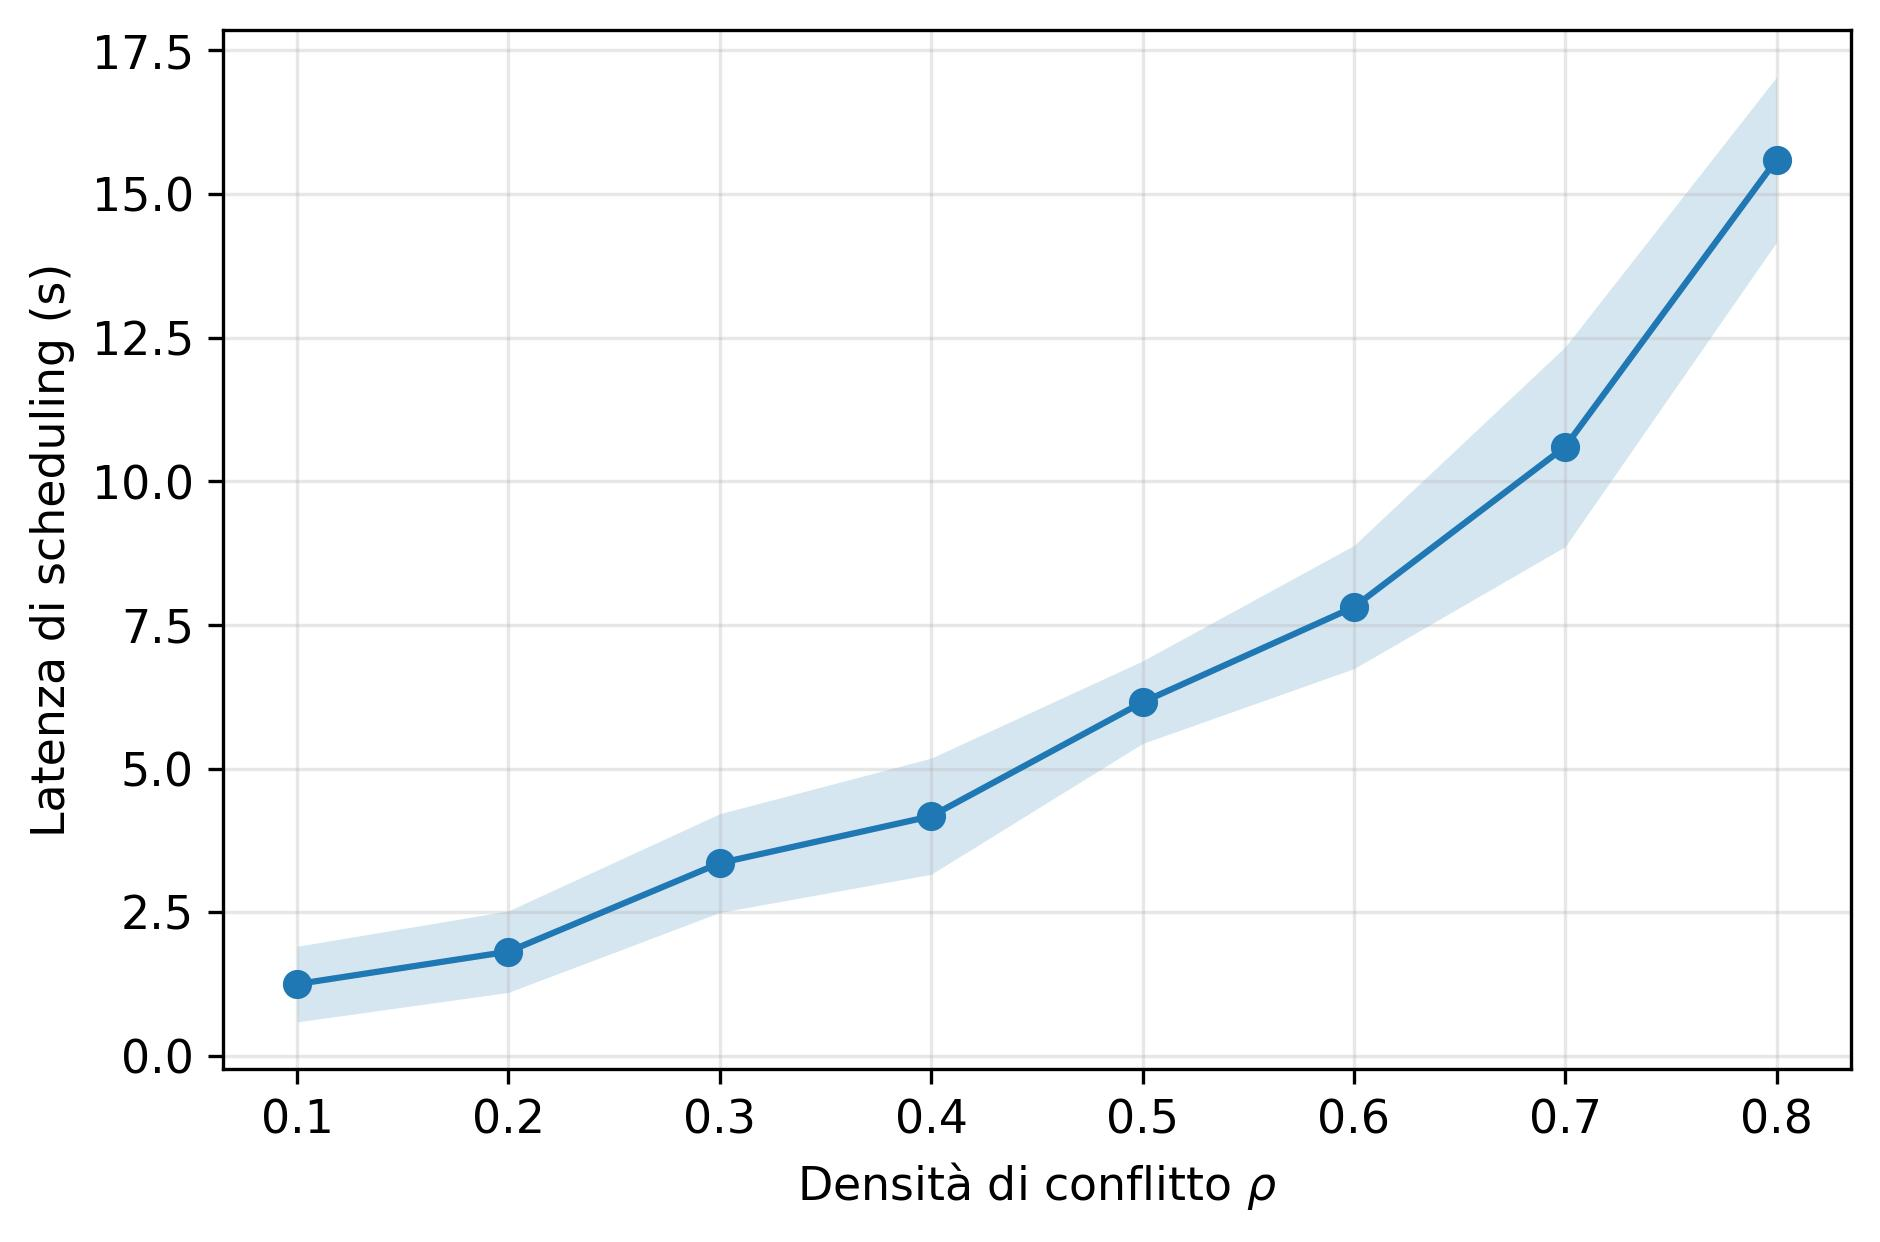
\includegraphics[width=\textwidth]{immagini/val_conflitti/conflicts_latenza.jpg}
        \caption{Latenza media di scheduling.}
        \label{fig:conflitti-latenza}
    \end{subfigure}
    \hfill
    \begin{subfigure}[b]{0.48\textwidth}
        \centering
        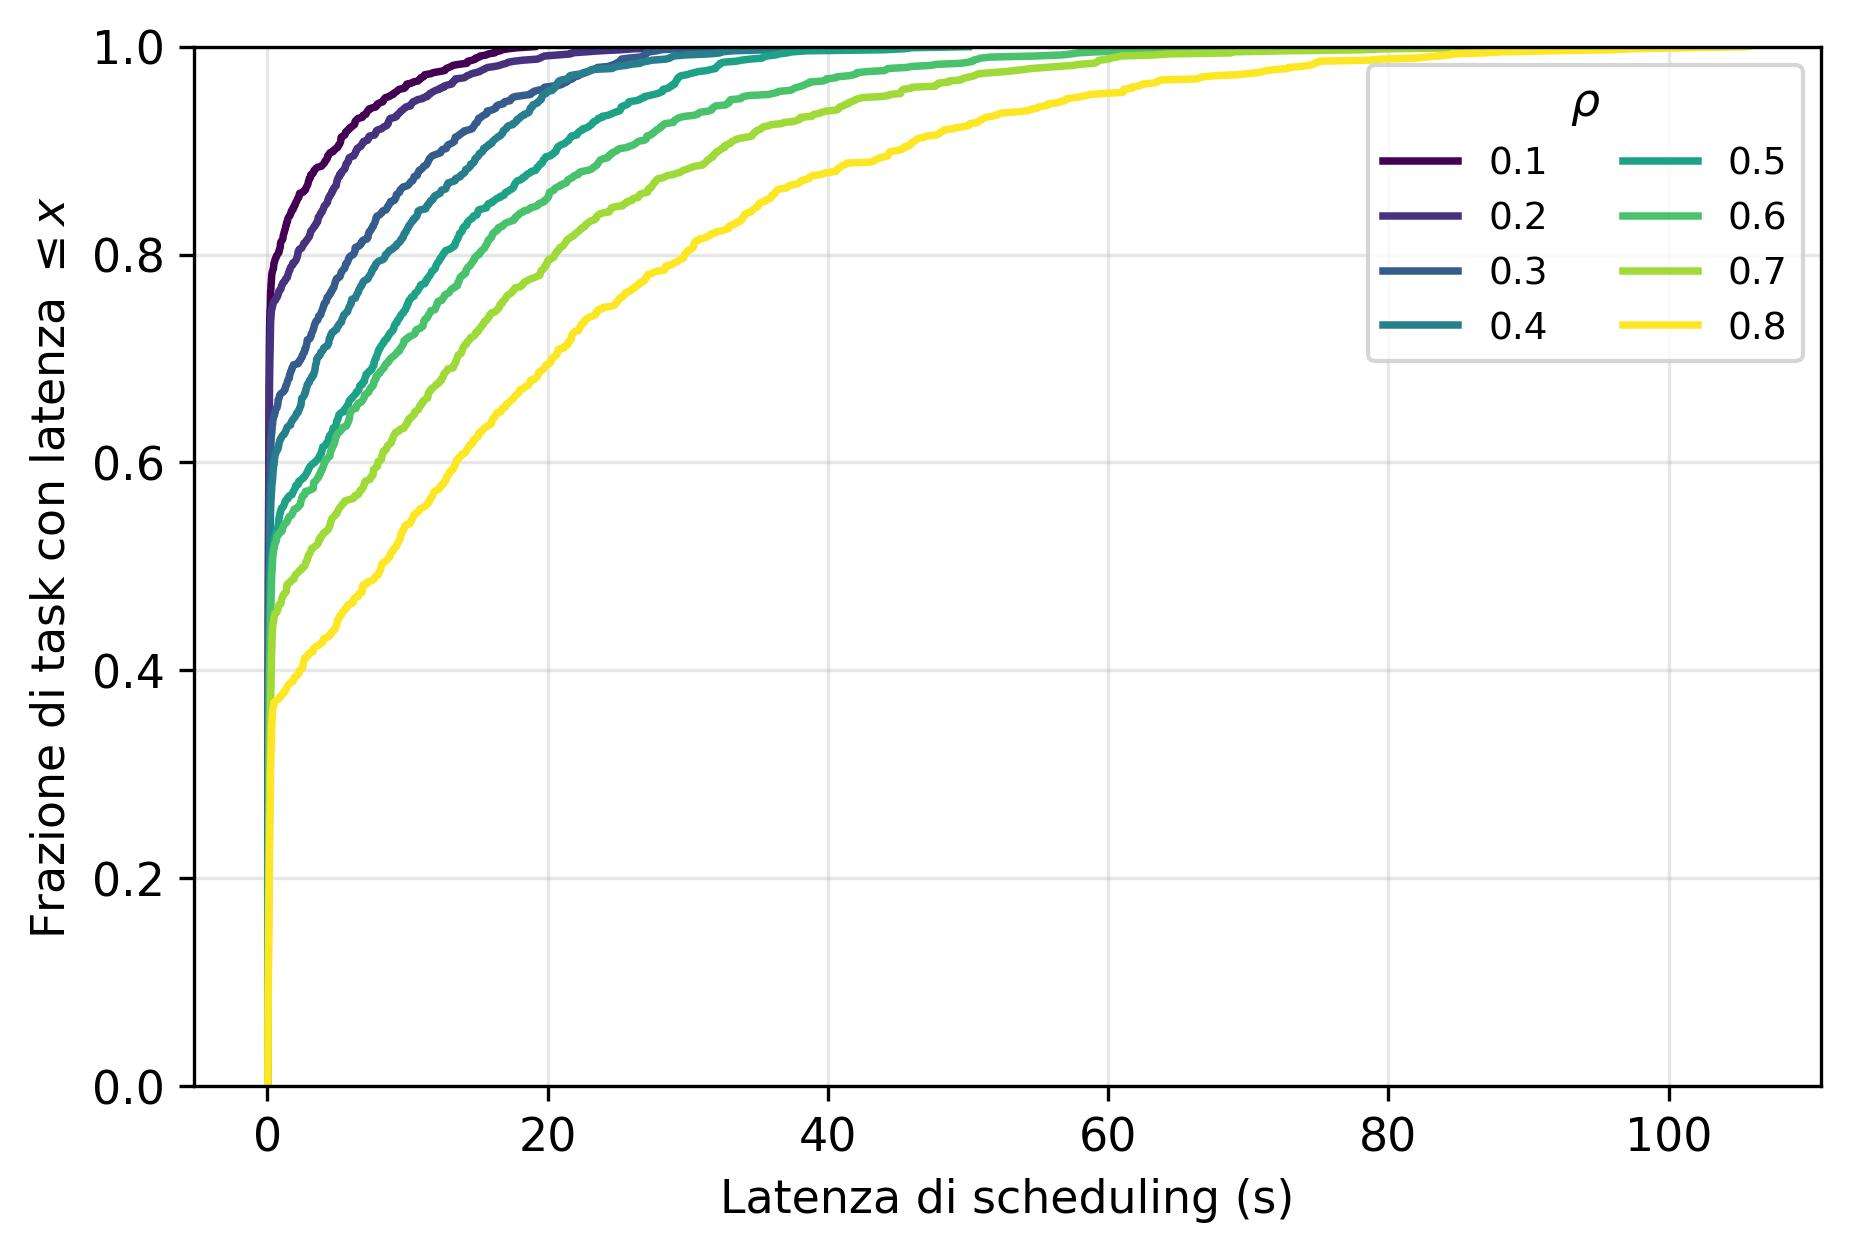
\includegraphics[width=\textwidth]{immagini/val_conflitti/conflicts_cdf.jpg}
        \caption{Distribuzione cumulata della latenza.}
        \label{fig:conflitti-cdf}
    \end{subfigure}
    \caption{Latenza di scheduling al variare della densità di conflitto $\rho$.}
    \label{fig:conflitti-latenza-cdf}
\end{figure}

Il primo effetto da osservare è quello sulla latenza di scheduling, mostrata nella Figura~\ref{fig:conflitti-latenza-cdf} sia come media tra le repliche sia come distribuzione cumulata. La latenza media cresce in modo monotono lungo tutta la griglia, da circa 1.2 secondi a $\rho = 0.1$ fino a 15.6 secondi a $\rho = 0.8$, con una crescita che si fa più ripida alle densità alte. L'andamento è coerente con l'aspettativa formulata nella Sezione~\ref{subsec:perimetro_valutazione} ed è confermato dai test statistici condotti sulle latenze medie delle singole repliche. Il test di Kruskal–Wallis indica che la densità ha un effetto significativo sulla latenza ($H = 37.08$, $p < 10^{-5}$), e la correlazione di Spearman tra densità e latenza conferma che la crescita è monotona e sistematica su tutta la griglia e non frutto di oscillazioni casuali ($r_s = 0.97$, $p < 10^{-24}$). La distribuzione cumulata nella stessa figura mostra la stessa crescita vista dall'intera popolazione dei task. Ogni curva sale rapidamente vicino all'origine, dove si trovano i task schedulati quasi subito, per poi distendersi in una coda che raccoglie i task in attesa di sanificazione. Al crescere di $\rho$ il tratto iniziale si abbassa, perché una quota minore di task passa senza attese, e la coda si allunga verso destra, perché chi viene bloccato attende di più. 

\begin{figure}[htb]
    \centering
    \begin{subfigure}[b]{0.48\textwidth}
        \centering
        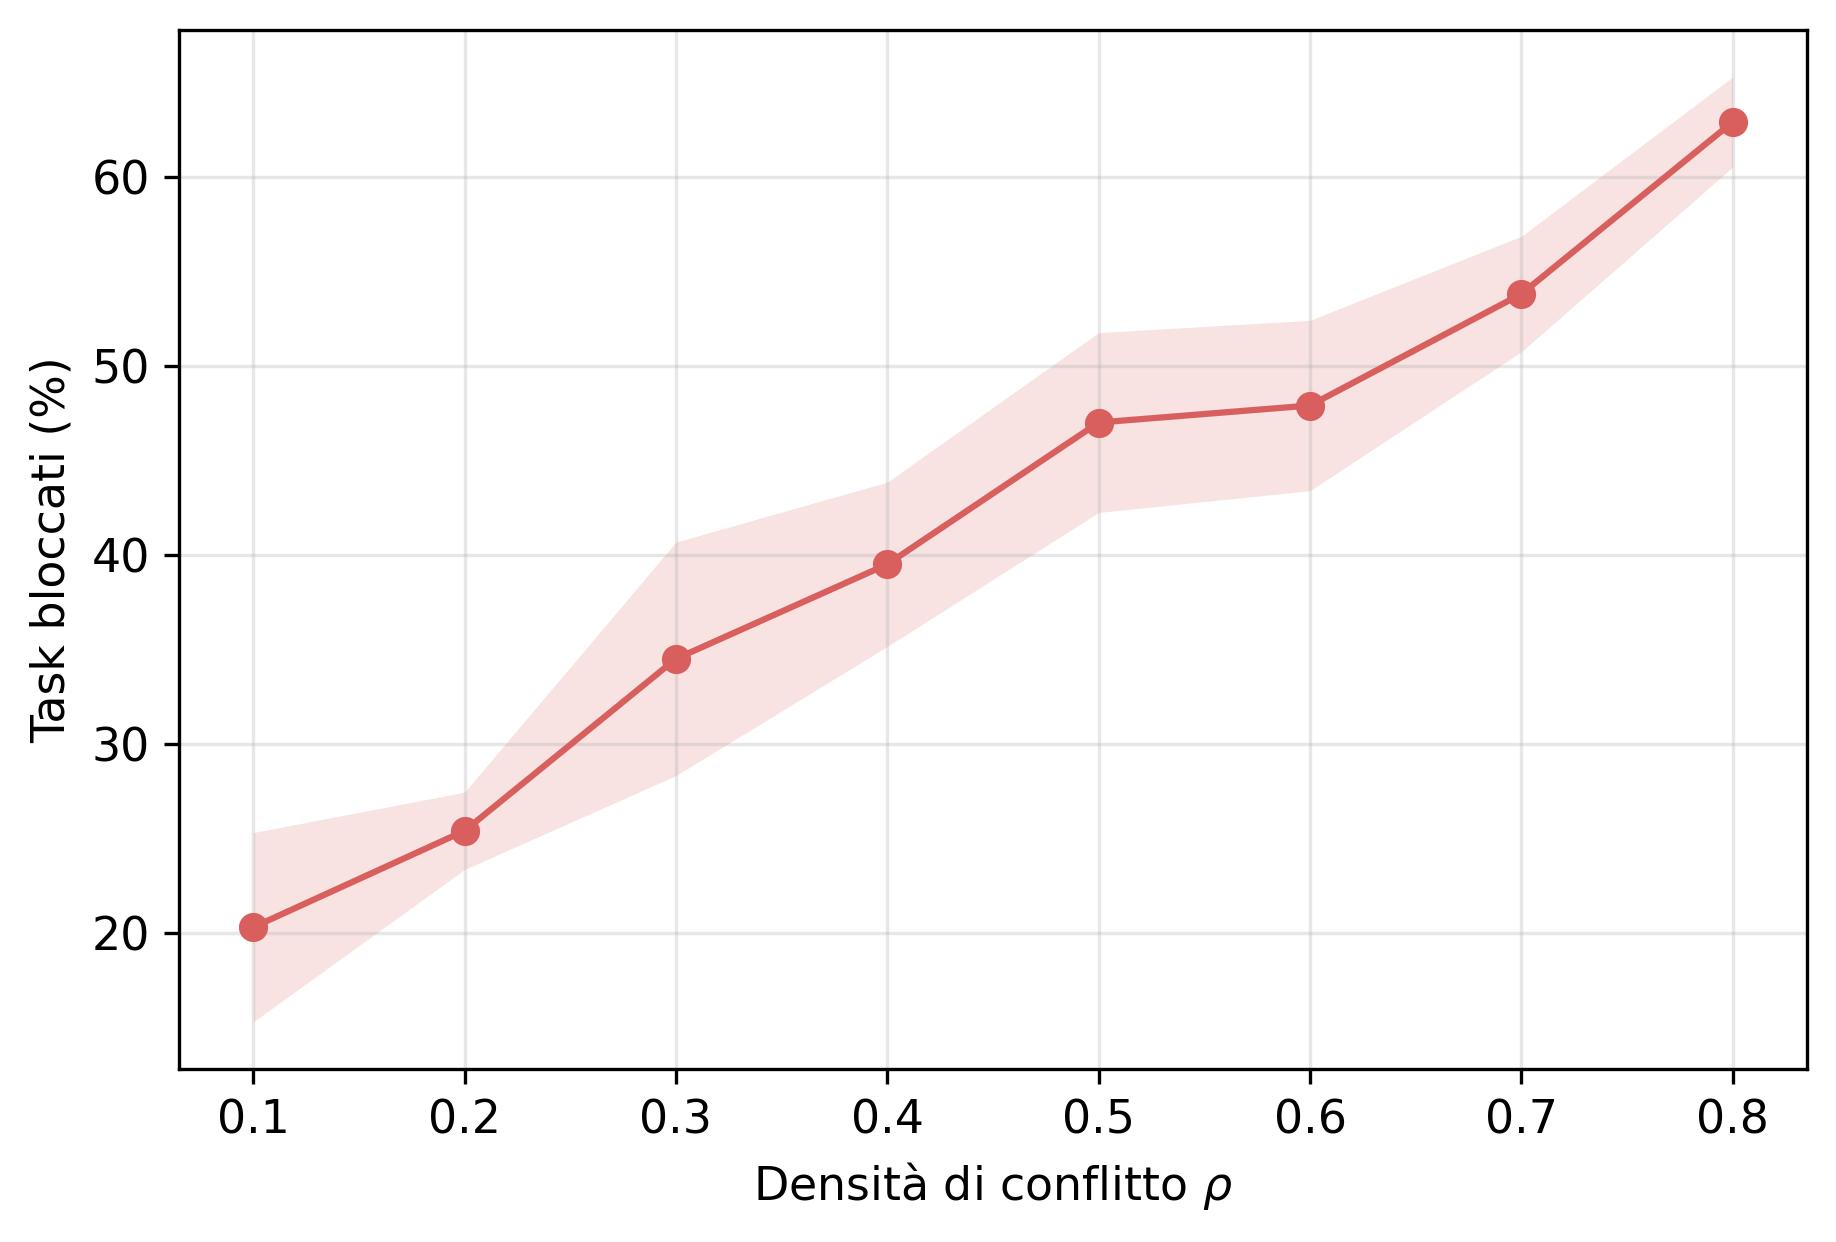
\includegraphics[width=\textwidth]{immagini/val_conflitti/conflicts_bloccati.jpg}
        \caption{Frazione di task bloccati.}
        \label{fig:conflitti-bloccati}
    \end{subfigure}
    \hfill
    \begin{subfigure}[b]{0.48\textwidth}
        \centering
        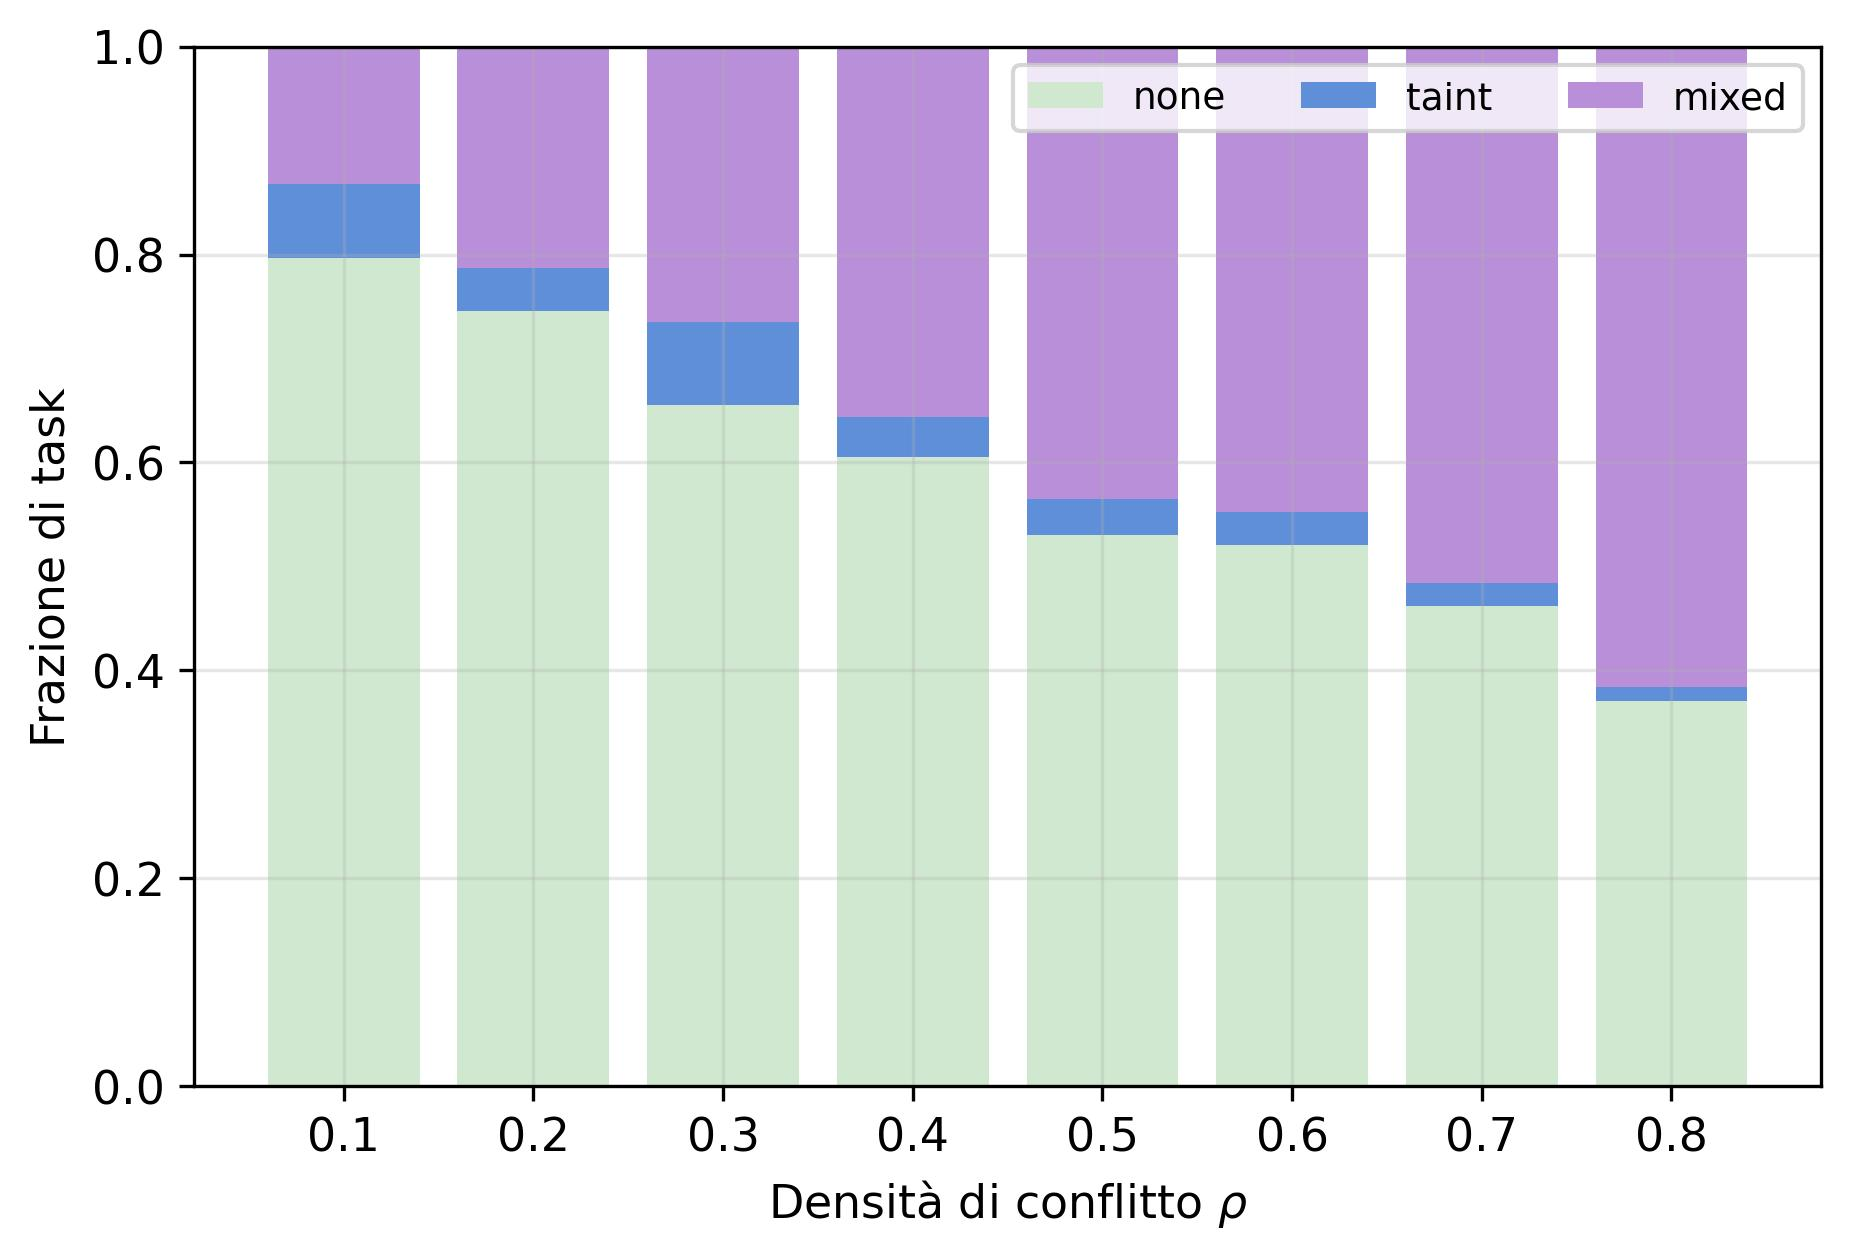
\includegraphics[width=\textwidth]{immagini/val_conflitti/conflicts_cause_blocco.jpg}
        \caption{Ripartizione dei task per causa di blocco.}
        \label{fig:conflitti-cause}
    \end{subfigure}
    \caption{Blocco dei task al variare della densità di conflitto $\rho$.}
    \label{fig:conflitti-bloccati-cause}
\end{figure}

La crescita osservata è riconducibile alla frazione di task bloccati, cioè respinti almeno una volta prima di essere assegnati, che cresce regolarmente dal 20\% a $\rho = 0.1$ fino al 63\% a $\rho = 0.8$, come mostra la Figura~\ref{fig:conflitti-bloccati-cause}. 
È su questa grandezza che la densità di conflitto agisce direttamente, dato che la densità non allunga di per sé l'attesa di un singolo task, ma rende più probabile che un task venga bloccato e debba quindi attendere un nuovo tentativo di assegnazione.

Di fianco, la ripartizione per causa distingue tutti i task della run in base a ciò che hanno incontrato prima di essere assegnati. La quota segnata come \emph{none} raccoglie i task assegnati al primo tentativo, senza alcun blocco; quella segnata come \emph{taint} i task esclusi perché il nodo era in sanificazione, e quella marcata come \emph{mixed} i task che nel corso della loro attesa hanno incontrato sia una traccia in conflitto sia la procedura di sanificazione. Gli ultimi due casi sono in realtà due facce dello stesso fenomeno, perché la traccia contestuale che blocca un task viene rimossa proprio dalla sanificazione del nodo, e durante quella finestra il nodo resta escluso per via del \emph{taint}. Per questo un task che attende la pulizia di un nodo attraversa quasi sempre entrambe le cause e ricade in \emph{mixed}, mentre i blocchi dovuti al solo \emph{taint} restano una quota minore. Ciò che conta, ai fini dell'esperimento, è che i task bloccati solamente dal \emph{taint} non crescono con $\rho$, ma restano una quota contenuta che tende anzi a ridursi, dato che l'intervallo $\tau$ è fisso. Quindi, a crescere è soltanto il blocco dovuto alle tracce in conflitto, confermando che l'aumento di latenza dipende solamente dai conflitti e non dalla sanificazione, che in questo caso è costante.

\begin{figure}[htb]
    \centering
    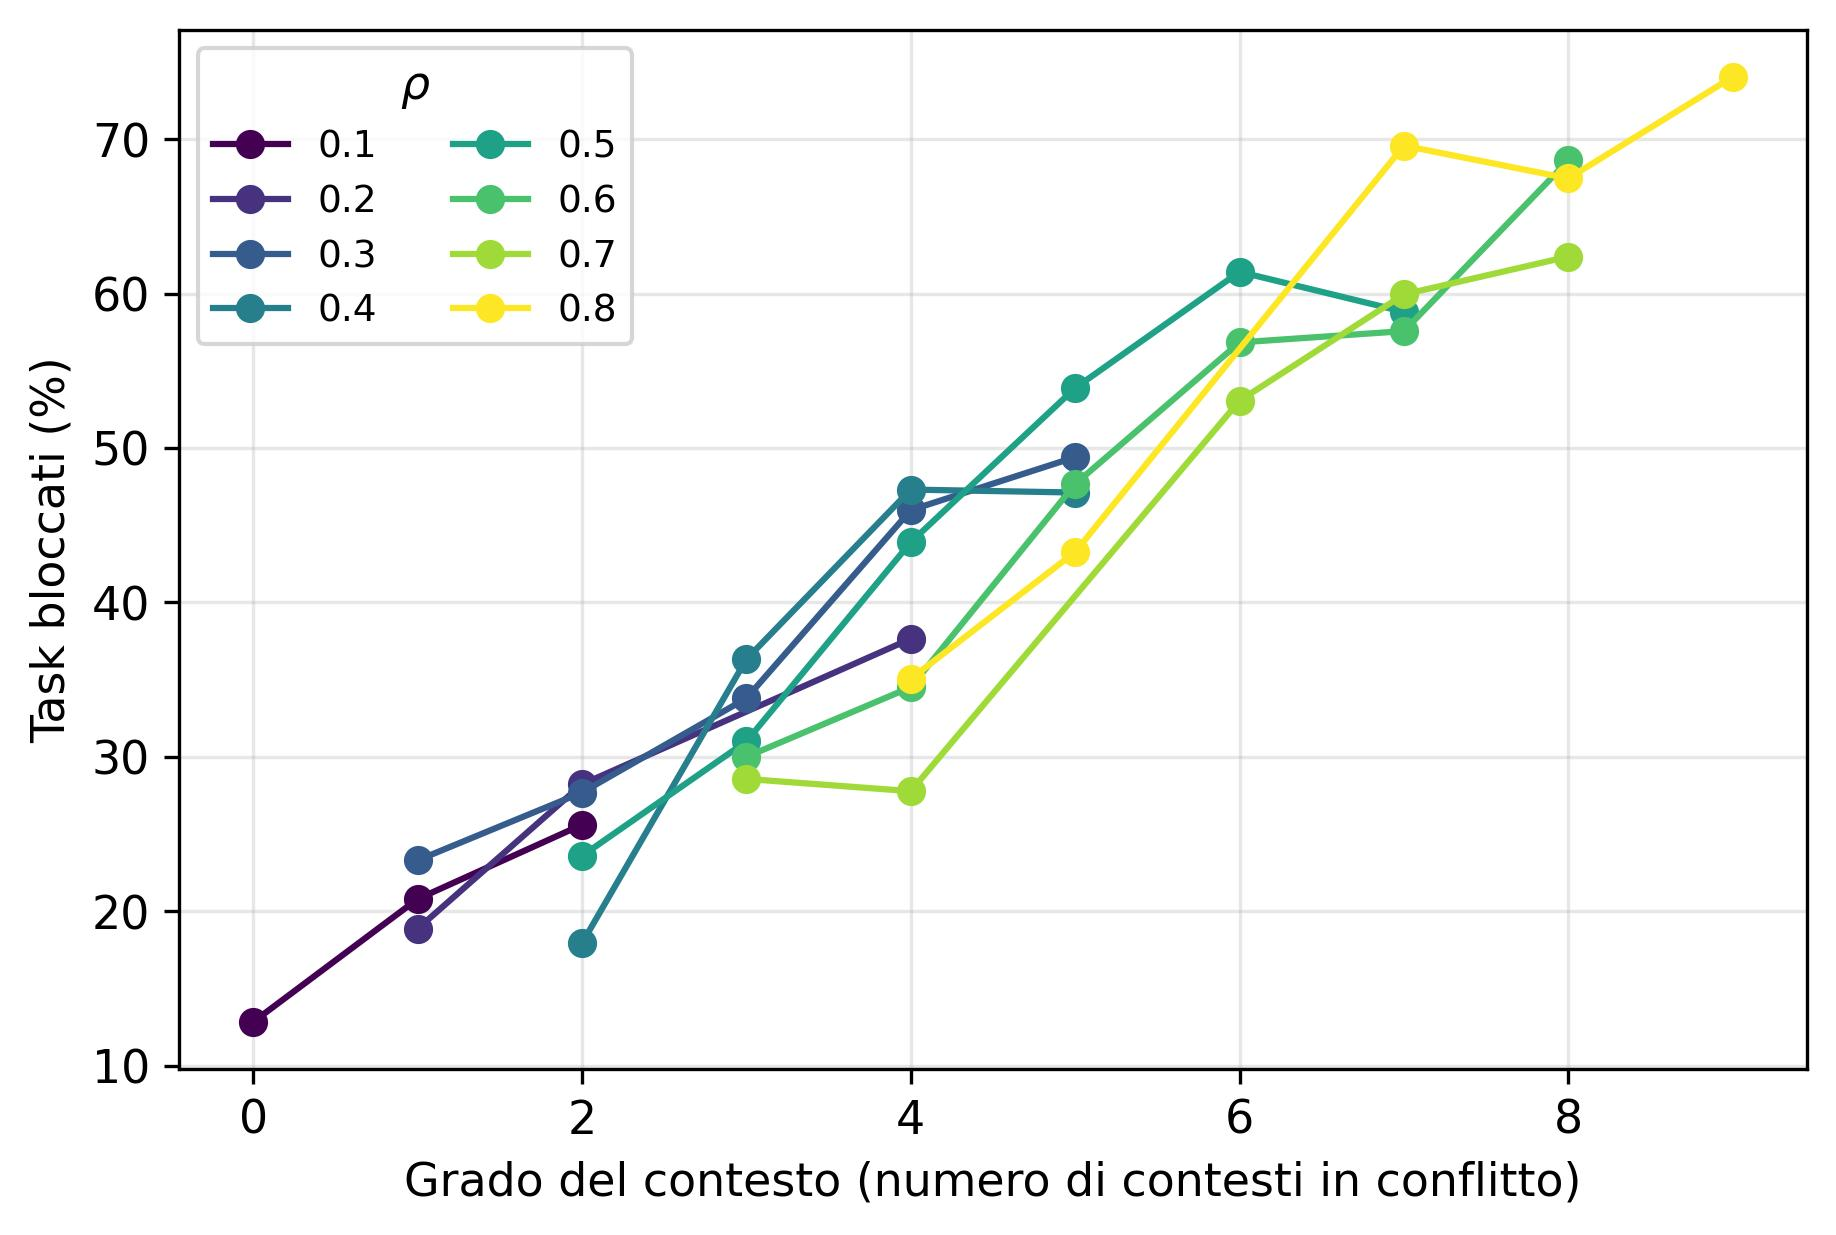
\includegraphics[width=0.48\textwidth]{immagini/val_conflitti/conflicts_grado.jpg}
    \caption{Frazione di task bloccati in funzione del grado del contesto.}
    \label{fig:conflitti-grado}
\end{figure}

Resta da capire perché sia la densità a far salire il numero di blocchi, e la Figura~\ref{fig:conflitti-grado} lo chiarisce riportando la frazione di task bloccati in funzione del grado del contesto richiesto. Le curve delle diverse densità tendono a sovrapporsi lungo un'unica tendenza comune, dato che a parità di grado un task viene bloccato con la stessa frequenza qualunque sia la densità dello scenario. Il blocco non dipende quindi dalla densità in sé, ma dal grado del contesto del task, e la densità agisce sulla latenza proprio perché, aumentando, fa salire il grado medio dei contesti.

\begin{figure}[htb]
    \centering
    \begin{subfigure}[b]{0.48\textwidth}
        \centering
        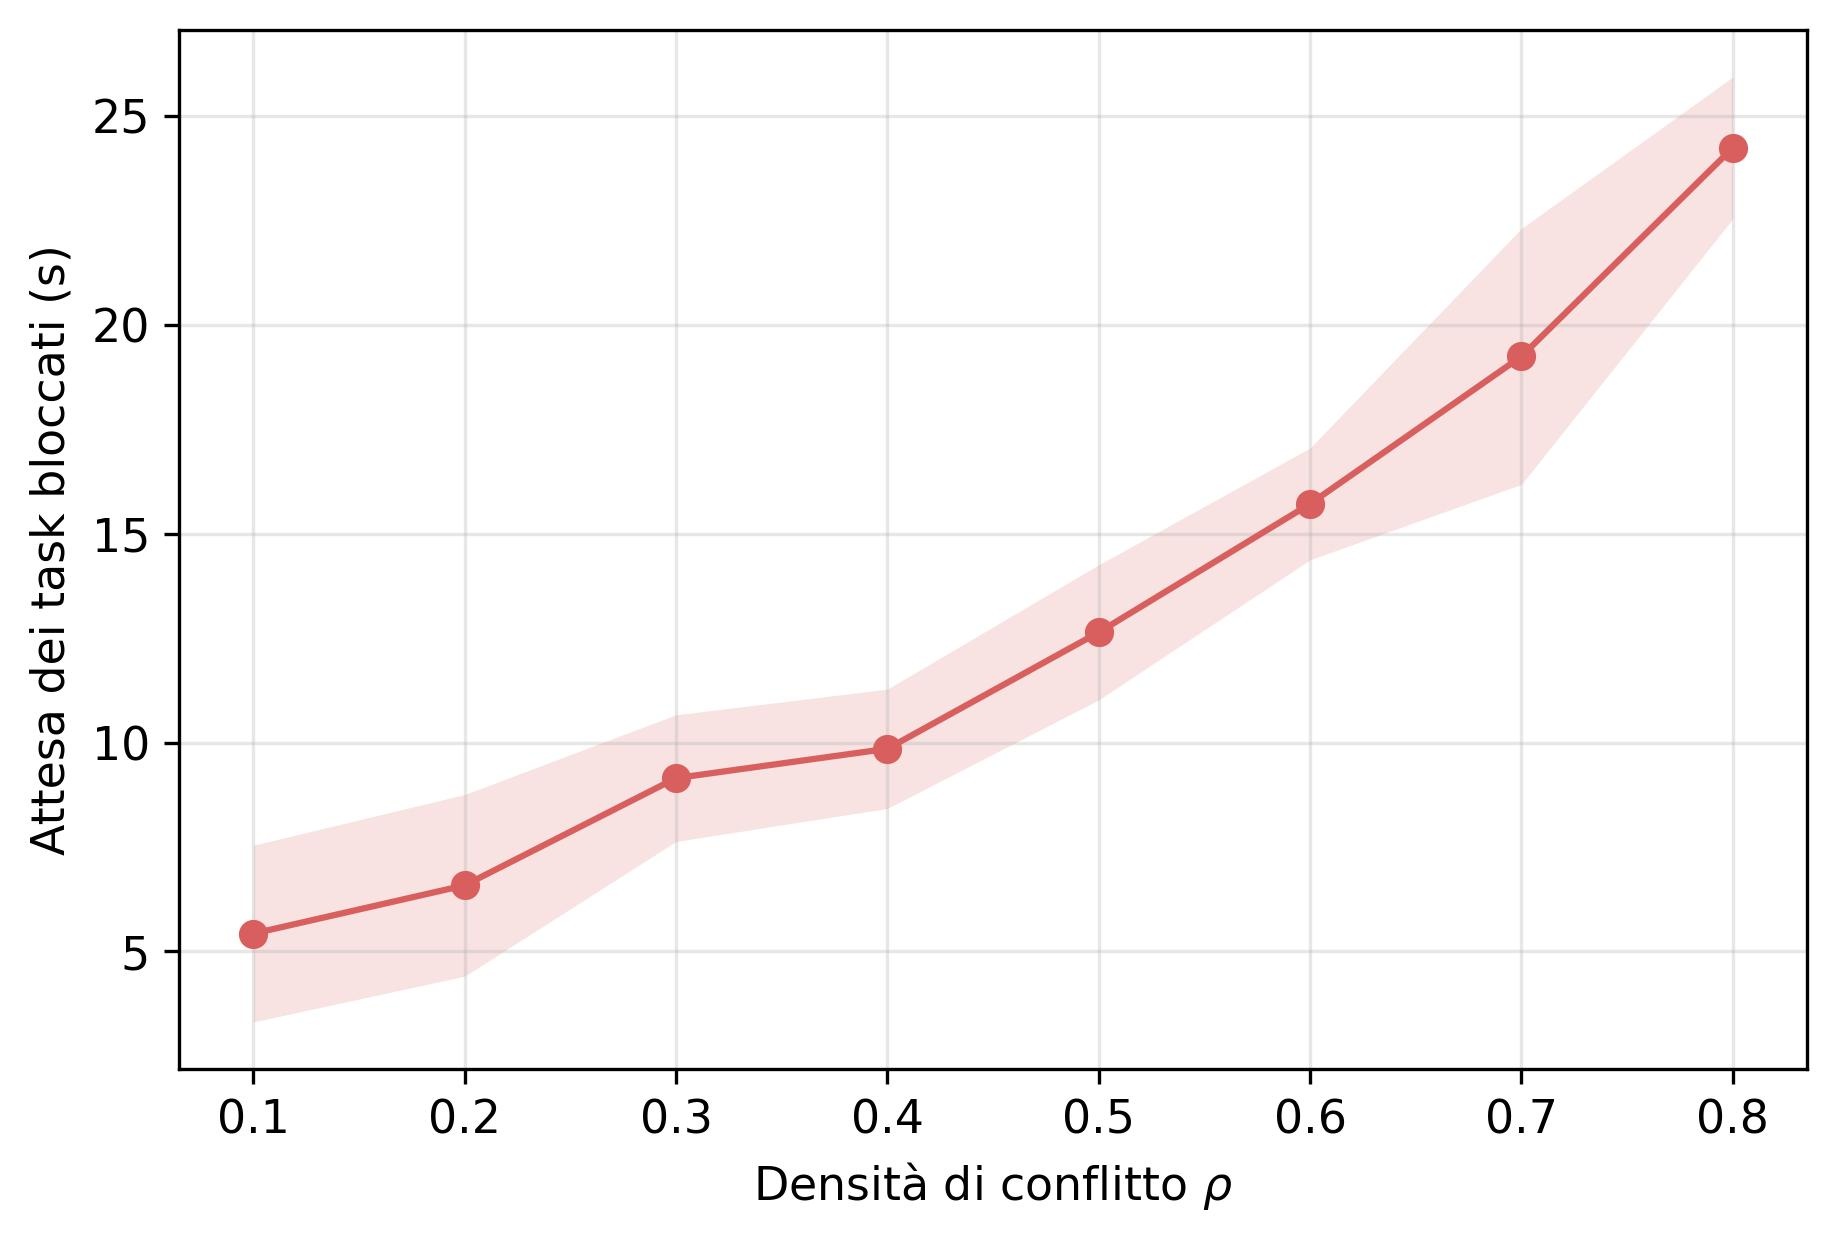
\includegraphics[width=\textwidth]{immagini/val_conflitti/conflicts_attesa.jpg}
        \caption{Attesa media dei task bloccati.}
        \label{fig:conflitti-attesa}
    \end{subfigure}
    \hfill
    \begin{subfigure}[b]{0.48\textwidth}
        \centering
        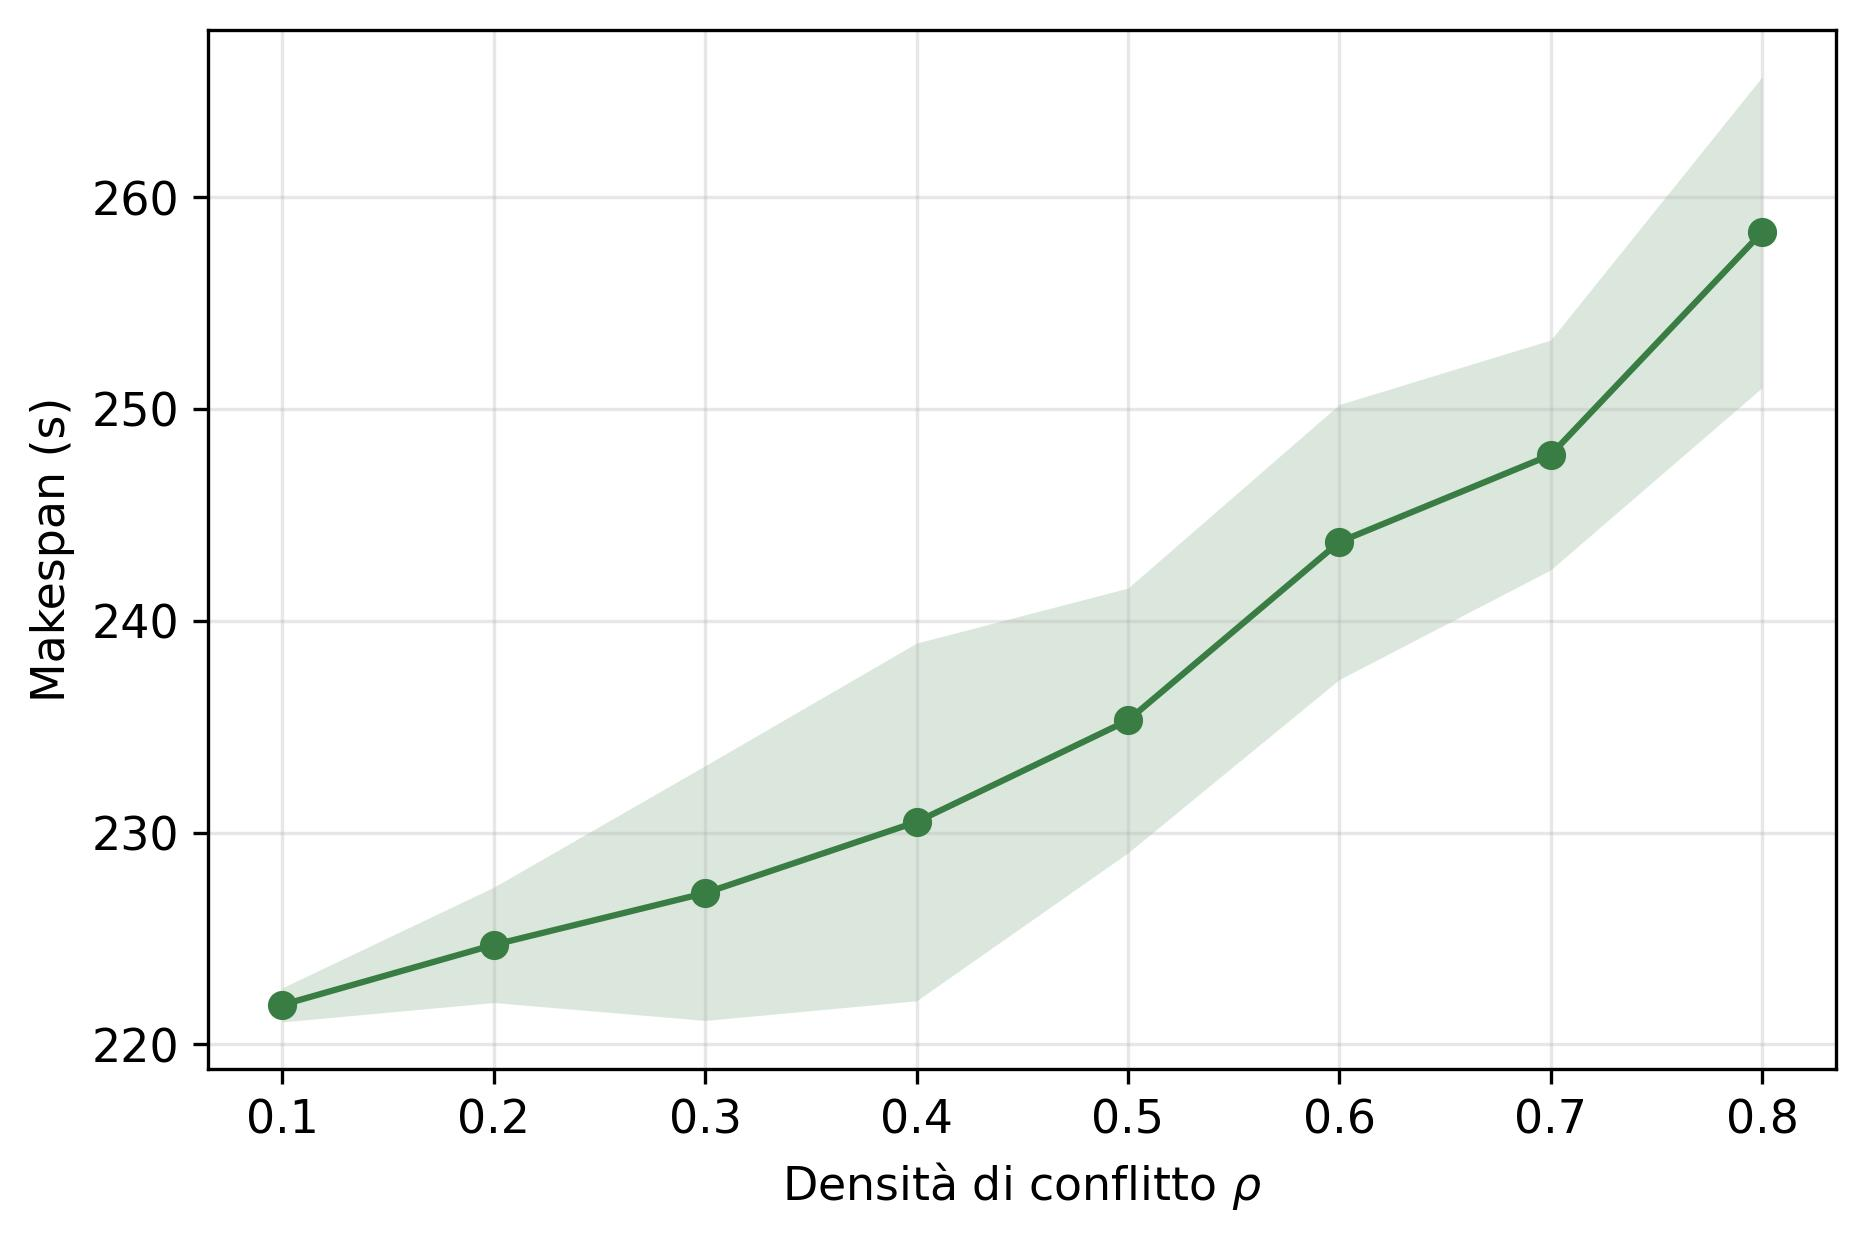
\includegraphics[width=\textwidth]{immagini/val_conflitti/conflicts_makespan.jpg}
        \caption{Makespan del batch.}
        \label{fig:conflitti-makespan}
    \end{subfigure}
    \caption{Costo globale dei conflitti al variare della densità $\rho$.}
    \label{fig:conflitti-attesa-makespan}
\end{figure}

Oltre alla probabilità di blocco, i conflitti incidono anche sul tempo, che la Figura~\ref{fig:conflitti-attesa-makespan} mostra da due prospettive diverse. L'attesa media dei task bloccati, dal primo rifiuto fino al binding, cresce da circa 5 secondi a $\rho = 0.1$ fino a oltre 24 secondi a $\rho = 0.8$: a densità più alta un task bloccato trova contaminati più nodi e deve attendere che un numero maggiore di essi venga ripulito prima di trovarne uno compatibile. Il makespan, ovvero il tempo per completare l'intero batch di 200 task, cresce anch'esso ma molto più lentamente, da circa 222 a 258 secondi, perché include per costruzione i 200 secondi di sottomissione e perché le attese dei task bloccati si sovrappongono nel tempo invece di sommarsi, dato che molti task attendono lo stesso ciclo di sanificazione. Le due viste restano entrambe utili, perché la prima misura il costo percepito da chi sottomette e la seconda quello complessivo sostenuto dal cluster.

Nel complesso, l'esperimento conferma che la latenza di scheduling cresce in modo monotono e significativo con la densità di conflitto, e individua nel grado dei singoli contesti, più che nella densità complessiva, la grandezza che governa il fenomeno.

% ------------------------------------------------------------ %

\section{Impatto dell'Intervallo di Sanificazione}
\label{sec:impatto_intervallo}

Il secondo esperimento fa variare l'intervallo di sanificazione $\tau$ tra 1 e 50 secondi mantenendo fissa la densità di conflitto a $\rho = 0.5$, un valore intermedio che garantisce una quota di task bloccati sufficiente a rendere osservabile l'effetto della sanificazione senza saturare il sistema. A differenza della densità di conflitto, che agisce sulla probabilità di blocco, l'intervallo agisce sul tempo che un task bloccato attende prima di potersi schedulare, e il suo effetto non è monotono.

\begin{figure}[htb]
    \centering
    \begin{subfigure}[b]{0.48\textwidth}
        \centering
        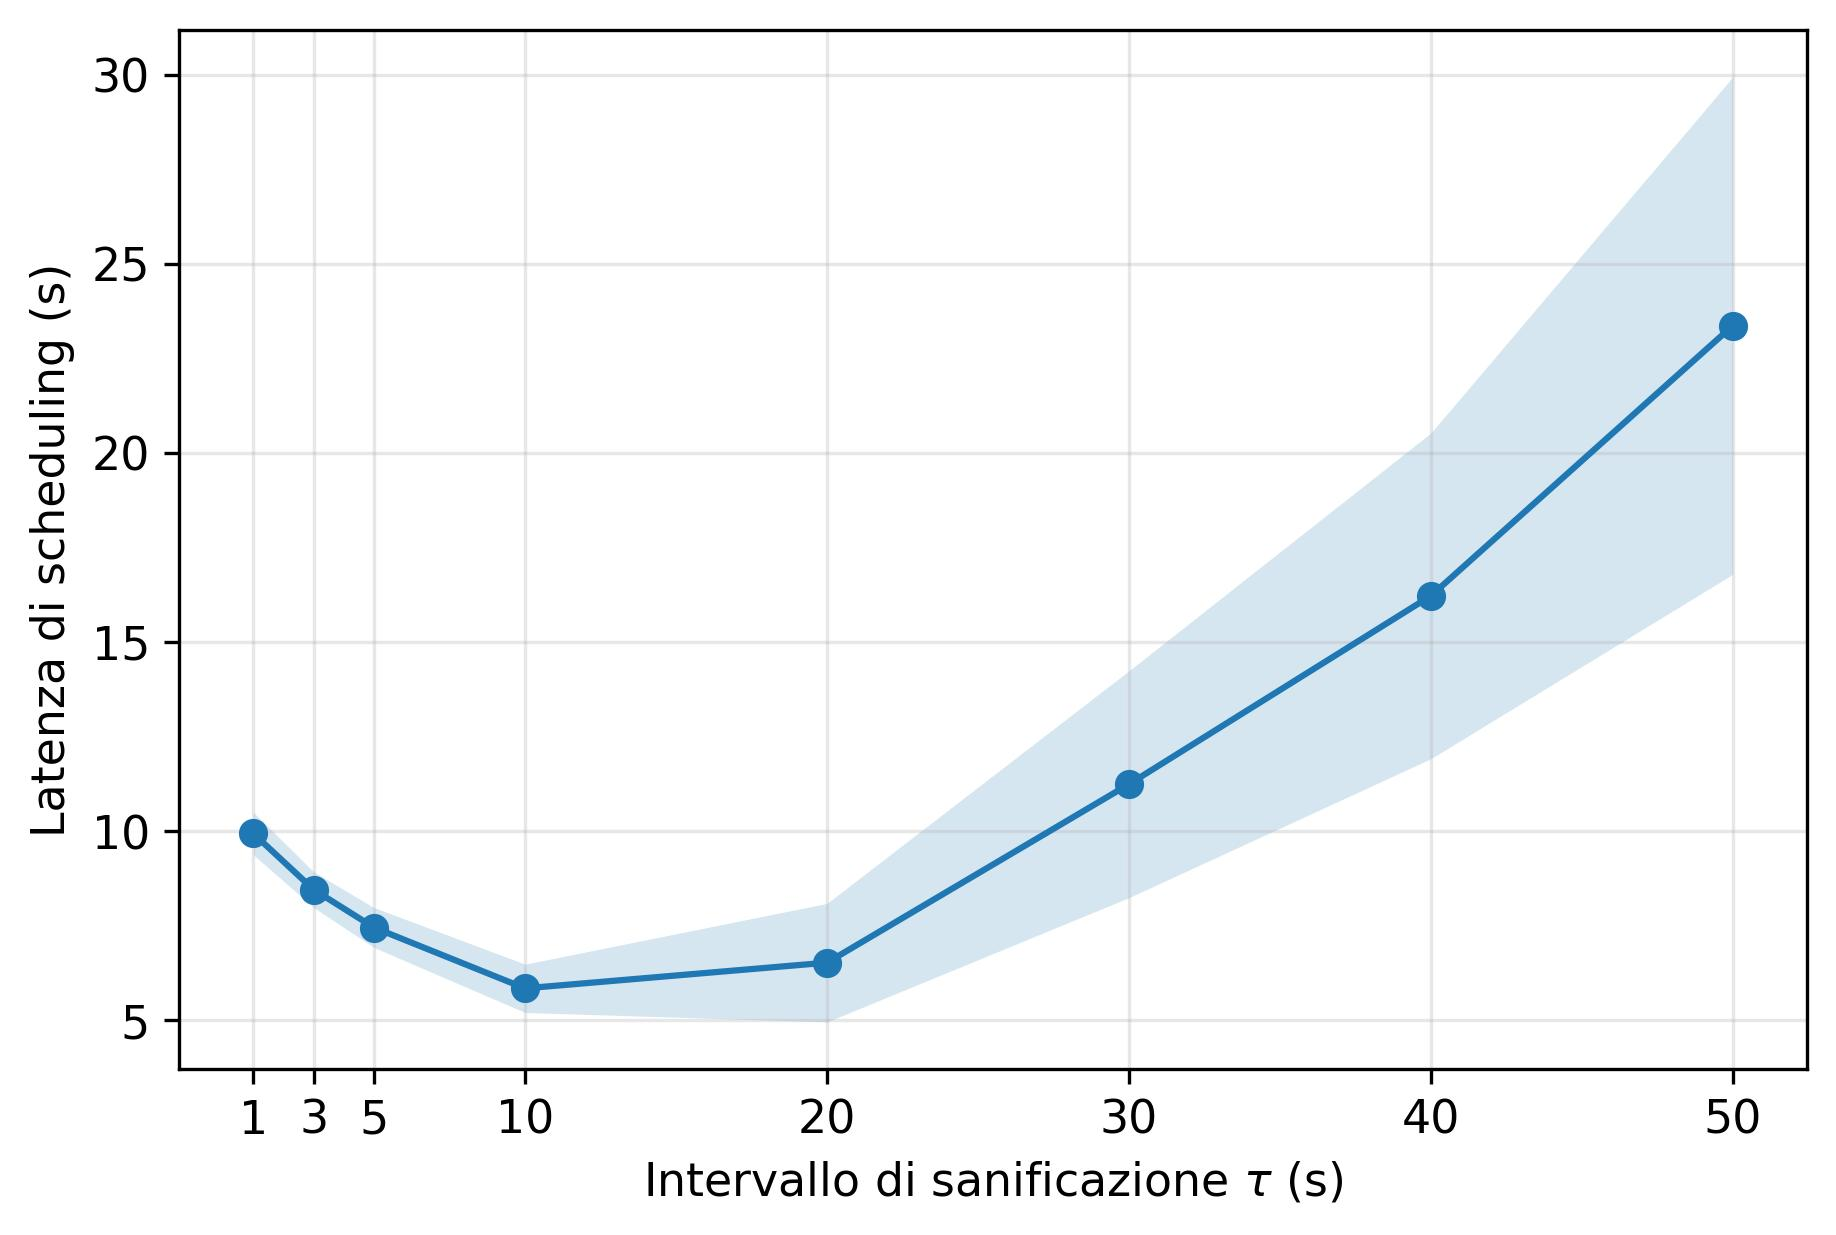
\includegraphics[width=\textwidth]{immagini/val_sanificazione/sanitize_latenza.jpg}
        \caption{Latenza media di scheduling.}
        \label{fig:sanificazione-latenza}
    \end{subfigure}
    \hfill
    \begin{subfigure}[b]{0.48\textwidth}
        \centering
        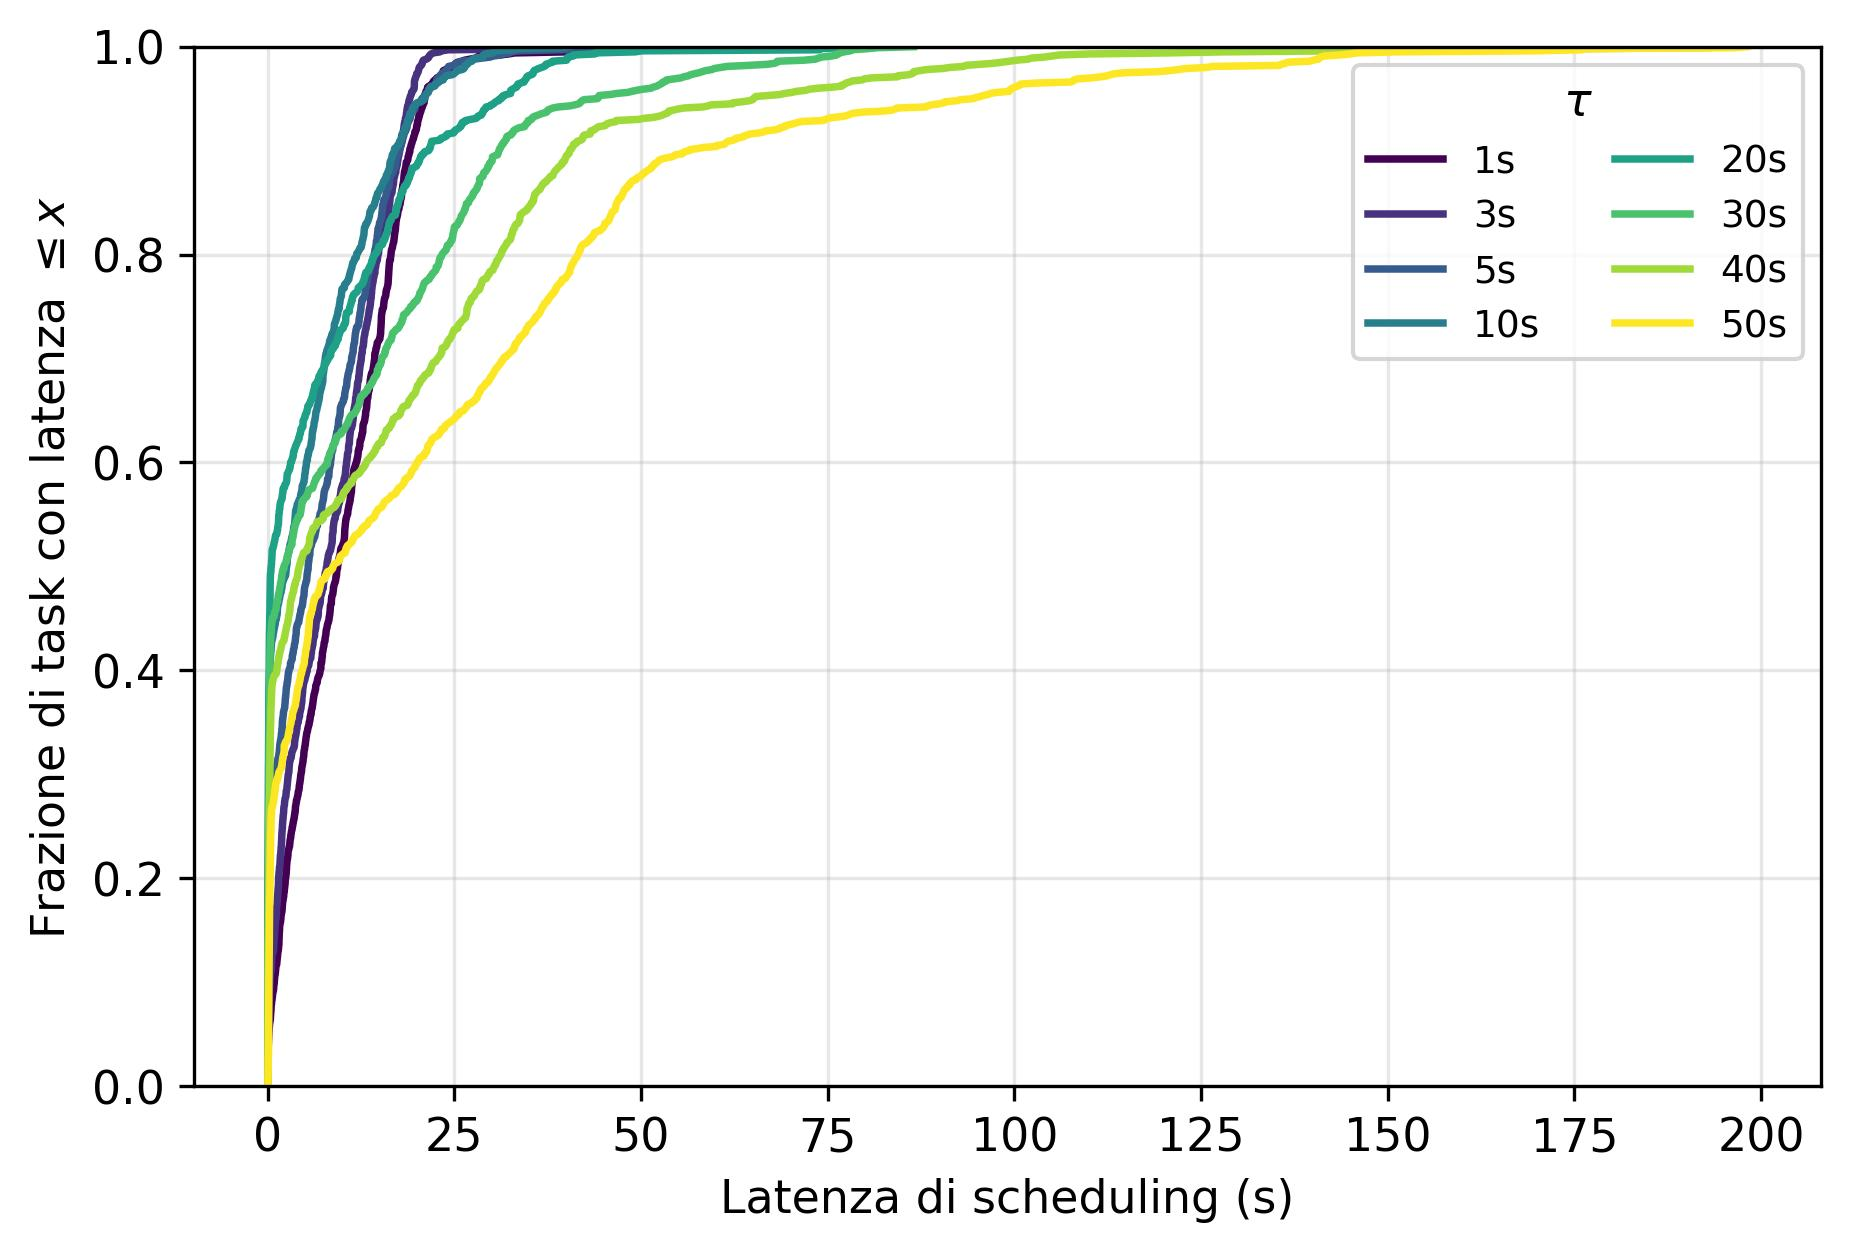
\includegraphics[width=\textwidth]{immagini/val_sanificazione/sanitize_cdf.jpg}
        \caption{Distribuzione cumulata della latenza.}
        \label{fig:sanificazione-cdf}
    \end{subfigure}
    \caption{Latenza di scheduling al variare dell'intervallo di sanificazione $\tau$.}
    \label{fig:sanificazione-latenza-cdf}
\end{figure}

La latenza di scheduling, mostrata nella Figura~\ref{fig:sanificazione-latenza-cdf}, conferma l'andamento a U anticipato nella Sezione~\ref{subsec:perimetro_valutazione}. Partendo da circa 10 secondi a $\tau = 1$, la latenza media scende fino a un minimo di 5.8 secondi a $\tau = 10$, per poi risalire e raggiungere oltre 23 secondi a $\tau = 50$. I due bracci della curva hanno origini diverse, discusse più avanti, ma la loro esistenza suggerisce che né sanificare molto spesso né sanificare molto di rado sia la scelta migliore. Un altro aspetto che la curva rende evidente è l'allargarsi della varianza verso destra, perché agli intervalli più lunghi una run contiene pochi cicli di sanificazione e la latenza dipende sempre più da quando esattamente questi cicli cadono rispetto ai task in esecuzione, rendendo la misura meno stabile. Il test di Kruskal–Wallis conferma che l'intervallo ha un effetto significativo sulla latenza ($H = 31.87$, $p < 10^{-4}$), mentre la natura del minimo emerge dai confronti a coppie tra valori adiacenti di $\tau$, condotti con il test di Mann–Whitney a due code sulle latenze medie delle singole repliche. La latenza a $\tau = 10$ risulta significativamente inferiore a quella a $\tau = 5$ ($U = 0$, $p < 10^{-2}$) ma non è distinguibile da quella a $\tau = 20$ ($U = 9$, $p = 0.90$), che a sua volta è inferiore a quella a $\tau = 30$ ($U = 1$, $p = 0.03$). L'ottimo non è quindi un singolo valore, ma una regione compresa tra $\tau = 10$ e $\tau = 20$, ai cui estremi le prestazioni non risultano statisticamente distinguibili. La distribuzione cumulata mostra lo stesso andamento dal punto di vista dei singoli task. Agli intervalli brevi il tratto iniziale è basso, perché pochi task trovano un nodo disponibile al primo tentativo, ma la coda è corta, perché i nodi tornano disponibili in fretta. Tra $\tau = 10$ e $\tau = 20$ il tratto iniziale raggiunge la sua altezza massima, mentre agli intervalli lunghi si abbassa di nuovo e la coda si allunga verso destra, fino a superare gli 80 secondi a $\tau = 50$.

\begin{figure}[htb]
    \centering
    \begin{subfigure}[b]{0.48\textwidth}
        \centering
        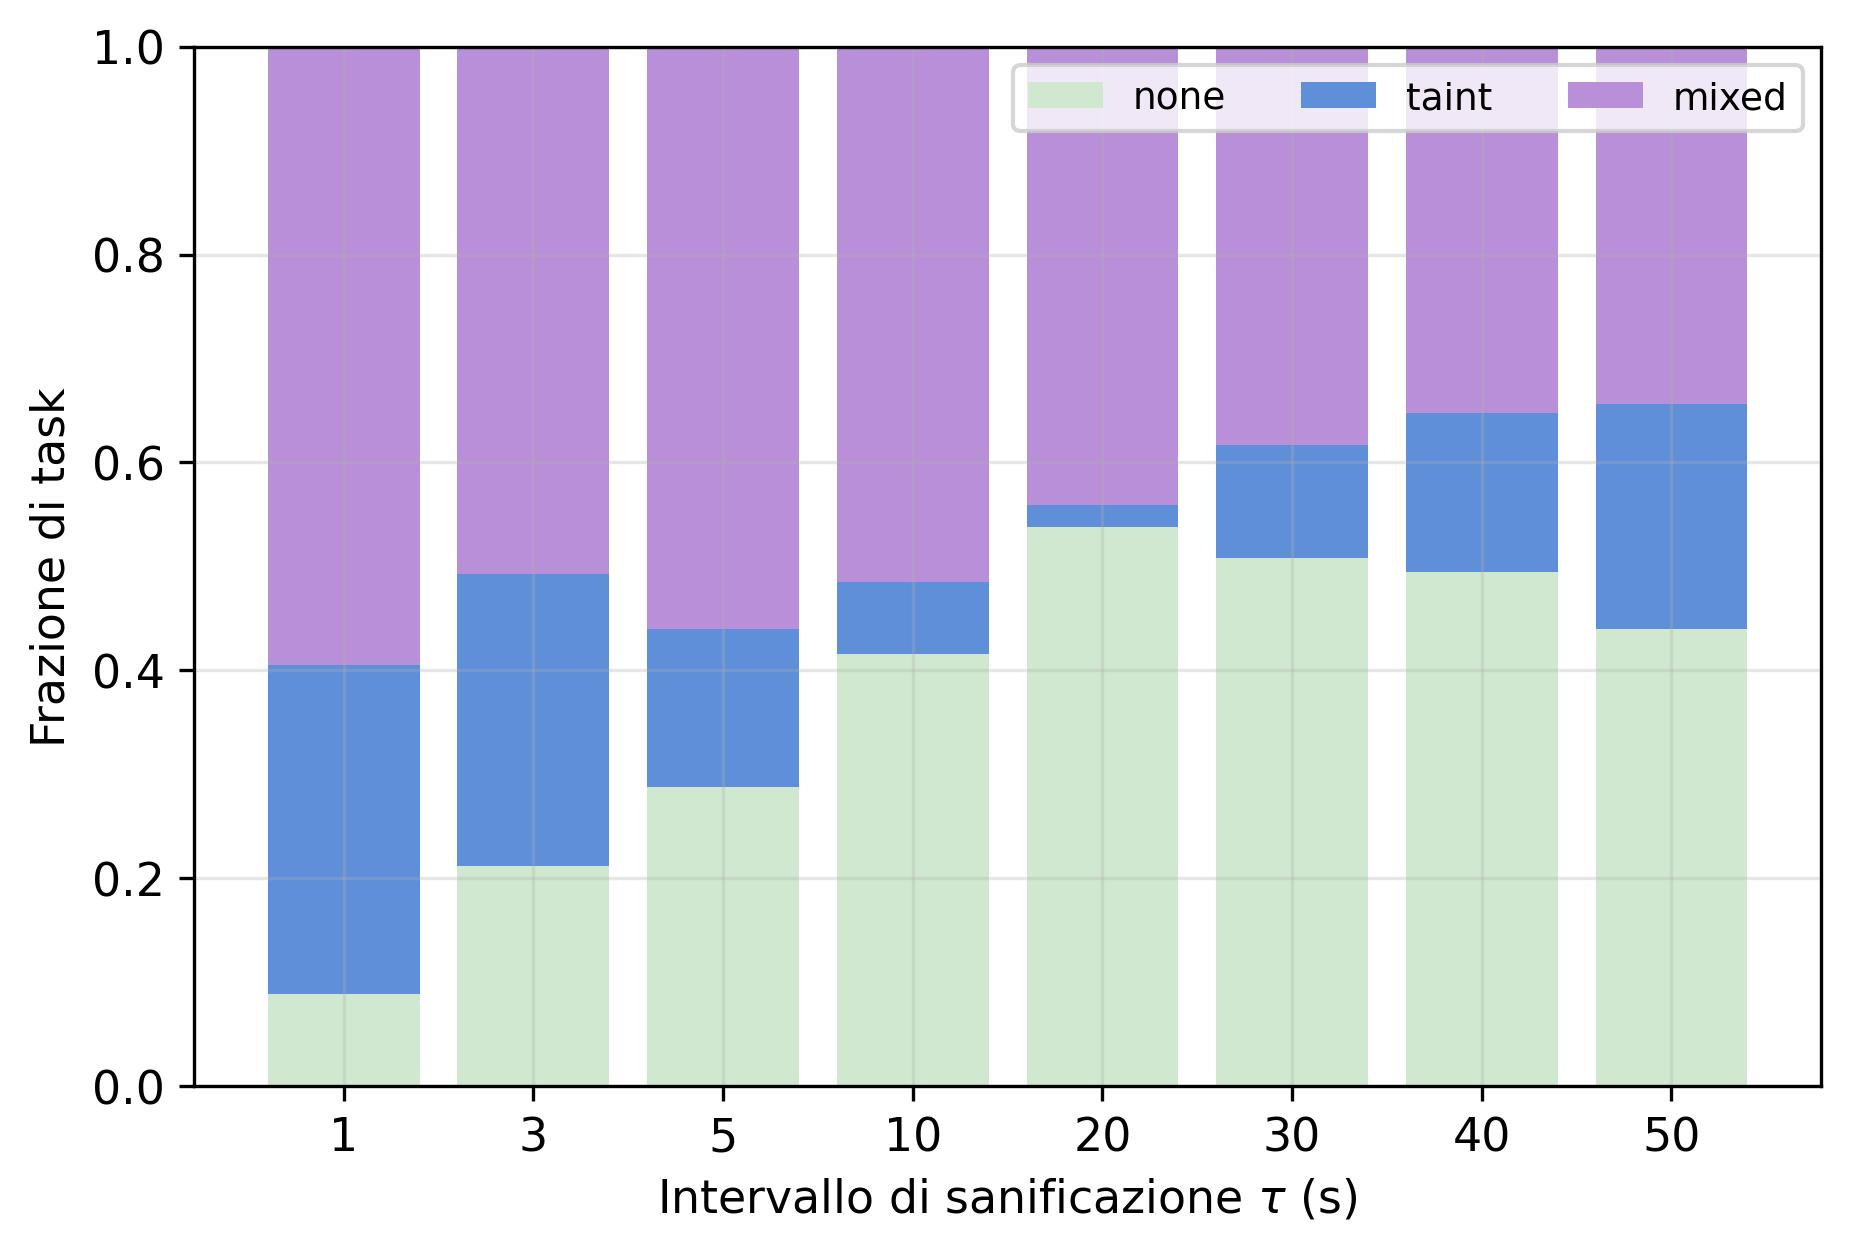
\includegraphics[width=\textwidth]{immagini/val_sanificazione/sanitize_cause_blocco.jpg}
        \caption{Ripartizione dei task per causa di blocco.}
        \label{fig:sanificazione-cause}
    \end{subfigure}
    \hfill
    \begin{subfigure}[b]{0.48\textwidth}
        \centering
        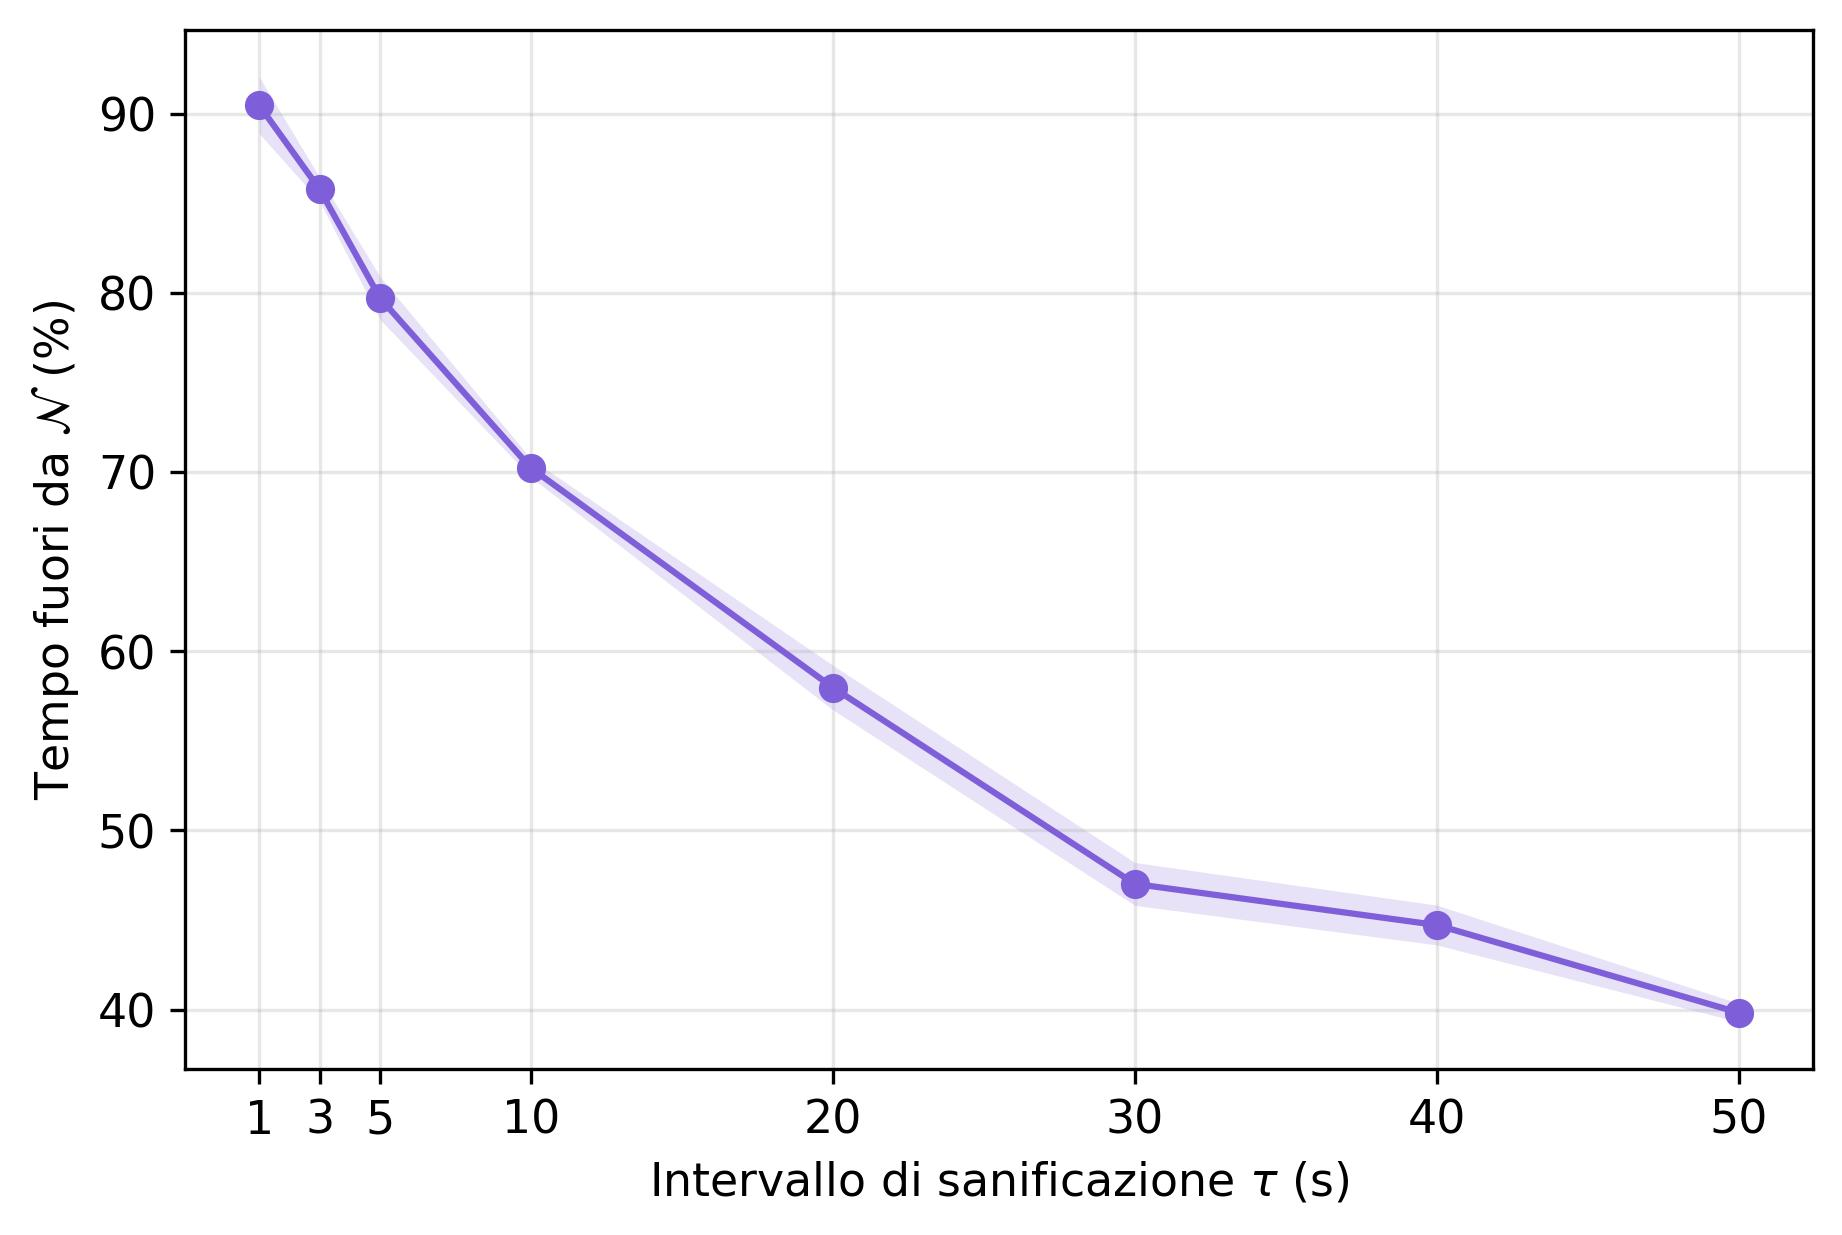
\includegraphics[width=\textwidth]{immagini/val_sanificazione/sanitize_disponibilita.jpg}
        \caption{Indisponibilità media dei nodi.}
        \label{fig:sanificazione-disponibilita}
    \end{subfigure}
    \caption{Cause del blocco dei task e indisponibilità dei nodi al variare dell'intervallo $\tau$.}
    \label{fig:sanificazione-cause-disponibilita}
\end{figure}

La ragione dei due bracci emerge dalla Figura~\ref{fig:sanificazione-cause-disponibilita}, che spiega il fenomeno dai due lati, quello dei task e quello dei nodi. A sinistra, la ripartizione per causa di blocco mostra che agli intervalli più brevi è elevata la quota di task respinti perché il nodo è in sanificazione, segnata come \emph{taint}. Con un intervallo di pochi secondi i nodi vengono messi in sanificazione di continuo, e un task ha alta probabilità di trovarli indisponibili non perché contaminati, ma perché in pulizia. Al crescere di $\tau$ questa componente si riduce fino a quasi annullarsi intorno a $\tau = 20$, dove il blocco è dovuto quasi solo alle tracce contestuali non ancora rimosse, per poi risalire agli intervalli più lunghi. 

Lo stesso fenomeno, visto dal lato dei nodi, è riassunto dall'indisponibilità media, che misura la frazione di tempo in cui un nodo si trova fuori da $\mathcal{N}$ perché in sanificazione. Essa decresce in modo monotono, da oltre il 90\% a $\tau = 1$ fino a circa il 40\% a $\tau = 50$: più spesso si sanifica, più a lungo i nodi restano indisponibili; è proprio questa indisponibilità a spiegare il braccio sinistro della U, mentre agli intervalli lunghi il braccio destro nasce dall'effetto opposto, con le tracce che permangono troppo a lungo e bloccano un numero crescente di task. I due bracci sono quindi le due facce del compromesso tra disponibilità dei nodi e reattività dello scheduling anticipato all'inizio del capitolo.

\begin{figure}[htb]
    \centering
    \begin{subfigure}[b]{0.48\textwidth}
        \centering
        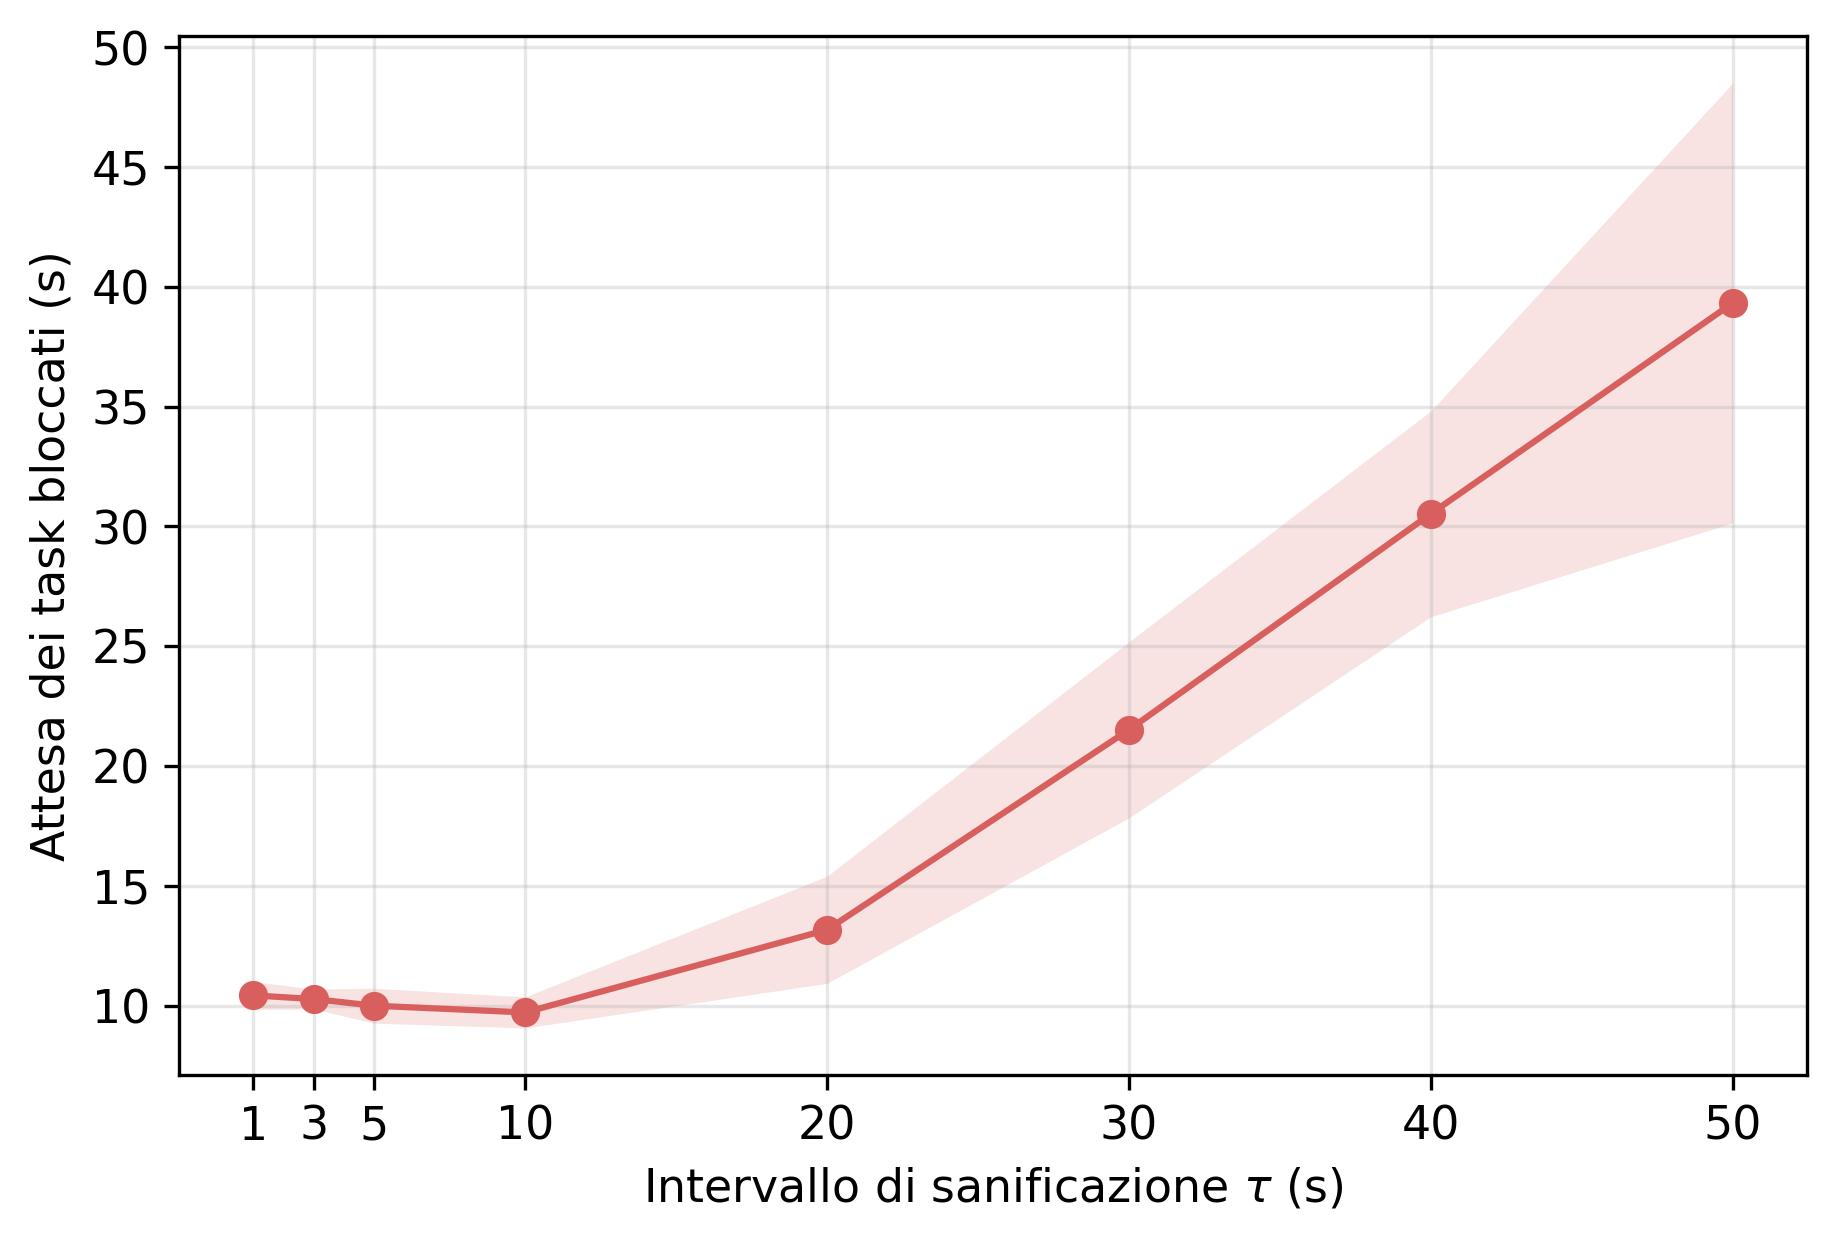
\includegraphics[width=\textwidth]{immagini/val_sanificazione/sanitize_attesa.jpg}
        \caption{Attesa media dei task bloccati.}
        \label{fig:sanificazione-attesa}
    \end{subfigure}
    \hfill
    \begin{subfigure}[b]{0.48\textwidth}
        \centering
        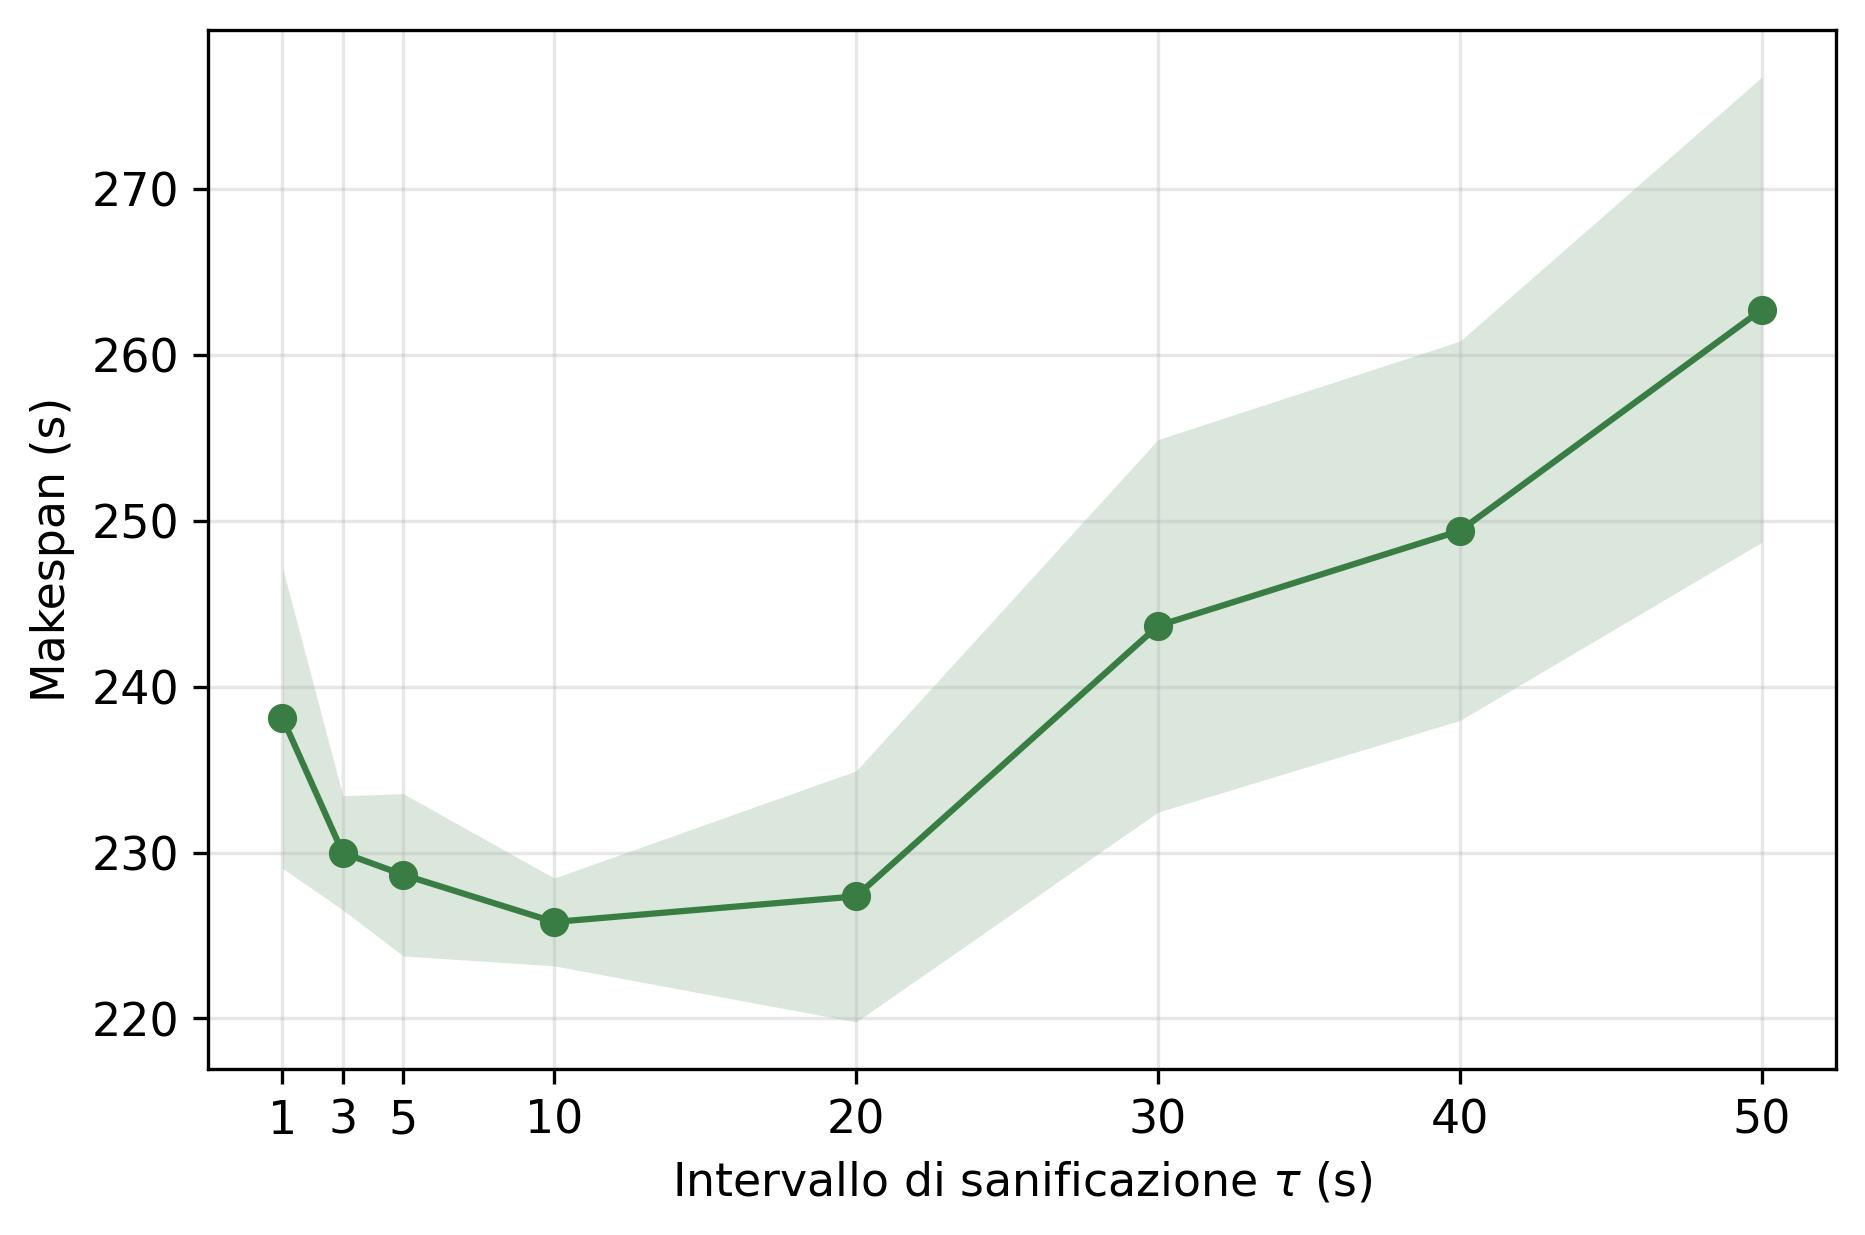
\includegraphics[width=\textwidth]{immagini/val_sanificazione/sanitize_makespan.jpg}
        \caption{Makespan del batch.}
        \label{fig:sanificazione-makespan}
    \end{subfigure}
    \caption{Costo globale della sanificazione al variare dell'intervallo $\tau$.}
    \label{fig:sanificazione-attesa-makespan}
\end{figure}

Il costo globale in termini di tempo è mostrato dalla Figura~\ref{fig:sanificazione-attesa-makespan}. L'attesa media dei task bloccati resta sui 10 secondi fino al minimo della U, per poi crescere rapidamente fino a quasi 40 secondi a $\tau = 50$. Questo chiarisce la natura asimmetrica dei due bracci: a sinistra i task vengono bloccati spesso, ma per poco tempo ciascuno, perché un nodo tornerà presto disponibile; a destra vengono bloccati meno spesso, ma chi resta bloccato attende molto più a lungo, dato che lo sblocco dipende da un ciclo di sanificazione sempre più raro. Il makespan segue anch'esso un andamento a U, molto più contenuto, con un minimo intorno ai 226 secondi nella regione ottimale e una risalita fino a circa 238 secondi a $\tau = 1$ e 263 secondi a $\tau = 50$. Anche qui la vista per batch attenua l'effetto rispetto a quella per singolo task, per via dei 200 secondi di sottomissione e della sovrapposizione delle attese, ma conferma che la regione tra 10 e 20 secondi minimizza il costo sia per il singolo task sia per il carico complessivo.

Per concludere, l'esperimento conferma l'andamento a U atteso e individua una regione ottimale dell'intervallo di sanificazione tra 10 e 20 secondi per questo carico, in cui si bilanciano i due effetti opposti. Al di sotto di questa regione la sanificazione tiene i nodi troppo spesso indisponibili, al di sopra lascia le tracce troppo a lungo sui nodi, e in entrambi i casi la latenza di scheduling peggiora.

% ------------------------------------------------------------ %

\section{Discussione e Limitazioni}
\label{sec:discussione_limitazioni}

I due esperimenti, visti insieme, misurano lo stesso compromesso di fondo anticipato all'inizio del capitolo, quello tra la disponibilità dei nodi e la reattività dello scheduling, sul quale la densità di conflitto e l'intervallo di sanificazione agiscono su lati distinti. Il primo esperimento mostra che il peso di questo compromesso cresce con il grado di conflitto, poiché più i contesti sono in conflitto tra loro più task restano bloccati in attesa che la sanificazione liberi un nodo, mentre il secondo mostra come l'intervallo di sanificazione governi il modo in cui tale attesa viene pagata, con una regione ottimale di $\tau$ in cui i nodi non sono sanificati così spesso da risultare quasi sempre indisponibili, né così di rado da restare a lungo contaminati. I due risultati si completano, dato che la densità stabilisce quanto il sistema sia esposto al blocco e la sanificazione quanto rapidamente possa liberarsene, e insieme indicano che il costo di $c_{wall}$ non è una proprietà fissa del modello ma dipende tanto dal carico sottomesso quanto dalla cadenza con cui i nodi vengono ripuliti.

Da questa lettura emerge un limite non del modello ma della strategia di sanificazione adottata, e i dati raccolti ne motivano un miglioramento in più direzioni. La sanificazione periodica, l'unica implementata nel prototipo tra quelle discusse nella Sezione~\ref{subsec:chinese_wall}, agisce a cadenza fissa e indipendentemente dallo stato dei nodi, perciò la regione ottimale individuata non è un valore universale ma dipende dal carico, collocandosi in questo caso intorno alla durata dei task, e un intervallo calibrato per un carico risulterebbe inadeguato per un altro. Una prima direzione di miglioramento sono proprio le strategie alternative già discusse nel modello, dove si osservava anche come più strategie possano essere combinate tra loro. Al posto della sola sanificazione periodica si potrebbe ad esempio adottare una combinazione di quella opportunistica e di quella basata su \emph{threshold}: la prima, intervenendo su un nodo appena questo è libero dai task attivi, mitigherebbe il braccio sinistro della curva osservata, mentre la seconda, avviando la pulizia quando la cardinalità di $\Lambda(n)$ supera una certa soglia, eviterebbe che un nodo accumuli troppi contesti e si avvicini alla saturazione.

Una seconda direzione, più sostanziale, riguarda il modo stesso in cui la sanificazione tratta il nodo e i task in esecuzione su di esso. Come descritto nella Sezione~\ref{subsec:chinese_wall}, la procedura attuale porta il nodo fuori da $\mathcal{N}$ e attende il completamento di tutti i task attivi prima di ripulirne le tracce, per cui un singolo task di lunga durata tiene il nodo indisponibile per tutti gli altri task per l'intero tempo della sua esecuzione. Si potrebbe invece rendere la pulizia parziale, lasciando il nodo in $\mathcal{N}$ e intervenendo in modo diverso sui task in base a quanto manca al loro completamento. All'avvio della sanificazione si attenderebbero soltanto i task la cui durata residua, stimata, resta sotto una certa soglia, ripulendo la loro traccia contestuale insieme a quella dei task già terminati in precedenza. I task che invece supererebbero quella soglia non verrebbero attesi, e la loro traccia resterebbe sul nodo, continuando a bloccare i soli task in conflitto con essi. In questo modo il nodo si libera di tutta la contaminazione eliminabile in tempi brevi, senza dover restare indisponibile in attesa dei pochi task più lunghi. Questo approccio però richiede di poter stimare la durata di un task, informazione che il modello attuale non possiede trattando i task come \emph{black-box}. Disporre di una stima, ricavata ad esempio dalla semantica del task, è proprio ciò che permetterebbe di decidere caso per caso se attendere il completamento di un task e ripulirne la traccia, oppure, quando la sua durata supera la soglia, procedere senza attenderlo lasciandone la traccia sul nodo. Lasciando sul nodo task ancora attivi, questa variante andrebbe accompagnata dall'estensione indicata nella Sezione~\ref{subsec:chinese_wall}, che tiene conto anche delle autorizzazioni dei rispettivi issuer.

Per finire, gli esperimenti hanno confermato le aspettative formulate senza produrre comportamenti inattesi, il che costituisce anche una verifica indiretta della correttezza del prototipo rispetto al modello teorico, ma restano alcune limitazioni, in parte già anticipate, che delimitano la portata dei risultati. La prima, discussa nella Sezione~\ref{subsec:perimetro_valutazione}, riguarda le risorse computazionali dei nodi, dato che i task, non occupando significativamente CPU o memoria, non saturano mai i nodi, mentre in un carico reale la loro saturazione costituirebbe un ulteriore fattore di ritardo, estraneo però alle politiche del modello. Una seconda deriva dall'ambiente a singola macchina descritto nella Sezione~\ref{sec:configurazione_sperimentale}, in cui tutte le componenti del cluster condividono le stesse risorse e sotto carico possono quindi introdurre leggeri ritardi non imputabili al sistema in valutazione, per cui i valori assoluti di latenza non vanno intesi come rappresentativi di un cluster di produzione reale. Infine, agli intervalli di sanificazione più lunghi una run copre pochi cicli di pulizia e la stima della latenza è dominata dalla varianza, come testimoniano le bande più ampie nella Figura~\ref{fig:sanificazione-latenza-cdf}, per cui i valori oltre l'ottimo vanno letti come tendenza più che come misure precise.
\chapter{Conclusioni}
\label{cap:conclusioni}

Questa tesi è partita da un problema concreto, quello di eseguire computazioni sui nodi di un cluster utilizzando dataset soggetti a vincoli di protezione, senza lasciare a chi sottomette le richieste la scelta di dove eseguirle, dato che gli enti esterni non hanno visibilità sull'infrastruttura e sono proprio i soggetti da cui i dati vanno protetti. Per affrontarlo si è lavorato su due fronti: sul primo è stato definito un modello che governa l'assegnazione dei task attraverso un insieme di politiche, statiche e dinamiche, dove alle condizioni di ammissibilità basate sulle proprietà dei nodi e sulla posizione dei dati, e ai criteri di costo, si affianca una politica di isolamento ispirata al modello \emph{Chinese Wall}, che tiene conto della storia delle elaborazioni su ciascun nodo; sul secondo questo modello è stato implementato in ambiente Kubernetes, sfruttando i meccanismi di estensione nativi per portare la valutazione delle politiche dalla fase di ammissione delle richieste fino alla scelta effettiva del nodo.

Una volta realizzato, il sistema è stato valutato sperimentalmente rispetto alla sua componente dinamica, l'unica il cui comportamento evolve con lo stato del cluster. Ne è emerso che il costo di questa politica non è fisso, ma nasce da un compromesso tra la disponibilità dei nodi e la reattività dello scheduling, e può quindi essere contenuto calibrando opportunamente la configurazione. Nel complesso il sistema realizza quanto si proponeva, con politiche definite centralmente e applicate in modo uniforme a ogni richiesta, e i limiti emersi riguardano le strategie adottate e il perimetro della valutazione più che l'impianto del modello.

Restano poi diversi sviluppi futuri lungo cui il lavoro potrebbe proseguire. Il più immediato nasce dalla valutazione stessa, che suggerisce di affiancare alla sanificazione periodica strategie più sofisticate, capaci di adattare la pulizia dei nodi allo stato del cluster e alla durata dei task in esecuzione anziché agire a cadenza fissa. Altre direzioni invece derivano dalle assunzioni adottate nel prototipo, che una versione più completa del sistema potrebbe gradualmente rimuovere: dare ai task una semantica propria, oltre a consentirne l'esecuzione reale al posto di un'immagine segnaposto, permetterebbe di stimarne la durata e abiliterebbe proprio le strategie di sanificazione appena accennate; la politica di isolamento, oggi riferita a ciò che è stato elaborato su un nodo, potrebbe tenere conto anche degli issuer che hanno task ancora attivi su di esso; la gestione dei dati, oggi puramente logica e limitata alla valutazione del costo del loro trasferimento, potrebbe estendersi al piano fisico, eseguendo concretamente lo spostamento o l'accesso remoto al momento della scelta del nodo; la possibilità di modificare i metadati durante l'esecuzione della pipeline aprirebbe la gestione delle modifiche concorrenti e delle decisioni che ne risultano invalidate. Infine, l'estensione a scenari multi-cluster porterebbe il sistema oltre il singolo cluster, con i problemi di coordinazione e di sincronizzazione dello stato che ne derivano. In tutti i casi si tratta di estensioni da inserire sull'infrastruttura esistente senza ridiscuterne i fondamenti, a conferma che il modello e la sua realizzazione costituiscono una base solida su cui continuare a costruire.


%
%			BIBLIOGRAFIA
%

% Si può specificare a che livello della TOC deve essere la bibliografia.
% Il default è 'chapter', per 'part' usare
% \beforebibliography[part]
\beforebibliography
\bibliographystyle{plain}
\bibliography{bibliografia}

% Pagina di chiusura
\closingpage

\end{document}